% ============================================================================
% Chapter 6: Evaluation
% Thesis: Pattern-Informed Fuzzy Deep Learning for Interpretable
%         Genotype–Phenotype Inference in Lung Adenocarcinoma
%         under Data Scarcity
% Author: Servio F. Lima
% University of Fribourg
% ============================================================================

\chapter{Evaluation of Artifacts}
\label{ch:evaluation}

This chapter presents the quantitative and qualitative evaluation of the three computational artifacts developed in this thesis.
Following the Design Science Research methodology, each artefact is evaluated against its baselines using the protocol specified in Section~\ref{sec:meth:evaluation_protocol}, and the results are interpreted in terms of the research questions defined in Section~\ref{sec:uc:clinical_questions}.

The evaluation is organised as follows.
Section~\ref{sec:eval:pattern} evaluates Artifact~1
(FuzzyArcLoss~V2 for pattern classification).
Section~\ref{sec:eval:mutation} evaluates Artifacts~2 and~3
(PI-ABMIL and FC-MIL for mutation prediction).
Section~\ref{sec:eval:literature} compares the results against the
published literature.
Section~\ref{sec:eval:interpretability} presents the qualitative
interpretability analysis.
Section~\ref{sec:eval:limitations} consolidates the data, cohort,
and evaluation-design limitations that bound the strength of the
results that follow.
Section~\ref{sec:eval:rq} synthesises the findings by answering each
research question and assessing the central hypothesis.


% ============================================================================
\section{Evaluation of Artifact 1: Pattern Classification}
\label{sec:eval:pattern}
% ============================================================================
% ============================================================================
% Section 6.1.1 — Single-Run Screening of 18 Loss Functions
% ============================================================================

\subsection{Single-Run Results: Screening of 18 Loss Functions}
\label{sec:eval:pattern:singlerun}

Prior to the rigorous K-fold evaluation, all 18 loss function variants
(Table~\ref{tab:loss_variants}) were screened on a single 80/20
train/test split (509 training tiles, 128 test tiles) to identify the
top performers for the computationally expensive multi-seed
cross-validation.
A prerequisite for meaningful loss function comparison was establishing
a correct experimental baseline.
The pipeline corrections documented in
Section~\ref{sec:uc:pipeline_fixes}---4-channel mask input, fp32
precision, and margin-free evaluation logits---raised all 18 variants
uniformly by approximately 18~percentage points in macro-F1 (from
71--76\% to 89--95\%).
Because this improvement was \emph{universal} across all loss functions,
it represents the establishment of a fair experimental foundation
rather than a contribution of any specific method.
With this corrected baseline in place, any remaining performance
differences between loss functions are attributable to the loss
functions themselves.

Table~\ref{tab:singlerun_all18} reports the single-run macro-F1 for all
18 loss functions within the corrected pipeline.
These results are based on a single data split of 128 test tiles and
are therefore subject to high variance; they serve as a screening step
to select the top~5 methods for the definitive K-fold evaluation
(Section~\ref{sec:eval:pattern:kfold}).

\begin{table}[ht!]
\centering
\small
\caption{All 18 loss functions ranked by macro-F1 on a single 80/20
split (128 test tiles).
These results motivated the selection of the top~5 methods
(marked with $\bigstar$) for the 15-run K-fold evaluation.
Results are from a single run and should \emph{not} be used as
the primary evaluation.}
\label{tab:singlerun_all18}
\begin{tabular}{c l c c l}
\hline
\textbf{Rank} & \textbf{Loss function} & \textbf{F1 (\%)} &
\textbf{Acc (\%)} & \textbf{Selected} \\
\hline
1  & SphereFace                          & 95.03 & 95.3 & $\bigstar$ \\
2  & FuzzyArcLoss V2 (Optuna)            & 94.48 & 94.5 & $\bigstar$ \\
3  & AdaptiveFace                        & 93.97 & 93.8 & \\
4  & FuzzyArcLoss V2 ClassParams         & 93.92 & 93.8 & \\
5  & FuzzyArcLoss V3 SubCenters (Optuna) & 93.73 & 93.8 & $\bigstar$ \\
6  & ArcFace                             & 93.38 & 93.8 & $\bigstar$ \\
7  & FuzzyCosFace V2                     & 93.21 & 93.0 & \\
8  & Softmax (CE)                        & 92.87 & 93.0 & $\bigstar$ \\
9  & Label Smoothing CE                  & 92.64 & 93.0 & \\
10 & FuzzyArcLoss V1                     & 92.48 & 92.2 & \\
11 & Combined Margin (Arc+Cos)           & 92.31 & 92.2 & \\
12 & FuzzyArcLoss V2 (default)           & 92.10 & 92.2 & \\
13 & FuzzySphereFace V2                  & 91.85 & 91.4 & \\
14 & CosFace                             & 91.72 & 91.4 & \\
15 & FuzzyArcLoss V3 (Optuna)            & 91.30 & 92.2 & \\
16 & Center Loss + Softmax               & 90.88 & 91.4 & \\
17 & Focal Loss                          & 90.54 & 91.4 & \\
18 & Triplet + Angular                   & 89.23 & 89.8 & \\
\hline
\end{tabular}
\end{table}

\begin{figure}[ht!]
\centering
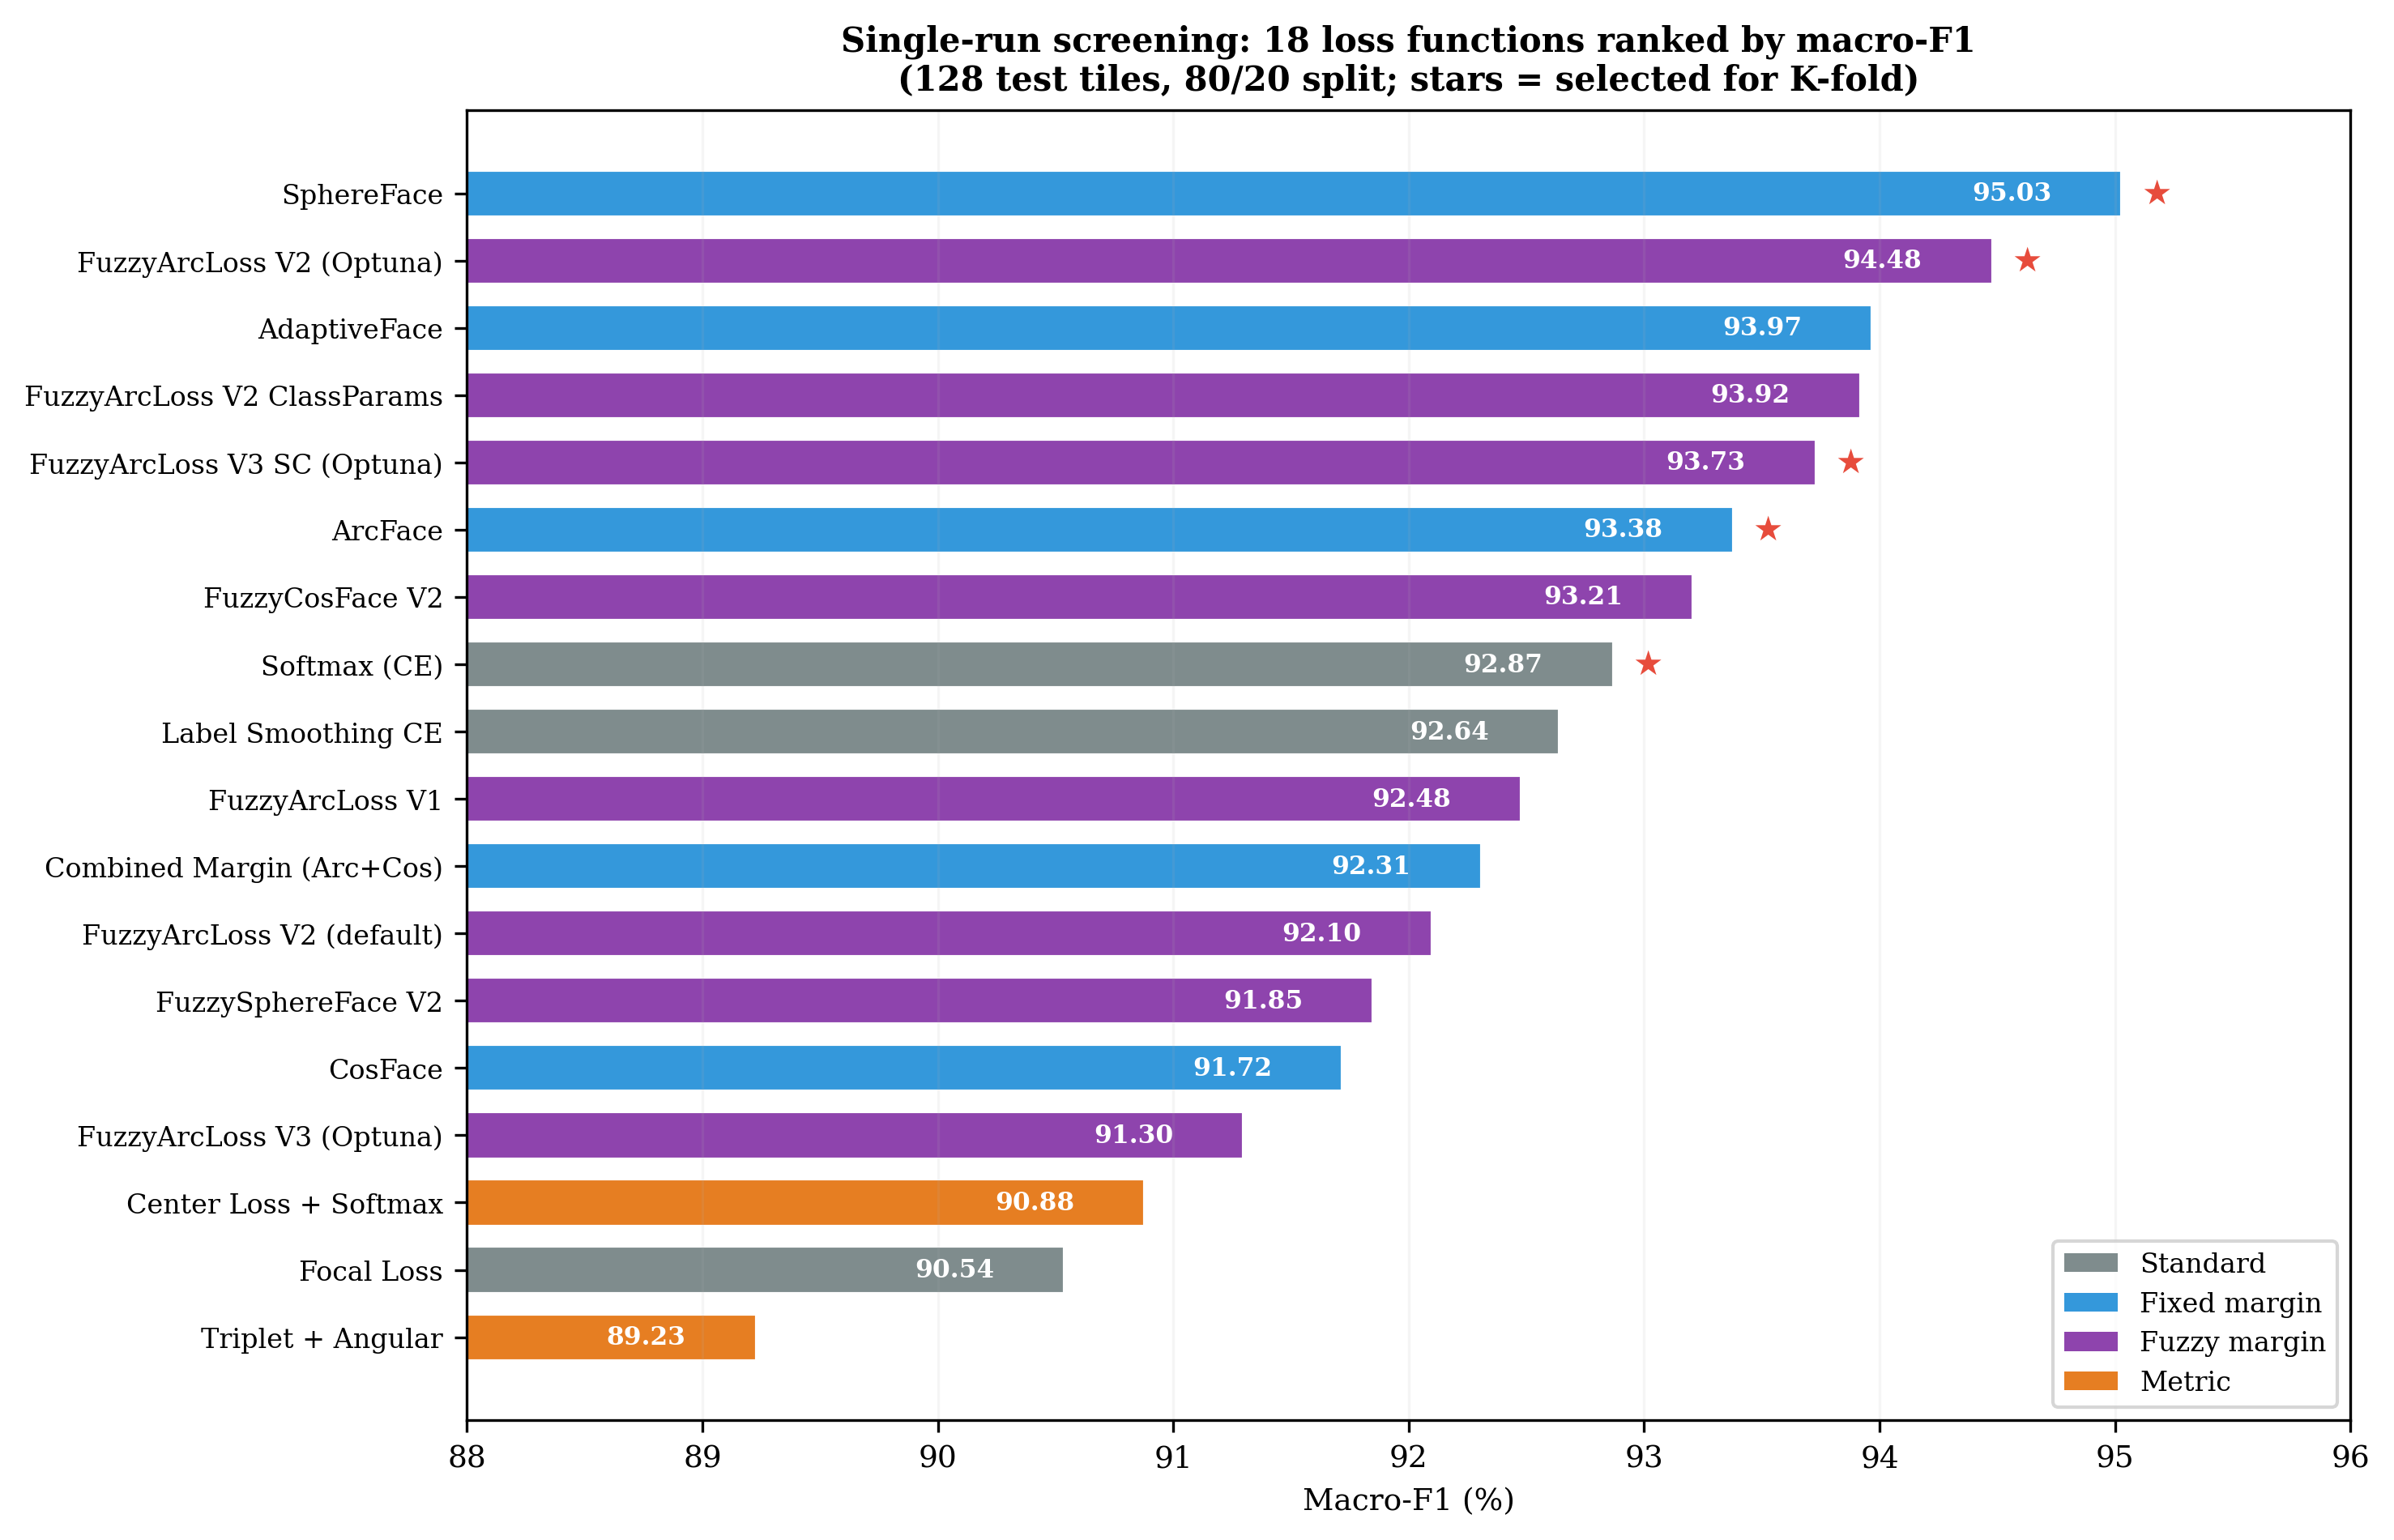
\includegraphics[width=0.92\textwidth]{chapters/figures/singlerun_18losses_bar.png}
\caption[Single-run screening: 18 loss functions]{%
    Bar chart of Table~\ref{tab:singlerun_all18}.
    All 18 loss functions ranked by macro-F1 on a single 80/20 split.
    Colour indicates loss family (grey = standard, blue = fixed margin,
    purple = fuzzy margin, orange = metric learning).
    Stars mark the five methods selected for the 15-run K-fold
    evaluation.
    SphereFace ranks first in this single run but drops to last
    in the K-fold evaluation (Table~\ref{tab:kfold_f1}).}
\label{fig:singlerun_bar}
\end{figure}

Two observations from the single-run screening motivated the K-fold
evaluation design.
First, SphereFace ranked first (95.03\%) and FuzzyArcLoss~V2 second
(94.48\%), separated by only 0.55~pp on 128 test samples---well within
the expected run-to-run variance of $\pm 0.8$~pp.
The question of which method truly generalises better could not be
resolved without multi-run evaluation.
Second, the top~5 methods spanned three categories: fixed-margin
(SphereFace, ArcFace), fuzzy-adaptive (FuzzyArcLoss~V2, V3~SubCenters),
and non-angular (Softmax~CE), ensuring a comprehensive comparison across
paradigms.

\textbf{Selection criterion for K-fold.}
The top~5 methods were selected based on two principles:
(a)~coverage of all three loss paradigms (fixed angular margin,
fuzzy-adaptive angular margin, and standard cross-entropy), and
(b)~the top single-run performer from each paradigm.
AdaptiveFace and FuzzyArcLoss~V2~ClassParams were excluded despite
strong single-run results because they are conceptual variants of the
methods already selected (ArcFace and V2~Optuna, respectively), and the
computational cost of 15 runs per method ($\sim$2.2~hours each)
constrained the number of methods.


% ============================================================================
% Section 6.1.2 — K-Fold Evaluation: Primary Results (RQ1)
% ============================================================================

\subsection{K-Fold Evaluation: Primary Results (RQ1)}
\label{sec:eval:pattern:kfold}

The primary evaluation employed 5-fold stratified cross-validation
repeated with 3 random seeds (42, 123, 2026), yielding 15 independent
runs per method (75 total training runs across 5 methods).
Table~\ref{tab:kfold_f1} reports the final rankings.

\begin{table}[ht!]
\centering
\caption{Pattern classification: 15-run evaluation
(5-fold $\times$ 3 seeds) on 637 annotated tiles across six LUAD
histological classes.
Mean macro-F1 $\pm$ standard deviation with 95\% confidence intervals.}
\label{tab:kfold_f1}
\small
\setlength{\tabcolsep}{5pt}
\begin{tabular}{@{}c l c c c c@{}}
\hline
\textbf{Rank} & \textbf{Method} & \textbf{Mean F1 (\%)} &
\textbf{$\pm$ Std} & \textbf{95\% CI} & \textbf{Mean Acc (\%)} \\
\hline
1 & \textbf{FuzzyArcLoss V2 (Optuna)} & \textbf{92.31} & 2.04 &
  [91.3, 93.3] & 93.46 \\
2 & ArcFace & 92.17 & 2.15 & [91.1, 93.3] & 93.51 \\
3 & FuzzyArcLoss V3 SubCenters & 91.79 & 2.12 & [90.7, 92.9] & 93.30 \\
4 & Softmax (CE) & 91.53 & 1.87 & [90.6, 92.5] & 92.73 \\
5 & SphereFace & 90.03 & 2.51 & [88.8, 91.3] & 91.89 \\
\hline
\end{tabular}
\end{table}

\begin{figure}[ht!]
\centering
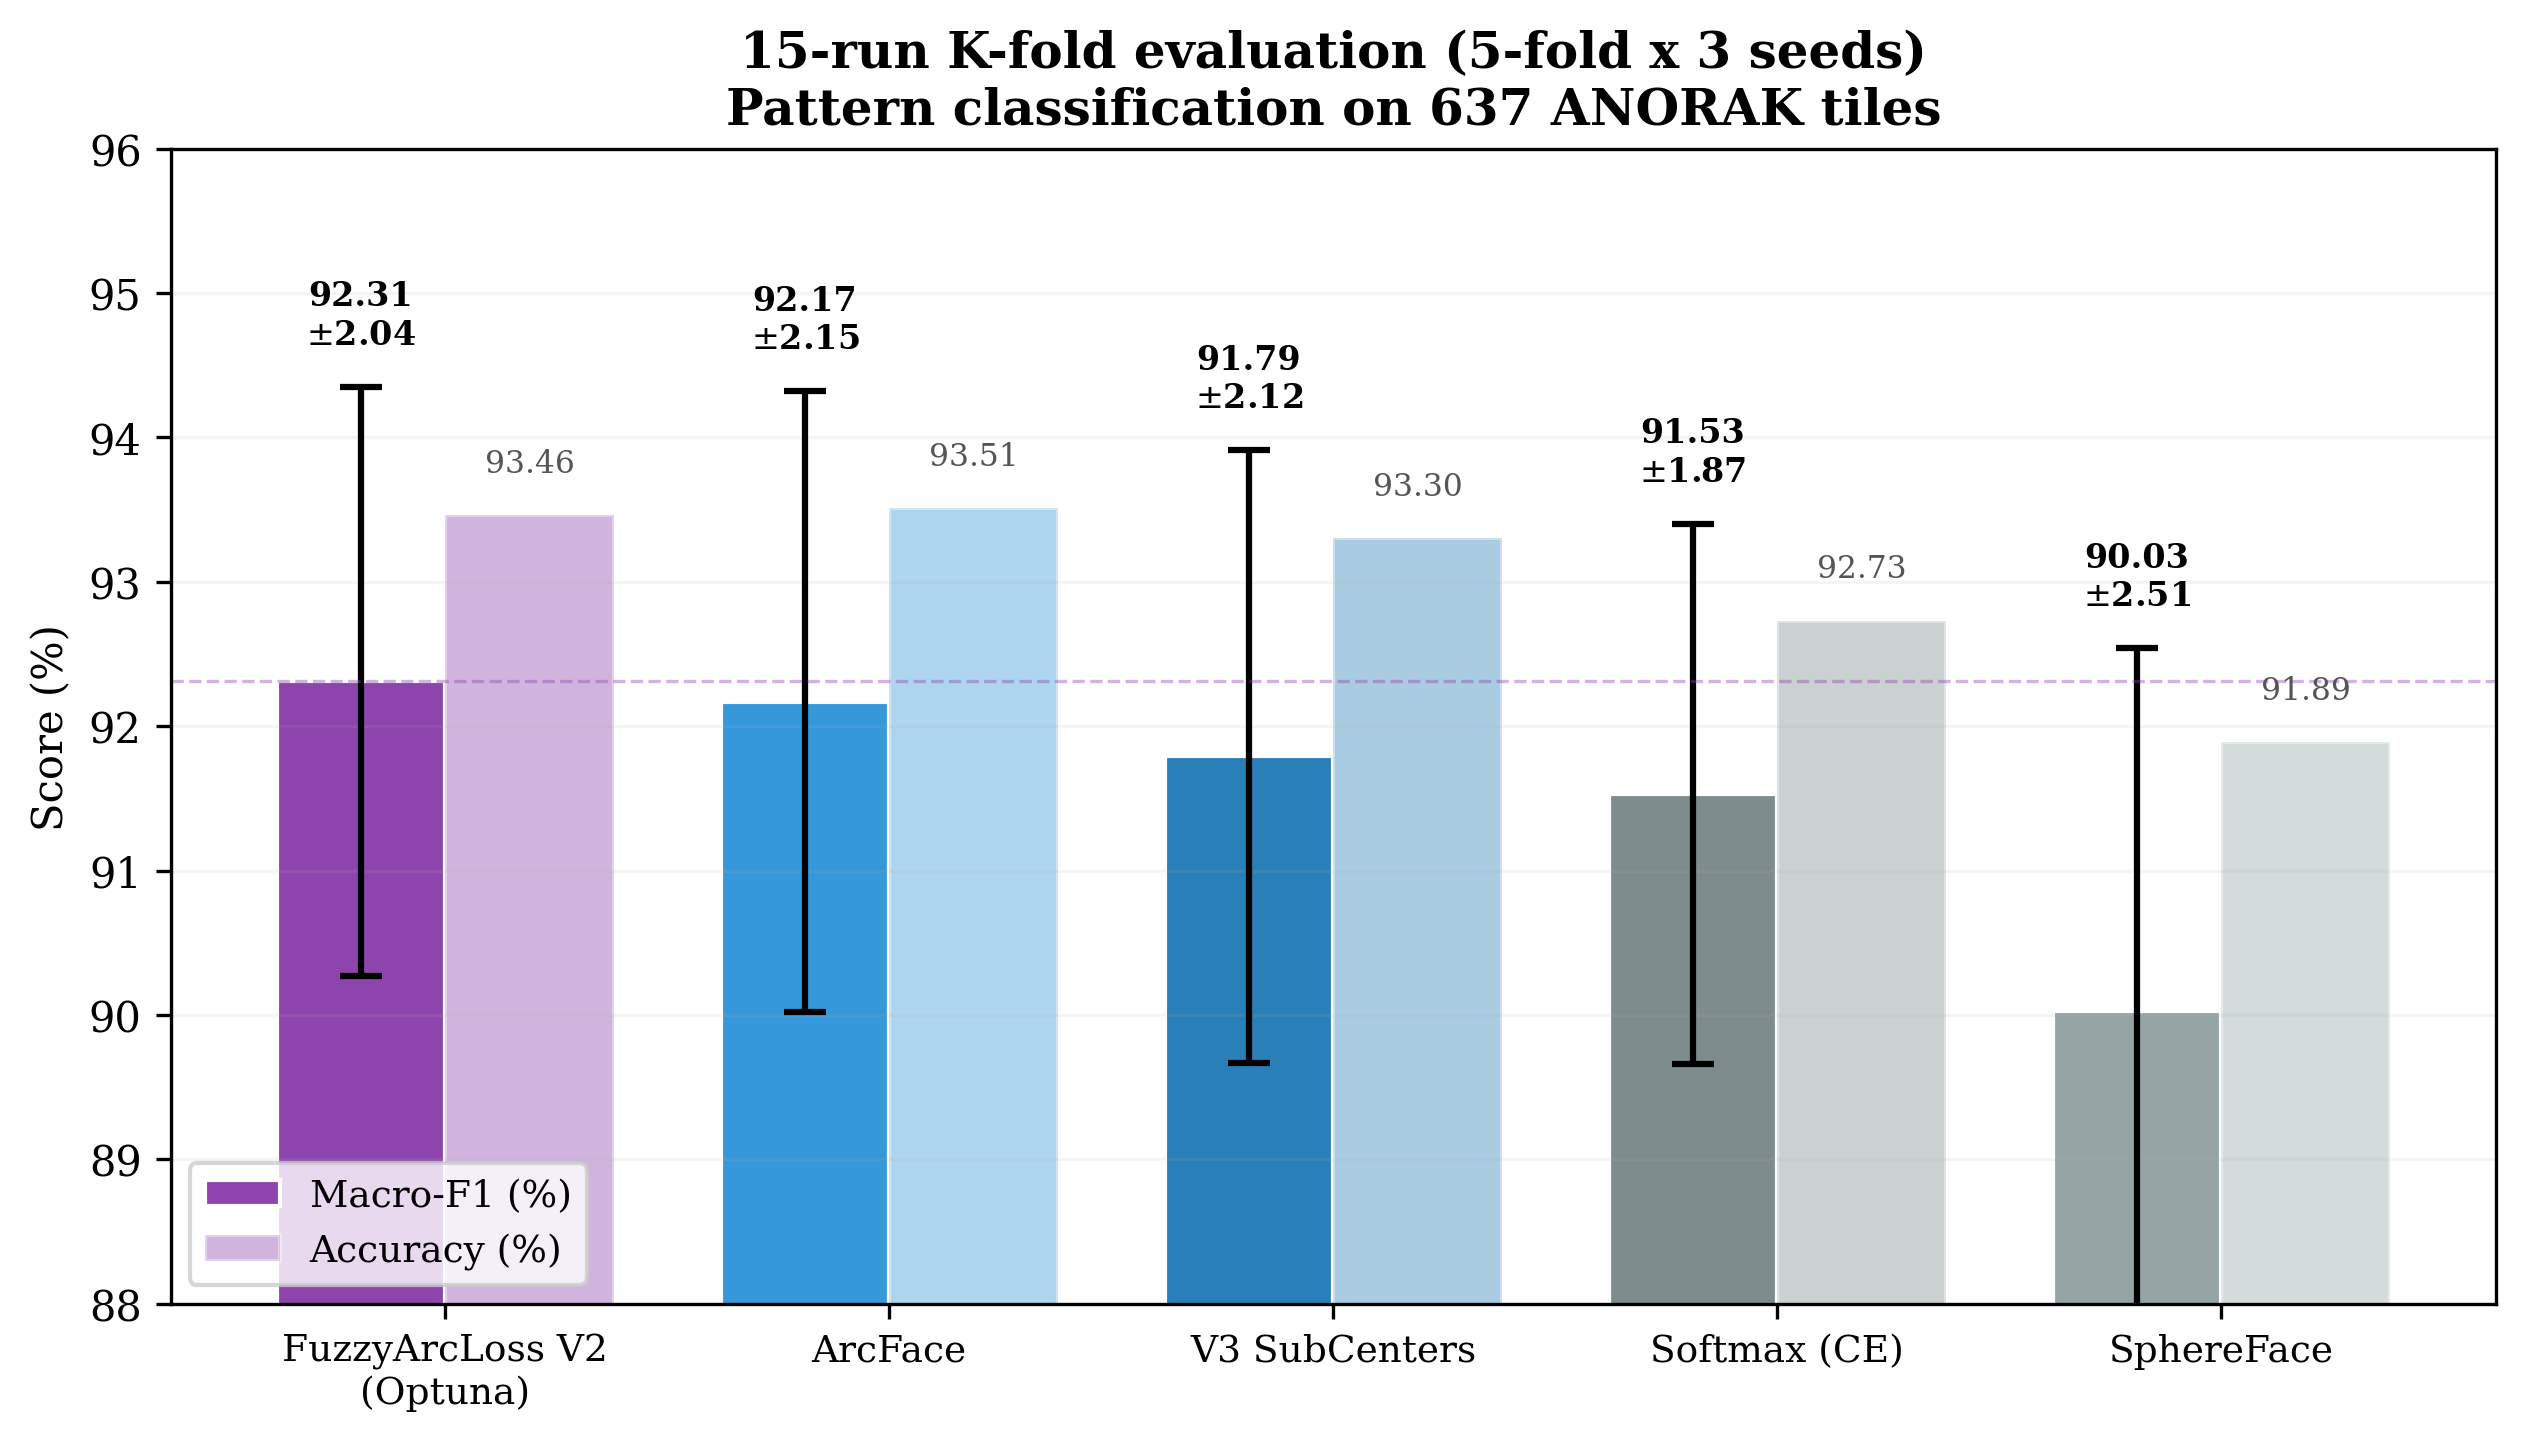
\includegraphics[width=0.85\textwidth]{chapters/figures/kfold_5methods_bar.png}
\caption[K-fold evaluation: 5 methods]{%
    Bar chart of Table~\ref{tab:kfold_f1}.
    Mean macro-F1 (solid bars with error bars $\pm$ std) and mean
    accuracy (translucent bars) across 15 independent runs.
    FuzzyArcLoss~V2 (purple) ranks first in macro-F1 (92.31\%).
    The ranking reversal from the single-run screening
    (Figure~\ref{fig:singlerun_bar}) is evident: SphereFace drops
    from 1st to 5th.}
\label{fig:kfold_bar}
\end{figure}

\textbf{Key finding: ranking reversal.}
FuzzyArcLoss~V2 achieves the highest mean macro-F1 of $92.31\% \pm 2.04$
across 15 runs, while SphereFace---which appeared to be the top performer
in the single-run screening (Table~\ref{tab:singlerun_all18})---drops to
last place with $90.03\% \pm 2.51$.
SphereFace's single-run result of 95.03\% was a favourable split artefact
that the multi-run evaluation corrects by a full 5 percentage points.
This reversal underscores the necessity of multi-run evaluation on small
datasets: any conclusion drawn from a single split of 128 test samples
would have been misleading.


\subsubsection{Statistical Significance Analysis}
\label{sec:eval:pattern:stats}

Table~\ref{tab:pattern_stats} reports pairwise statistical comparisons of
FuzzyArcLoss~V2 against each competitor, using paired $t$-tests on the 15
fold-level macro-F1 values, Cohen's $d$ effect sizes, and win rates.

\begin{table}[ht!]
\centering
\caption{Statistical comparison of FuzzyArcLoss~V2 against baseline loss
functions (15 paired runs).
Significant results ($p < 0.05$) are marked with~$^{*}$.
Win rate counts the number of runs (out of~15) where V2 achieved
strictly higher macro-F1.}
\label{tab:pattern_stats}
\resizebox{\textwidth}{!}{%
\begin{tabular}{l c c c c c l}
\hline
\textbf{Comparison (V2 vs.)} & \textbf{$\Delta$ F1} &
\textbf{$p$-value} & \textbf{Cohen's $d$} & \textbf{V2 wins} &
\textbf{Interpretation} \\
\hline
SphereFace &
  $+$2.28\,pp & $0.001^{*}$ & 1.00 (large) & 14/15 &
  V2 significantly better \\
Softmax (CE) &
  $+$0.78\,pp & 0.138 & 0.39 (small) & 9/15$^{\dagger}$ &
  V2 edges Softmax; not significant \\
V3 SubCenters &
  $+$0.51\,pp & 0.148 & 0.25 (small) & 10/15 &
  V2 edges V3; not significant \\
ArcFace &
  $+$0.14\,pp & 0.651 & 0.07 (negligible) & 9/15 &
  Essentially tied \\
\hline
\end{tabular}}%
\begin{flushleft}
\footnotesize
$^{\dagger}$Plus 1 exact tie (run at seed=2026, fold=4:
both methods achieved 92.2\% macro-F1).
\end{flushleft}
\end{table}

The comparison between V2 and SphereFace is statistically significant
($p = 0.001$) with a large effect size (Cohen's $d = 1.00$) and V2
winning 14 of 15 runs.
SphereFace's large fixed multiplicative margin ($m = 4$) produces the
highest variance among all methods (std = 2.51), suggesting that its
aggressive margin destabilises training on certain data splits.
The single run where SphereFace outperformed V2 (seed=123, fold=3:
SphereFace 92.4\% vs V2 91.7\%) was the only fold where SphereFace's
aggressive margin happened to benefit rather than harm generalisation.
FuzzyArcLoss~V2's adaptive membership, which reduces the penalty for
ambiguous samples near class boundaries, produces more consistent
performance across splits.

The differences between V2 and ArcFace ($+$0.14~pp, $p = 0.651$),
V3~SubCenters ($+$0.51~pp, $p = 0.148$), and Softmax~CE ($+$0.78~pp,
$p = 0.138$; all values from Table~\ref{tab:pattern_stats}) are not
statistically significant at $p < 0.05$.
However, the consistent ranking---V2 first in all comparisons---and the
directional advantage across 9--10 of 15 runs suggest a real but small
effect that the 15-run protocol lacks power to confirm.
With $n = 15$ paired observations, the minimum detectable effect at
80\% power and $\alpha = 0.05$ is approximately $d \approx 0.78$,
meaning that only large effects (such as the V2-vs-SphereFace gap) can
be reliably detected.


\subsubsection{Per-Class Analysis}
\label{sec:eval:pattern:perclass}

The per-class F1 scores reveal where FuzzyArcLoss~V2's adaptive margin
provides the greatest benefit and where all methods converge.

\begin{table}[ht!]
\centering
\small
\caption{Per-class F1 scores (\%, mean $\pm$ std across 15 runs) for
the five evaluated methods.
The six classes are the ANORAK-annotated LUAD histological growth
patterns: cribriform (Cri), micropapillary (MPap), solid (Sol),
papillary (Pap), acinar (Aci), and lepidic (Lep).
Cribriform, with only $\sim$55 training samples, is the hardest class.}
\label{tab:perclass_f1}

\begin{tabular}{l c c c c c c}
\hline
\textbf{Method} &
  {\textbf{Cribri.}} & {\textbf{Micropap.}} & {\textbf{Solid}} &
  {\textbf{Papillary}} & {\textbf{Acinar}} & {\textbf{Lepidic}} \\
\hline
FuzzyArcLoss V2 &
  \textbf{83.6}$\pm$9.2 & 93.8$\pm$3.6 & 94.6$\pm$3.1 &
  91.8$\pm$2.5 & \textbf{95.3}$\pm$1.9 & 94.8$\pm$3.7 \\
ArcFace &
  81.4$\pm$10.0 & \textbf{94.9}$\pm$3.4 & \textbf{95.0}$\pm$2.9 &
  \textbf{92.6}$\pm$3.8 & 95.2$\pm$2.2 & 93.9$\pm$4.4 \\
V3 SubCenters &
  79.1$\pm$10.5 & 94.4$\pm$3.6 & 94.3$\pm$2.4 &
  92.4$\pm$3.3 & 95.2$\pm$1.6 & \textbf{95.4}$\pm$3.7 \\
Softmax (CE) &
  81.5$\pm$10.4 & 94.3$\pm$6.0 & 94.7$\pm$2.3 &
  90.6$\pm$3.8 & 94.3$\pm$2.0 & 93.8$\pm$4.6 \\
SphereFace &
  76.1$\pm$12.8 & 91.2$\pm$8.2 & 94.2$\pm$2.5 &
  91.0$\pm$4.1 & 93.5$\pm$2.4 & 94.3$\pm$4.8 \\
\hline
\end{tabular}
\end{table}

\begin{figure}[ht!]
\centering
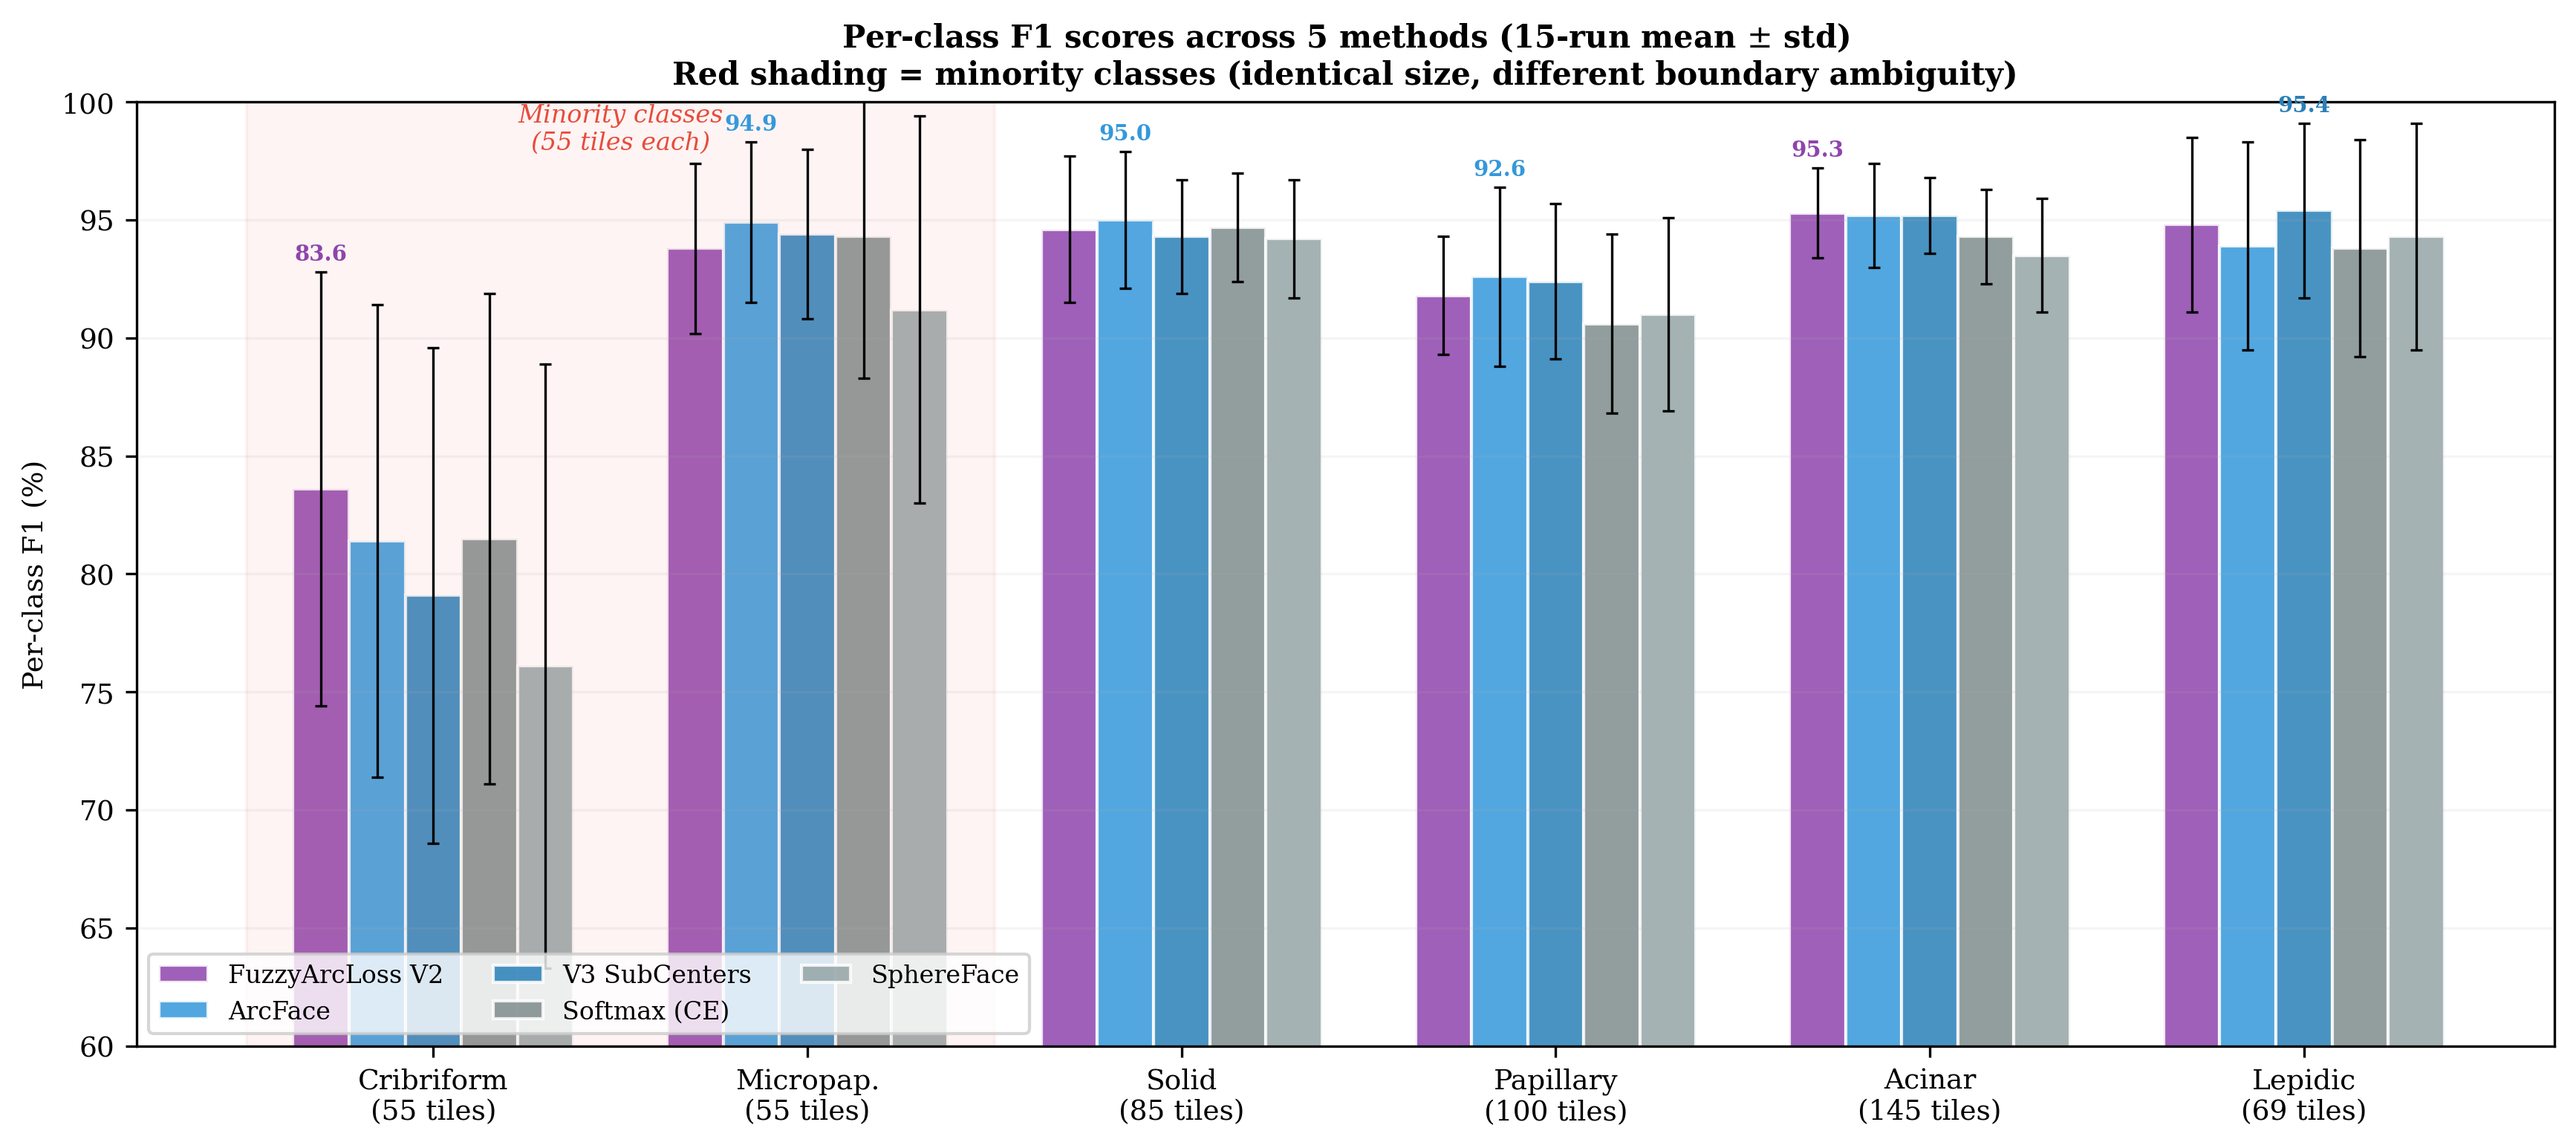
\includegraphics[width=\textwidth]{chapters/figures/perclass_f1_bar.png}
\caption[Per-class F1 across 5 methods]{%
    Bar chart of Table~\ref{tab:perclass_f1}.
    Per-class F1 (mean $\pm$ std across 15 runs) for the five
    evaluated methods.
    Red shading highlights the two minority classes (cribriform and
    micropapillary, both 55 training tiles---identical
    \emph{class size}, defined as per-class training-tile count).
    Despite identical sample counts, V2 leads on cribriform
    (ambiguous boundary with acinar) but not on micropapillary
    (visually distinctive), illustrating boundary-dependent
    rather than class-size-dependent behaviour.}
\label{fig:perclass_f1_bar}
\end{figure}

Three findings emerge from the per-class analysis.

\textbf{First, FuzzyArcLoss~V2 achieves the highest \emph{mean} F1 on
the cribriform class} (83.6\% versus ArcFace's 81.4\% and SphereFace's
76.1\%), \textbf{but not on micropapillary} (93.8\% versus ArcFace's
94.9\%), \textbf{despite both being minority classes with identical
sample counts ($\sim$55 training tiles).}
A caveat is necessary: the cribriform standard deviations are high
across all methods ($\pm 9.2$--$12.8$), reflecting the inherent
difficulty of this class on $\sim$55 tiles with 5-fold splitting.
The $+2.2$~pp mean advantage of V2 over ArcFace on cribriform
(Table~\ref{tab:perclass_f1}) is
therefore a \emph{directional trend} rather than a statistically
significant per-class difference; the large overlap in confidence
intervals ($[74.4, 92.8]$ vs $[71.4, 91.4]$) precludes a strong
per-class claim.
Nevertheless, the \emph{direction} of the effect---V2 leads on the
ambiguous-boundary class but trails on the crisp-boundary class---is
itself the informative finding: V2's advantage is
\emph{morphological-boundary-dependent, not class-size-dependent}.
Two definitions are used in the rest of the thesis when this
phrase appears.
\textbf{(i)~Boundary} refers to the \emph{decision surface
between two adjacent histological pattern classes}, parameterised
by their inter-annotator agreement
($\kappa \approx 0.38$ for cribriform--acinar
\cite{thunnissen2012reproducibility} vs.\ a much higher
agreement for micropapillary--solid): a boundary is
\emph{ambiguous} when adjacent classes overlap morphologically
and expert pathologists disagree on the cut, and
\emph{crisp} when the visual distinction is unambiguous.
\textbf{(ii)~Class size} denotes the number of training tiles
available for a given class (cribriform and micropapillary both
have $55$ training tiles, so class size is held constant in this
comparison; \emph{not} the size of the overall training dataset).
Cribriform is a high-grade acinar variant whose morphological boundary
with acinar is genuinely ambiguous---the confusion matrix
(Figure~\ref{fig:confusion_matrix}) confirms cribriform--acinar as
the primary error mode, and inter-observer agreement for this
distinction is low ($\kappa \approx 0.38$~\cite{thunnissen2012reproducibility}).
V2's reduced margin for low-confidence tiles prevents the model from
memorising arbitrary labels at this fuzzy boundary, producing the
$+2.2$~pp advantage over ArcFace and $+7.5$~pp over SphereFace
(Table~\ref{tab:perclass_f1}).
SphereFace's 76.1\% cribriform F1---combined with the highest per-class
standard deviation (12.8)---confirms that its fixed multiplicative
margin of $m = 4$ is too aggressive for ambiguous boundaries.

Micropapillary, by contrast, is visually \emph{distinctive}: floating
cell clusters lacking fibrovascular cores are morphologically
dissimilar to all other patterns.
ArcFace's fixed full margin is appropriate here because the
class boundary is relatively crisp; V2's gentle margin for uncertain
samples provides no advantage---and may slightly relax the angular
separation---on tiles that are not genuinely ambiguous
(ArcFace: 94.9\% vs V2: 93.8\%).

\textbf{The implication is that V2's fuzzy membership modulation
targets morphological ambiguity, not class rarity}: it helps where
inter-class transitions are gradual (cribriform--acinar), not where
classes are merely small (micropapillary).

\textbf{Third, the acinar and lepidic classes exceed 93\% F1 across
all methods}, indicating that these morphologically distinctive
patterns are well-separated in the embedding space regardless of the
loss function.

\textbf{Fourth, the differentiation among methods concentrates on
classes with ambiguous boundaries.}
The inter-method F1 range (best minus worst) is 7.5~pp for cribriform
(ambiguous boundary with acinar), 3.7~pp for micropapillary
(moderate boundary ambiguity with papillary), and only 0.8~pp for
solid (visually distinctive).
This confirms that the choice of loss function matters most where
morphological boundaries are gradual---precisely the regime for which
FuzzyArcLoss~V2 was designed.
The implication for practitioners is that V2's benefit should be
evaluated per-class based on boundary ambiguity, not assumed to
apply uniformly to all minority classes.

Figure~\ref{fig:boundary_vs_size} visualises this distinction.

\begin{figure}[ht!]
\centering
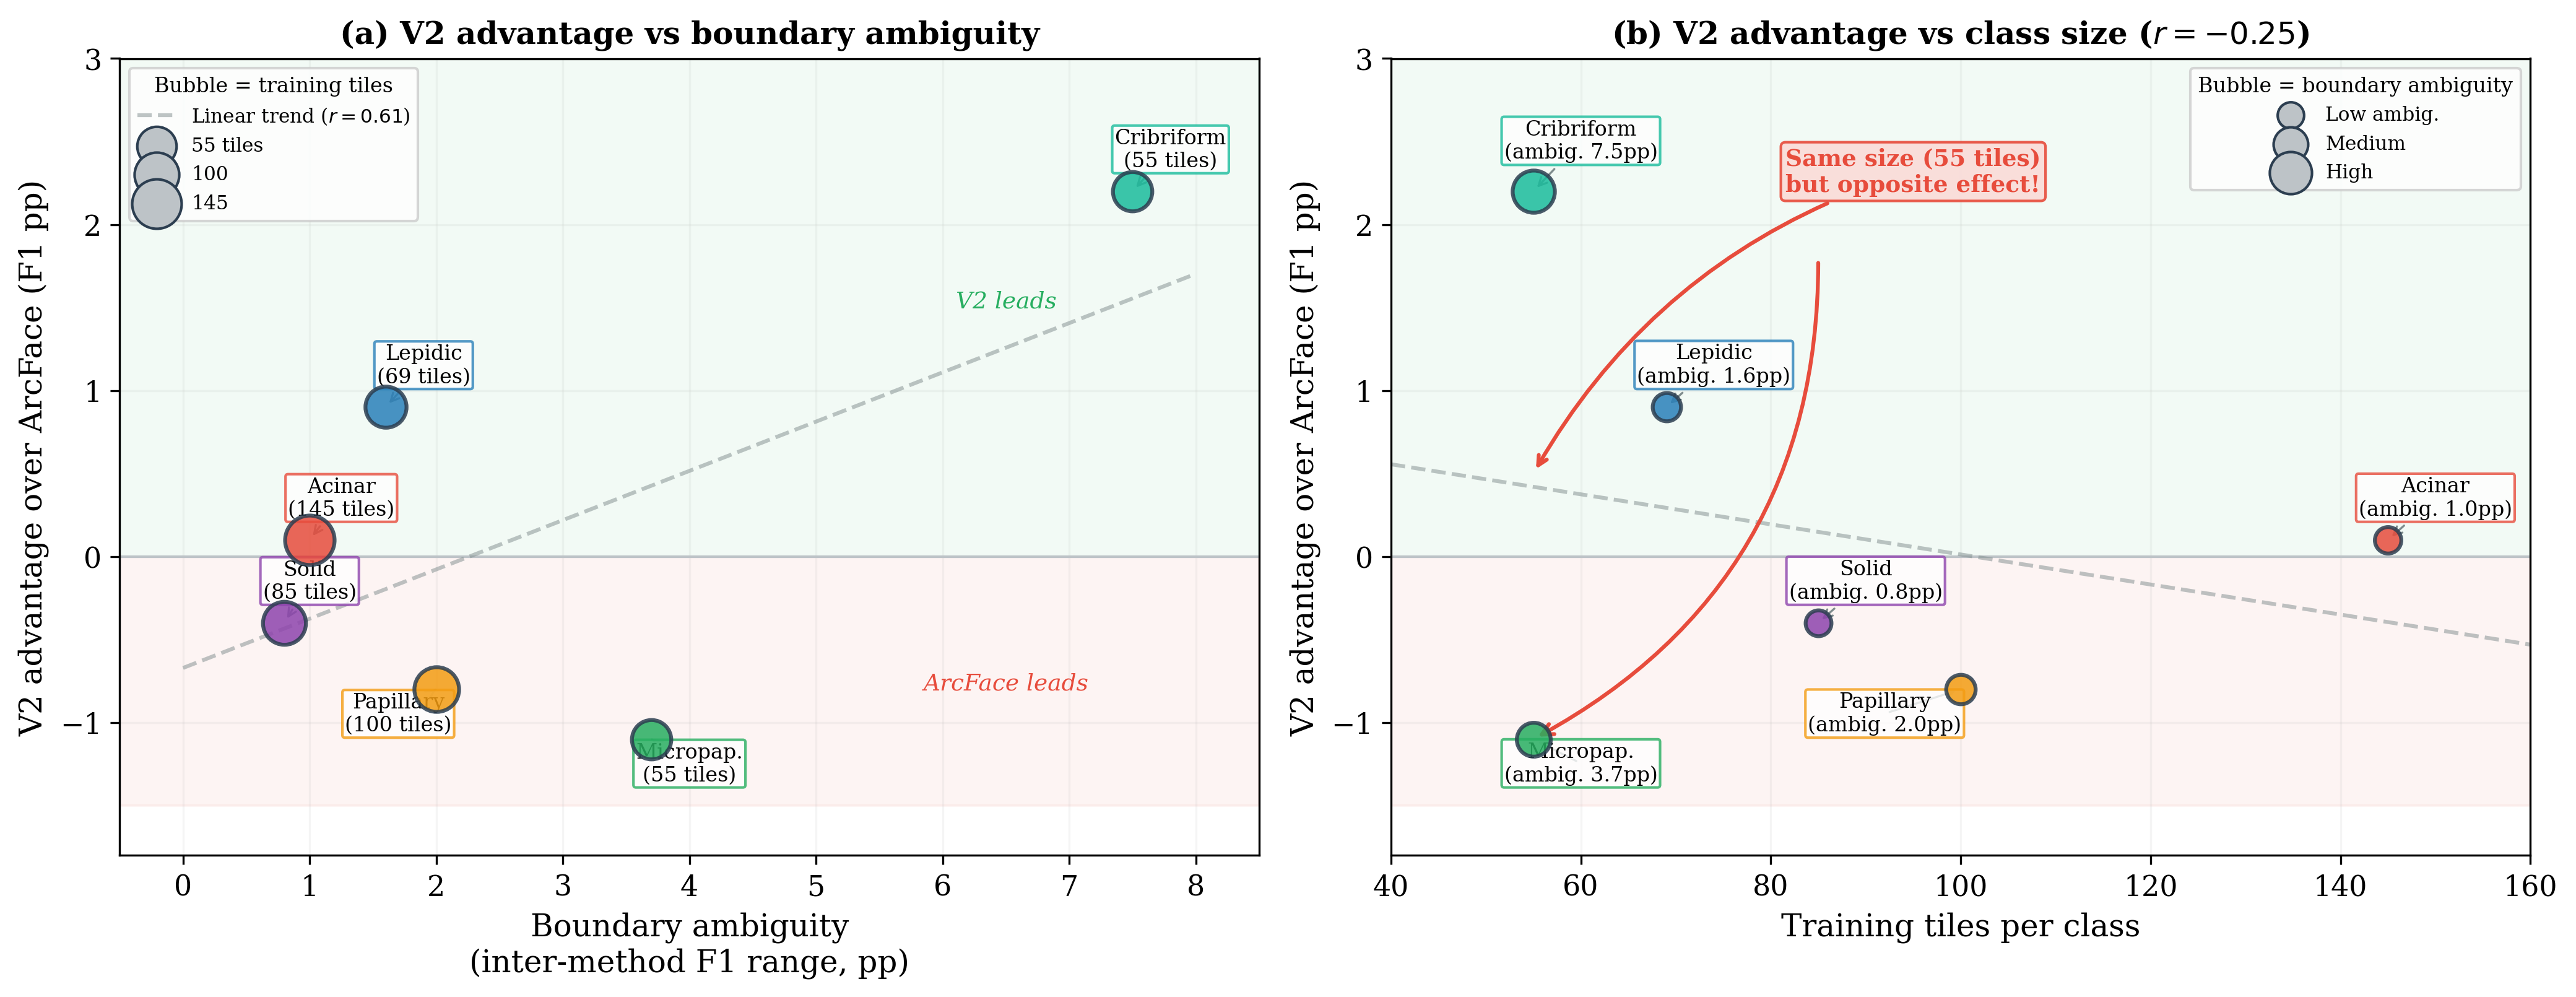
\includegraphics[width=\textwidth]{chapters/figures/boundary_vs_size_v2.png}
\caption[V2 advantage: boundary-dependent, not class-size-dependent]{%
    FuzzyArcLoss~V2's per-class F1 advantage over ArcFace
    ($\Delta$\,pp) plotted against boundary ambiguity and class
    size (\emph{class size} = number of training tiles for that
    class; \emph{not} dataset size).
    \textbf{(a)}~V2 advantage vs boundary ambiguity (inter-method F1
    range): cribriform (high ambiguity, $+2.2$~pp) and micropapillary
    (moderate ambiguity, $-1.1$~pp) have the same training size
    (55 tiles) but opposite effects.
    The positive correlation ($r = 0.61$) confirms that V2's benefit
    increases with boundary ambiguity.
    \textbf{(b)}~V2 advantage vs class size ($r = -0.25$): no
    meaningful correlation.
    Cribriform and micropapillary (both 55 tiles, circled) demonstrate
    that identical sample count produces opposite V2 deltas when
    boundary ambiguity differs.
    Bubble size encodes training tiles (a) or boundary ambiguity (b).
    Green region: V2 leads; red region: ArcFace leads.}
\label{fig:boundary_vs_size}
\end{figure}

\subsubsection{Optuna Hyperparameter Analysis}
\label{sec:eval:pattern:optuna}

The Optuna Bayesian search over 50 trials identified the optimal
configuration $s^{*} = 46.1$, $m^{*} = 0.518$, $\tau^{*} = 0.448$
for FuzzyArcLoss~V2.
The V2 Optuna model achieved avgPR = 0.9306 on the screening split,
outperforming the V3~SubCenters Optuna search
(avgPR = 0.9127) by $+1.8$ percentage points.

The convergence of the margin $m$ to a value close to the ArcFace
default ($m = 0.5$) while the scale $s$ diverged significantly
($46.1$ versus the default $30$) confirms that the performance advantage
of V2 arises from the \emph{modulation mechanism} rather than from the
raw margin magnitude.
A higher scale sharpens the softmax distribution, making the model more
decisive.
In standard ArcFace, this would risk training instability for ambiguous
samples.
In FuzzyArcLoss~V2, the fuzzy membership acts as a ``safety valve'': the
reduced margin for uncertain samples ($\mu_{i} \approx 0.3$--$0.5$)
compensates for the aggressive scale, preventing gradient explosion at
decision boundaries.
The Optuna search also confirmed that Label Smoothing~$+$~Focal weighting
is the optimal auxiliary loss for V2 (all top-4 trials agreed), consistent
with the theoretical complementarity of output-level label smoothing and
embedding-level fuzzy margin softening.


\subsubsection{Summary of Pattern Classification Evaluation}
\label{sec:eval:pattern:summary}

The 15-run K-fold evaluation resolves the ambiguity of the single-run
screening and yields the following conclusions for RQ1:

\begin{enumerate}
    \item FuzzyArcLoss~V2 ranks first with 92.31\% mean macro-F1,
    consistently ahead of all baselines across 15 independent runs.

    \item The advantage over SphereFace is statistically significant
    ($p = 0.001$, Cohen's $d = 1.00$, 14/15 wins), establishing that
    V2's fuzzy-adaptive margin produces reliably better generalisation
    than SphereFace's aggressive fixed multiplicative margin on this
    small dataset.

    \item V2 ranks first in \emph{every} pairwise comparison: $+$0.14~pp
    over ArcFace, $+$0.51~pp over V3~SubCenters, and $+$0.78~pp over
    Softmax~CE (Table~\ref{tab:pattern_stats}), winning 9--10 of 15 runs
    in each case.
    These differences do not reach $p < 0.05$ because with only
    $n = 15$ paired observations, the protocol can only detect large
    effects ($d \geq 0.78$); the consistent directional advantage
    across all comparisons is nonetheless informative.

    \item V2's per-class advantage is boundary-dependent, not
    class-size-dependent (\emph{class size} = number of training
    tiles per class; cribriform and micropapillary both have $55$):
    V2 leads on cribriform ($+$2.2~pp mean over ArcFace), whose
    boundary with acinar is genuinely ambiguous, but not on
    micropapillary ($-$1.1~pp), an equally rare class with a
    crisp visual boundary
    (Figure~\ref{fig:boundary_vs_size}).
    The high per-class standard deviations ($\pm$9--13) mean this is a
    directional trend rather than a statistically significant per-class
    difference, but the \emph{pattern}---advantage at ambiguous
    boundaries, no advantage at crisp ones---is consistent with V2's
    design principle.

    \item The systematic pipeline corrections (4-channel mask input,
    fp32 precision, margin-free evaluation logits) established a correct
    experimental baseline, raising all methods uniformly by $+$18~pp.
    This universal improvement is not attributable to any loss function
    but rather provides the fair foundation upon which the loss function
    comparisons above become meaningful.
    The lesson is that implementation details are as critical as
    algorithmic innovation when applying angular margin losses to small
    histopathological datasets.
\end{enumerate}


\subsubsection{Confusion Matrix and Expert Validation}
\label{sec:eval:pattern:confusion}

To understand class-level error patterns beyond aggregate F1 scores,
Figure~\ref{fig:confusion_matrix} presents the confusion matrix for
FuzzyArcLoss~V2 on the ANORAK validation set (138~tiles, 80/20 split,
seed~42), with class names mapped to the official Zenodo annotation
scheme (Table~\ref{tab:variant_types_patterns}).

\begin{figure}[ht!]
\centering
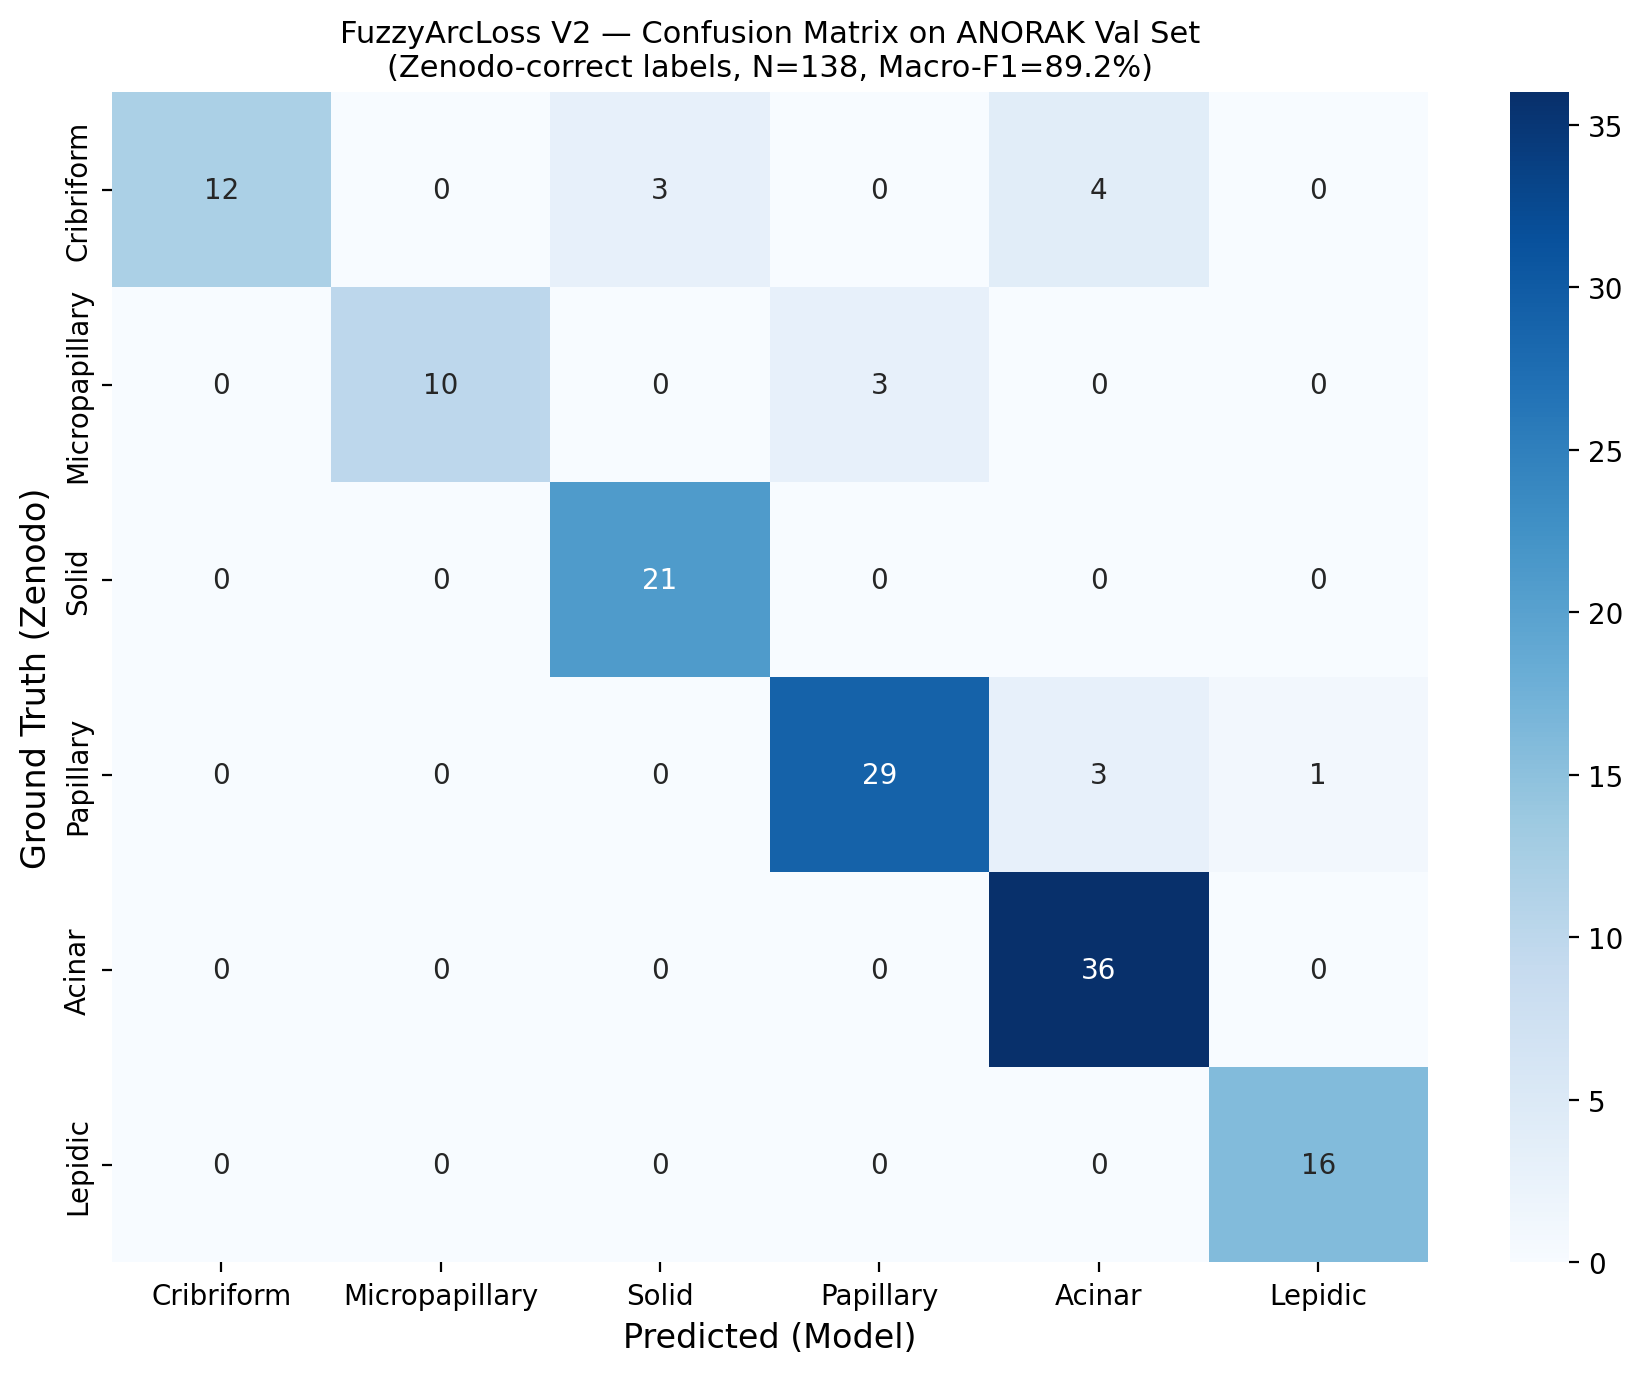
\includegraphics[width=0.75\textwidth]{chapters/figures/confusion_matrix_fuzzyarcloss_v2_zenodo.png}
\caption[Confusion matrix: FuzzyArcLoss V2 on ANORAK validation set]{%
    Confusion matrix for FuzzyArcLoss~V2 on the ANORAK validation set
    (N\,=\,138 tiles).
    Class names follow the corrected Zenodo annotation mapping
    (Table~\ref{tab:variant_types_patterns}).
    Acinar (36/36), solid (21/21), and lepidic (16/16) are perfectly
    classified.
    Cribriform is the most confused class (12/19 correct), primarily
    misclassified as acinar (4~tiles) or solid (3~tiles).
    Micropapillary (10/13 correct) is occasionally confused with
    papillary (3~tiles).}
\label{fig:confusion_matrix}
\end{figure}

Three observations emerge from the confusion matrix:

\begin{enumerate}
    \item \textbf{Acinar, solid, and lepidic are perfectly classified}
    (36/36, 21/21, and 16/16 respectively), indicating that the model
    has learned discriminative features for these morphologically
    distinct patterns.

    \item \textbf{Cribriform is the most confused class} (12/19
    correct; per-class recall\,=\,0.63), primarily misclassified as acinar
    (4~tiles) or solid (3~tiles).
    This is morphologically plausible: cribriform is defined as a
    high-grade acinar variant with sieve-like glandular
    structures~\cite{who2021thoracic}, and its boundary with complex
    acinar and solid patterns is a known source of inter-observer
    disagreement~\cite{thunnissen2012reproducibility}.

    \item \textbf{Micropapillary--papillary confusion} (3~tiles of
    micropapillary classified as papillary; per-class recall\,=\,0.77)
    aligns with the ANORAK paper's finding that micropapillary has the
    lowest inter-observer agreement among pathologists
    ($\rho = 0.35$--$0.44$)~\cite{anorak2024}.
\end{enumerate}

\paragraph{Preliminary expert validation on TCGA slides.}
A board-certified pathologist from SOLCA (Sociedad de Lucha Contra el
C\'{a}ncer del Ecuador) independently reviewed eight subregions from
five TCGA slides processed through LCHAI~v2.0.
Of these, one case (TCGA-49-AAR9, solid-dominant) matched exactly,
and one subregion (acinar) also matched.
However, in five subregions the expert identified \emph{acinar} morphology
where the model predicted \emph{micropapillary}, and in one subregion
the expert found the tissue ``non-assessable'' while the model
predicted micropapillary.

This pattern of disagreement is consistent with two known phenomena:
(i)~\textbf{domain shift} between the ANORAK training cohort
(TRACERx, UK institutions) and the TCGA inference cohort (US
institutions), where differences in scanner hardware, staining
protocols, and tissue preparation may alter the visual features of
pattern boundaries even though both pipelines deliver
$224 \times 224$\,px tiles to the model; and
(ii)~the \textbf{high inter-observer variability of the predicted
class}: in the ANORAK paper~\cite{anorak2024}, micropapillary
shows the lowest pathologist agreement among the six growth patterns
($\rho = 0.35$--$0.44$ across cohorts).
Expert--model disagreements concentrated on exactly this class
(expert: acinar; model: micropapillary): pathologists themselves
disagree about what is and is not micropapillary, so the model's
errors fall on the class with the most ambiguous ground truth.

Critically, this preliminary expert review \emph{does not invalidate}
the tile-level classifier on ANORAK data (where acinar achieves
perfect classification), but highlights that
\textbf{pattern-level predictions on out-of-distribution slides
should be interpreted with caution} and accompanied by pathologist
verification---which is the intended clinical workflow in LCHAI~v2.0.


% ============================================================================
\section{Evaluation of Artifacts 2 and 3: Mutation Prediction}
\label{sec:eval:mutation}
% ============================================================================

This section presents the mutation prediction results for all six experimental
conditions on the LUAD-only cohort (687 slides, 5-fold stratified
cross-validation).

\subsection{Primary Results: LUAD-Only Benchmark}
\label{sec:eval:mutation:luad}

Table~\ref{tab:mutation_luad} reports the AUROC for each (condition, gene) pair.
Results are reported as mean $\pm$ standard deviation across 5 folds.
The highest AUROC per gene is marked in bold.

\begin{table}[ht!]
\centering
\small
\caption{Mutation prediction AUROC (mean $\pm$ std, 5-fold CV) on 687
LUAD-only slides. Best per gene in \textbf{bold}.
B1~=~XGBoost, B2~=~ABMIL embeddings, B3~=~ABMIL patterns,
PI~=~PI-ABMIL (ours), A~=~Ablation one-hot, FC~=~FC-MIL (ours).
Note: PI-ABMIL appears as ``Combined'' in the LCHAI clinical interface.}
\label{tab:mutation_luad}
\begin{tabular}{l c c c c c c c}
\hline
\textbf{Cond.} & \textbf{TP53} & \textbf{EGFR} & \textbf{STK11} &
\textbf{KEAP1} & \textbf{KRAS} & \textbf{RBM10} & \textbf{Mean} \\
\hline
B1  & .518$\pm$.025 & .634$\pm$.033 & .545$\pm$.055 &
      .489$\pm$.034 & .522$\pm$.057 & .474$\pm$.101 & .530 \\
B2  & \textbf{.718}$\pm$.053 & \textbf{.701}$\pm$.049 &
      .684$\pm$.042 & .597$\pm$.081 & .607$\pm$.078 &
      .642$\pm$.054 & .658 \\
B3  & .616$\pm$.043 & .625$\pm$.044 & .617$\pm$.050 &
      .588$\pm$.031 & .545$\pm$.076 & .653$\pm$.081 & .607 \\
PI-ABMIL  & .717$\pm$.058 & .694$\pm$.051 & \textbf{.695}$\pm$.023 &
      \textbf{.610}$\pm$.071 & .590$\pm$.071 & .640$\pm$.064 & .658 \\
A   & .716$\pm$.050 & .695$\pm$.046 & .691$\pm$.050 &
      .594$\pm$.082 & .594$\pm$.071 & .623$\pm$.048 & .652 \\
FC-MIL  & .716$\pm$.047 & .684$\pm$.037 & .658$\pm$.077 &
      .589$\pm$.080 & \textbf{.609}$\pm$.059 &
      \textbf{.661}$\pm$.063 & .653 \\
\hline
\end{tabular}
\end{table}

\begin{figure}[ht!]
\centering
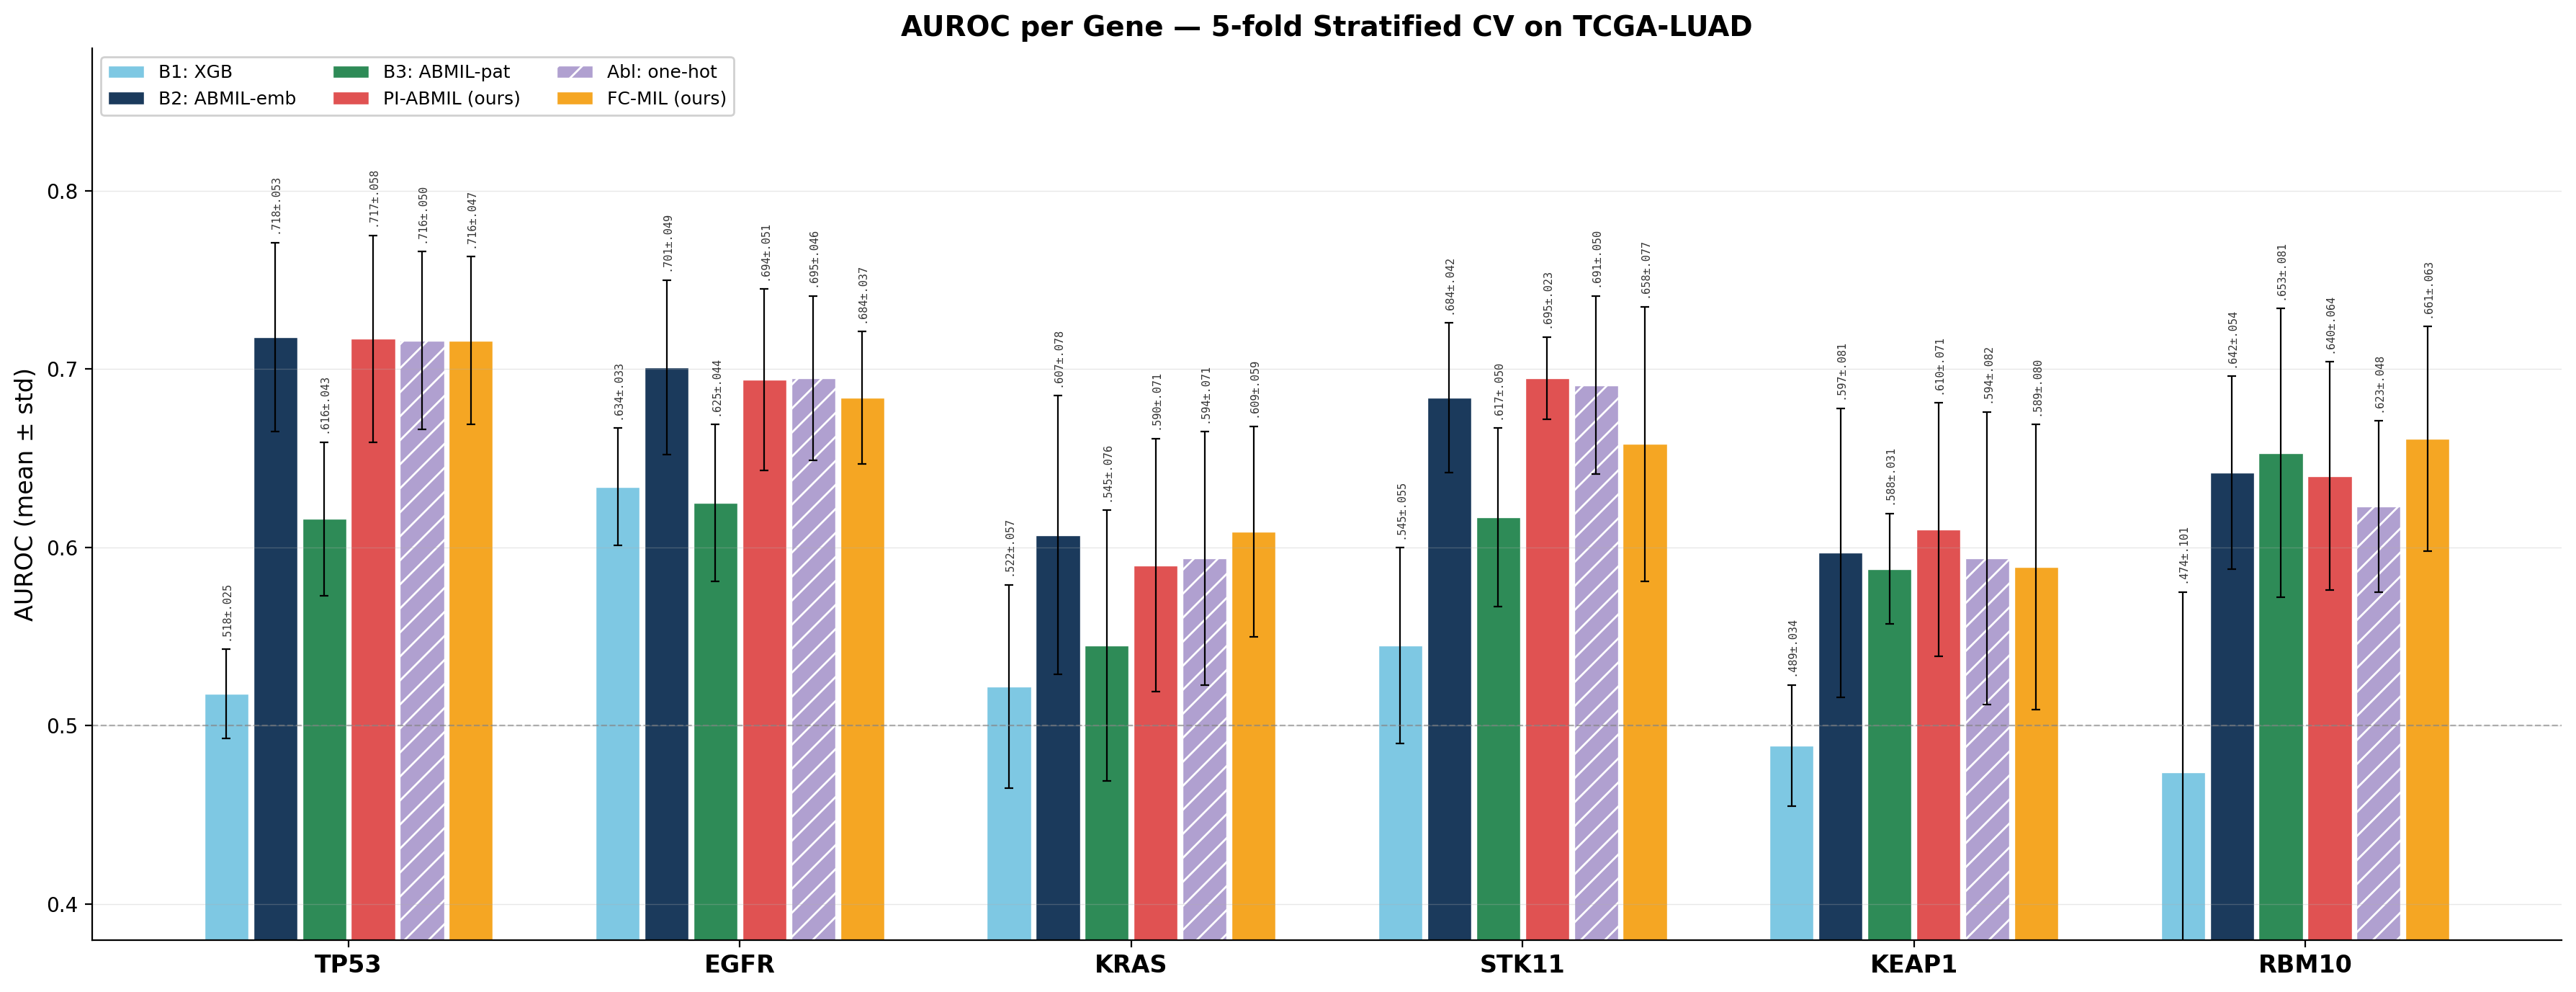
\includegraphics[width=\textwidth]{chapters/figures/auroc_by_gene_ver_15_mar_2026.png}
\caption[AUROC per gene: all six conditions]{%
    PI-ABMIL benchmark results: mean AUROC $\pm$ standard
    deviation per gene across 5-fold patient-stratified cross-validation
    (687 LUAD slides, 668 patients).
    Each panel shows one target gene; bars correspond to the six
    experimental conditions (B1--FC), colour-coded as in the legend
    (B1: light blue, B2: dark blue, B3: green, PI-ABMIL: red,
    Abl one-hot: purple hatched, FC-MIL: orange).
    The dashed horizontal line indicates random performance (AUROC~$= 0.5$).
    The upper-tier conditions (B2, PI-ABMIL, Abl one-hot, FC-MIL)
    perform within $\pm 0.02$ AUROC on TP53, EGFR and STK11, with
    no single dominant winner across genes; PI-ABMIL leads on STK11
    and KEAP1, while FC-MIL leads on KRAS and RBM10
    (cf.~Table~\ref{tab:mutation_luad} for the column-wise maxima).
    High fold-to-fold variance is visible for RBM10 and KEAP1,
    consistent with their low mutation prevalence (5.4\% and 14.3\%
    respectively).}
\label{fig:auroc_by_gene}
\end{figure}

\begin{figure}[ht!]
\centering
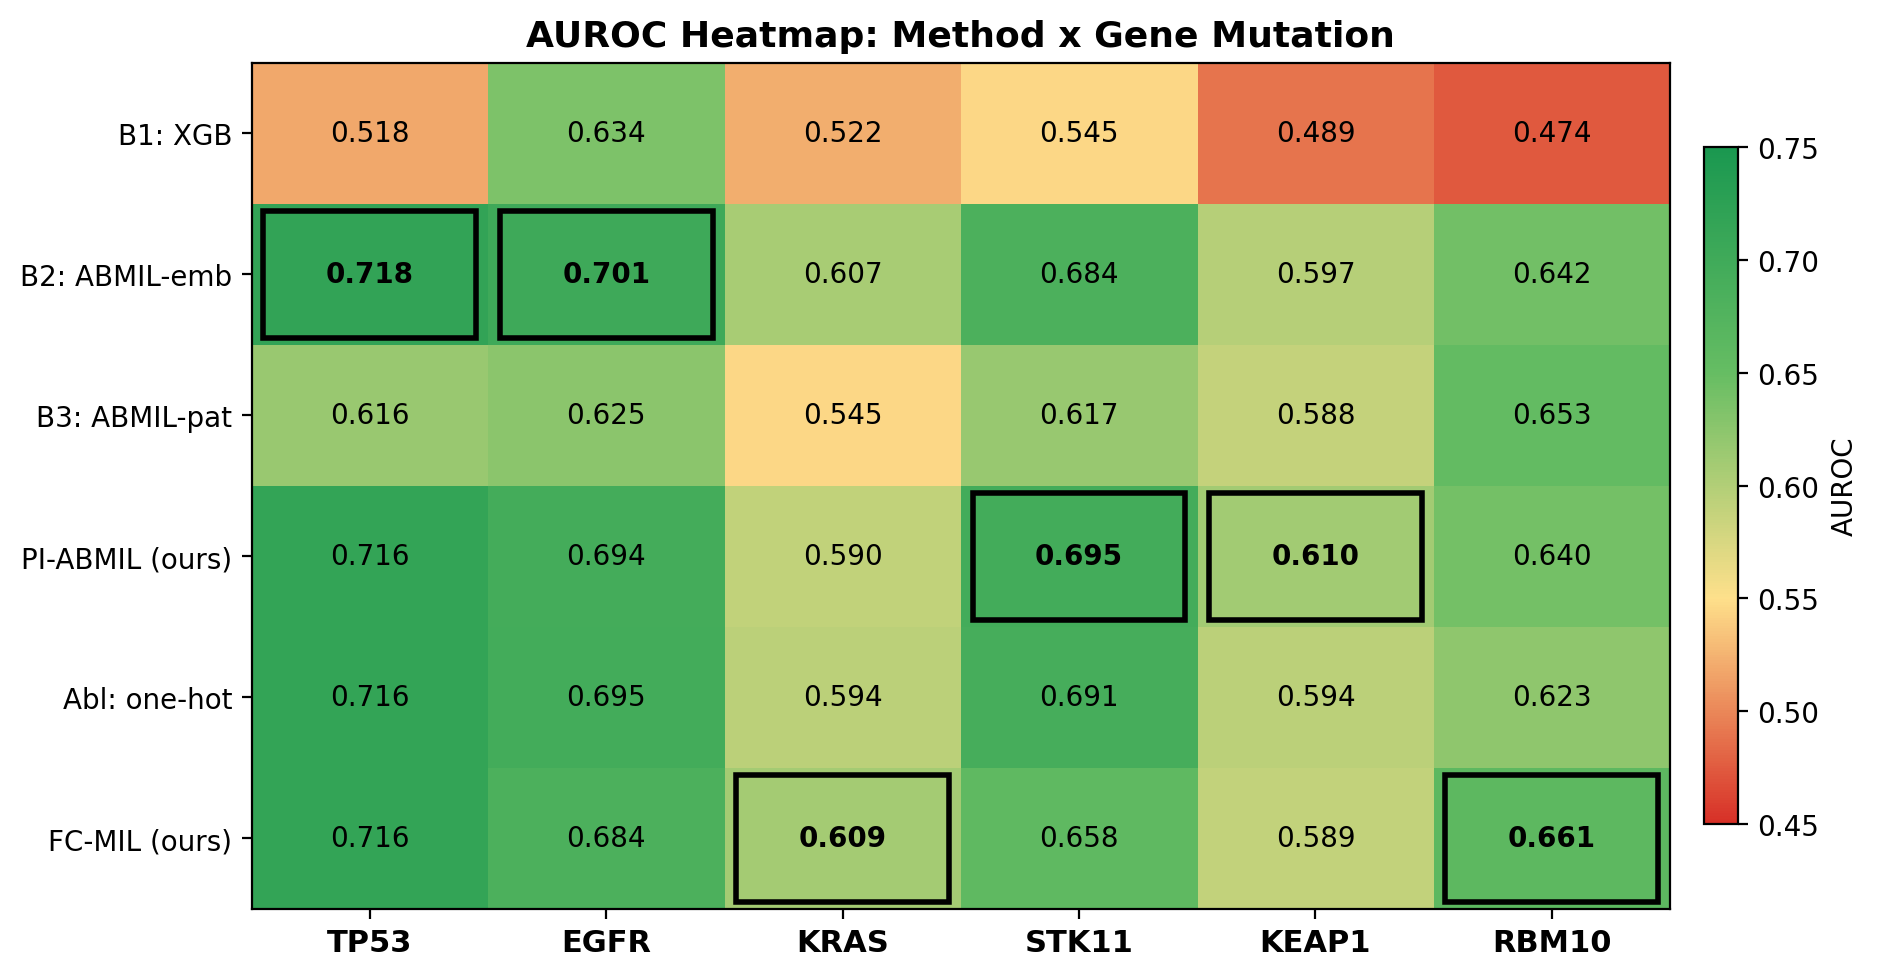
\includegraphics[width=0.85\textwidth]{chapters/figures/auroc_heatmap_ver_15_mar_2026.png}
\caption[AUROC heatmap: condition $\times$ gene]{%
    Mean AUROC heatmap of all 36 (condition, gene) combinations
    (5-fold patient-stratified CV; values in
    Table~\ref{tab:mutation_luad}).
    Colour scale: red~$= 0.50$ (random), yellow-green~$\approx 0.70$,
    dark green~$= 0.90$.
    Bolded cells mark the column-wise (per-gene) maximum.
    Row ordering follows the benchmark hierarchy from the weakest
    condition (B1~XGBoost) to the strongest overall (B2, PI-ABMIL).
    Per-gene leaders are distributed across the upper-tier conditions
    (B2, PI-ABMIL, Abl one-hot, FC-MIL); no single condition dominates
    all six genes. See body text for interpretation.}
\label{fig:auroc_heatmap}
\end{figure}

Figures~\ref{fig:auroc_by_gene}--\ref{fig:auroc_radar} provide
complementary visual summaries of these results.
Figure~\ref{fig:auroc_by_gene} shows the per-gene distribution of
AUROC across conditions with fold-level variance; the heatmap
(Figure~\ref{fig:auroc_heatmap}) enables direct cross-condition and
cross-gene comparison of all 36 mean values simultaneously.
Figure~\ref{fig:auroc_difference} highlights the delta AUROC of each
condition relative to B2 (embedding-only ABMIL), chosen as the
ceiling baseline because it uses the same architecture, encoder, and
training protocol as the proposed methods but without any pattern
information---so the delta isolates the incremental value of domain
knowledge (Section~\ref{sec:meth:mutation:representations}).
Even on the well-predicted genes (TP53, EGFR), the six conditions
split into two clear tiers (Table~\ref{tab:mutation_luad}). The upper
tier---B2, PI-ABMIL, Abl one-hot, and FC-MIL---reaches mean AUROC
within $\pm 0.02$ of one another. The lower tier---B1 and B3---lags
visibly behind: B1 is $0.20$ below B2 on TP53 and $0.07$ below on
EGFR; B3 is $0.10$ below B2 on TP53 and $0.08$ below on EGFR.
The spread between conditions widens further on the difficult genes
(KRAS, STK11, KEAP1, RBM10).
The radar plot (Figure~\ref{fig:auroc_radar}) shows the per-gene
AUROC profile of four key conditions, illustrating that
FC-MIL (FC) expands the profile for KRAS and RBM10 while B2 leads
for TP53 and EGFR.

\begin{figure}[ht!]
\centering
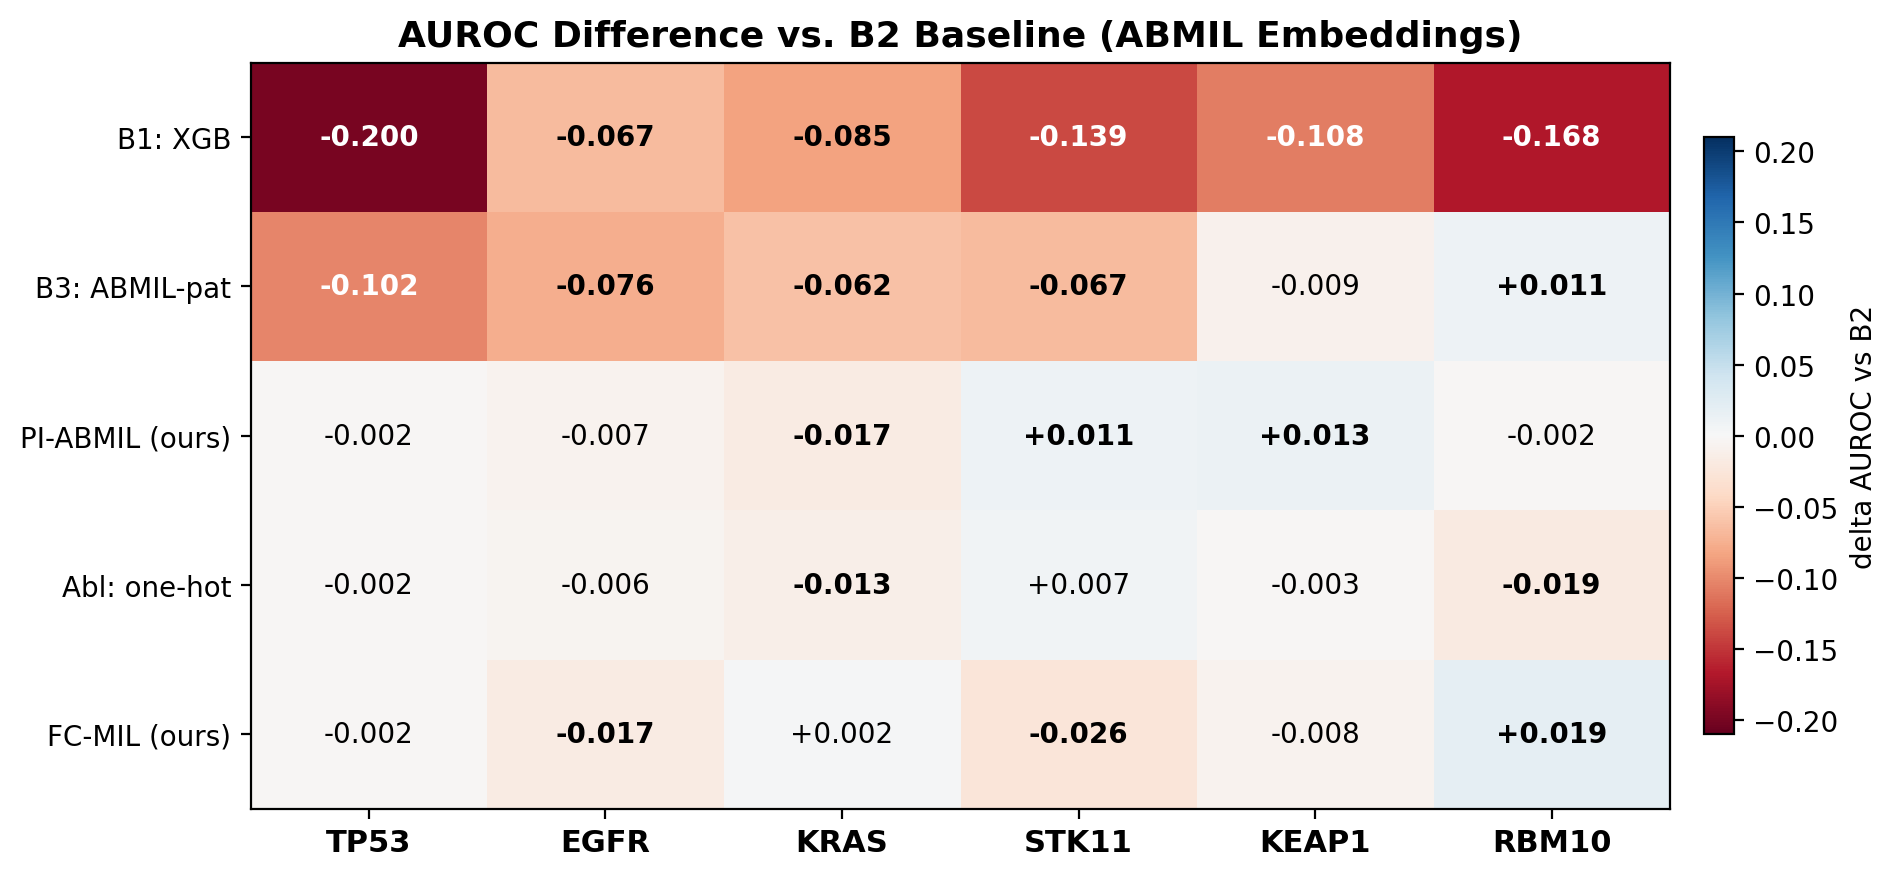
\includegraphics[width=\textwidth]{chapters/figures/auroc_difference_vs_b2.png}
\caption[AUROC difference vs B2 ceiling baseline]{%
    AUROC difference relative to the B2 ceiling baseline (ABMIL embeddings) for
    each (condition, gene) pair.
    Red cells indicate worse performance than B2; blue cells indicate
    improvement.
    B1 (XGBoost) shows the largest deficits across all genes.
    The proposed methods (PI-ABMIL, FC-MIL) show gene-specific improvements:
    FC-MIL gains $+0.019$ for RBM10 and $+0.002$ for KRAS, while PI-ABMIL gains
    $+0.011$ for STK11 and $+0.013$ for KEAP1 (deltas computed from
    Table~\ref{tab:mutation_luad}).}
\label{fig:auroc_difference}
\end{figure}

\begin{figure}[ht!]
\centering
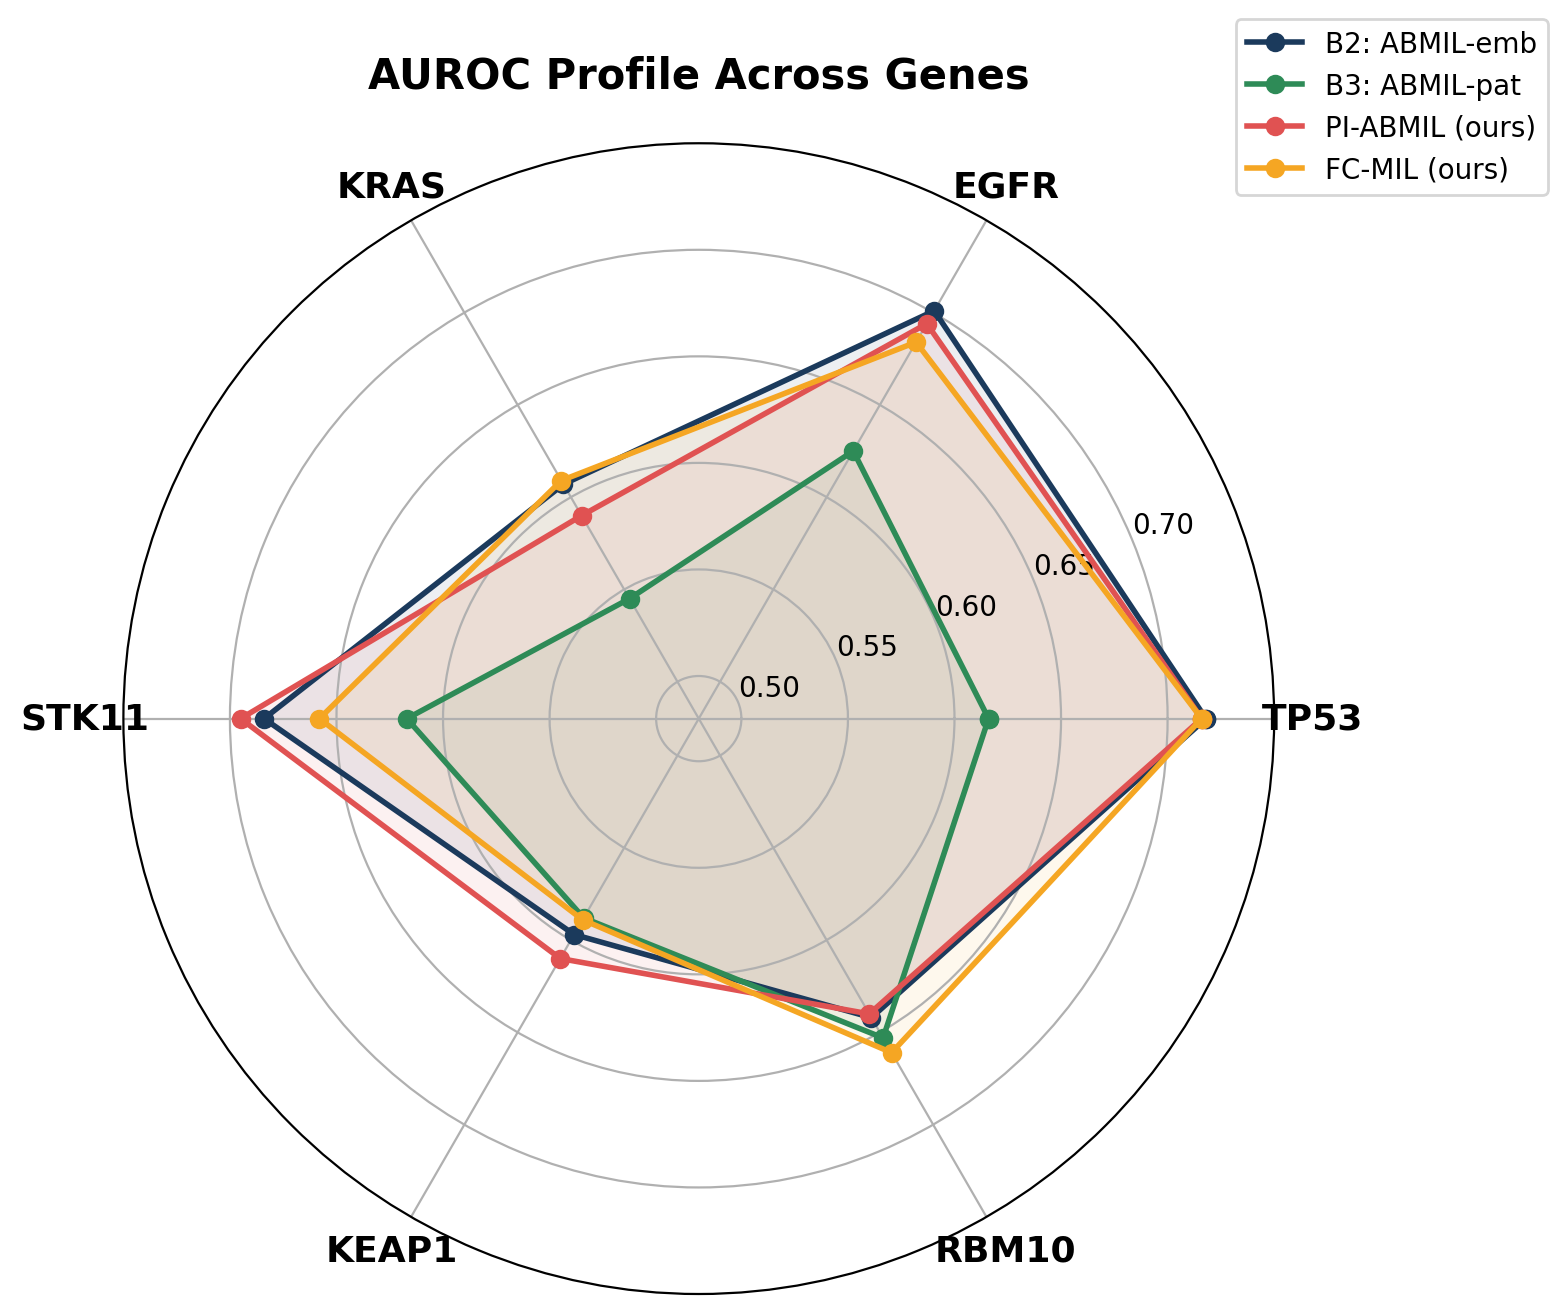
\includegraphics[width=0.7\textwidth]{chapters/figures/auroc_radar_profile.png}
\caption[AUROC radar profile across genes]{%
    Radar plot of mean AUROC across six genes for four conditions:
    B2 (embeddings-only), B3 (patterns-only), PI-ABMIL (ours),
    and FC-MIL (ours).
    B2 and PI-ABMIL nearly overlap for TP53 and EGFR;
    FC-MIL extends the profile for KRAS and RBM10;
    B3 (patterns-only) shows the smallest area, confirming that
    patterns alone are insufficient.}
\label{fig:auroc_radar}
\end{figure}


\begin{figure}[ht!]
\centering
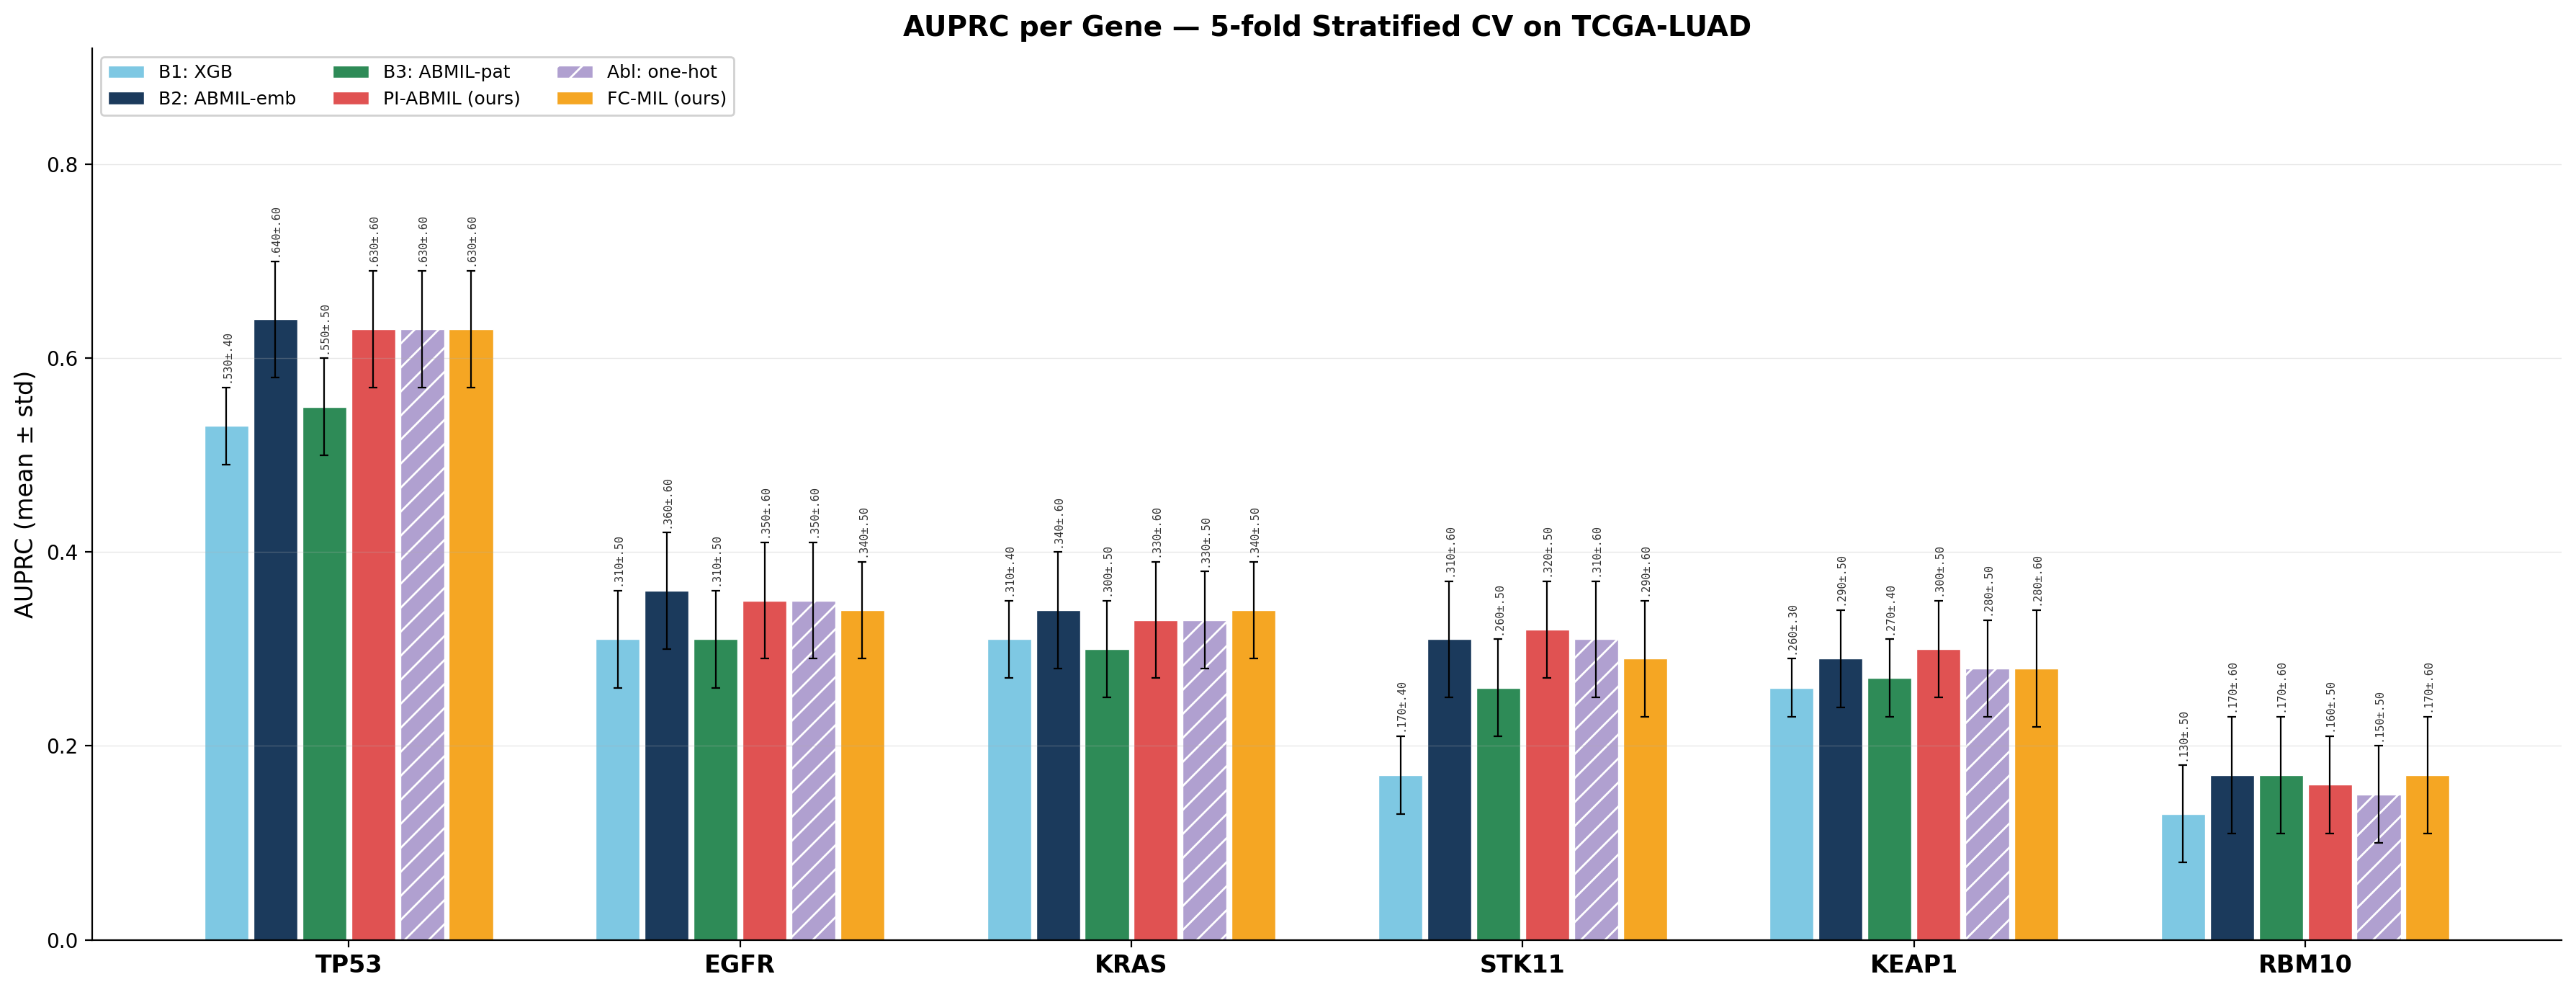
\includegraphics[width=\textwidth]{chapters/figures/auprc_by_gene.png}
\caption[AUPRC per gene: all six conditions]{%
    Area Under the Precision-Recall Curve (AUPRC) per gene for all six
    experimental conditions.
    AUPRC is particularly informative for imbalanced genes: RBM10
    (5.4\% prevalence) and STK11 (9.9\%) show the largest gap between
    AUPRC and AUROC, confirming that high AUROC can coexist with
    modest precision-recall performance when the positive class is rare.
    Error bars show standard deviation across 5 folds.}
\label{fig:auprc_by_gene}
\end{figure}

\paragraph{Complementing AUROC with AUPRC.}
AUROC measures the model's ability to rank positives above negatives
and is invariant to class prevalence. For highly imbalanced binary
problems---as in mutation prediction, where positives range from 5.4\%
(RBM10) to 38.0\% (TP53) of LUAD slides
(Table~\ref{tab:mutation_prevalence})---a high AUROC can coexist with
modest precision-recall performance because most negatives are still
ranked below most positives even when absolute precision at any
clinically useful threshold is low. The Area Under the Precision-Recall
Curve (AUPRC; Figure~\ref{fig:auprc_by_gene}) complements AUROC by
summarising precision across the full range of operating points and is
sensitive to prevalence: its baseline (random classifier) equals the
positive class rate, so AUPRC values must be read in light of each
gene's mutation frequency.
Figure~\ref{fig:auroc_auprc_prevalence} consolidates this relationship
by overlaying, for each gene sorted by ascending mutation prevalence,
the best mean AUROC, the mean AUPRC of that same condition, and the
AUPRC random baseline.

\begin{figure}[ht!]
\centering
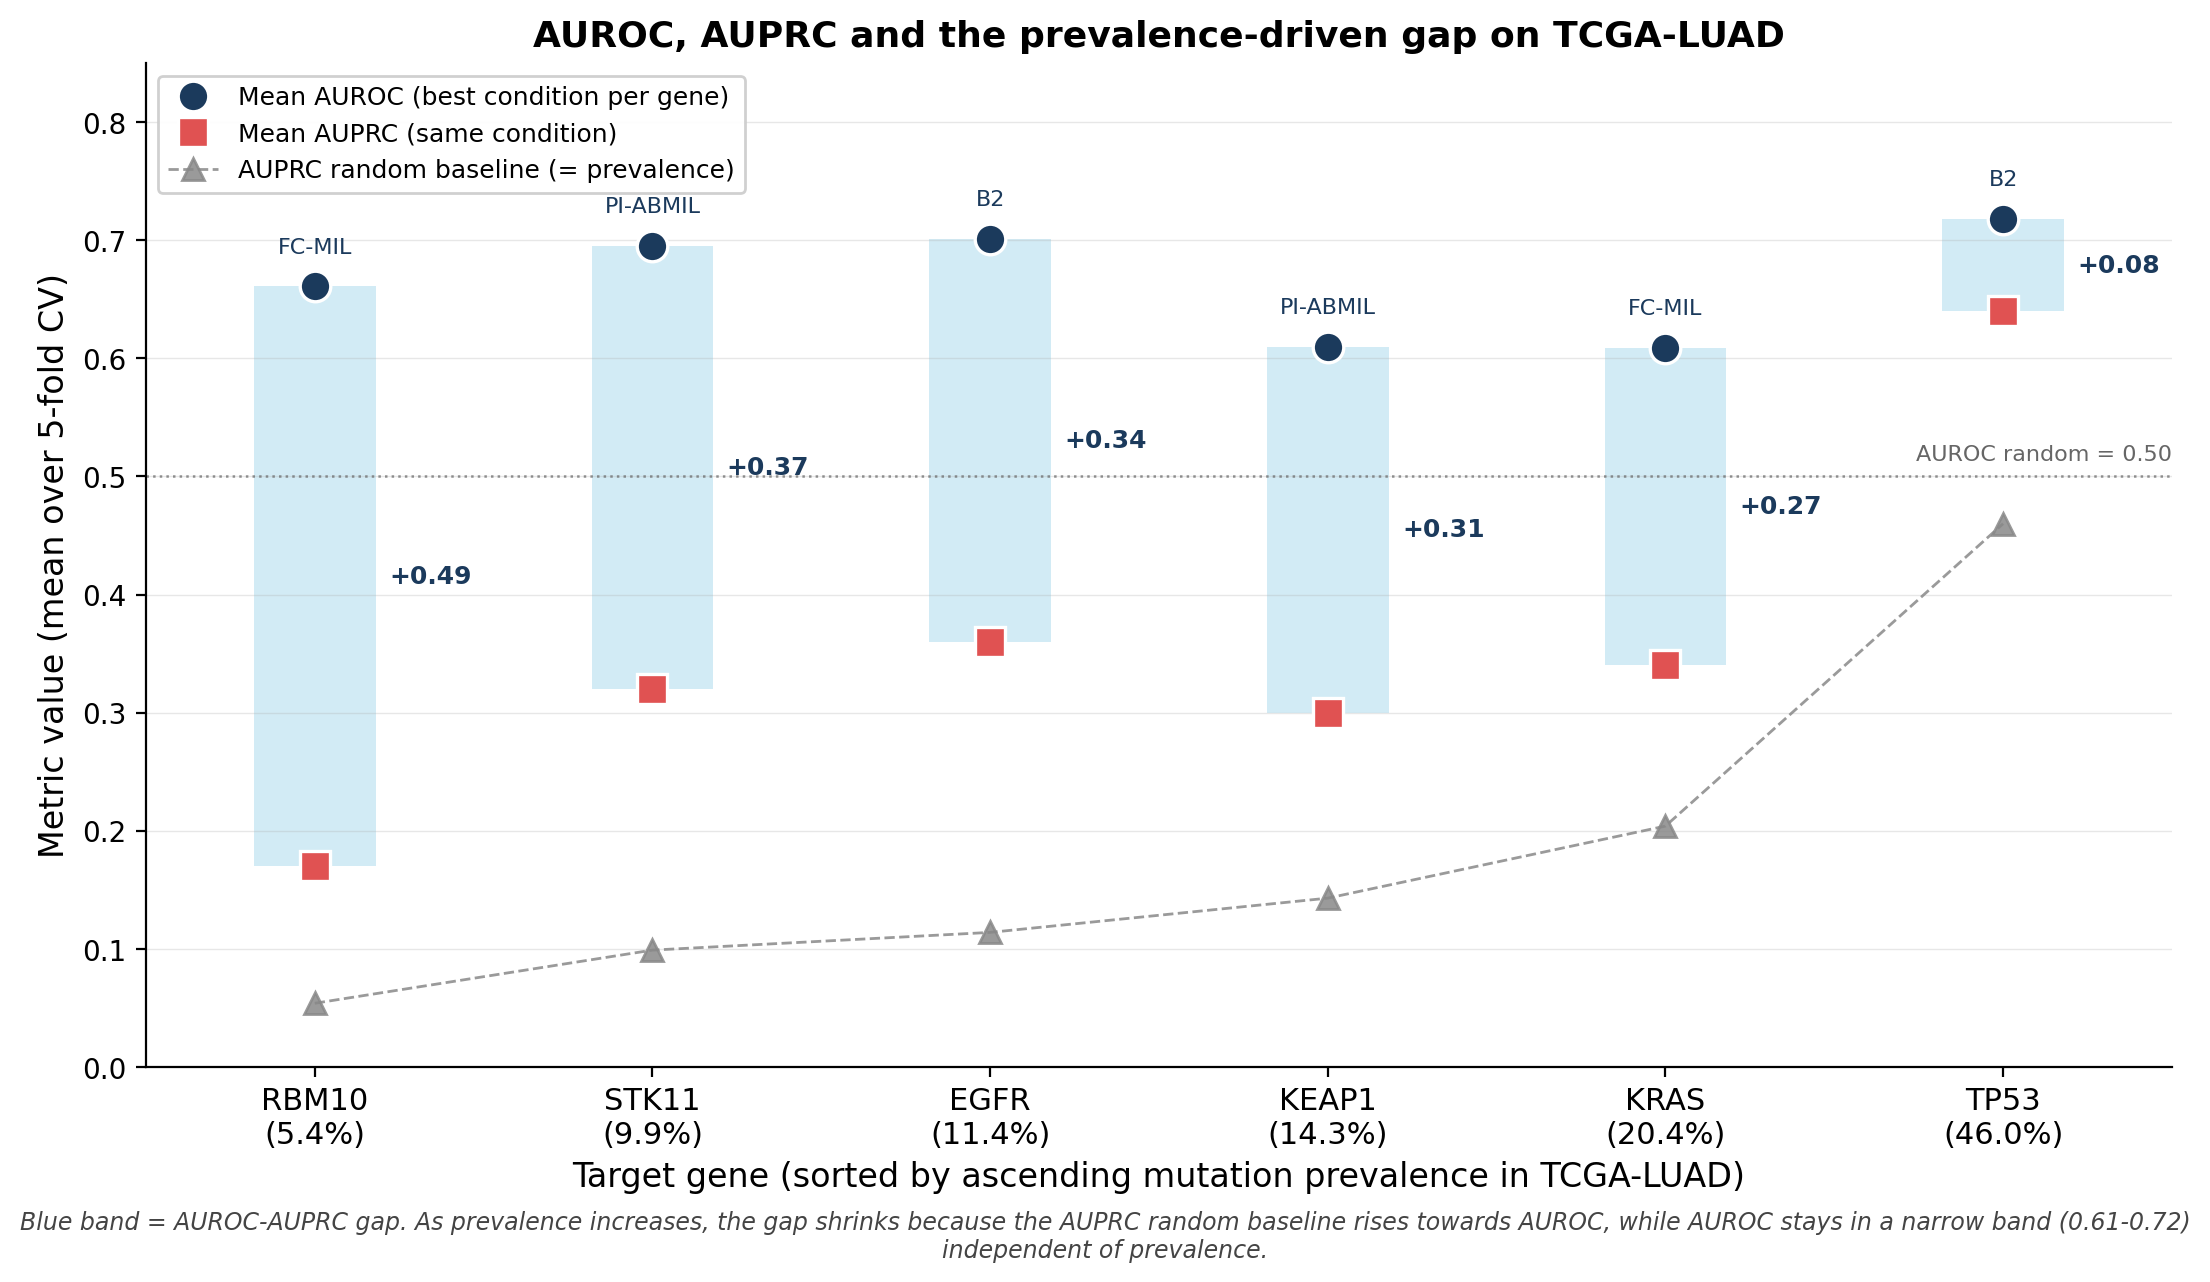
\includegraphics[width=\textwidth]{chapters/figures/auroc_auprc_prevalence.png}
\caption[AUROC, AUPRC and prevalence-driven gap]{%
    Per-gene comparison of mean AUROC and mean AUPRC against
    mutation prevalence in TCGA-LUAD (5-fold CV).
    For each gene the best mean AUROC (dark circle) is plotted with
    the mean AUPRC of the same condition (red square) and the AUPRC
    random baseline equal to the gene's prevalence (gray triangle).
    Genes are sorted by ascending prevalence on the x-axis.
    The shaded blue band marks the AUROC--AUPRC gap and is annotated
    with its numerical value.
    Best AUROC condition is indicated above each circle.
    AUROC stays in a narrow band ($0.61$--$0.72$) regardless of
    prevalence, while AUPRC tracks the random baseline---so the gap
    closes as prevalence rises.
    Values: AUROC column-wise maxima from
    Table~\ref{tab:mutation_luad}; AUPRC values from
    Figure~\ref{fig:auprc_by_gene}.}
\label{fig:auroc_auprc_prevalence}
\end{figure}

\paragraph{Interpreting the AUROC--AUPRC gap.}
The gap between the best mean AUROC and the mean AUPRC of that same
condition per gene (5-fold CV; AUROC column-wise maxima from
Table~\ref{tab:mutation_luad}, AUPRC values from
Figure~\ref{fig:auprc_by_gene}; visual summary in
Figure~\ref{fig:auroc_auprc_prevalence}) correlates inversely with
mutation prevalence.
TP53 (38.0\% prevalence; Table~\ref{tab:mutation_prevalence}) shows
the smallest gap: B2 reaches mean AUROC~0.718 with
mean AUPRC~$\approx$0.64 (gap~$\approx$0.08),
because high prevalence means good ranking translates directly into
acceptable precision-recall.
At the other extreme, RBM10 (5.4\%) shows the largest gap: FC-MIL
reaches mean AUROC~0.661 with mean AUPRC~$\approx$0.17
(gap~$\approx$0.49)---the model ranks reasonably but cannot identify
the rare positives without generating many false positives.
EGFR is a particularly instructive case: B2 is labelled
\emph{Conclusive} on this gene (mean AUROC~0.701~$\geq$~0.70;
Table~\ref{tab:viz_folds}) yet its mean AUPRC is only $\approx$0.36.
Because AUPRC equals the average precision over operating points,
this value implies that at typical decision thresholds the precision
is substantially below 1, with roughly two out of three positive
predictions expected to be false on average.

Two important implications follow:
\begin{enumerate}
    \item \textbf{Method comparisons remain valid in practice.}
    For any given gene, the set of positive slides is \emph{identical}
    across all six experimental conditions---only the model differs,
    not the data---so all methods face the same prevalence-driven
    AUPRC penalty. AUROC and AUPRC are not mathematically
    rank-equivalent (their orderings can diverge under heavy
    imbalance), but in practice the ranking observed under AUROC is
    largely preserved under AUPRC for the six target genes (see
    Figures~\ref{fig:auroc_by_gene} and~\ref{fig:auprc_by_gene}); for
    instance, PI-ABMIL on STK11 maps from AUROC~0.695 to
    AUPRC~$\approx$0.31. Findings~1--6 are based on relative rankings
    (``which method best handles gene $g$?'') rather than absolute
    metric values, and therefore hold under either metric.

    \item \textbf{The Conclusive/Inconclusive threshold may be
    optimistic for moderate-prevalence genes.}
    The current threshold (mean AUROC~$\geq$~0.70) measures
    population-level ranking ability but does not guarantee precision
    at clinically relevant decision thresholds.
    EGFR's AUPRC gap suggests that a composite criterion incorporating
    both AUROC and AUPRC---or a prevalence-adjusted threshold---would
    provide a more conservative and clinically meaningful confidence
    label (see Section~\ref{sec:disc:lim:method} for discussion).
\end{enumerate}

\subsection{Finding 1: Pattern-Informed Approaches Tie the
Embedding-Only Ceiling, and the Tie Hides Three Structural Causes}
\label{sec:eval:mutation:finding1}

The first benchmark question is whether explicitly injecting the
6-dimensional fuzzy pattern vector into the slide-level head moves
the AUROC produced by the same ABMIL backbone running on
CTransPath embeddings alone.
Table~\ref{tab:p_vs_b2} reports the per-gene contrast
PI-ABMIL\,$-$\,B2.

\begin{table}[ht!]
\centering
\caption{Gene-level comparison: PI-ABMIL (PI) versus ABMIL on
CTransPath embeddings only (B2).
$\Delta = \text{PI} - \text{B2}$.}
\label{tab:p_vs_b2}
\begin{tabular}{l c c c}
\hline
\textbf{Gene} & \textbf{B2 (emb)} & \textbf{PI-ABMIL} & \textbf{$\Delta$} \\
\hline
TP53  & 0.718 & 0.717 & $-$0.001 \\
EGFR  & 0.701 & 0.694 & $-$0.007 \\
STK11 & 0.684 & 0.695 & $+$0.011 \\
KEAP1 & 0.597 & 0.610 & $+$0.013 \\
KRAS  & 0.607 & 0.590 & $-$0.017 \\
RBM10 & 0.642 & 0.640 & $-$0.002 \\
\hline
\textbf{Mean} & \textbf{0.658} & \textbf{0.658} & \phantom{$-$}0.000 \\
\hline
\end{tabular}
\end{table}

\textbf{At the cohort mean PI-ABMIL is identical to B2}
($0.658$ vs $0.658$).
Every per-gene delta sits below the $d \approx 1.2$ minimum
detectable effect of a paired test with $K = 5$ folds
(Section~\ref{sec:eval:limitations}); none reaches statistical
significance.
The pretrained encoder neither benefits from nor is harmed by the
auxiliary pattern channel at population level.

\textbf{A uniform tie hides non-uniform structural causes.}
The interesting observation is that the cohort-level tie averages
over genes whose underlying mechanisms are different.
Three structural causes recur throughout the rest of the chapter,
and we name them once here for reuse:
\begin{description}
  \item[(A) Encoder saturation.] The pretrained CTransPath
  embedding ($\mathbb{R}^{512}$, trained on millions of histology
  tiles) already spans the discriminative signal, so adding 6 extra
  hand-engineered dimensions is informationally redundant.
  TP53 ($\Delta = -0.001$) and EGFR ($\Delta = -0.007$) sit in
  this regime.
  \item[(B) Out-of-ontology signal.] The discriminative signal
  exists in the slide but is not expressible within the 6-pattern
  simplex.
  Three distinct sub-mechanisms surface in the per-slide ablation
  and case studies (formalised in
  RQ2(ii), Section~\ref{sec:eval:rq2},
  Figure~\ref{fig:signal_tree}); two of the three names are
  adapted here from established machine-learning terminology and
  one is thesis-specific:
  \emph{label-space mismatch} (STK11 -- the discriminative
  direction lies outside the 6 channels of the schema; the term
  follows the open-set / partial-label-set usage in domain
  adaptation, where the source label set fails to cover the
  target signal~\cite{lipton2018labelshift}),
  \emph{no morphological projection} (KEAP1 -- the signal is not
  in the input modality at all; this name is introduced in this
  thesis and grounded in the established biology of
  KEAP1/NRF2 as an upstream biochemical regulator without a
  robust pattern-level
  correlate~\cite{li2011keap1papillary,tcga2014luad}), and
  \emph{collapse-to-prior} (RBM10 -- no channel departs from the
  base rate at low prevalence; the term parallels
  \emph{posterior collapse} in variational
  inference~\cite{bowman2016posteriorcollapse}, where the
  approximate posterior $q(z|x)$ degenerates to the prior $p(z)$
  and the latent representation carries no information about the
  input).
  STK11 ($\Delta = +0.011$), KEAP1 ($\Delta = +0.013$) and RBM10
  ($\Delta = -0.002$) sit in this regime;
  the cohort lifts on STK11 and KEAP1 are sub-significant
  regularisation noise rather than evidence that patterns recover
  signal, since per-slide ablation contradicts them with
  $\Delta_{\mathrm{pat}} = -5.5$\,pp and $-44.7$\,pp respectively
  (Table~\ref{tab:enrichment_summary}).
  \item[(C) Cross-term in label space.] The signal lives in a
  logical AND of two existing channels and cannot be read by an
  additive head.
  KRAS ($\Delta = -0.017$) is this regime: PI-ABMIL's concatenation
  is the wrong consumer for the right representation, so the pattern
  channel actively hurts unless the head is replaced by a cross-term
  aggregator (Choquet integral; Findings~2 and~4).
\end{description}
Findings~2--6 each make one of these three regimes explicit:
Finding~2 formalises the taxonomy in a single table;
Findings~3--6 show that swapping the encoding (3),
removing the embedding (4), replacing the deep aggregator with
XGBoost (5), or replacing the additive head with Choquet (6) each
produces results that fit the same three-regime structure.

\textbf{Cohort vs.\ per-slide as a diagnostic axis.}
Comparing PI-ABMIL with B2 also defines a per-slide quantity
$\Delta_{\mathrm{pat}}(s) = P_{\mathrm{combined}}(s) -
P_{\mathrm{emb-only}}(s)$, computed slide by slide and surfaced as
Level~5 of the LCHAI~v2.0 interpretability framework
(Section~\ref{sec:eval:interp:enrichment}).
It dissociates feature \emph{attribution} (where the model attends,
what it explains) from predictive \emph{utility} (whether the
pattern channel actually moves the prediction in the right
direction).
On the six representative slides the pattern channel measurably
helps only on KRAS ($+7.6$\,pp) while degrading prediction on
TP53 ($-16.1$\,pp), STK11 ($-5.5$\,pp) and KEAP1 ($-44.7$\,pp), and
is inert on EGFR ($-0.5$\,pp) and RBM10 ($+0.3$\,pp;
Table~\ref{tab:enrichment_summary}).
These per-slide deviations cancel in aggregate, producing the
AUROC tie above; the dissociation is precisely the motivation for
Level~5---when the cohort mean says ``patterns and embeddings are
equivalent'', the per-slide signal still warns the reader whether
the pattern channel is constructive, neutral, or destructive on
the case in front of them.

\subsection{Finding 2: Three Structural Regimes Explain Every
Gene's Optimal Architecture}
\label{sec:eval:mutation:finding2}

The K-fold benchmark stratifies the six target genes by which
architecture wins.
Table~\ref{tab:gene_winners} reads this stratification through the
structural lens introduced in Finding~1: every per-gene win has a
mechanistic cause that determines what kind of intervention---if
any---could improve the result.

\begin{table}[ht!]
\centering
\small
\caption[Best-performing condition per gene on the K-fold
benchmark.]{Best-performing condition per gene on the K-fold
benchmark (LUAD-only, 687 slides; mean AUROC across 5-fold
patient-stratified cross-validation, from
Table~\ref{tab:mutation_luad}).
The \emph{Mechanism} column reflects the underlying cause of each
gene's ranking once Finding~1, RQ2(ii)
(Section~\ref{sec:eval:rq2}, Figure~\ref{fig:signal_tree}) and the
per-slide ablation
(Table~\ref{tab:enrichment_summary}) are read together; for
STK11, KEAP1 and RBM10 the cohort-mean lift is sub-significant
($\Delta < d \approx 1.2$ MDE with $K = 5$ folds) and is best
interpreted via the ontology-coverage taxonomy rather than as a
positive contribution of the pattern channel.}
\label{tab:gene_winners}
\begin{tabular}{l l c p{6.4cm}}
\hline
\textbf{Gene} & \textbf{Best condition} & \textbf{Mean AUROC} &
\textbf{Mechanism} \\
\hline
TP53  & B2 (embeddings) & 0.718 &
  CTransPath embedding saturates the morphological signal \\
EGFR  & B2 (embeddings) & 0.701 &
  CTransPath embedding saturates the morphological signal \\
STK11 & PI-ABMIL (ours) & 0.695 &
  Cohort-mean tie within fold variance; per-slide
  $\Delta_{\mathrm{pat}} = -5.5$\,pp (label-space mismatch:
  signal in TME outside ANORAK simplex) \\
KEAP1 & PI-ABMIL (ours) & 0.610 &
  Cohort-mean tie within fold variance; per-slide
  $\Delta_{\mathrm{pat}} = -44.7$\,pp (no morphological
  projection: biochemical regulator) \\
KRAS  & FC-MIL (ours)   & 0.609 &
  Genuine inter-pattern interaction:
  $I_{\,\mathrm{lepidic, solid}} = +0.032$ proxies the missing
  invasive mucinous class \\
RBM10 & FC-MIL (ours)   & 0.661 &
  Architectural negative control: Choquet branch empty
  (singleton spread $0.0007$, all $|I| < 0.01$); lift originates
  in the shared embedding pathway \\
\hline
\end{tabular}
\end{table}

\paragraph{How the recasting was performed.}
\label{par:eval:regime_decision_rules}
Each gene's empirical result is classified into one of the three
regimes by triangulating four pre-specified evidence sources, all
already reported in this chapter:
(i)~\textbf{cohort-mean AUROC across conditions}
(B2 vs.\ PI-ABMIL vs.\ A vs.\ FC-MIL,
Table~\ref{tab:mutation_luad}),
which exposes whether any explicit pattern channel adds discriminative
signal at the cohort level;
(ii)~\textbf{minimum detectable effect (MDE) under $K=5$ folds}
($d \approx 1.2$, derived in
Section~\ref{sec:eval:lim:design}), which separates real lifts from
noise---any cohort lift below the MDE is treated as a null observation
rather than a positive contribution;
(iii)~\textbf{per-slide ablation $\Delta_{\mathrm{pat}}$ on the
representative case} (Table~\ref{tab:enrichment_summary}), which tests
whether the pattern channel matters \emph{at the prediction level} on
real cases, not just on average across folds;
and (iv)~\textbf{FC-MIL Choquet engagement}
(singleton spread and pairwise interaction indices
$I_{kl}$, Section~\ref{sec:eval:interp:choquet}), which tests
whether the model has discovered non-trivial pattern interactions or
its second branch is silent.
The decision rules that follow from these sources are:
\begin{itemize}
  \item \textbf{Regime~A} (encoder saturation) is assigned when
  cohort AUROC is statistically tied across all conditions
  ($\Delta < $ MDE) \emph{and} per-slide $\Delta_{\mathrm{pat}}$ on
  the representative case is not negative.
  The pattern channel provides neither cohort-level nor per-slide
  marginal value; the signal is already in the embedding.
  \item \textbf{Regime~B} (out-of-ontology signal) is assigned when
  cohort lifts are sub-significant ($\Delta < $ MDE) \emph{and} the
  per-slide ablation shows a negative or null
  $\Delta_{\mathrm{pat}}$, indicating the pattern channel actively
  fails to recover signal on real cases.
  Three sub-mechanisms (label-space mismatch / no morphological
  projection / collapse-to-prior) are distinguished by domain
  evidence and developed gene-by-gene in the Regime~B paragraph
  below.
  \item \textbf{Regime~C} (cross-term in label space) is assigned
  when PI-ABMIL collapses (linear concatenation cannot represent the
  pattern AND-conjunction) \emph{but} FC-MIL recovers leading AUROC
  \emph{and} learns a non-trivial pairwise interaction
  $|I_{kl}|$ above the noise floor of the singleton spread.
  Both conditions must hold: a Choquet branch that is empty
  (singleton spread $< 0.001$, all $|I_{kl}| < 0.01$) is treated as
  Regime~B with an architectural negative-control reading rather
  than as Regime~C---this is exactly what RBM10 exhibits
  (Section~\ref{sec:eval:interp:choquet}).
\end{itemize}
The same decision rules apply to any new gene added to the panel,
making the classification a reproducible procedure rather than a
post-hoc narrative.

\paragraph{Regime A --- encoder saturation (TP53, EGFR).}
The pretrained CTransPath embedding has been trained on millions of
histology tiles and already encodes the dominant morphological
correlates these mutations express
(TP53~\cite{ahn2022tp53highgrade},
EGFR~\cite{yoshizawa2013egfrmorph}).
The hand-engineered 6-dimensional pattern vector is a strict subset
of what the embedding already captures, so concatenation cannot
add discriminative information.
Both genes' AUROC sits within fold variance regardless of whether
the pattern channel is concatenated, dropped, or one-hot-encoded
(Table~\ref{tab:p_vs_b2}; Findings~3,~6).
The white-box pattern channel still carries interpretive value
through the LCHAI overlay (Level~2 of the framework,
Section~\ref{sec:eval:interp:attention}), but no marginal
discriminative one.

\paragraph{Regime B --- out-of-ontology signal (STK11, KEAP1,
RBM10).}
For these genes the discriminative signal is \emph{not present}
within the 6-pattern simplex.
Three distinct sub-mechanisms surface in the per-slide ablation
(Table~\ref{tab:enrichment_summary}) and are formalised in RQ2(ii)
(Section~\ref{sec:eval:rq2}, Figure~\ref{fig:signal_tree}) as the
ontology-coverage taxonomy:

\begin{itemize}
  \item \emph{Label-space mismatch} (STK11). The signal exists in
  the slide but lives in the tumour microenvironment---specifically,
  in the density and spatial distribution of immune cells
  infiltrating the
  tumour~\cite{skoulidis2018stk11pd1,pineda2025stk11morphology}.
  The ANORAK ontology was designed to label \emph{how tumour cells
  are arranged geometrically} (six layouts), not \emph{who is around
  them}.
  In representational terms, the schema does not contain a basis
  vector aligned with the discriminative direction; this is a
  feature-engineering problem rather than an architectural one.

  \item \emph{No morphological projection} (KEAP1).
  KEAP1 regulates the NRF2 oxidative-stress
  pathway~\cite{li2011keap1papillary,tcga2014luad}---a biochemical
  function with no robust visible correlate at H\&E resolution.
  The signal is not in the input modality at all; histology is a
  render of tissue architecture and does not capture biochemistry.
  No model trained on H\&E alone can recover what the input does
  not contain.

  \item \emph{Collapse-to-prior} (RBM10).
  Per-slide ablation shows every channel---combined, embedding-only,
  pattern-only---failing to depart from the prevalence
  ($P(\mathrm{mut}) \approx 0.054$) on the representative case
  (Figure~\ref{fig:rbm10_cleanest_null}).
  At 5.4\% prevalence (37 mutated slides out of 687) the model has
  too few positive examples to find a stable signature in any of
  the three feature streams.
\end{itemize}
The cohort-mean lifts that PI-ABMIL claims for STK11 ($+0.011$)
and KEAP1 ($+0.013$), and that FC-MIL claims for RBM10
($+0.026$), all fall below the $d \approx 1.2$ MDE bound and are
contradicted at slide level by negative or null
$\Delta_{\mathrm{pat}}$ (Table~\ref{tab:enrichment_summary}).
They are best read as small regularising or shared-pathway
artefacts rather than as evidence that the pattern channel
recovers signal in this regime
(quantitative breakdown in Findings~3 and~6).

\paragraph{Regime C --- cross-term in label space (KRAS).}
This is the only gene where the pattern channel carries genuine
signal that the embedding pathway does not already exploit.
KRAS-driven invasive mucinous adenocarcinoma (IMA) is a tumour
type the WHO~2021 classification recognises~\cite{who2021thoracic}
but the ANORAK ontology does not include as an explicit category;
its architectural signature is documented in the literature as a
co-presence of \emph{lepidic} growth (tumour cells creeping along
existing lung surfaces) with one or more non-lepidic patterns
(typically \emph{solid}) plus abundant
mucus~\cite{cha2017imapatterns,hwang2017nonlepidicima,shim2015krasmucinous,rekhtman2013krassolid}
(Figure~\ref{fig:kras_lepidic_solid_proxy}, left panel).
The 6-pattern schema has no mucinous channel because mucus is
something the cells \emph{contain}, not the way they are arranged
(Section~\ref{sec:uc:luad_histology}; centre panel of the figure),
so the property that most directly distinguishes IMA is
unrepresentable as a single basis vector.
The schema can still encode IMA, however, as a logical AND of two
existing channels: \emph{lepidic} and \emph{solid} both fire on
the same slide.
A linear-concatenation head (PI-ABMIL) cannot represent this AND
($w_l p_l + w_s p_s \neq p_l \cdot p_s$), so PI-ABMIL collapses on
KRAS ($\Delta = -0.017$ vs.\ B2; Table~\ref{tab:p_vs_b2}).
FC-MIL's Choquet integral, which has 15 trainable pairwise
interaction indices in addition to 6 singleton Shapley values,
learns $I_{\,\mathrm{lepidic,\,solid}} = +0.032$---the largest of
the 15 pairs---and recovers the top KRAS AUROC ($0.609$;
Section~\ref{sec:eval:interp:choquet}, bottom panel of
Figure~\ref{fig:kras_lepidic_solid_proxy}).
This is the only case in the thesis where a pattern interaction
recovers discriminative signal that no embedding-only architecture
extracts; the architectural consequences (and how the same
mechanism explains the B3 and B1 ablations) are detailed in
Finding~4 (Section~\ref{sec:eval:mutation:finding4},
Figure~\ref{fig:kras_two_routes}).

\begin{figure}[ht!]
  \centering
  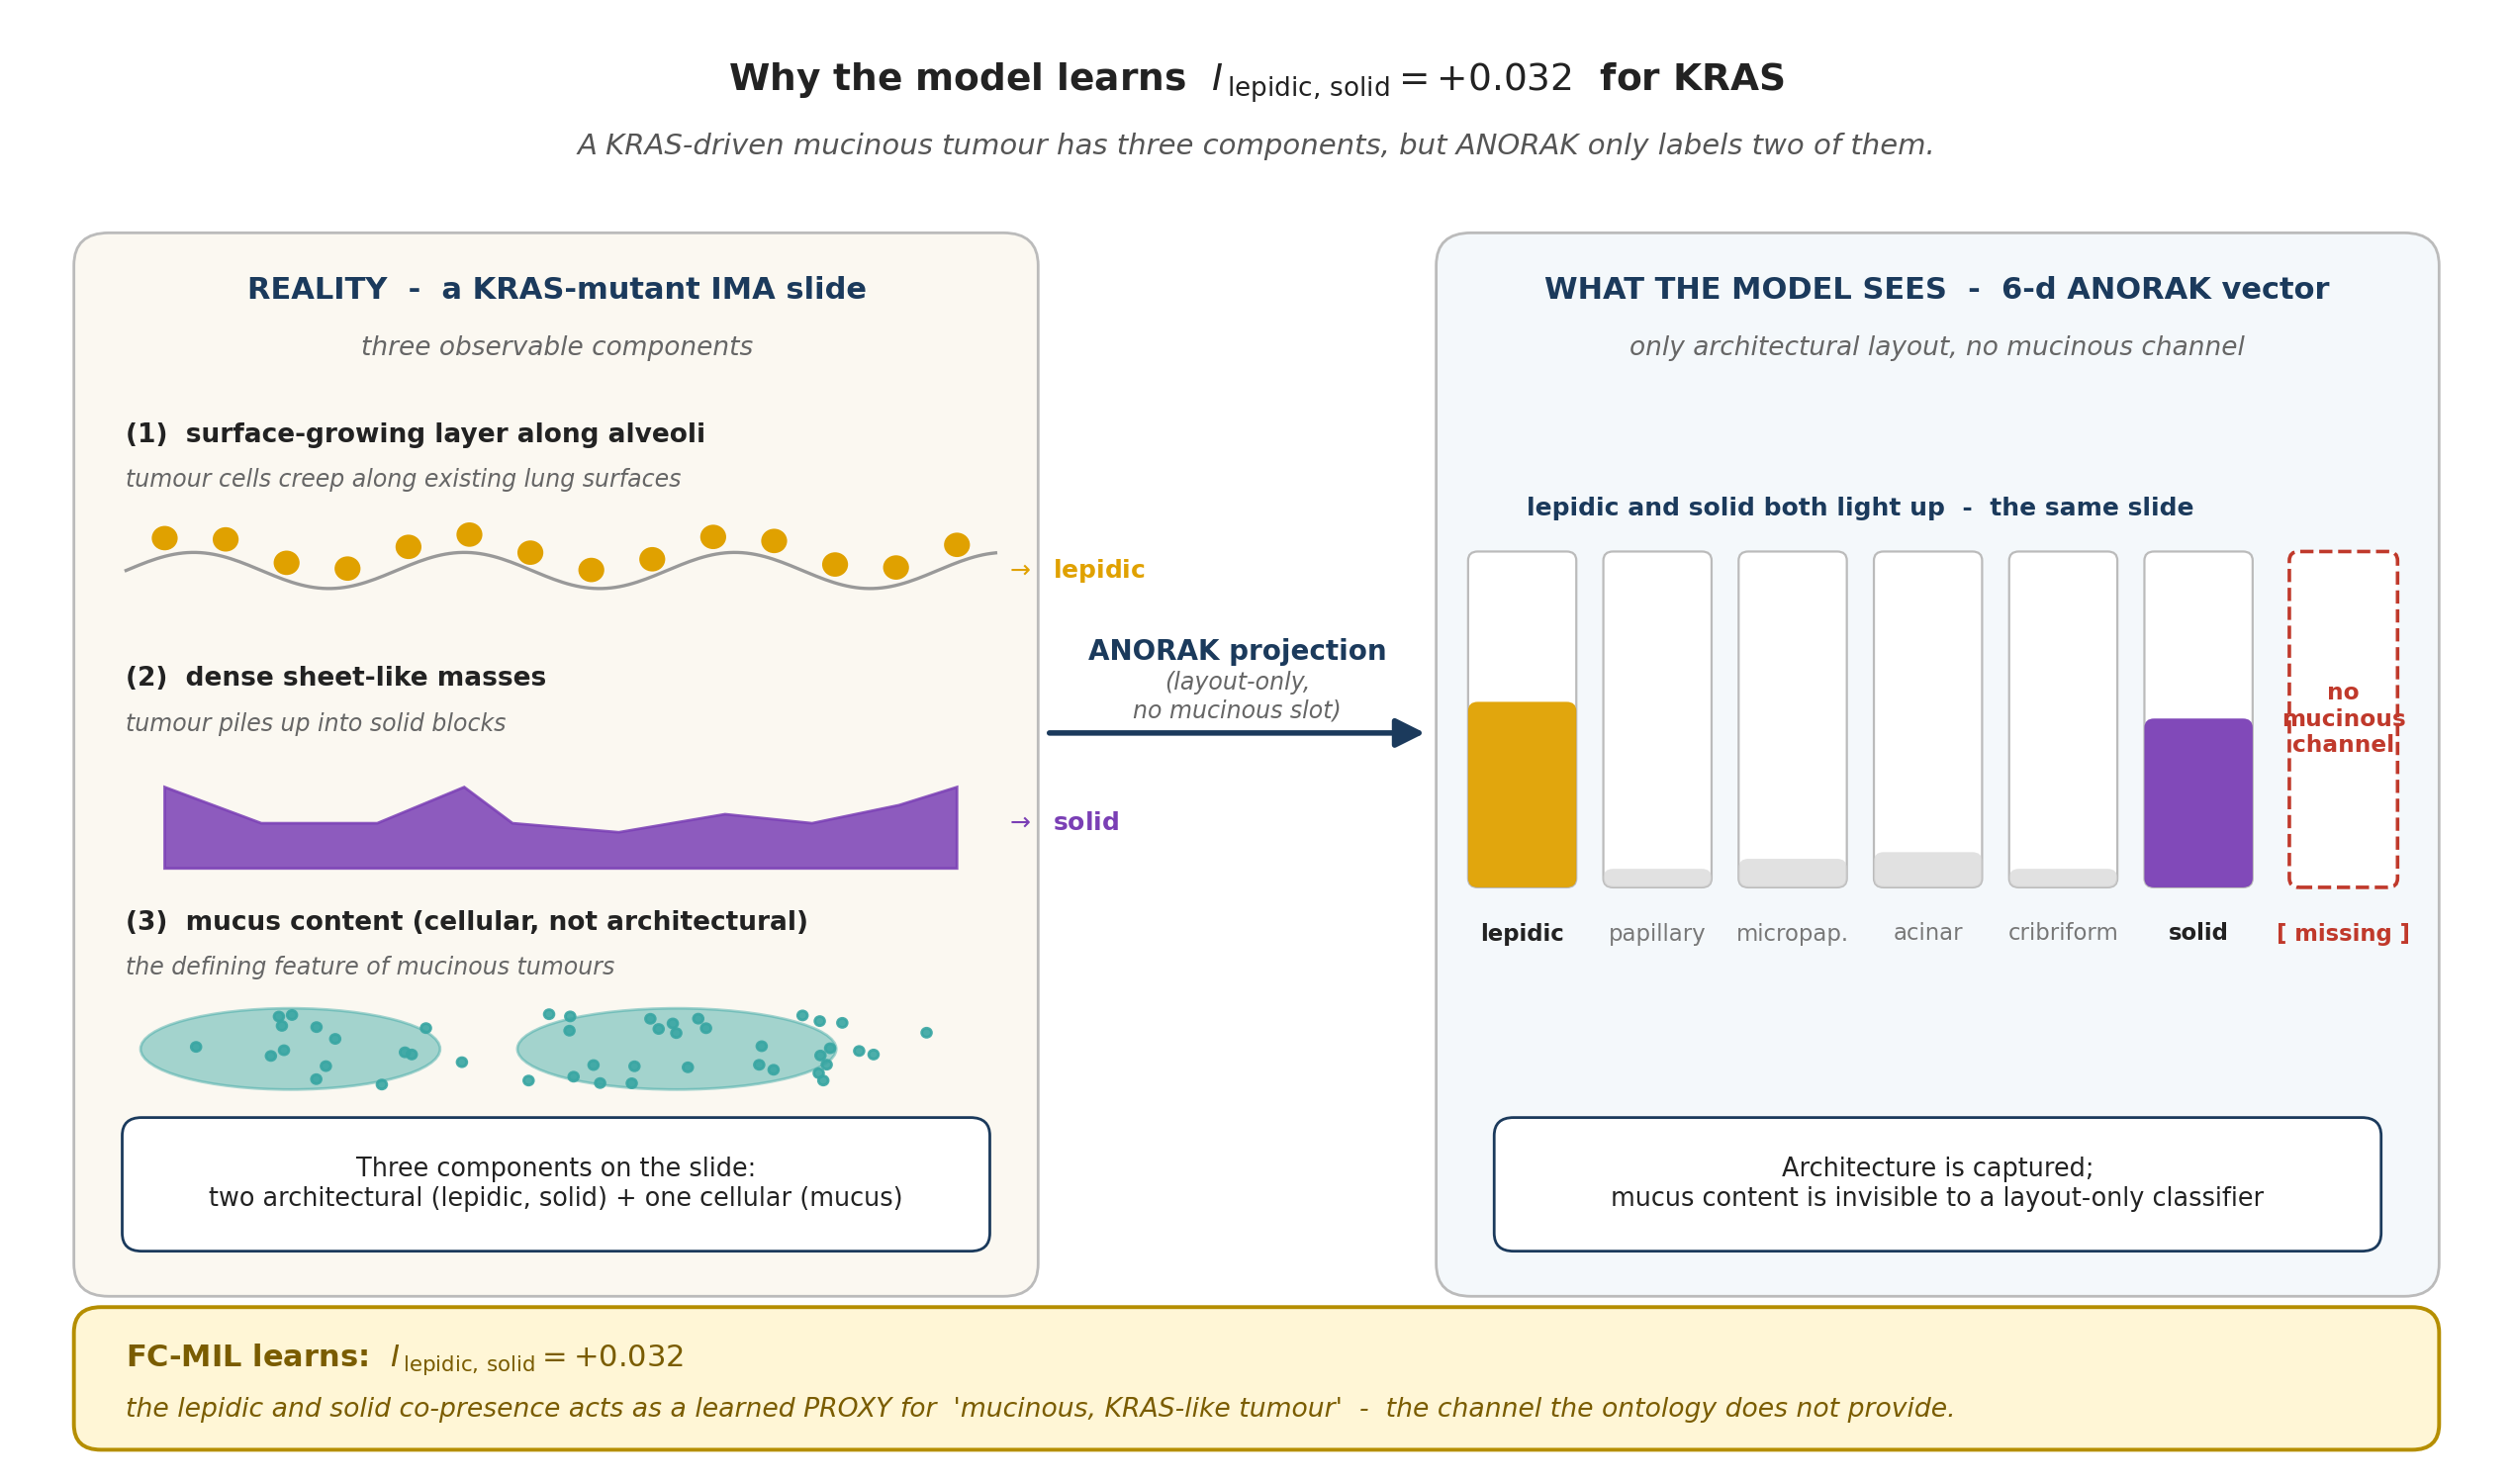
\includegraphics[width=\textwidth]{chapters/figures/kras_lepidic_solid_proxy.png}
  \caption[Why FC-MIL learns
    $I_{\,\mathrm{lepidic,\,solid}} = +0.032$ for KRAS]{%
    Why FC-MIL learns
    $I_{\,\mathrm{lepidic,\,solid}} = +0.032$ for KRAS.
    A KRAS-mutant invasive mucinous adenocarcinoma (IMA) shows a
    mixed lepidic\,$+$\,non-lepidic (often solid) architecture plus
    abundant mucus
    (left)~\cite{who2021thoracic,cha2017imapatterns,hwang2017nonlepidicima,shim2015krasmucinous,rekhtman2013krassolid},
    but ANORAK's six-channel layout ontology has no mucinous
    channel (right; Section~\ref{sec:uc:luad_histology}).
    FC-MIL therefore encodes IMA as a lepidic--solid co-presence
    (bottom; Table~\ref{tab:choquet_interactions}); strictly, this
    pair is not unique to IMA, but on top of a KRAS-supervised loss
    it is the most discriminative proxy available within the
    six-channel layout ontology.}
  \label{fig:kras_lepidic_solid_proxy}
\end{figure}

\paragraph{Why this is a structural finding rather than a method
preference.}
The three regimes classify each gene by \emph{the kind of problem}
its mutation prediction poses, not by \emph{which model happens to
win}.
That distinction is actionable: regime A cannot be improved by
adding more handcrafted features at inference (the encoder is
already saturated; gains require pretraining on more data or a
better objective);
regime B is fixed only by changing inputs---extending the ontology
for label-space mismatch (STK11), adding a different modality for
the no-morphological-projection case (KEAP1; e.g.\ multi-omics
fusion), or acquiring more positive examples for collapse-to-prior
(RBM10);
regime C is fixed by replacing the additive head with a cross-term
aggregator, which is exactly what FC-MIL's Choquet integral does
(Finding~6, Section~\ref{sec:eval:mutation:finding6}).
The taxonomy is therefore the \emph{ontology-coverage}
contribution of the thesis (RQ2(ii), Section~\ref{sec:eval:rq2}):
independent of any specific architecture, it bounds what
morphology-only mutation prediction on the ANORAK simplex can
achieve.
Figure~\ref{fig:signal_tree} consolidates the three regimes and
their gene assignments in a single view.

\begin{figure}[ht!]
\centering
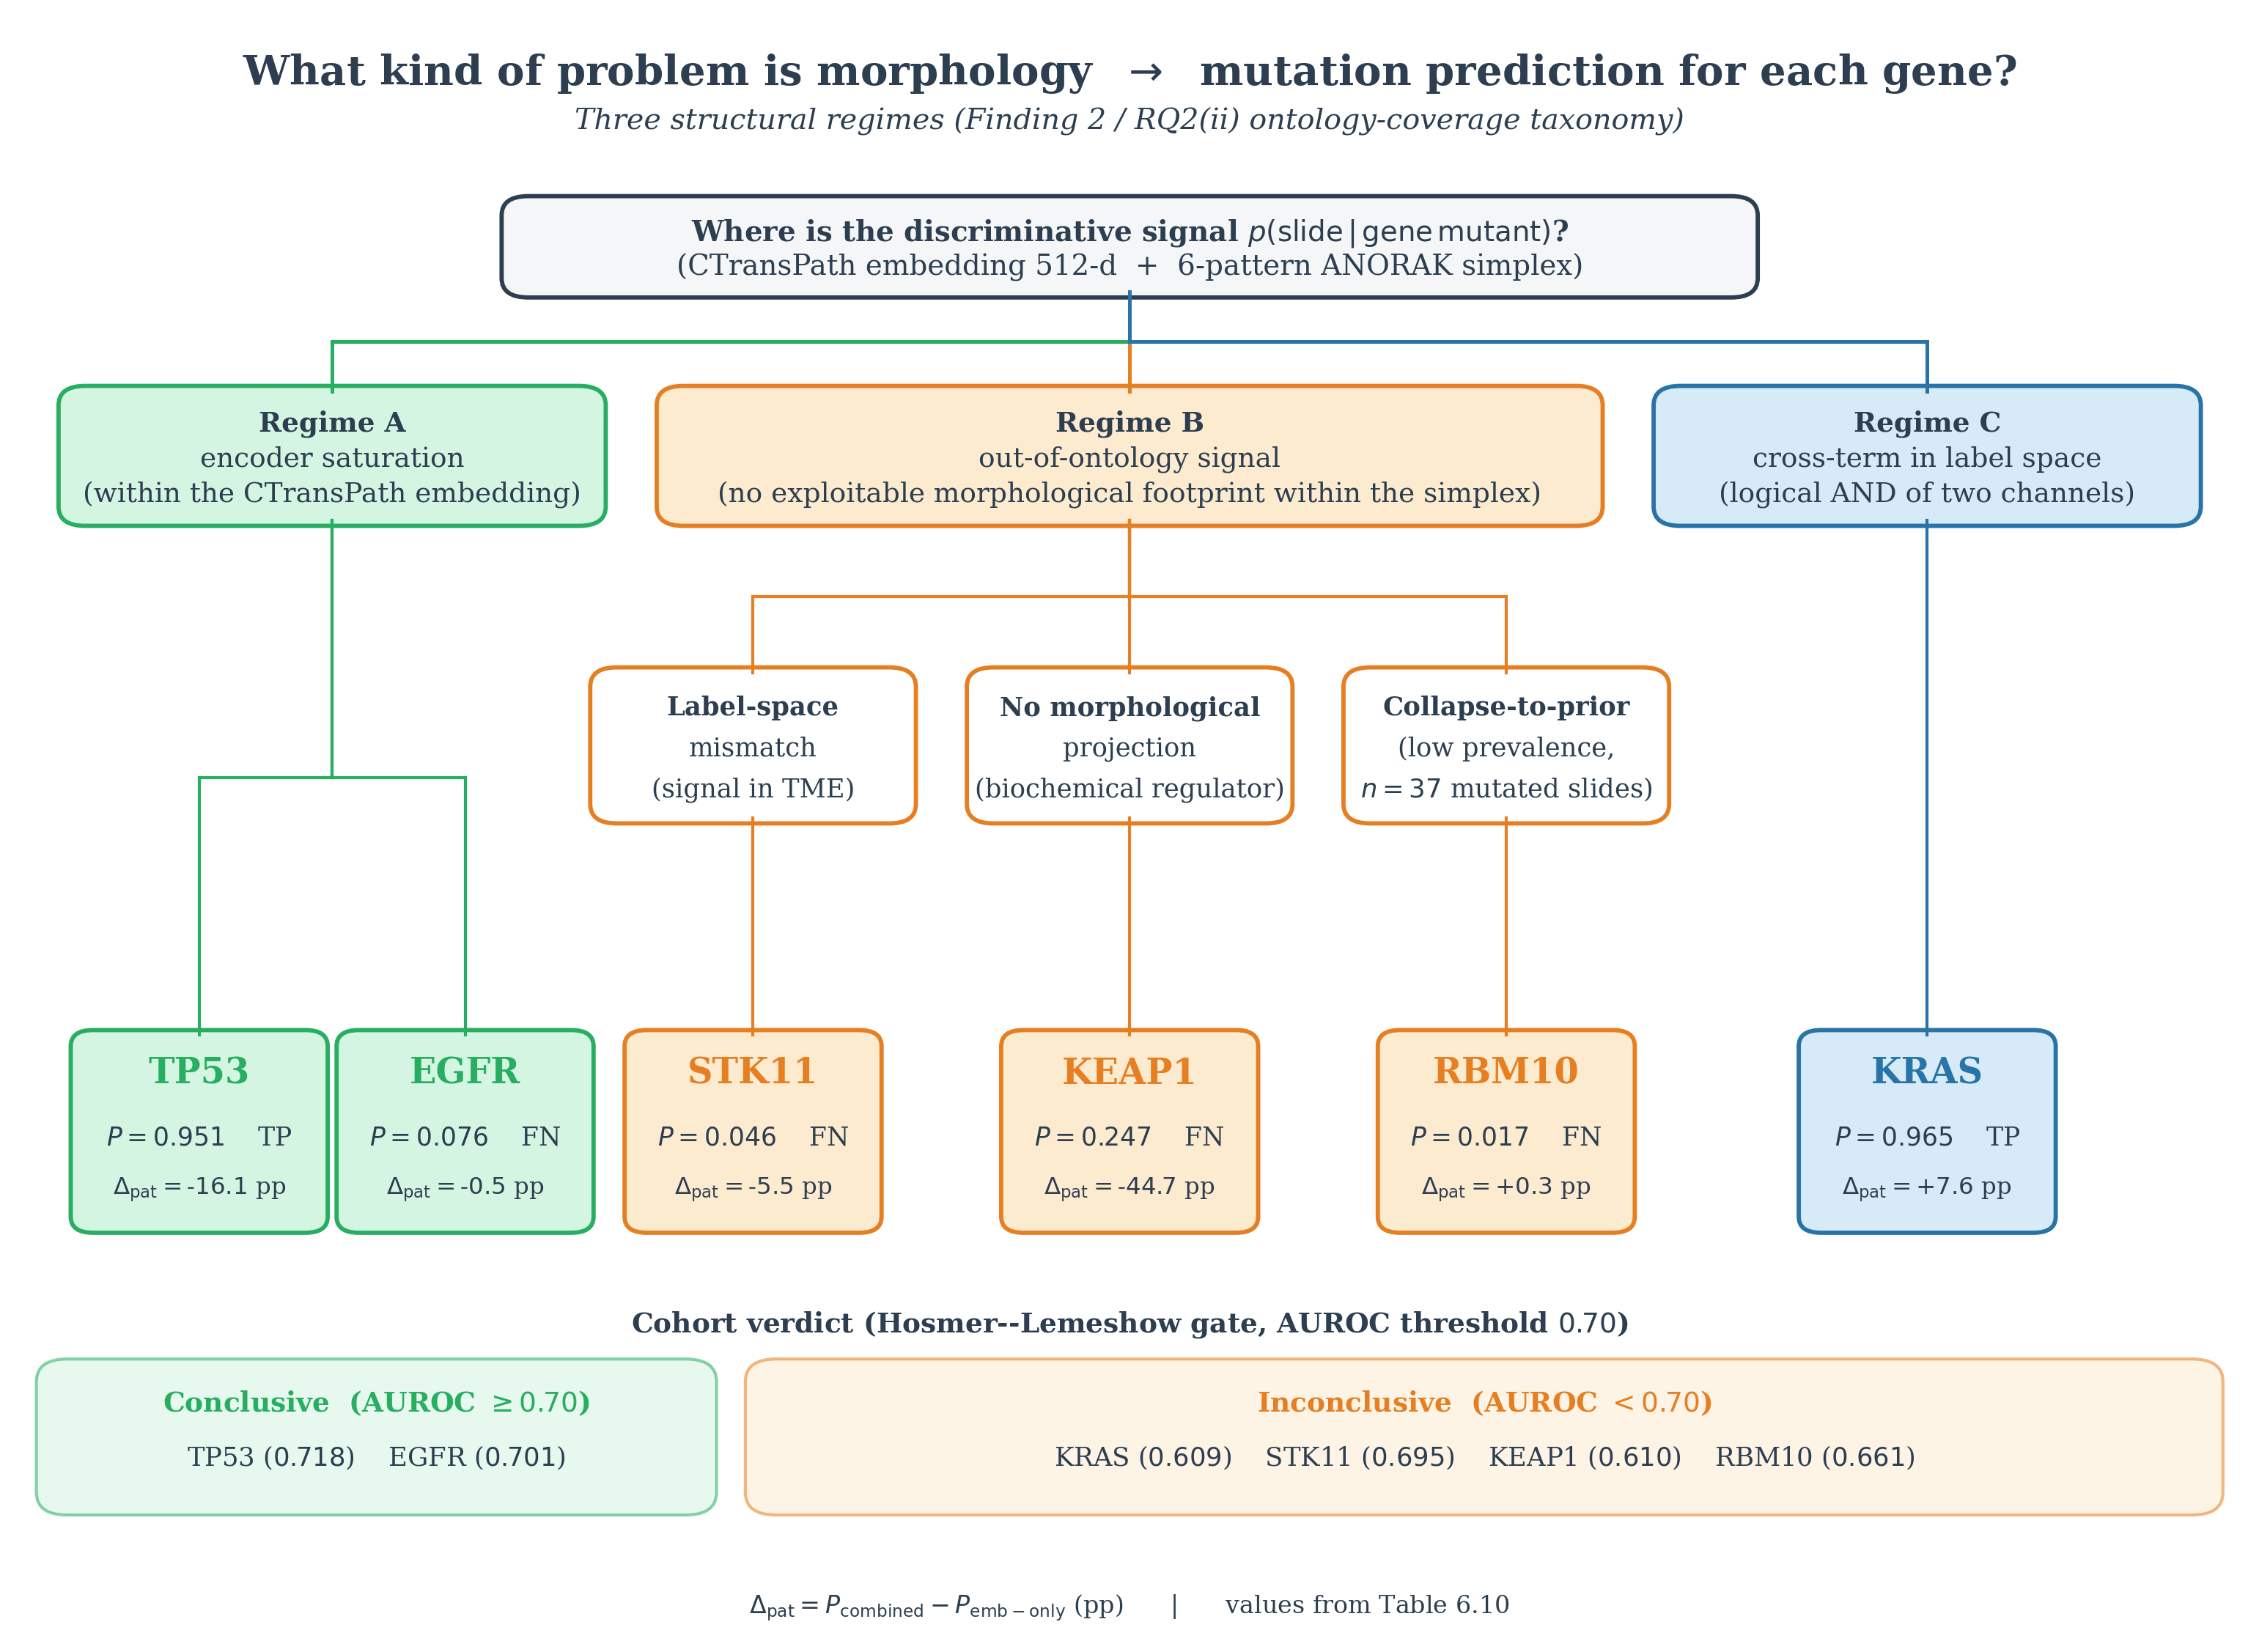
\includegraphics[width=\textwidth]{chapters/figures/signal_tree.png}
\caption[Three structural regimes of morphology--mutation
prediction.]{%
    Decision tree over the six target genes, classified by which
    of the three structural regimes their mutation prediction
    falls under (root question: ``where is the discriminative
    signal $p(\mathrm{slide}\,|\,\mathrm{gene\ mutant})$?'').
    \textbf{Regime~A --- encoder saturation} (left, green):
    the pretrained CTransPath embedding already encodes the
    discriminative signal, so explicit pattern probabilities are
    informationally redundant
    (TP53~\cite{ahn2022tp53highgrade},
    EGFR~\cite{yoshizawa2013egfrmorph}).
    \textbf{Regime~B --- out-of-ontology signal} (centre, orange):
    no representation within the 6-pattern simplex recovers a
    discriminative signal, with three distinct sub-mechanisms
    surfacing in the per-slide ablation
    (Table~\ref{tab:enrichment_summary}):
    \emph{label-space mismatch}, where the signal lives in the
    tumour microenvironment outside the ANORAK schema (STK11);
    \emph{no morphological projection}, an upstream biochemical
    regulator without a robust visible correlate (KEAP1); and
    \emph{collapse-to-prior}, where every channel fails to depart
    from the base rate at low prevalence (RBM10, $n = 37$
    mutated slides; Figure~\ref{fig:rbm10_cleanest_null}).
    \textbf{Regime~C --- cross-term in label space} (right, blue):
    the signal is a logical AND of two existing channels and
    requires a cross-term aggregator (Choquet integral) to be
    read; KRAS reaches $P = 0.965$ via the lepidic--solid
    co-presence that proxies the missing IMA class
    (Figures~\ref{fig:kras_lepidic_solid_proxy},~\ref{fig:kras_mu_subset_lattice}).
    Per-gene cards report the slide-level evidence on the
    representative case ($P$, TP/FN outcome,
    $\Delta_{\mathrm{pat}} = P_{\mathrm{combined}} -
    P_{\mathrm{emb\text{-}only}}$ in pp;
    Table~\ref{tab:enrichment_summary}).
    The bottom band reports the cohort-level Hosmer--Lemeshow
    verdict at the AUROC $0.70$ threshold:
    Regime~A genes (TP53, EGFR) are Conclusive; the four
    Regime~B and~C genes are Inconclusive at population level.
    Note that the slide-level FN at the EGFR card does not
    contradict EGFR's regime~A assignment: the cohort-mean
    AUROC of $0.701$ is Conclusive, but the particular
    representative slide chosen for the case study falls in the
    false-negative tail of the score distribution
    (Section~\ref{sec:eval:tcga:egfr};
    Figure~\ref{fig:egfr_score_overlap}).}
\label{fig:signal_tree}
\end{figure}

\subsection{Finding 3: Soft vs.\ Hard Pattern Encodings Are
Mechanism-Bound, Not Gene-Bound}
\label{sec:eval:mutation:finding3}

Two encodings of the 6-d pattern vector are tested under PI-ABMIL:
the soft fuzzy probability simplex
$\mathbf{p} \in \Delta^5$ produced by the FuzzyArcLoss~V2 classifier,
and a hard one-hot vector $\mathbf{e}_{\arg\max\,\mathbf{p}}$ that
keeps the argmax entry and discards the rest.
The two carry exactly the same information when a single pattern
dominates ($p_k \approx 1$); they diverge when a tile sits between
classes (e.g.\ $p_{k_1} = 0.55$, $p_{k_2} = 0.40$, $p_{k_3} = 0.05$),
where the soft vector preserves the boundary uncertainty as a
feature and the one-hot collapses it to a single argmax.

\begin{table}[ht!]
\centering
\caption{PI-ABMIL (PI, fuzzy) versus Ablation~A (crisp one-hot).
$\Delta = \text{PI} - \text{A}$.}
\label{tab:fuzzy_vs_crisp}
\begin{tabular}{l c c c l}
\hline
\textbf{Gene} & \textbf{PI (fuzzy)} & \textbf{A (crisp)} &
\textbf{$\Delta$} & \textbf{Better} \\
\hline
TP53  & 0.717 & 0.716 & $+$0.001 & Fuzzy \\
EGFR  & 0.694 & 0.695 & $-$0.001 & Crisp \\
STK11 & 0.695 & 0.691 & $+$0.004 & Fuzzy \\
KEAP1 & 0.610 & 0.594 & $+$0.016 & Fuzzy \\
KRAS  & 0.590 & 0.594 & $-$0.004 & Crisp \\
RBM10 & 0.640 & 0.623 & $+$0.017 & Fuzzy \\
\hline
\end{tabular}
\end{table}

\textbf{All six deltas are sub-significant.}
None of the values in Table~\ref{tab:fuzzy_vs_crisp} reaches the
$d \approx 1.2$ MDE bound of a paired test with $K = 5$ folds
(Section~\ref{sec:eval:limitations}).
On its own the table cannot distinguish encoding effects from
fold-variance noise; what it does reveal is that under an additive
head (PI-ABMIL's concatenation) the soft and hard encodings are
mechanically equivalent in expectation: neither carries
information that the head can read.
This is consistent with Finding~1's observation that, across all
six genes, the head---not the encoding---is the bottleneck.

\textbf{The mechanism becomes visible only in regime~C of
Finding~2 (KRAS).}
Within concatenation, fuzzy and crisp tie at $-0.004$
(Table~\ref{tab:fuzzy_vs_crisp}); under FC-MIL's Choquet
aggregator the same fuzzy vector reaches $0.609$---the cohort top
for KRAS (Table~\ref{tab:mutation_luad}).
The soft entropy of the fuzzy encoding is what enables the
Choquet branch to learn the graded interaction
$I_{\,\mathrm{lepidic,\,solid}} = +0.032$
(Section~\ref{sec:eval:mutation:finding2}; full architectural
account in Finding~4); a one-hot vector zeros every cross-term
except the diagonal, structurally preventing the same operator
from finding the same signal.
Soft encodings therefore carry information that an additive head
discards, but only a cross-term consumer extracts it.

\textbf{The KEAP1 and RBM10 cohort lifts are not encoding
evidence.}
The two largest fuzzy-over-crisp deltas in
Table~\ref{tab:fuzzy_vs_crisp}---KEAP1 ($+0.016$) and RBM10
($+0.017$)---should not be read as ``boundary uncertainty carries
diagnostic information for these genes''.
Regime~B of Finding~2 already established that no representation
within the 6-pattern simplex recovers signal for KEAP1 (no
morphological projection) or RBM10 (collapse-to-prior at low
prevalence).
The deltas are most economically read as a small regularising
effect of the soft entropy on the low-attention bulk of the cohort
plus fold-variance on a 37-slide minority class
(RBM10 fold std $0.05$--$0.10$; Section~\ref{sec:eval:limitations}).

\textbf{Take-away.}
The original analytical contribution is therefore
\emph{mechanism-bound rather than gene-list-bound}: the soft-vs-hard
distinction matters when, and only when, the consumer head can
read joint activations across channels.
Within additive concatenation the two encodings are
interchangeable up to fold variance regardless of which structural
regime the gene sits in.

\subsection{Finding 4: The Pattern Stream Alone Tests Label-Space
Coverage Directly}
\label{sec:eval:mutation:finding4}

Condition B3 is the same ABMIL backbone as B2 trained on the 6-d
pattern probability vector with the 512-d embedding removed.
It answers the most direct question one can ask of the white-box
channel: \emph{does the 6-pattern simplex carry
mutation-discriminative signal at all, on its own?}
B3's per-gene AUROCs span $0.545$--$0.653$ (5-fold CV;
Table~\ref{tab:mutation_luad}), systematically below B2
($0.597$--$0.718$).
The pattern channel is not a substitute for the visual embedding
on any gene.
Two anomalies relative to the default ``B2~$>$~B3~$>$~B1'' ordering
reveal mechanism rather than noise.

\paragraph{KRAS --- the cross-term route, formalised.}
B3 collapses to $0.545$ on KRAS (essentially chance), the most
striking result in Table~\ref{tab:mutation_luad}.
Figure~\ref{fig:kras_two_routes} traces why through the two routes
the pattern stream offers from the 6-d input to the classifier.

\emph{Route~1 (a dedicated channel) is structurally closed.}
ANORAK has no IMA / mucinous channel
(Section~\ref{sec:uc:luad_histology}; centre panel of
Figure~\ref{fig:kras_lepidic_solid_proxy}).

\emph{Route~2 (a logical AND of two channels) is closed for any
additive head.}
The IMA architecture can be encoded as the joint activation of
\emph{lepidic} and \emph{solid} on the same slide
(Section~\ref{sec:eval:mutation:finding2}).
A linear-concatenation head cannot represent this AND
($w_l p_l + w_s p_s \neq p_l \cdot p_s$).
The numbers confirm the regime: B3 collapses to $0.545$, and
PI-ABMIL---which puts the embedding back alongside the pattern
vector but keeps the additive head---still reaches only $0.590$,
below B2's $0.607$ (Table~\ref{tab:mutation_luad}, KRAS column).
Within an additive head the soft-vs-hard delta is only $-0.004$
(Table~\ref{tab:fuzzy_vs_crisp}): the bottleneck is the head, not
the encoding (Finding~3).

\emph{Route~2 opens under Choquet aggregation.}
FC-MIL replaces the additive head with a Choquet integral that
has 15 trainable pairwise interaction indices $I_{kl}$, each
firing only when both $p_k$ and $p_l$ are jointly high.
The trained model learns $I_{\,\mathrm{lepidic,\,solid}} = +0.032$
(Table~\ref{tab:choquet_interactions}) and recovers KRAS to
$0.609$, above B2 (bottom strip of
Figure~\ref{fig:kras_two_routes}).
The KRAS signal is therefore present in the embedding (B2 reaches
$0.607$); the only architecture that can read it through the
pattern stream is one with a cross-term head.
The full per-gene Choquet behaviour is mapped in Finding~6
(Section~\ref{sec:eval:mutation:finding6};
Figure~\ref{fig:choquet_regimes}).

\begin{figure}[ht!]
  \centering
  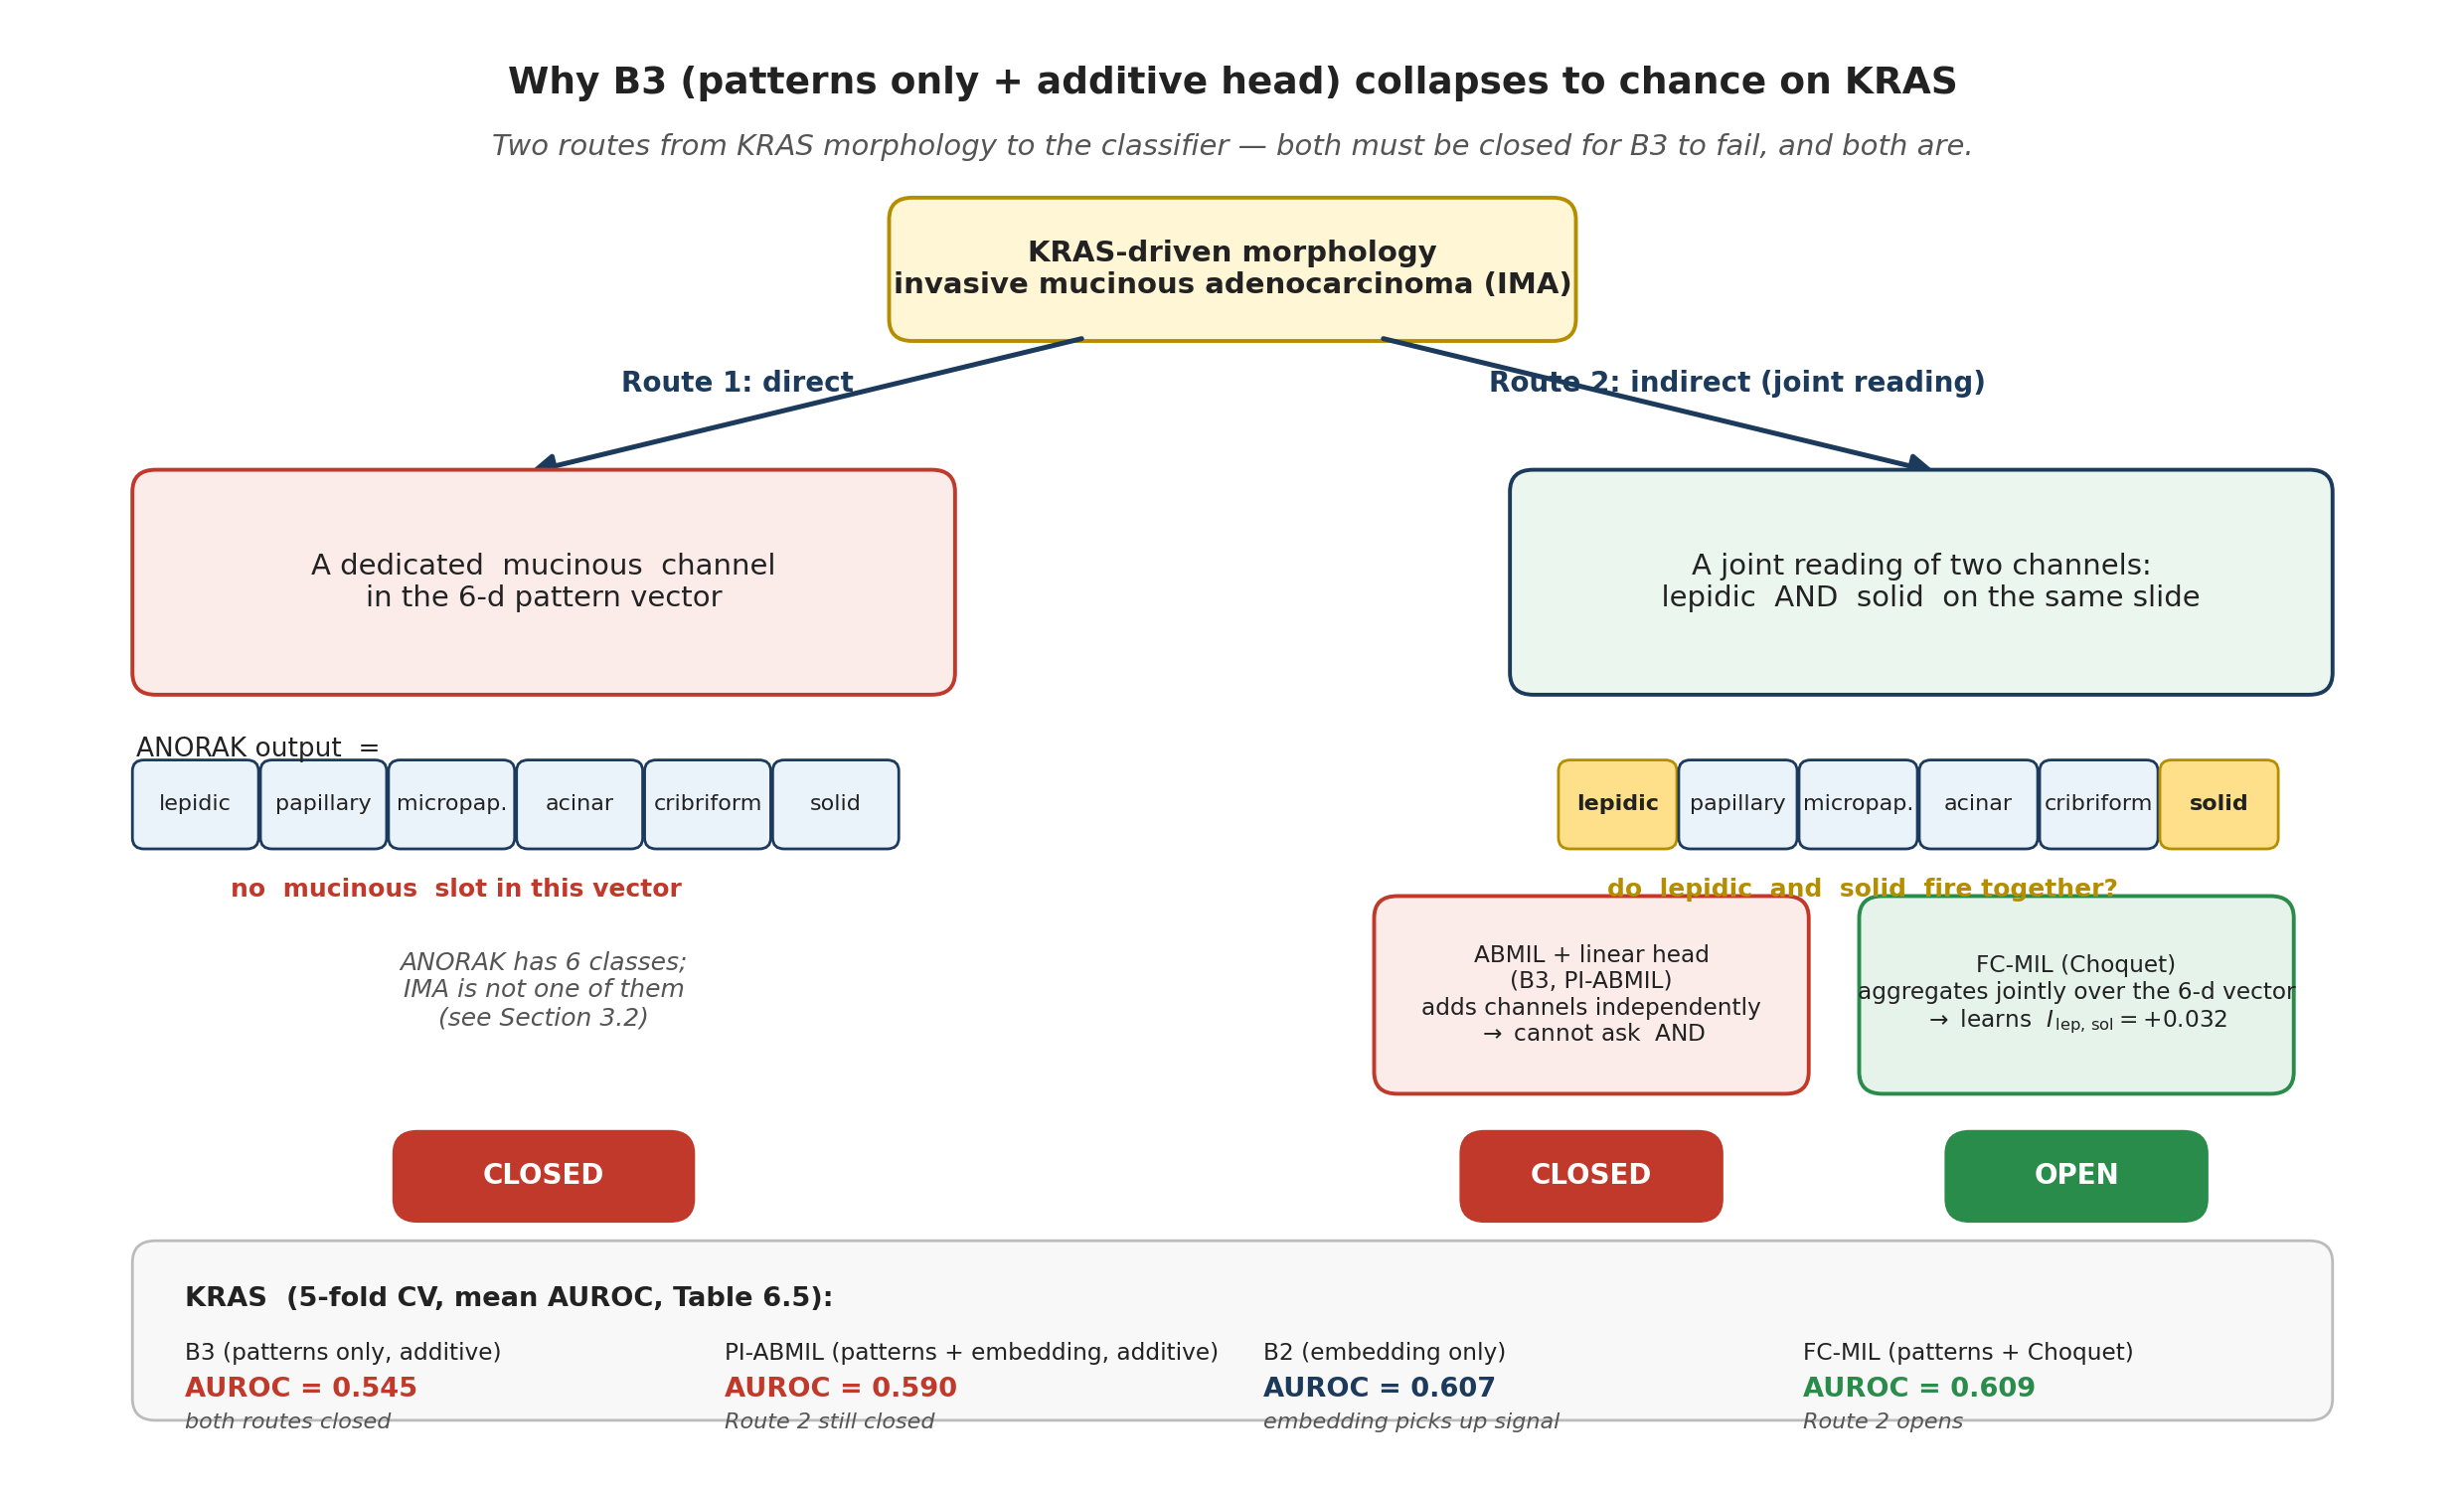
\includegraphics[width=\textwidth]{chapters/figures/kras_two_routes.png}
  \caption[Why B3 collapses to chance on KRAS: two routes, both
    closed]{%
    Two routes from a KRAS signal to the classifier through a 6-d
    pattern vector.
    Route~1 fails because ANORAK has no mucinous channel
    (Section~\ref{sec:uc:luad_histology}).
    Route~2 fails for additive heads (B3, PI-ABMIL) but opens for
    FC-MIL's Choquet aggregator, which encodes the joint reading as
    $I_{\,\mathrm{lepidic,\,solid}} = +0.032$
    (Table~\ref{tab:choquet_interactions}).
    Bottom strip: KRAS mean AUROC over 5-fold CV
    (Table~\ref{tab:mutation_luad}).}
  \label{fig:kras_two_routes}
\end{figure}

\paragraph{Two B3 anomalies, one regime each.}

\emph{RBM10 --- low-prevalence regulariser regime}
(Figure~\ref{fig:b3_regimes}, left).
B3 ($0.653$) is the only condition in the table where the
pattern-only stream beats the embedding-only baseline
(B2~$= 0.642$; Table~\ref{tab:mutation_luad}, RBM10 column).
RBM10 is the lowest-prevalence gene at 5.4\% (37 mutated slides;
Section~\ref{sec:uc:tcga:genes}); at that scarcity B3's 6-d input
is roughly $85\times$ smaller than B2's 512-d input and acts as
an implicit regulariser on a head that B2 over-parameterises.
This is consistent with RBM10's collapse-to-prior diagnosis from
Finding~2 (regime~B): B3 wins by \emph{not} having room to
overfit, not by having found discriminative signal in the pattern
simplex.

\emph{EGFR --- concentrated-signal regime}
(Figure~\ref{fig:b3_regimes}, centre).
For EGFR the slide-level pattern composition---particularly the
lepidic-predominant architecture documented as EGFR-enriched in
the
literature~\cite{suda2017egfrlepidic,yoshizawa2011iaslcpattern}---carries
most of the pattern-channel discriminative bits.
B1 (XGBoost on slide-level pattern frequencies, no attention)
therefore ties B3 (B1~$= 0.634 \approx$~B3~$= 0.625$,
Table~\ref{tab:mutation_luad}), even though B1 has no access to
the within-slide attention structure that ABMIL exploits.
B2~$= 0.701$ still wins on the embedding, consistent with EGFR's
Regime~A diagnosis from Finding~2: CTransPath captures the lepidic
signature \emph{plus} finer cellular features (nuclear shape,
glandular cytology) that the 6-channel pattern simplex does not
expose.
The B1$\,\approx\,$B3 tie is therefore an observation \emph{about
the internal structure of the pattern stream} (slide-level
averaging is as good as tile-level attention \emph{within} the
6-channel simplex), not a competitor to B2; the embedding stream
remains the dominant pathway.
This is the only gene in the cohort where a pattern-frequency
classifier captures most of what attention-weighted aggregation
\emph{over the pattern channel} captures, and Finding~5 reads it
alongside the rest of the XGBoost benchmark.

\emph{Default regime --- TP53, STK11, KEAP1, KRAS}
(Figure~\ref{fig:b3_regimes}, right).
On the remaining four genes neither anomaly applies and the
canonical ordering B2~$>$~B3~$>$~B1 holds
(Table~\ref{tab:mutation_luad}).
B3~$>$~B1 on five of six genes also without the embedding stream,
confirming that attention-weighted tile-level aggregation recovers
more information than slide-level averaging.

\begin{figure}[ht!]
  \centering
  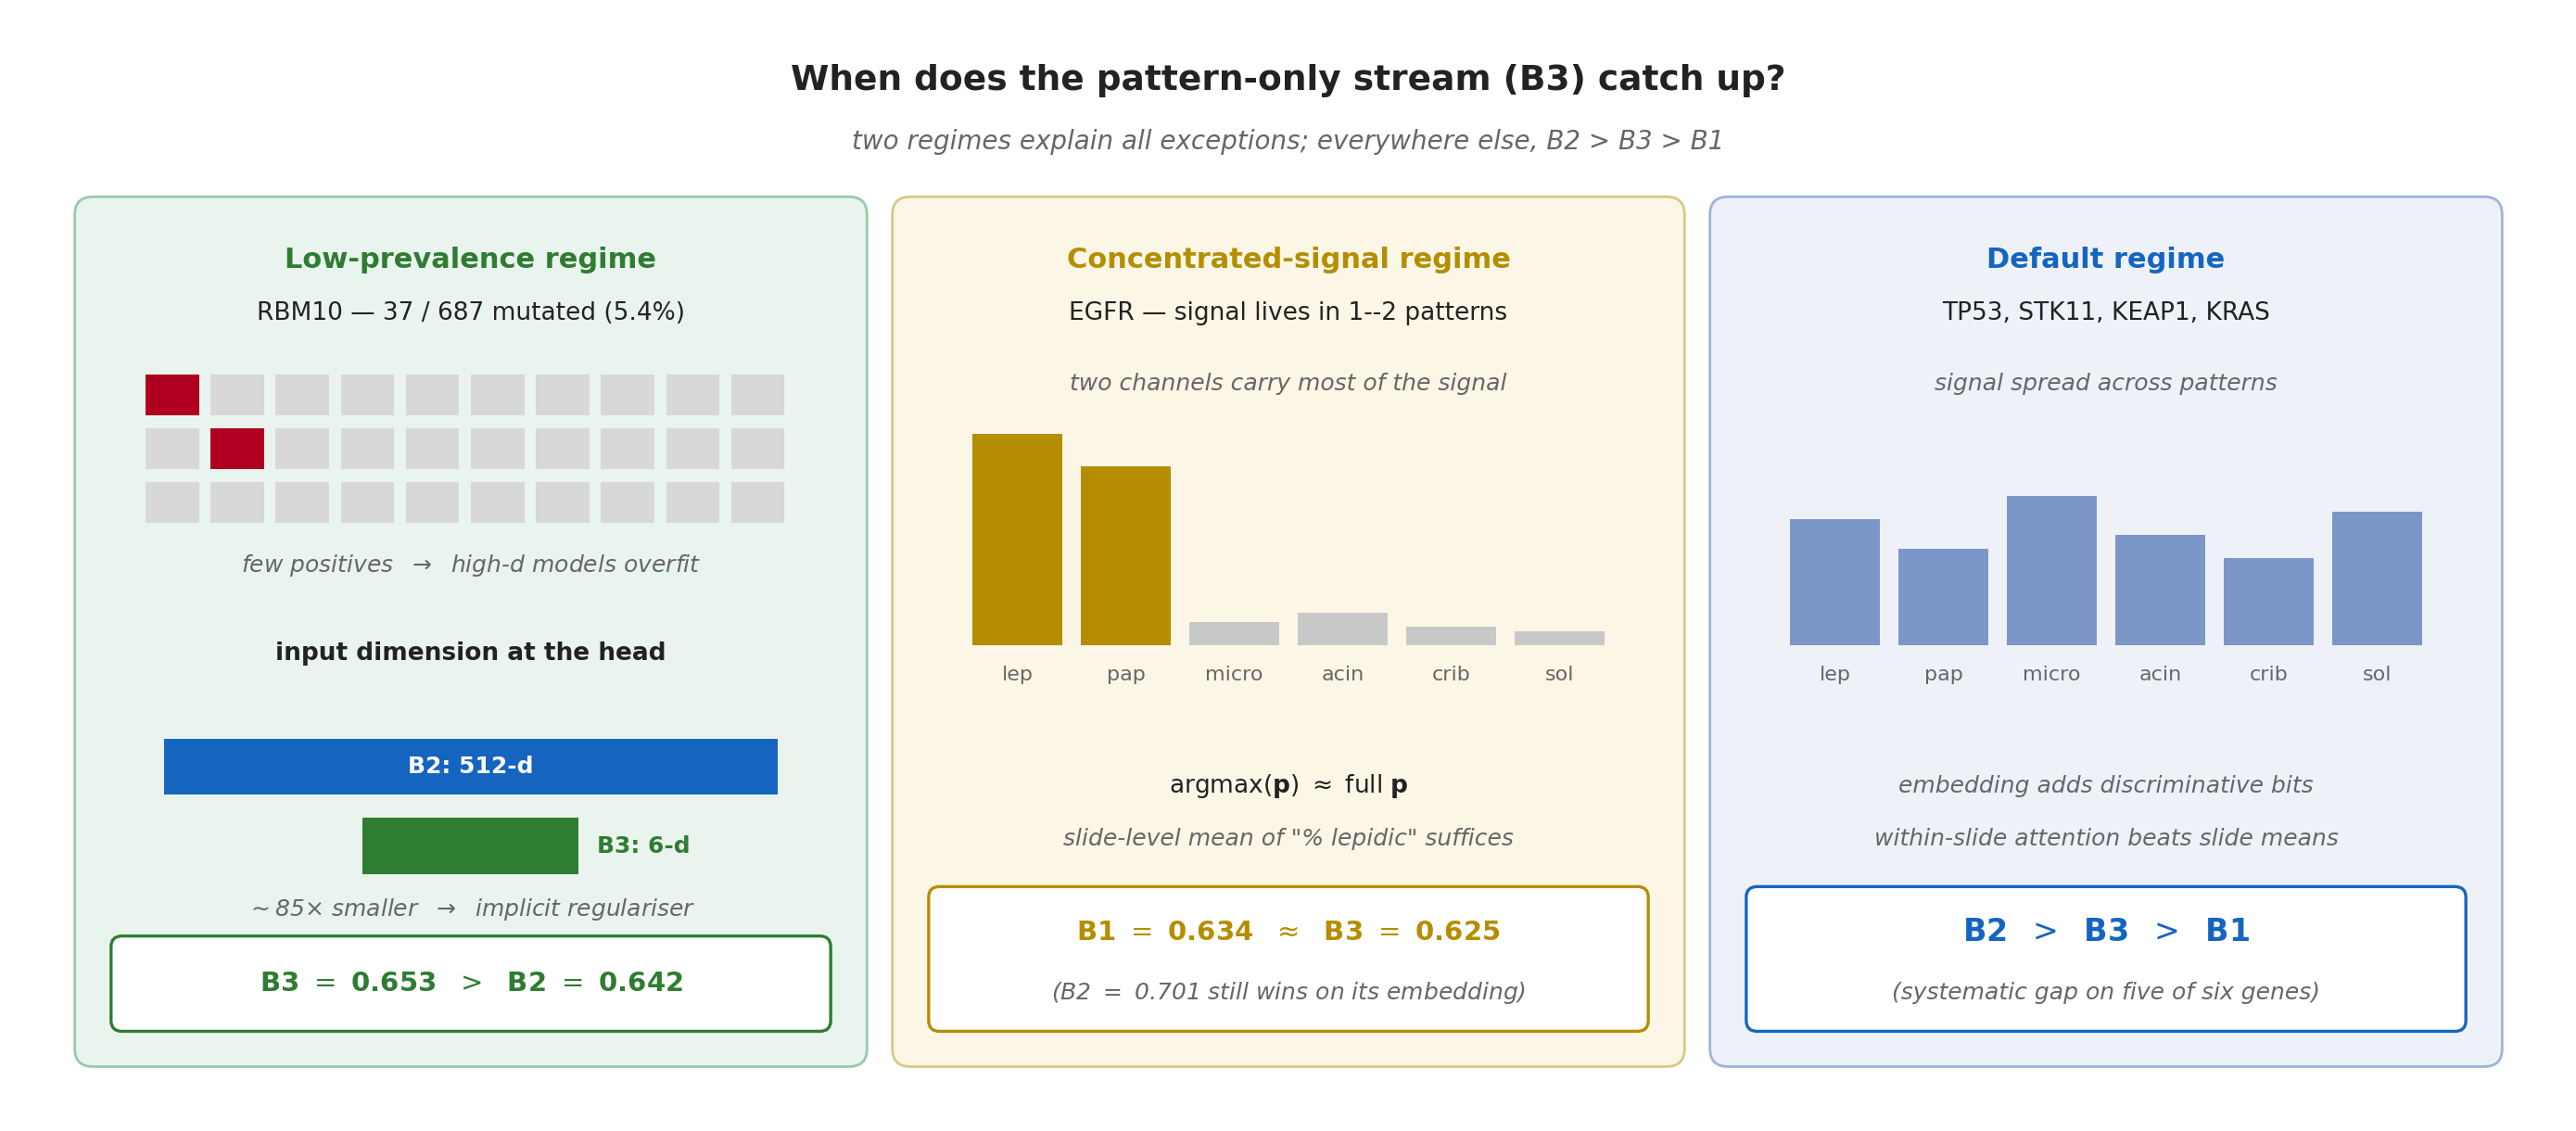
\includegraphics[width=\textwidth]{chapters/figures/b3_regimes.png}
  \caption[When does the pattern-only stream (B3) catch up?]{%
    Two regimes explain every B3 anomaly in
    Table~\ref{tab:mutation_luad}.
    \emph{Left}: in the low-prevalence regime (RBM10, 5.4\%), B3's
    6-d input acts as an implicit regulariser against B2's 512-d
    embedding ($\sim$$85\times$ smaller), and B3 outperforms B2.
    \emph{Centre}: in the concentrated-signal regime (EGFR, signal in
    1--2 patterns), the argmax of the 6-d vector and the slide-level
    mean of ``\% lepidic'' both carry most of the signal, so B1 ties
    B3.
    \emph{Right}: when neither regime applies (TP53, STK11, KEAP1,
    KRAS), the canonical hierarchy B2~$>$~B3~$>$~B1 is recovered.}
  \label{fig:b3_regimes}
\end{figure}

\subsection{Finding 5: XGBoost on Pattern Frequencies Confirms the
Structural Taxonomy from a Different Angle}
\label{sec:eval:mutation:finding5}

B1 is the simplest possible white-box predictor for this task: an
XGBoost classifier on the 6-d slide-level mean of pattern
frequencies, with no within-slide attention, no fuzzy entropy, and
no embedding channel.
It asks \emph{``how much can a non-attention non-deep classifier
do with only the average pattern composition of a slide?''}---a
direct measurement of the discriminative content of the simplex
under maximal feature simplification.

Per-gene B1 AUROCs span $0.474$--$0.634$ with cohort mean $0.530$
(Table~\ref{tab:mutation_luad}; Figure~\ref{fig:b1_per_gene}),
between random ($0.500$) and B3 ($0.607$), well below B2 ($0.658$).
Three observations align directly with the structural taxonomy of
Finding~2:

\paragraph{Top --- EGFR ($0.634$).}
The single-gene exception is consistent with the
concentrated-signal regime introduced as the EGFR anomaly in
Finding~4 (Figure~\ref{fig:b3_regimes}, centre):
EGFR mutations are associated with lepidic-predominant
morphology accompanied by papillary
growth~\cite{yoshizawa2013egfrmorph}, so the signal lives in only
1--2 of the six pattern channels and the slide-level mean of those
channels captures most of the discriminative bits even without
attention.
For the deployment-side reading this means a lightweight XGBoost
classifier is a viable practical approximation when deep-learning
infrastructure is not available---but \emph{only} for genes whose
signal is concentrated in 1--2 patterns.

\paragraph{Bottom --- RBM10 ($0.474$) and KEAP1 ($0.489$), both
below random.}
These two below-chance results are not B1 failure modes; they are
B1 \emph{success at measuring the absence of signal in the
simplex} for these genes, from a different angle than the
per-slide ablation already used in Finding~2 (regime~B): if a
calibrated XGBoost on slide-level pattern frequencies cannot reach
random, then any architecture downstream of the same pattern
features is unlikely to find what is not there.
The result is consistent with the no-morphological-projection
diagnosis for KEAP1 and the collapse-to-prior diagnosis for RBM10,
and it is reproduced by the Choquet branch behaviour in
Finding~6 from yet a third angle (engaged-but-unproductive
regime).

\paragraph{Mean.}
The cohort mean of $0.530$ (Figure~\ref{fig:b1_per_gene}, dashed)
is well above random but well below B2: B1 is non-trivial for the
four other genes (in the regime where signal is spread across
patterns and within-slide attention matters), yet the
attention-weighted aggregation that B3 and B2 perform extracts
substantially more discriminative information than slide-level
averaging when the signal is not concentrated.

\begin{figure}[ht!]
  \centering
  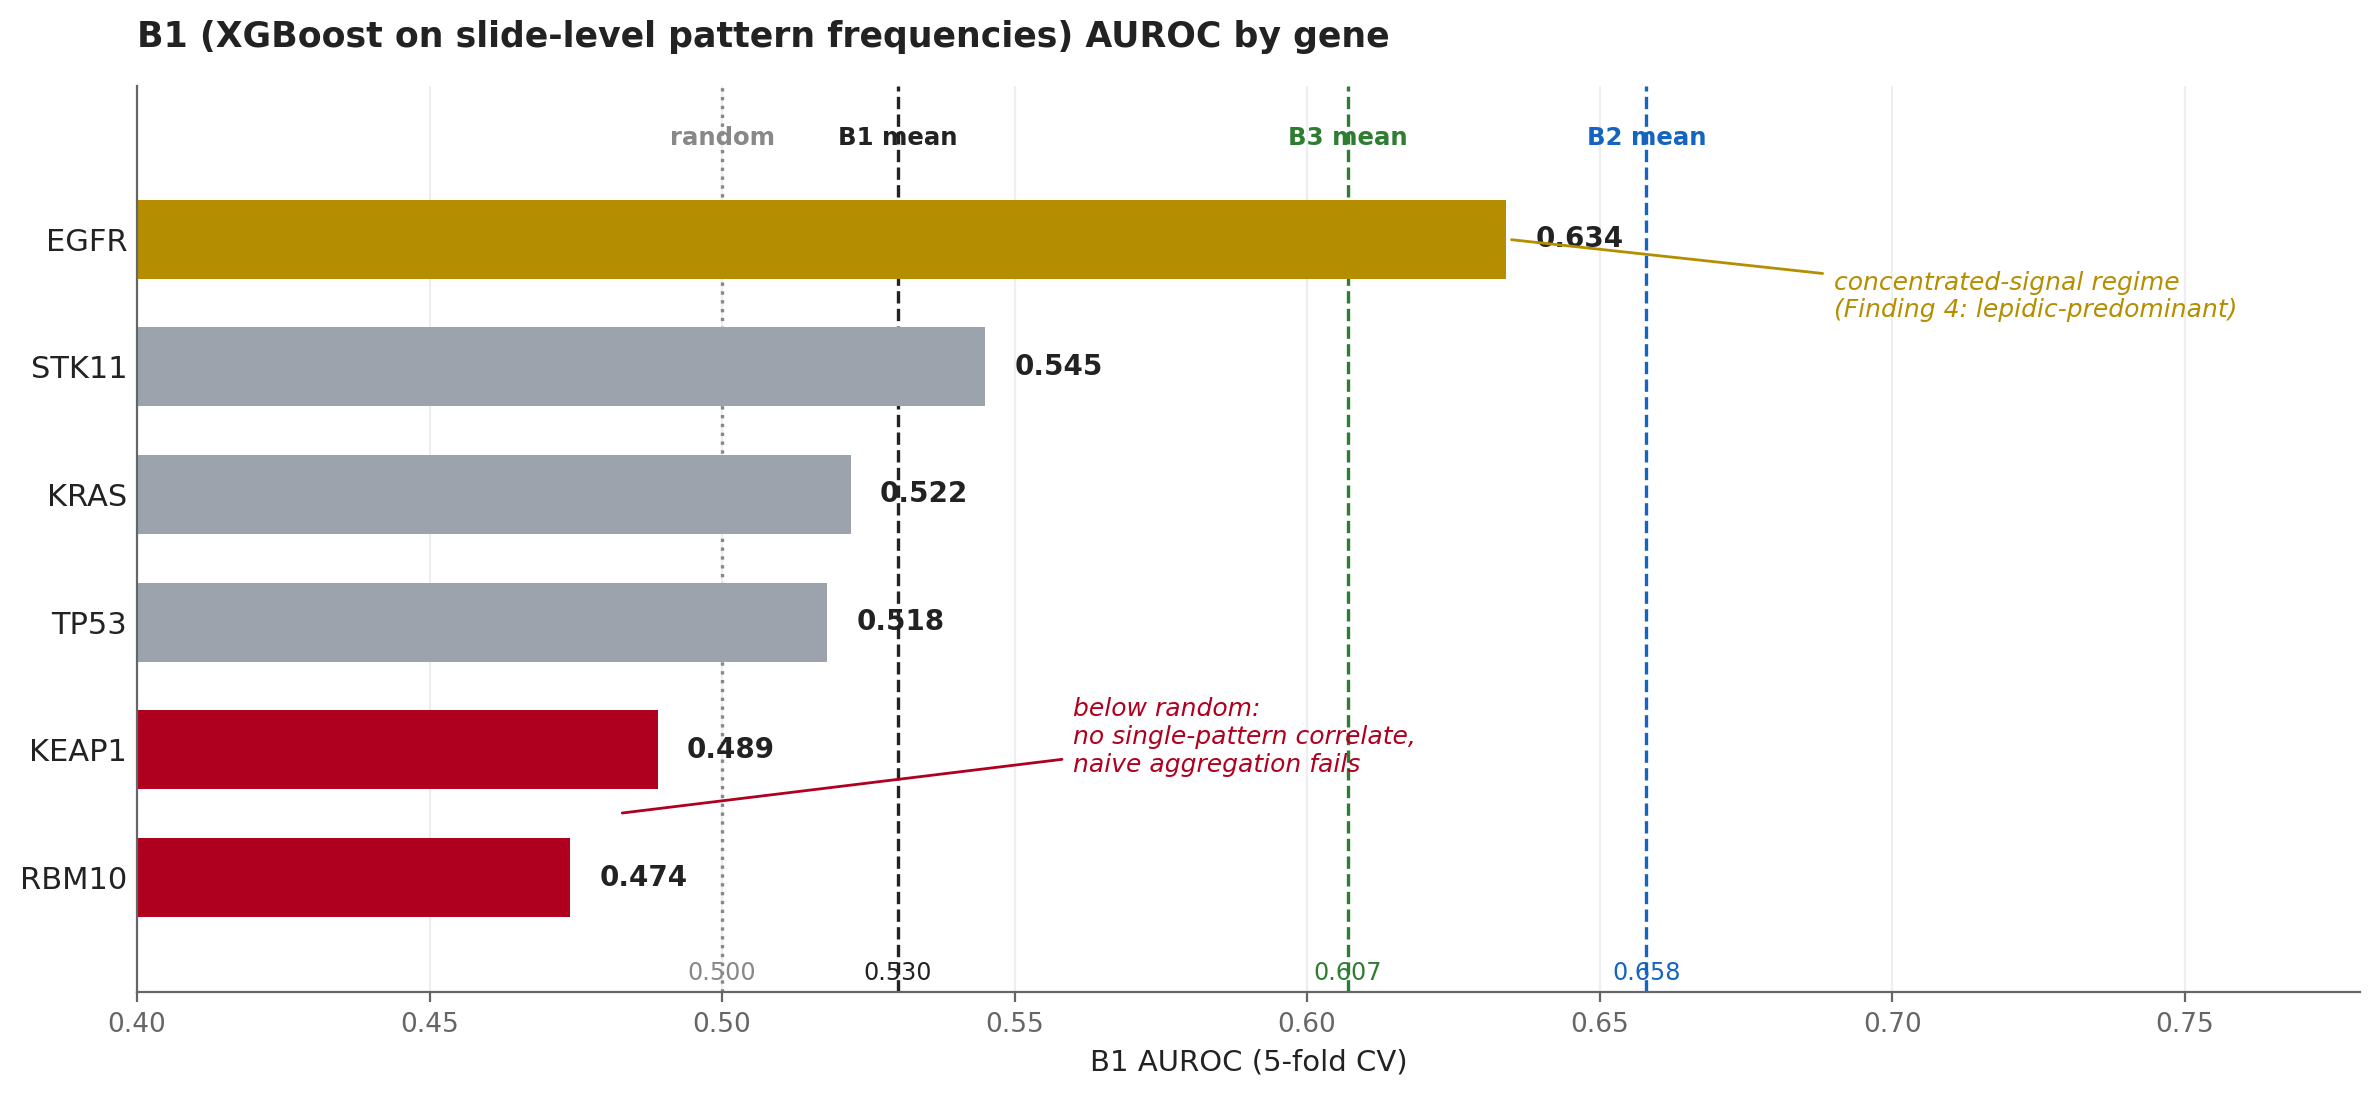
\includegraphics[width=\textwidth]{chapters/figures/b1_per_gene.png}
  \caption[B1 (XGBoost on slide-level pattern frequencies) AUROC by
    gene]{%
    B1 AUROC by gene (5-fold CV; values from
    Table~\ref{tab:mutation_luad}).
    EGFR ($0.634$, amber) sits at the top via the concentrated-signal
    regime of Finding~4 (Figure~\ref{fig:b3_regimes}, centre);
    KEAP1 ($0.489$) and RBM10 ($0.474$, red) fall below the random
    line, indicating that slide-level pattern frequencies carry no
    usable signal for these labels.
    Reference lines mark random ($0.500$), the B1 mean ($0.530$), the
    B3 mean ($0.607$), and the B2 mean ($0.658$).}
  \label{fig:b1_per_gene}
\end{figure}

\subsection{Finding 6: Choquet Branch Behaviour Confirms the
Structural Taxonomy}
\label{sec:eval:mutation:finding6}

FC-MIL is the dual-pathway architecture: the same ABMIL encoder as
B2 (operating on the 512-d CTransPath embedding), plus a parallel
Choquet integral branch on the 6-d pattern probabilities with a
21-parameter 2-additive fuzzy measure (6 singleton Shapley values
$\phi_k$, 15 pairwise interaction indices $I_{kl}$).
Total trainable parameters $\sim 266\,000$.
The comparison FC-MIL vs.\ B2 isolates the contribution of the
Choquet branch on top of the shared ABMIL encoder.
At the cohort mean FC-MIL ($0.653$) is non-inferior to B2 ($0.658$)
within fold variance ($\Delta = -0.005$, below the $d \approx 1.2$
MDE bound; Section~\ref{sec:eval:limitations}); the per-gene
behaviour, however, splits into three regimes that map directly
onto the structural taxonomy of Finding~2.

\paragraph{Constructive --- KRAS only (regime~C of Finding~2).}
The branch locks onto a stable cross-term:
$I_{\,\mathrm{lepidic,\,solid}} = +0.032$, the largest of the 15
pairs (Table~\ref{tab:choquet_interactions}), with a secondary
$I_{\,\mathrm{solid,\,acinar}} = +0.025$.
The lepidic$\times$solid pair is the IMA proxy mechanism formalised
in Findings~2 and~4, and the variance map confirms that it is
\emph{stable} across folds: KRAS sits in the
\emph{productive\,+\,stable} quadrant of
Figure~\ref{fig:choquet_variance_map}
($\Delta\mathrm{AUROC} = +0.002$, $\Delta\sigma = -0.019$).
This is the only gene in the cohort where the Choquet branch
provides a non-trivial discriminative contribution beyond the
shared embedding pathway.
Per-slide effect: the global $I$ values modulate
$P(\mathrm{mut})$ on each slide by an amount that depends on that
slide's actual lepidic and solid memberships, so the
$+3.2$\,pp magnitude does not translate to a uniform per-slide
uplift.

\paragraph{Silent --- TP53, EGFR (regime~A of Finding~2).}
The branch trains to a near-uniform fuzzy measure
($\phi_k \approx 1/6$ for all $k$, $|I_{kl}| \ll 0.1$), so the
Choquet integral reduces to an additive weighted average and
contributes no extra discriminative structure.
The shared embedding pathway already saturates the morphological
signal (Finding~2, regime~A); $|\Delta\mathrm{AUROC}| \leq 0.005$
between FC-MIL and B2 with $\Delta\sigma < 0$
(Figure~\ref{fig:choquet_variance_map}, lower-left quadrant: ``not
engaged'').
The branch is inert by saturation: no engagement, no harm.
Its value is interpretive---the Shapley values and interaction
indices remain readable as evidence that no pattern-level
preference is needed for these two genes.

\paragraph{Engaged but unproductive --- STK11, KEAP1, RBM10
(regime~B of Finding~2).}
The branch trains over a feature space that carries no
discriminative signal (the three out-of-ontology sub-mechanisms
of regime~B), and exhibits three different forms of unproductive
exploration:
\begin{itemize}
  \item \emph{KEAP1 (spread).}
  KEAP1's no-morphological-projection diagnosis manifests as
  probability mass diffused across all six patterns rather than
  concentrated in any pair, and the Choquet integral's
  multiplicative inductive bias is therefore the wrong fit:
  FC-MIL ($0.589$) is outperformed by both B2 ($0.597$) and
  PI-ABMIL ($0.610$;~Table~\ref{tab:mutation_luad}).
  KEAP1 sits near the origin of
  Figure~\ref{fig:choquet_variance_map}
  ($\Delta\mathrm{AUROC} \approx -0.008$, $\Delta\sigma \approx 0$):
  marginal mean degradation, no fold-specific noise.
  \item \emph{STK11 (engaged but never converges).}
  The branch engages fold-specifically (high
  $\Delta\sigma = +0.035$;
  Figure~\ref{fig:choquet_variance_map}, upper-left
  ``engagement without conversion'') without ever locking onto a
  discriminative pair.
  This is the label-space mismatch of Finding~2 visible at the
  parameter level: each fold's training set offers a different
  spurious correlate, the optimiser explores them, none generalises.
  Net AUROC effect: $\Delta\mathrm{AUROC} = -0.026$.
  \item \emph{RBM10 (architectural negative control).}
  On the seed-42 trained model the singleton spread is $0.0007$
  with all $|I_{kl}| < 0.01$
  (Section~\ref{sec:eval:interp:choquet}), so the branch is
  effectively empty.
  Across folds the branch explores fold-specifically without
  locking onto any pair (RBM10 sits in the
  \emph{productive + exploratory} quadrant of
  Figure~\ref{fig:choquet_variance_map},
  $\Delta\mathrm{AUROC} = +0.019$, $\Delta\sigma = +0.009$); the
  exploration is unstable, and the seed-42 model converges to
  near-zero parameters.
  The cohort-mean lift over B2 originates entirely in the shared
  embedding pathway: at 5.4\% prevalence the dual-pathway training
  regime perturbs the embedding loss in a way that, on this
  low-prevalence gene, happens to produce a slight improvement,
  but the Choquet branch carries no signal.
  Equivalently, FC-MIL on RBM10 behaves like an ensemble whose
  second branch is silent---the lift comes from the active branch,
  not from the silent one finding new signal.
\end{itemize}

\paragraph{Why the variance map matters.}
A mean-AUROC view alone (Figure~\ref{fig:choquet_regimes}) cannot
distinguish ``the branch is silent because the embedding saturates''
(TP53, EGFR) from ``the branch engages but cannot find signal in
the simplex'' (STK11, KEAP1, RBM10): both can give
$|\Delta\mathrm{AUROC}| \approx 0$ against B2.
The variance axis of Figure~\ref{fig:choquet_variance_map}
($\Delta\sigma$) makes the difference observable: silent branches
\emph{lower} fold variance (the trained measure converges to a
single near-uniform fixed point), engaged-but-unproductive branches
\emph{raise} it (each fold's optimiser explores a different
unstable subset).
The two diagnostics together separate regime~A from regime~B at the
parameter level, and confirm that the only gene where the Choquet
branch operates as an active discriminative module is KRAS
(regime~C).

\begin{figure}[H]
  \centering
  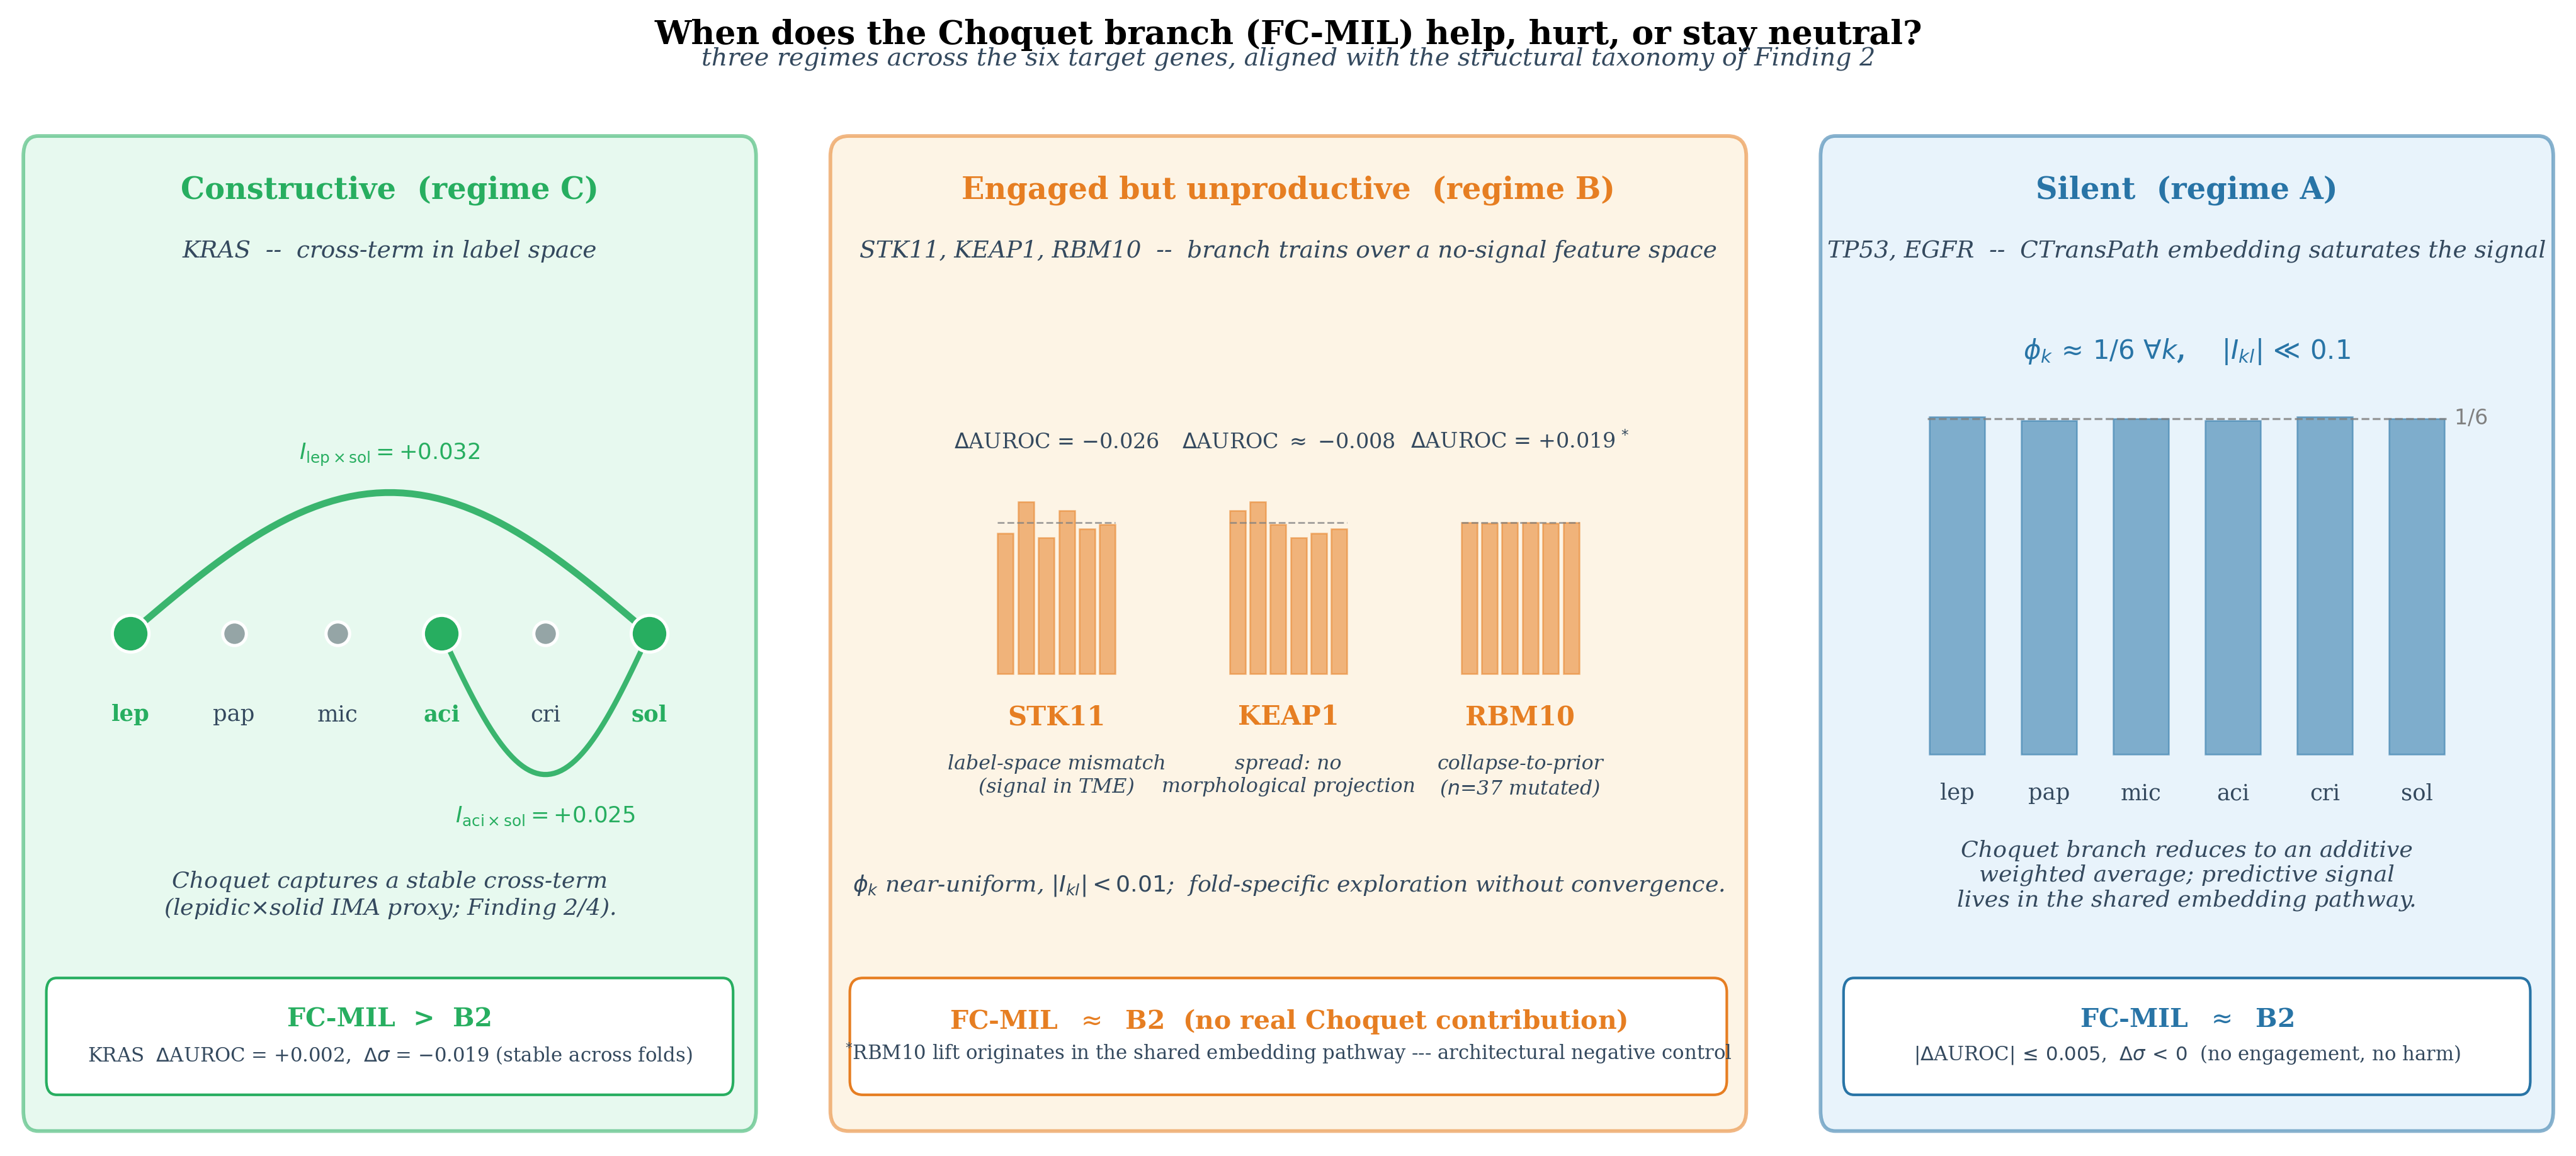
\includegraphics[width=\textwidth]{chapters/figures/choquet_regimes.png}
  \caption[When does the Choquet branch help, hurt, or stay
    neutral?]{%
    Three regimes characterise FC-MIL across the six target genes,
    aligned with the structural taxonomy of Finding~2.
    \emph{Left}: constructive (KRAS, regime~C) --- the Choquet
    branch captures the lepidic$\times$solid IMA proxy
    ($I = +0.032$; Table~\ref{tab:choquet_interactions}) and FC-MIL
    beats B2.
    \emph{Centre}: engaged-but-unproductive sub-case ``spread''
    (KEAP1, regime~B/no-morphological-projection) --- probability
    mass diffused across all six patterns, no pair to capture,
    FC-MIL underperforms both B2 and PI-ABMIL.
    \emph{Right}: silent + engaged-but-unproductive sub-cases
    (TP53/EGFR in regime~A; STK11/RBM10 in regime~B) ---
    near-uniform Shapley values and small $|I_{kl}|$;
    indistinguishable on the AUROC axis but separable on the
    variance axis (Figure~\ref{fig:choquet_variance_map}).}
  \label{fig:choquet_regimes}
\end{figure}

\begin{figure}[ht!]
  \centering
  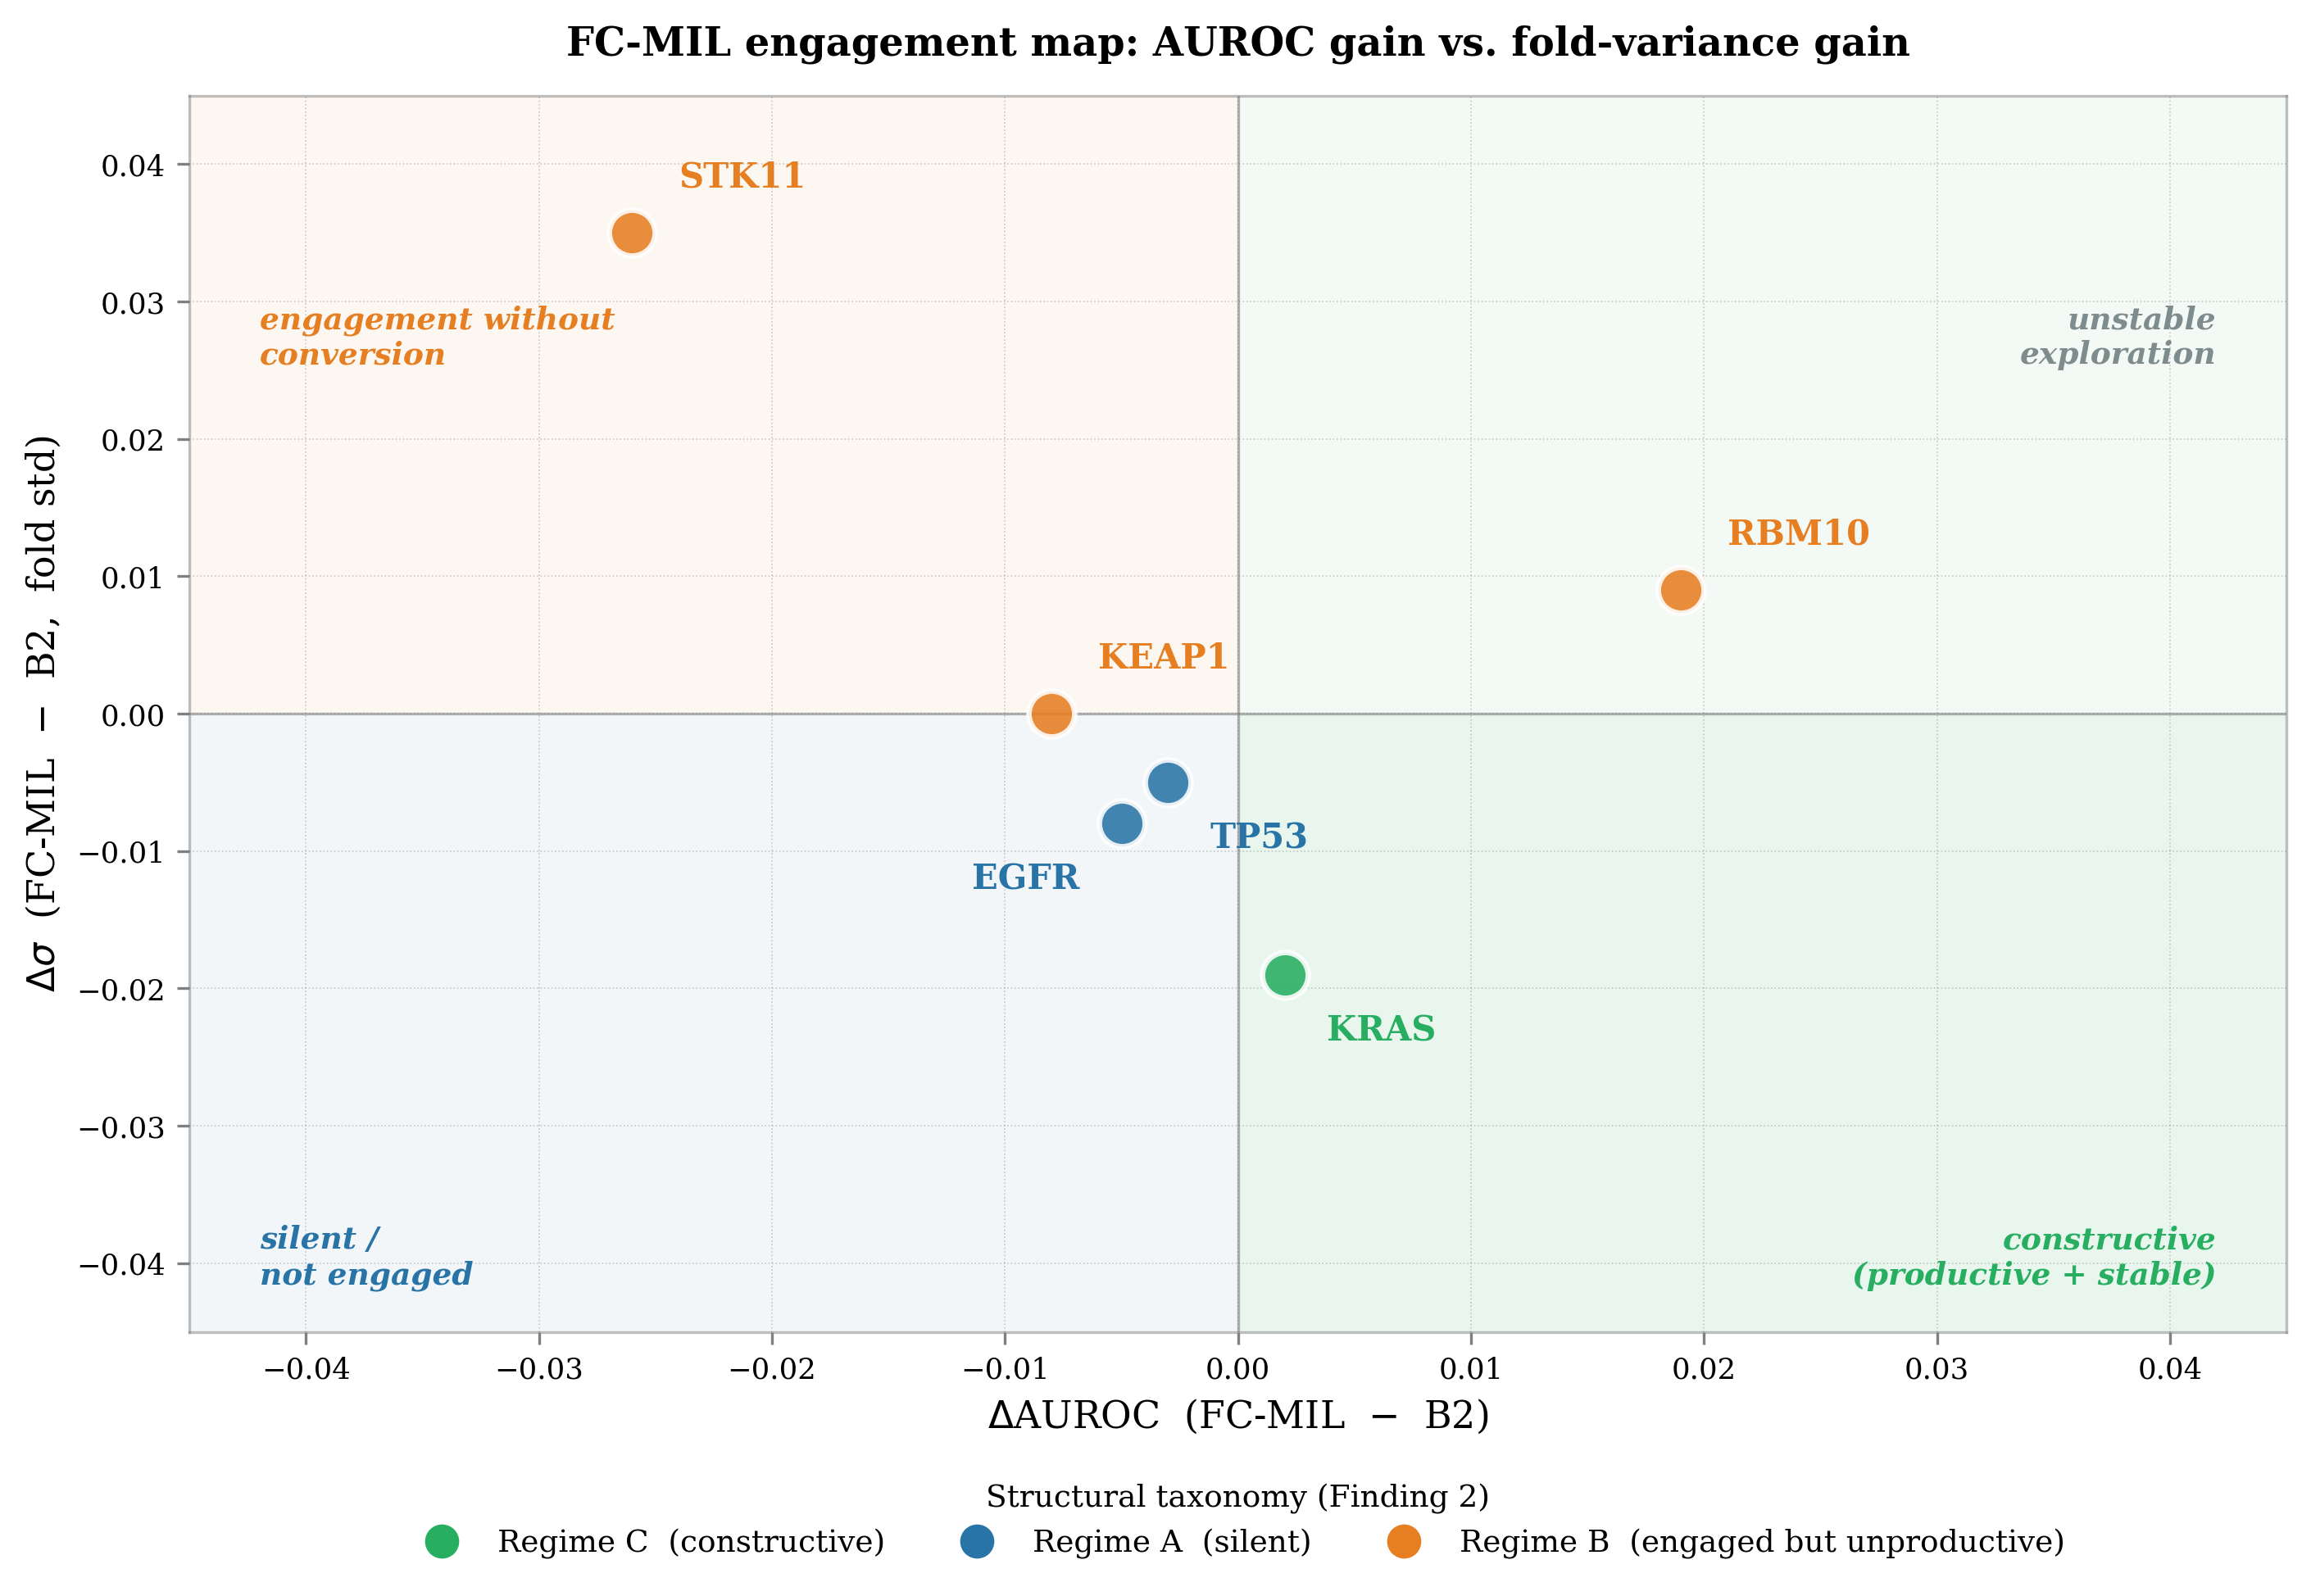
\includegraphics[width=\textwidth]{chapters/figures/choquet_variance_map.png}
  \caption[FC-MIL engagement map: AUROC gain $\times$
    fold-to-fold variance.]{%
    Per-gene scatter of $\Delta\mathrm{AUROC}$ (x) and $\Delta\sigma$
    across folds (y), both FC-MIL\,$-$\,B2
    (Table~\ref{tab:mutation_luad}).
    Marker colours follow Finding~2's structural taxonomy:
    \textcolor[HTML]{27AE60}{green}~$=$~regime~C constructive (KRAS);
    \textcolor[HTML]{2874A6}{blue}~$=$~regime~A silent (TP53, EGFR);
    \textcolor[HTML]{E67E22}{orange}~$=$~regime~B engaged-but-unproductive
    (STK11, KEAP1, RBM10).
    The four quadrants then distinguish productive vs.\ unproductive
    engagement of the Choquet branch:
    \emph{lower-right} = constructive / productive\,+\,stable (KRAS);
    \emph{upper-right} = unstable exploration (RBM10);
    \emph{upper-left} = engagement without conversion (STK11);
    \emph{lower-left} = silent / not engaged (TP53, EGFR; KEAP1
    sits near the origin in the upper-left quadrant).}
  \label{fig:choquet_variance_map}
\end{figure}

% ============================================================================
\section{Comparison with the Published Literature}
\label{sec:eval:literature}
% ============================================================================

This section interprets the results of this thesis against the
published mutation prediction literature surveyed in
Section~\ref{sec:bg:related:gap}
(Table~\ref{tab:literature_comparison}, which lists AUROCs for all
six target genes across Coudray, Kather, Saldanha, Logan, DeepGEM,
EAGLE, CHIEF, and this thesis).
The discussion below focuses on the three comparable-scale public
studies ($N < 1{,}000$) and on the structural gap to large-scale
proprietary studies.

\textbf{Key comparisons at matched scale:}

\begin{itemize}
    \item \textbf{vs.\ Coudray et al.\ (2018):} Coudray's EGFR AUROC (0.826)
    and KRAS (0.733) exceed this thesis's results.
    However, Coudray used a single held-out test split of 62 slides (not
    cross-validation), an end-to-end Inception-v3 trained directly with
    mutation labels (no MIL), and a smaller LUAD-only cohort of 382 slides.
    Single-split evaluation on 62 slides is known to produce optimistic
    estimates.
    The methodological contribution of this thesis---pattern-informed
    interpretability with rigorous cross-validation---trades some apparent
    discriminative performance for reproducibility and clinical verifiability.

    \item \textbf{vs.\ Saldanha et al.\ (2023):} The B2 condition
    of this thesis outperforms Saldanha for TP53 (0.718 vs.\
    $\sim$0.65) and EGFR (0.701 vs.\ $\sim$0.67) on a comparable
    cohort (687 vs.\ 676 slides);
    for KRAS, the thesis's top result is achieved by FC-MIL
    ($0.609$; Table~\ref{tab:mutation_luad}), essentially on par
    with Saldanha's $\sim 0.61$, while B2 alone reaches $0.607$.
    Several methodological differences confound a clean attribution:
    (i)~the encoder backbone (CTransPath, a Swin Transformer
    pretrained on $\sim$15M histopathology
    tiles~\cite{wang2022ctranspath}, vs.\ RetCCL, a ResNet-50
    contrastive model~\cite{wang2023retccl});     (ii)~the embedding
    dimensionality (512-d vs.\ 2048-d), which is favourable under
    data scarcity (sample-complexity argument); and (iii)~the
    domain-specific fine-tuning of CTransPath with FuzzyArcLoss~V2
    on the six LUAD patterns (Artefact~1,
    Section~\ref{sec:meth:pattern_classifier}), which orients the
    embedding geometry around morphological distinctions relevant
    to LUAD.
    The relative contribution of (i)--(iii) is not isolated by
    any ablation in this thesis and would require a direct B2 run
    on raw (non-fine-tuned) CTransPath embeddings or on RetCCL
    embeddings to disentangle.
    What the comparison \emph{does} establish is that the
    pattern-oriented embedding pipeline is competitive at matched
    public-data scale.

    \item \textbf{vs.\ Logan et al.\ (2022):} The B2 condition
    reports TP53 $0.718$ and EGFR $0.701$ versus Logan's $0.692$
    and $0.681$ at comparable scale (687 vs.\ 747 slides).
    The differences ($+0.026$ TP53, $+0.020$ EGFR) are smaller than
    the per-fold standard deviation observed in this thesis
    ($\sigma \approx 0.04$--$0.09$;
    Table~\ref{tab:mutation_luad}), so the two studies are best
    read as \emph{statistically comparable} rather than as one
    surpassing the other.
    The cohorts also differ: Logan evaluates on DHMC and CPTAC-3
    (no TCGA), and the absence of paired fold-level scores
    precludes a direct significance test.
    What \emph{is} notable is that Logan's auxiliary
    subtype-distribution features are conceptually adjacent to the
    pattern-informed approach of this thesis: both inject
    histological-class information into a mutation predictor.
    Logan's results therefore corroborate the broader hypothesis
    that pattern/subtype information is useful for mutation
    prediction, without being a controlled validation of the
    specific PI-ABMIL or FC-MIL designs.
\end{itemize}

\textbf{Regarding large-scale studies:}
The AUROCs of 0.82--0.96 reported by DeepGEM (3,637 patients from 16
hospitals) and 0.890 by EAGLE (8,461 slides) represent a different
data regime entirely (values as published; see
Table~\ref{tab:literature_comparison} in
Section~\ref{sec:bg:related:gap}).
These results reflect the advantage of massive proprietary clinical data
rather than a methodological superiority.
No publicly available dataset exceeds $\sim$897 LUAD cases
(Section~\ref{sec:uc:data_scarcity}); the performance gap is therefore
structural and not closable within the scope of any thesis relying on
public data.


% ============================================================================
% REWRITTEN SECTION — Chapter 6: sec:eval:interpretability
% Replaces the placeholder/hypothetical text with real observations
% from the 36 trained attention map figures (6 genes × 3 TP + 3 TN)
% generated using real ABMIL checkpoints from the patched benchmark run.
%
% Figures referenced (place in figures/attention_maps_v2/{GENE}/):
%   TP53:  TP_rank1_TCGA-99-8025-01A-01-.png
%          TN_rank1_TCGA-49-4510-01Z-00-.png
%   EGFR:  TP_rank1_TCGA-86-8280-01A-01-.png
%   KRAS:  TP_rank1_TCGA-55-7815-01A-01-.png
%   STK11: TP_rank1_TCGA-49-AAR0-11A-01-.png
%   KEAP1: TP_rank1_TCGA-49-AAR9-01Z-00-.png
%
% Also updated: sec:eval:lchai (36 slides, real checkpoints)
% ============================================================================


% ============================================================================
\section{Interpretability Analysis}
\label{sec:eval:interpretability}
% ============================================================================

This section presents the qualitative interpretability evidence for the
PI-ABMIL approach (RQ4), based on attention maps
generated from the trained model checkpoints.
Table~\ref{tab:viz_folds} reports the AUROC values used by LCHAI~v2.0
for Conclusive/Inconclusive labelling.
By design, LCHAI uses the \emph{5-fold mean AUROC} rather than the
best single-fold AUROC.
This is a deliberate conservative choice grounded in statistical
generalisability: the mean of five held-out test folds is an estimator
of the \emph{expected performance on any unseen patient from the
same population}.
Each fold evaluates a different 20\% of patients that the model never
saw during training; averaging these five estimates converges toward
the true population-level AUROC.
In contrast, the best fold AUROC reflects a single favourable data
partition---it indicates what the model \emph{can} achieve under
ideal conditions but may overestimate performance for the next
patient, who may resemble the worst fold rather than the best.
For a clinical decision-support tool, conservative estimates are
preferable: a clinician who trusts a label based on inflated AUROC
may forgo molecular testing that would have been warranted.
For transparency, the best fold AUROC is reported alongside the mean
to show the performance ceiling and to motivate future work with
larger cohorts where the gap between mean and best narrows.

\begin{table}[ht!]
\centering
\small
\caption{AUROC values for the six target genes.
LCHAI~v2.0 uses the \emph{Mean AUROC} (5-fold average, bold) for
Conclusive/Inconclusive labelling ($\geq 0.70$ = Conclusive,
following the Hosmer--Lemeshow criterion~\cite{hosmer2000applied}).
The best single-fold AUROC is shown for reference.}
\label{tab:viz_folds}
\begin{tabular}{l c c l}
\hline
\textbf{Gene} & \textbf{Mean AUROC (used)} & \textbf{Best fold AUROC} & \textbf{Label} \\
\hline
TP53  & \textbf{0.718} & 0.793 & Conclusive \\
EGFR  & \textbf{0.701} & 0.758 & Conclusive \\
KRAS  & \textbf{0.609} & 0.684 & Inconclusive \\
STK11 & \textbf{0.695} & 0.727 & Inconclusive \\
KEAP1 & \textbf{0.610} & 0.737 & Inconclusive \\
RBM10 & \textbf{0.661} & 0.733 & Inconclusive \\
\hline
\end{tabular}
\end{table}


\subsection{Attention Maps with Pattern Overlay}
\label{sec:eval:interp:attention}

The LCHAI~v2.0 six-level interpretability framework provides, for each
slide, complementary visualisations presented
in Figures~\ref{fig:attn_tp53_tp}--\ref{fig:attn_rbm10_tp}:

\begin{itemize}
    \item \textbf{Pattern overlay} (left panel in each figure): maps
    every extracted tile to one of the six ANORAK-annotated growth patterns using a
    categorical colour code consistent with LCHAI~v2.0 (green~= micropapillary,
    red~= acinar, dark red~= solid, cyan~= cribriform, yellow~= papillary,
    blue~= lepidic), providing a spatial view of tumour heterogeneity.\footnote{Pattern names and colours follow the Zenodo--ANORAK scheme (Section~\ref{sec:uc:zenodo}). A preliminary expert review of TCGA slides by a board-certified pathologist from SOLCA Ecuador is reported in Section~\ref{sec:eval:pattern:confusion}; a formal multi-rater concordance study remains as future work (Section~\ref{sec:eval:lim:data}).}

    \item \textbf{ABMIL attention map} (right panel): shows the
    continuous attention weights assigned by the gene-specific ABMIL
    model, with cyan semi-transparent regions and white contours
    delineating the tiles that contribute most to the mutation
    prediction.
\end{itemize}

Each figure is arranged in a $2 \times 2$ grid with four
complementary panels:

\begin{itemize}
    \item \textbf{Top left --- Pattern overlay}: spatial map of the six
    growth patterns.
    \item \textbf{Top right --- Attention map}: ABMIL attention weights
    showing which tiles drive the prediction.
    \item \textbf{Bottom left --- SHAP decomposition}: stacked bar
    showing the embedding/pattern attribution split (Level~3,
    Section~\ref{sec:meth:interp:shap}).
    \item \textbf{Bottom right --- Ablation comparison}: per-slide
    feature channel ablation (Level~5,
    Section~\ref{sec:meth:interp:ablation}), comparing the mutation
    probability produced by three separately trained models---Combined
    ($P_{\text{comb}}$), Embeddings-only ($P_{\text{emb}}$), and
    Patterns-only ($P_{\text{pat}}$)---on the same tile set.
    The ablation delta $\Delta_{\text{pat}} = P_{\text{comb}} -
    P_{\text{emb}}$ (Equation~\ref{eq:delta_pattern}) reveals whether
    adding pattern features helps ($\Delta > 0$) or hurts
    ($\Delta < 0$) the prediction on this specific slide.
\end{itemize}

The top panels reveal \emph{where} the model attends and \emph{what}
it finds there.
The bottom panels address a deeper question: SHAP (bottom left) shows
how the model \emph{distributes its internal attribution} between
embeddings and patterns, while ablation (bottom right) shows whether
patterns \emph{actually help or harm} the prediction
(cf.\ Section~\ref{sec:bg:channel_ablation}).
As the per-gene analyses below demonstrate, these two signals can
diverge dramatically.

All visualisations in this section were generated by LCHAI~v2.0
deployed at \url{https://lchai.gptfy.biz}.

\textbf{SHAP reproducibility note.}
DeepSHAP is an approximation that uses sampled background baselines,
so the exact percentage attributed to the embedding pathway versus
the pattern pathway varies by $\pm 5$--$10$ percentage points
between runs on the same slide.
The qualitative conclusion (which pathway dominated the prediction)
is stable.
The percentages reported in this section and in
Table~\ref{tab:enrichment_summary} come from a single deterministic
run with \texttt{seed=42} to allow exact reproduction; running the
analysis with a different seed will produce slightly different
numbers but the same dominance ordering.

\textbf{Conclusive vs Inconclusive labelling: what is
population-level and what is slide-level.}
Throughout the case studies that follow, the
Conclusive/Inconclusive label attached to each prediction is a
\emph{population-level} property derived from the cohort mean 5-fold
AUROC ($\geq 0.70$ = Conclusive, following Hosmer--Lemeshow;
Table~\ref{tab:viz_folds}).
It is fixed before any specific slide is examined: TP53 and EGFR
are population-level Conclusive, while KRAS, STK11, KEAP1 and RBM10 are
population-level Inconclusive.
The slide-level evidence presented in each case study (per-slide
$P(\text{mut})$, SHAP decomposition, Choquet Shapley values,
ablation gaps, dual-route diagrams) does \emph{not} produce the
label; it explains the \emph{mechanism} by which the model
succeeds or fails on that gene's cohort, making the cohort AUROC
concrete on a representative slide.
This decoupling matters most for KRAS, where a confidently
predicted slide ($P(\text{mut}) = 0.965$) still inherits a
population-level Inconclusive label---which is the precise behaviour
the Conclusive/Inconclusive criterion is designed to enforce.


\subsubsection{TP53: High-Confidence Detection in a
Micropapillary-Classified Dominant Tumour}
\label{sec:eval:tcga:tp53}

Figure~\ref{fig:attn_tp53_tp} shows the LCHAI~v2.0 output for slide
TCGA-99-8025, a TP53-mutant case predicted with high confidence
(P(mut)~$= 0.951$, method: B2 embeddings; population-level: Conclusive,
cohort mean 5-fold AUROC~$= 0.718$; Table~\ref{tab:viz_folds}).
The pattern overlay reveals a slide dominated by micropapillary-classified morphology
(91.5\%), with minor acinar (6.27\%), cribriform (1.6\%), and solid
(0.56\%) components.
The ablation analysis shows that the embedding-only model outperforms
the combined model for TP53 (emb~$= 0.951$ vs.\ combined~$= 0.778$),
confirming that the CTransPath embeddings carry the dominant TP53
signal.
TP53 mutations are associated with solid and micropapillary
patterns in the literature~\cite{ahn2022tp53highgrade}; on this slide, solid is present at only 0.56\%
while micropapillary is the dominant class at 91.5\%.
The model detects TP53 via sub-cellular texture (61\% embedding SHAP;
fuzzy classification: \emph{Balanced}). This is consistent with the
visual fingerprint that Mendoza~et~al.~\cite{mendoza2024tp53nuclear}
document for TP53-mutant LUAD: nuclei that are enlarged, vary
strongly in size and shape, stain darker than normal, and have wavy
or irregular borders. These cues live at the cell-and-nucleus scale
rather than at the tissue-architecture scale, so they are picked up
by the CTransPath embeddings rather than by the pattern channel.
The ablation comparison (bottom right of Figure~\ref{fig:attn_tp53_tp})
confirms this: the embeddings-only model (95.1\%) outperforms the combined
model (79.0\%), indicating that adding pattern features introduces
interference rather than complementary signal for TP53.

\begin{figure}[ht!]
\centering
\begin{minipage}[t]{0.48\textwidth}
\centering
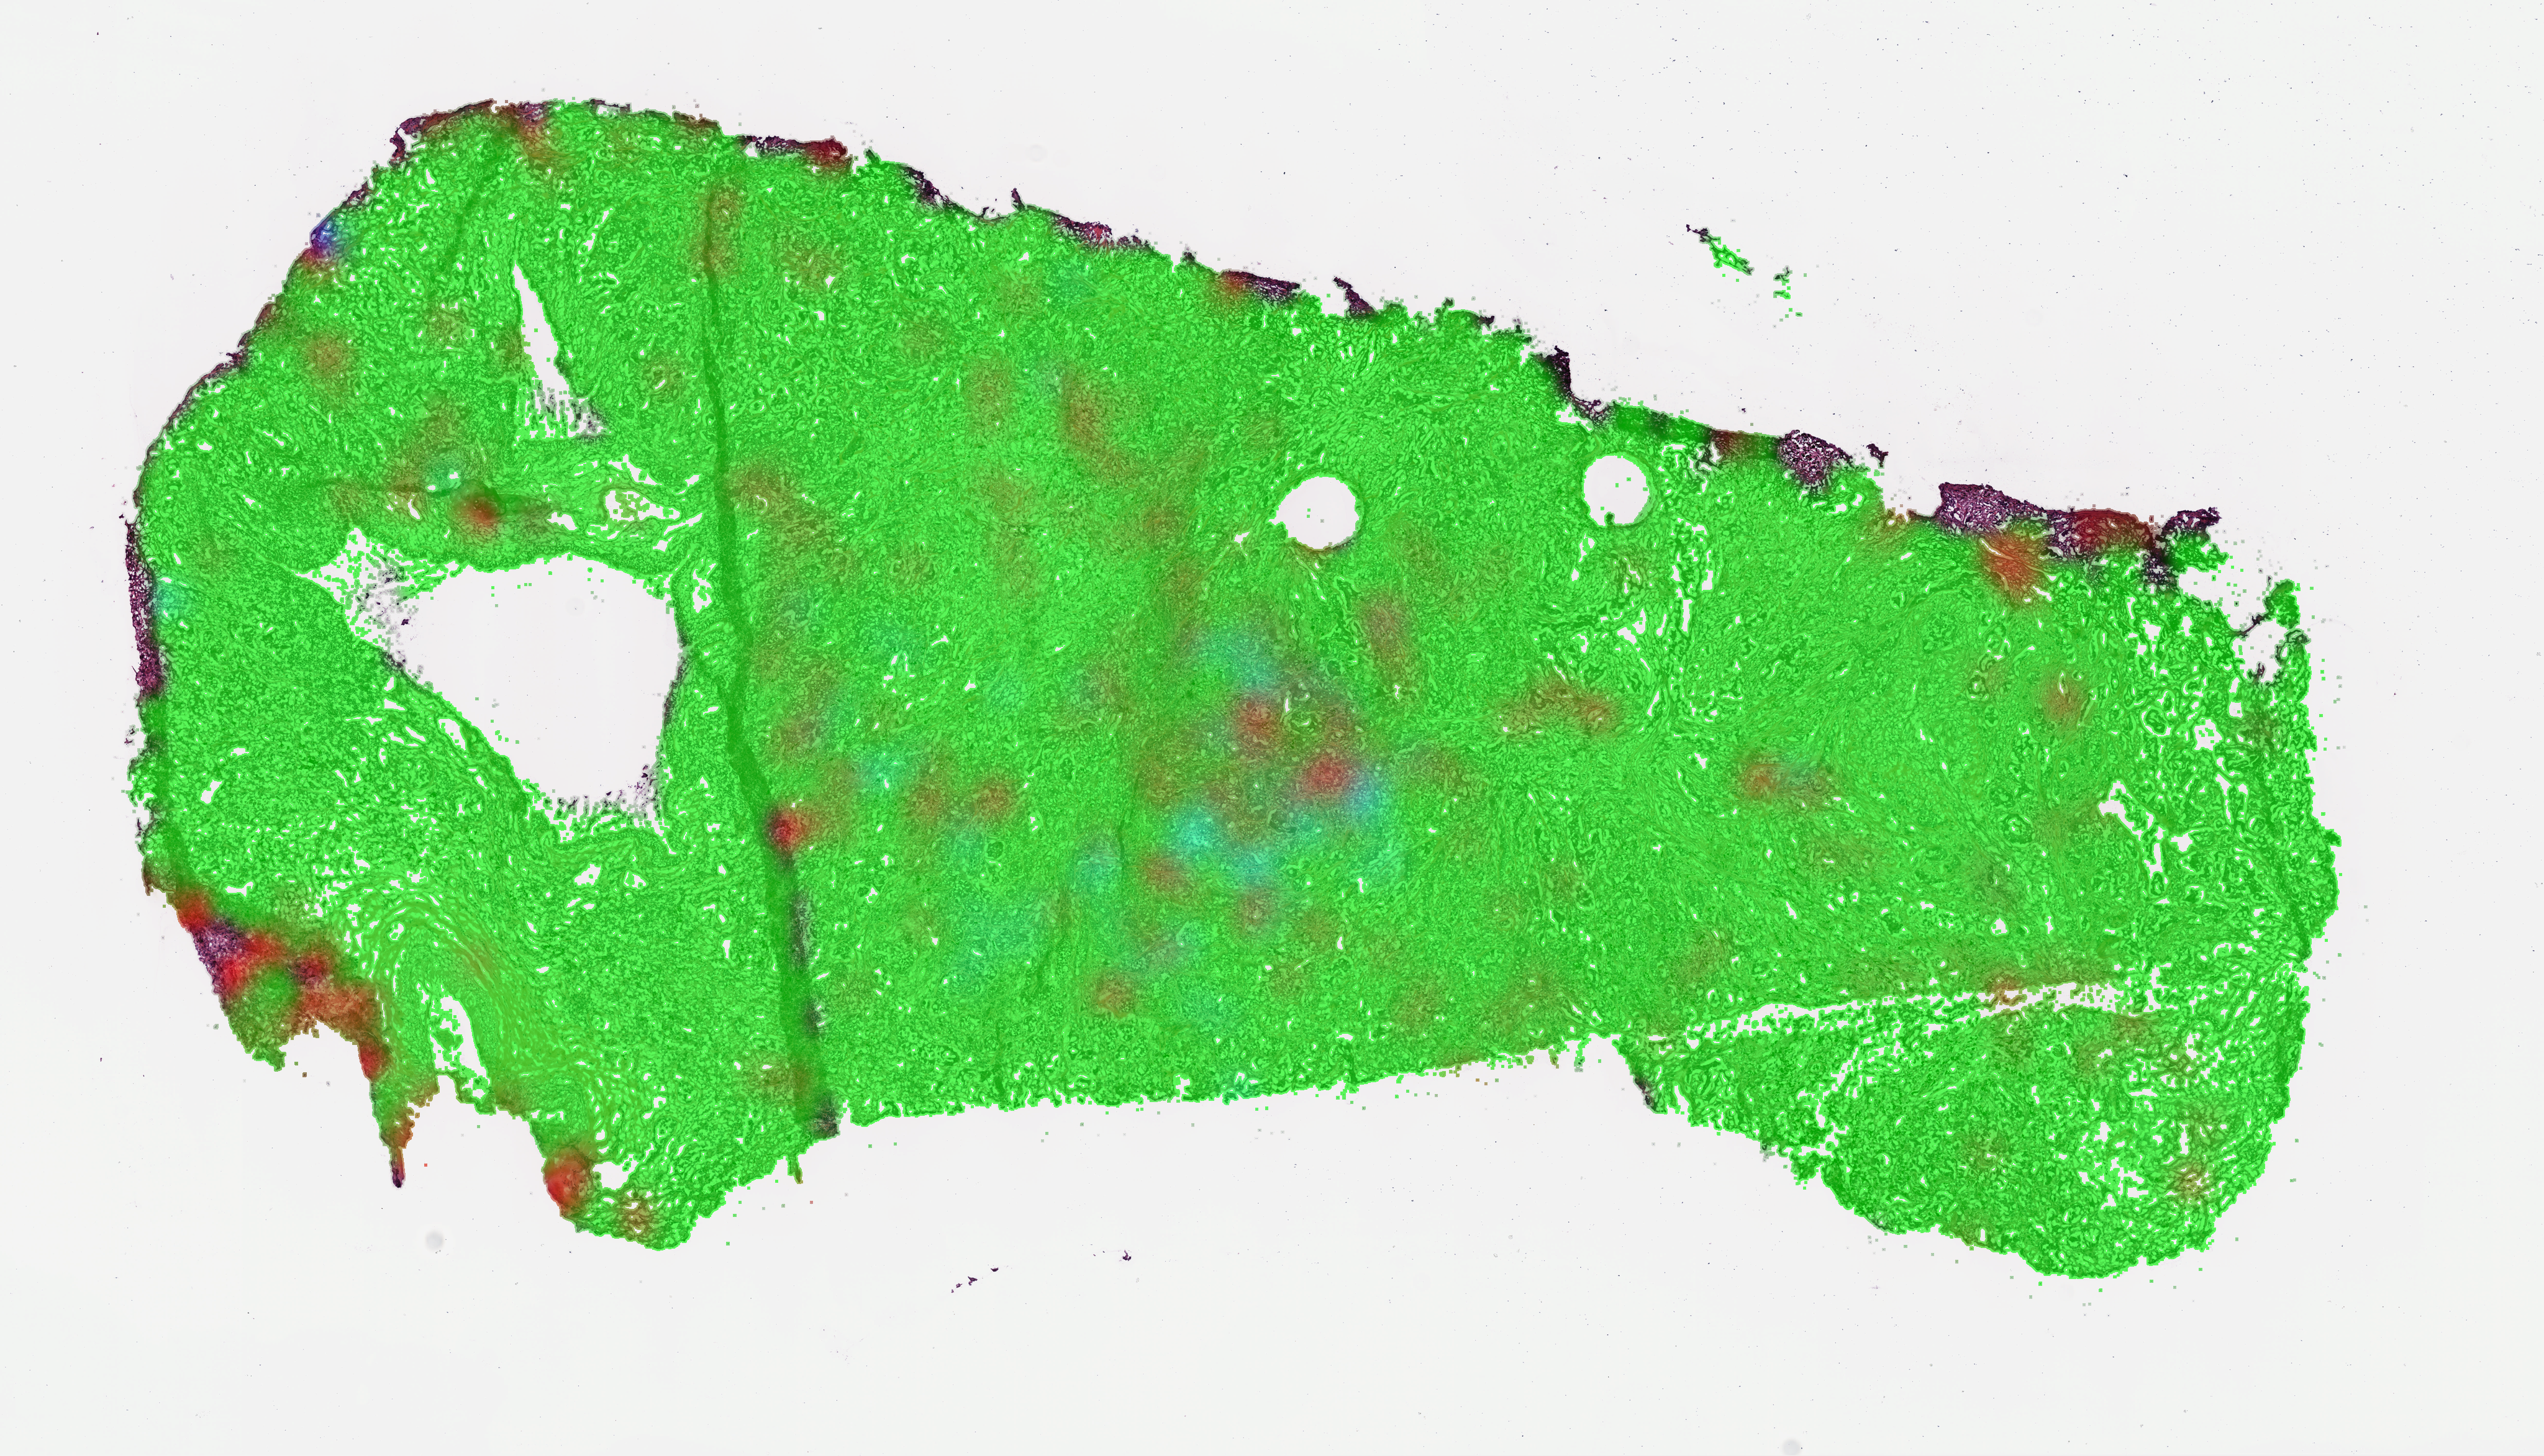
\includegraphics[width=\textwidth]{chapters/figures/lchai_v2_TP53_TCGA-99-8025_pattern_overlay.png}
\end{minipage}\hfill
\begin{minipage}[t]{0.48\textwidth}
\centering
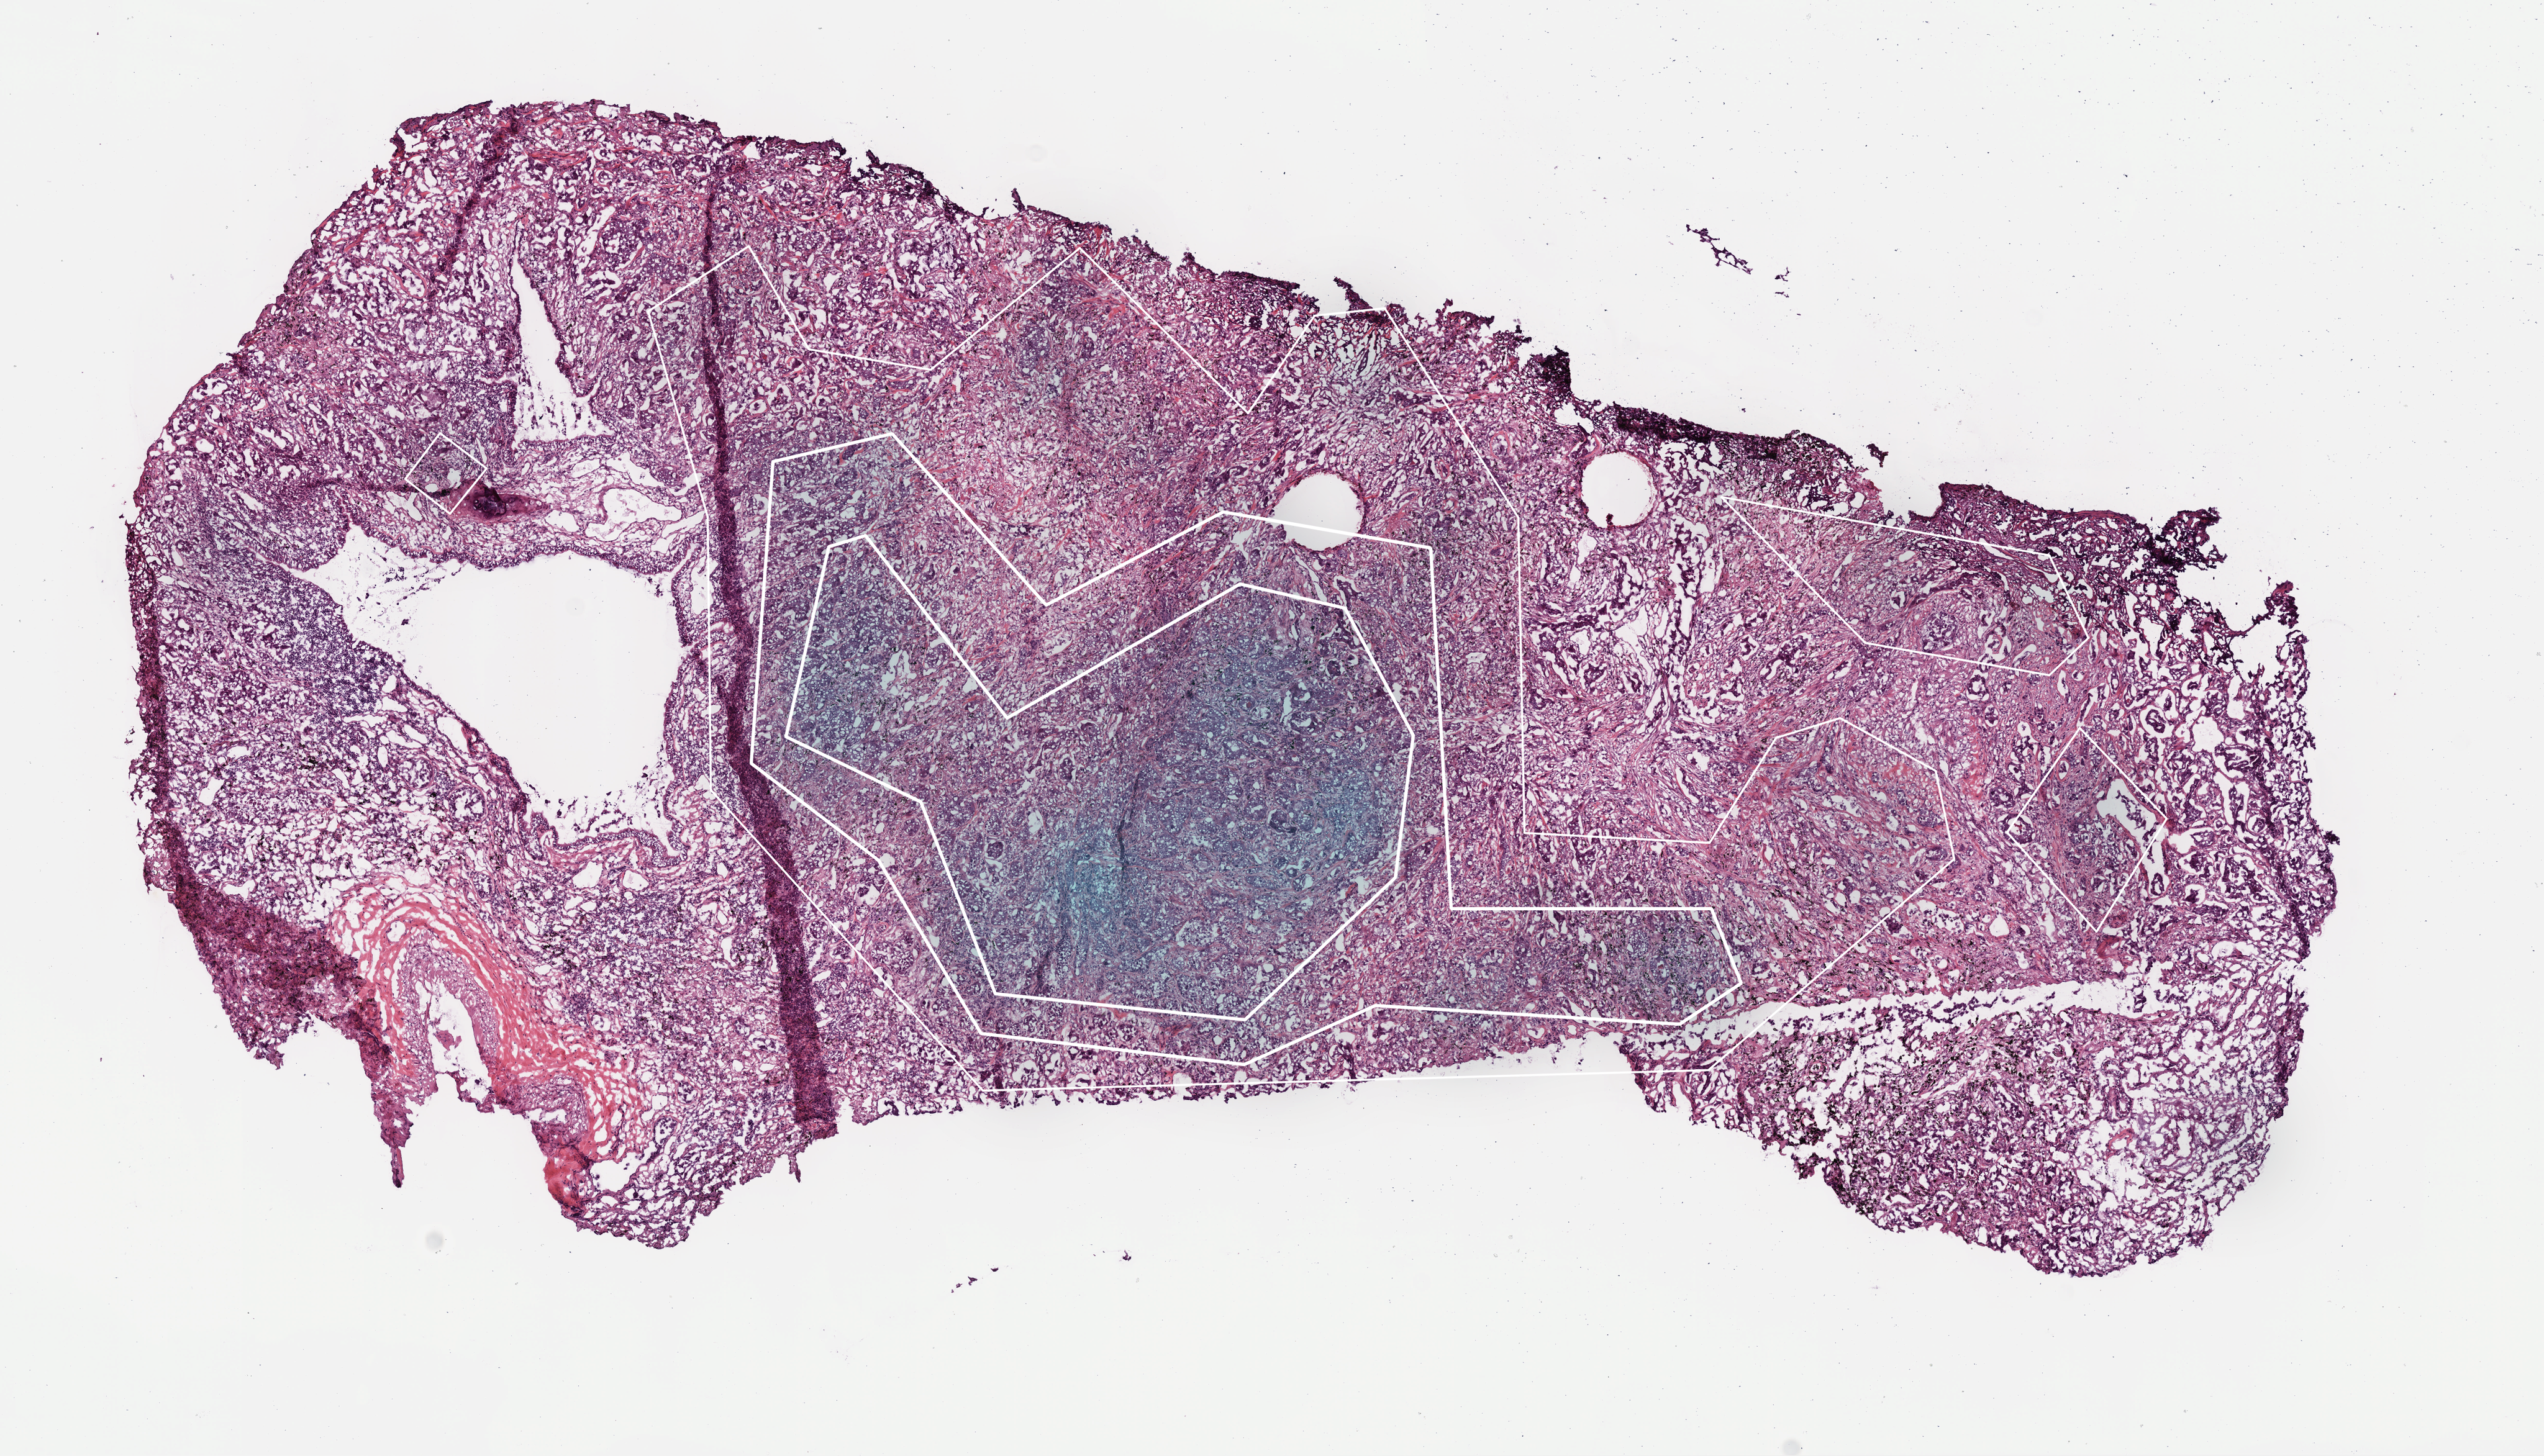
\includegraphics[width=\textwidth]{chapters/figures/lchai_v2_TP53_TCGA-99-8025_attention_map.png}
\end{minipage}\\[6pt]
\begin{minipage}[t]{0.48\textwidth}
\centering
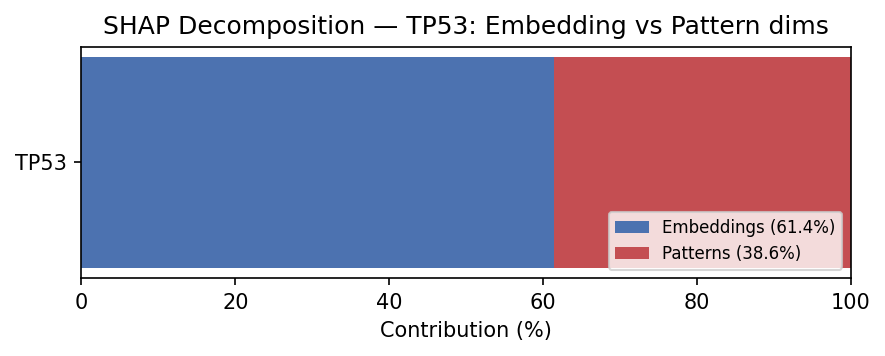
\includegraphics[width=\textwidth]{chapters/figures/shap_decomp_TP53_99_8025_bar.png}
\end{minipage}\hfill
\begin{minipage}[t]{0.48\textwidth}
\centering
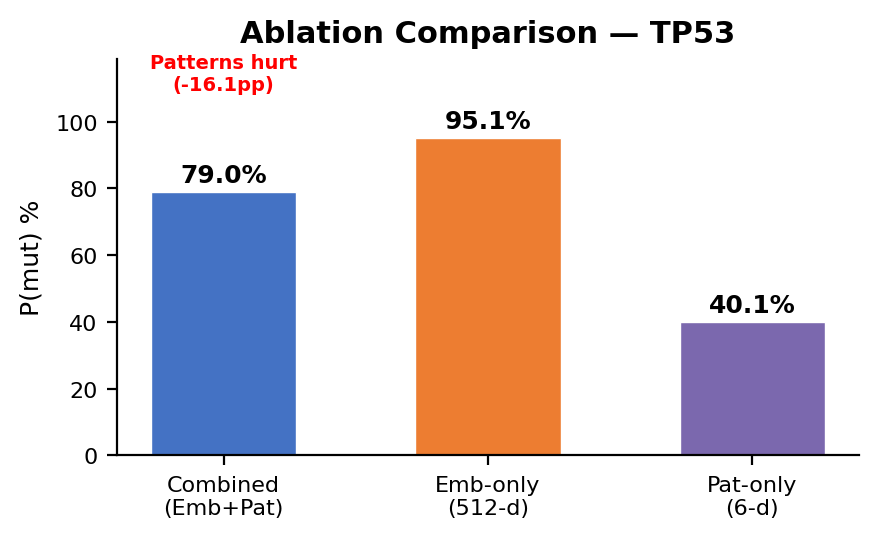
\includegraphics[width=\textwidth]{chapters/figures/ablation_TP53_99_8025.png}
\end{minipage}
\caption[LCHAI~v2.0 interpretability: TP53 (TCGA-99-8025)]{%
    LCHAI~v2.0 interpretability for TP53-mutant slide TCGA-99-8025
    (P(mut)~$= 0.951$, B2 embeddings; population-level: Conclusive).
    \textbf{Top left}: Pattern overlay (green~= micropapillary 91.5\%).
    \textbf{Top right}: ABMIL attention map.
    \textbf{Bottom left}: SHAP decomposition---61\% embedding / 39\% pattern.
    \textbf{Bottom right}: Ablation comparison---Emb-only (95.1\%) outperforms
    Combined (79.0\%), confirming that patterns introduce interference for TP53.}
\label{fig:attn_tp53_tp}
\end{figure}

\textbf{Interpretation.}
TP53 is the most commonly mutated gene in LUAD and emits a
\emph{multi-scale} visual signal: at the architectural scale, it
favours the high-grade growth patterns solid and
micropapillary~\cite{ahn2022tp53highgrade}; at the sub-cellular
scale, it produces visible nuclear changes---enlarged,
irregularly shaped, darker-staining nuclei (the histopathology
literature labels this \emph{nuclear pleomorphism})~\cite{mendoza2024tp53nuclear}.
Each scale reaches the network through a different input channel,
with very different effective bandwidth:
the pattern channel is a $6$-dimensional WHO-class probability
vector aggregated per tile, while the embedding channel is the
$512$-d projection of the $768$-d CTransPath embedding that
retains fine-grained texture
(Table~\ref{tab:tile_representations}).
On TCGA-99-8025 the architectural fingerprint is only
\emph{partially} present---the slide is $91.5\%$ micropapillary
but solid is essentially absent ($0.56\%$)---whereas the
sub-cellular fingerprint is distributed across the slide and is
the channel CTransPath was pretrained to capture.
The SHAP decomposition attributes $61\%$ of the prediction to the
embedding channel, and the model returns $P(\text{mut}) = 0.951$:
a high-confidence true positive driven by sub-cellular cues
rather than by the overall tissue layout.

The ablation comparison sharpens this reading.
The embeddings-only ablation reaches $95.1\%$, while adding the
pattern channel drops the prediction to $79.0\%$---a
$-16.1$\,pp pattern penalty (ablation panel in
Figure~\ref{fig:attn_tp53_tp}).
In engineering terms, \textbf{the deployed model would predict
TP53 \emph{better} if the pattern channel were ablated at
inference time on this slide}: the pattern channel is consulted,
but its contribution to the final probability is negative.
This is a clean instance of a recurring divergence in this
chapter, between \emph{feature attribution} (SHAP, which measures
how much each input channel \emph{moves} the model's output) and
\emph{causal contribution} (ablation, which measures whether the
channel's presence improves the prediction at all).
$39\%$ SHAP attribution to the pattern channel does not mean
patterns help---it means the prediction is sensitive to them,
and on this slide that sensitivity points the wrong way.
Figure~\ref{fig:tp53_two_scales} summarises the argument
geometrically: the TP53 signal lives at two spatial scales, each
routed through a distinct channel; on this slide only the
sub-cellular route carries useful evidence, while the pattern
channel attracts attribution but degrades the output.

\begin{figure}[H]
\centering
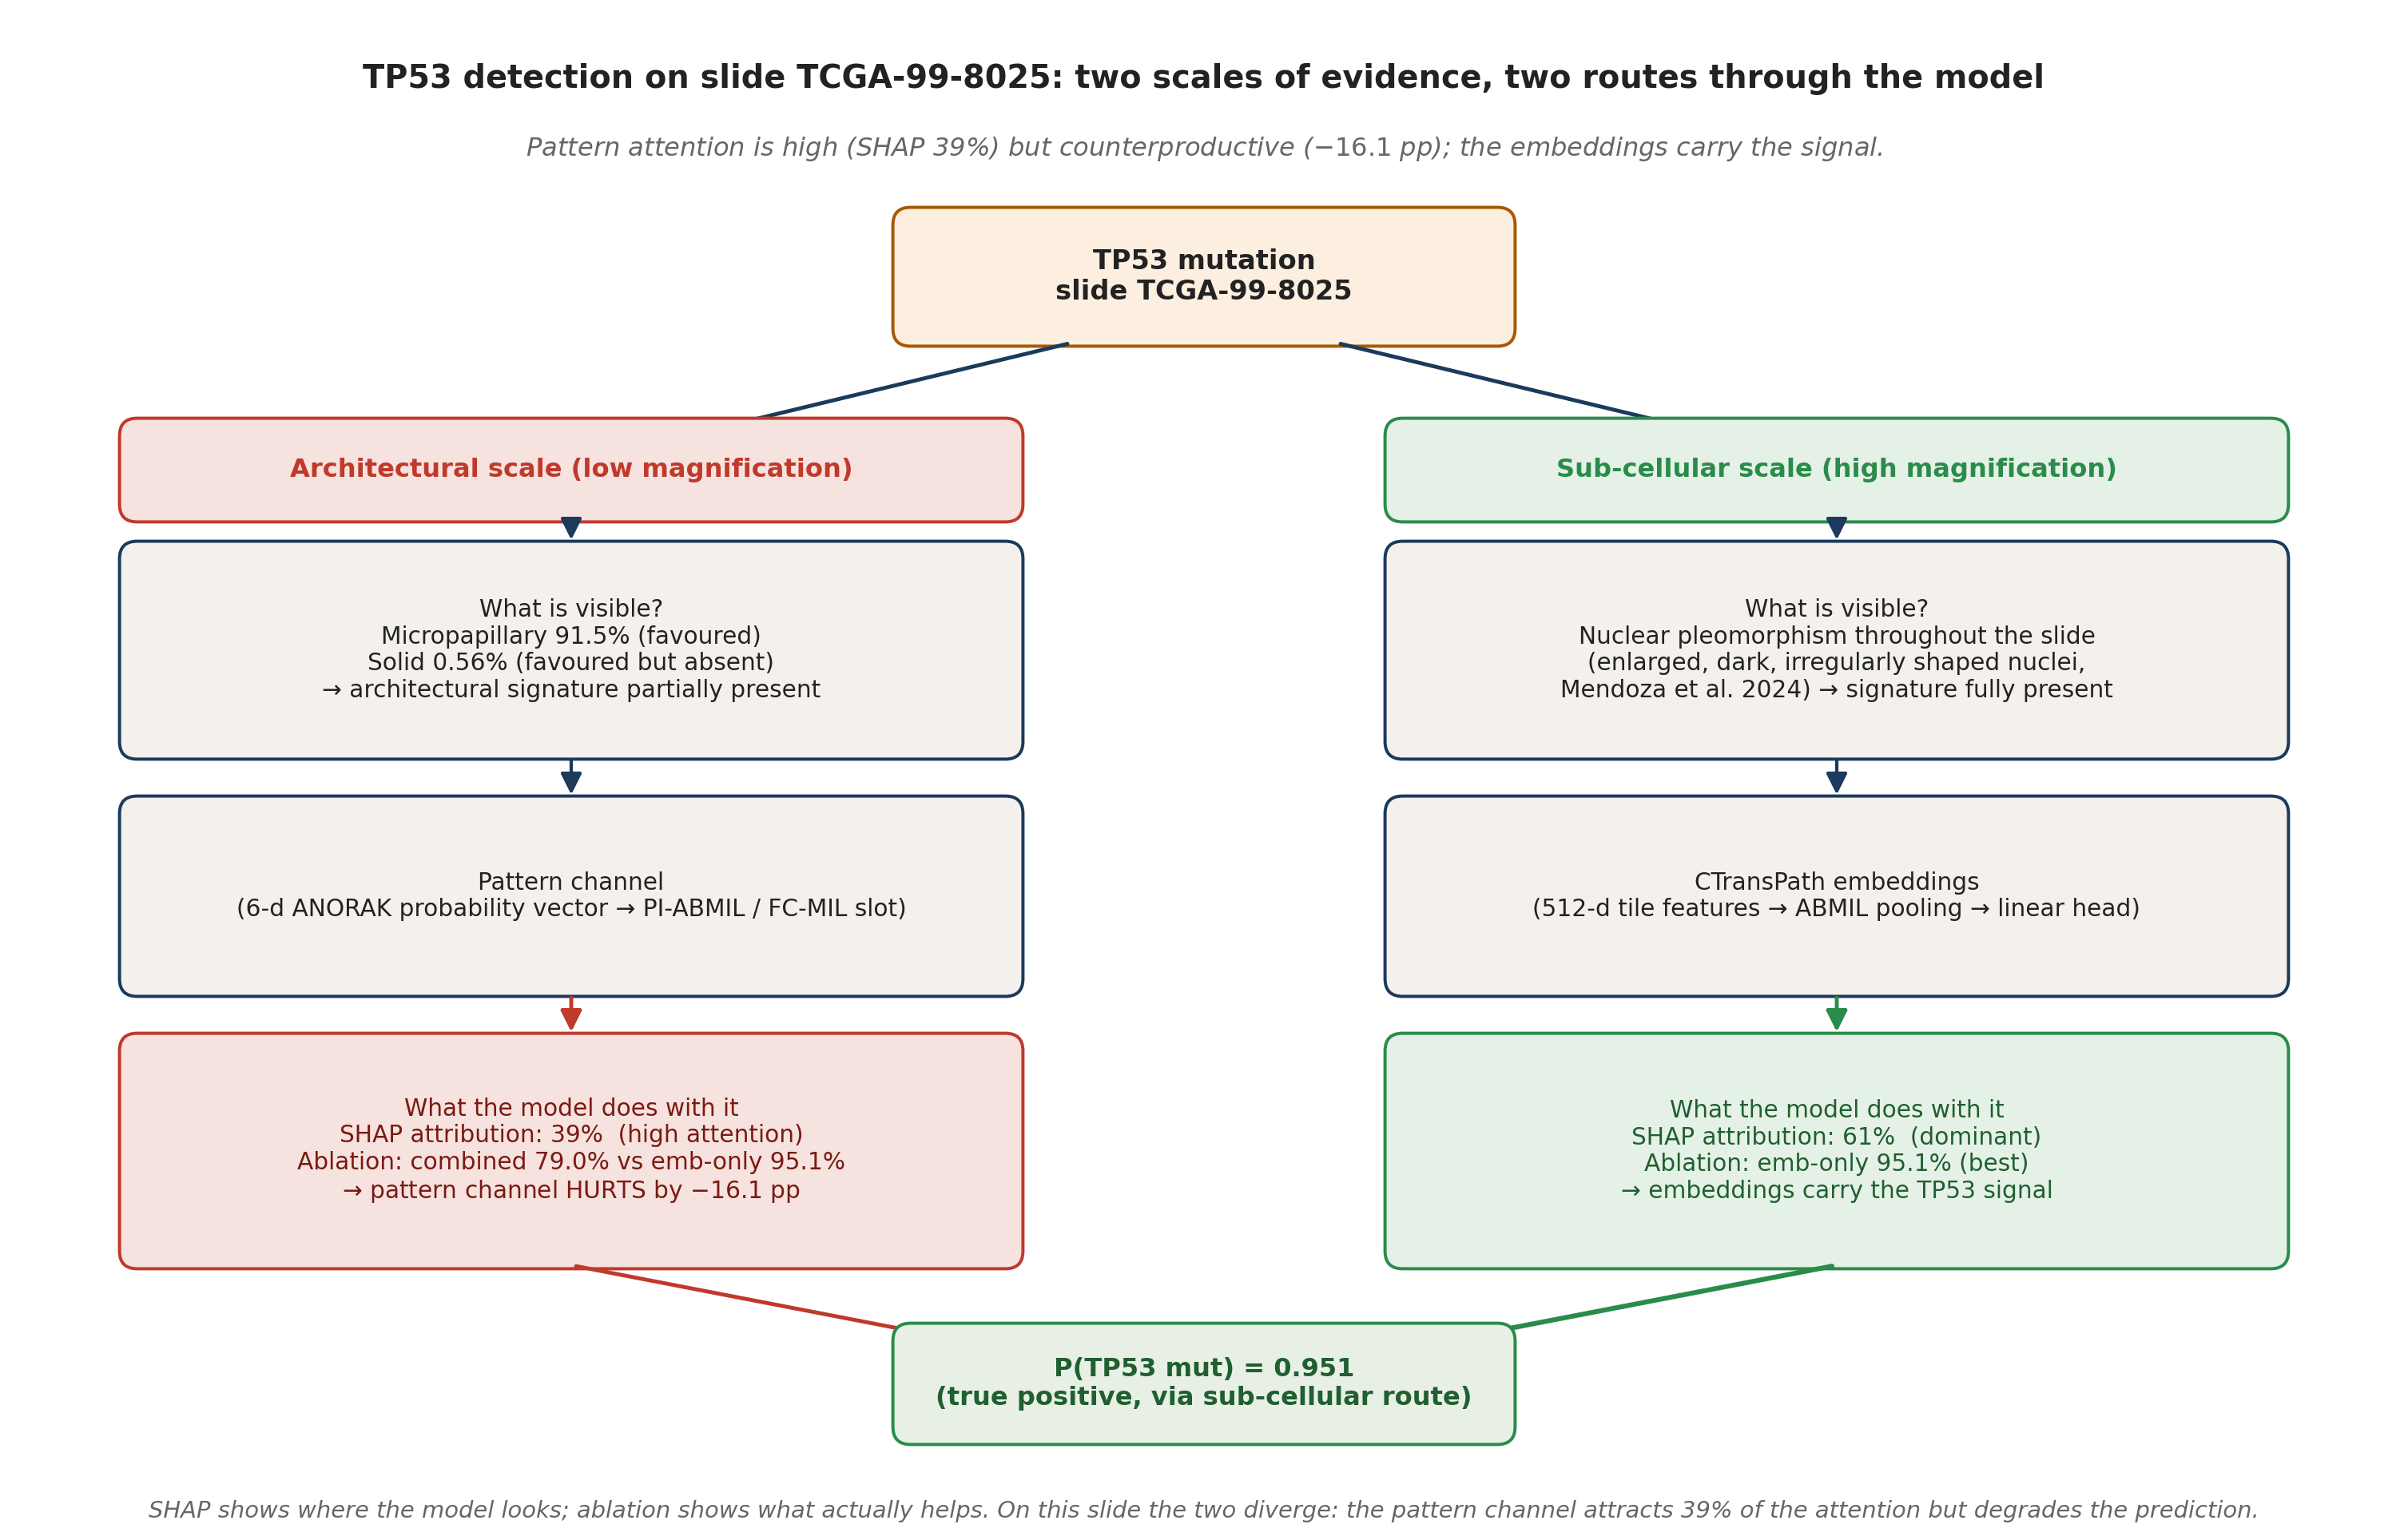
\includegraphics[width=\textwidth]{chapters/figures/tp53_two_scales.png}
\caption[TP53 detection on TCGA-99-8025: two scales, two routes]{%
    Visual summary of the TP53 interpretation for slide
    TCGA-99-8025.
    TP53 mutations leave traces at two scales: an
    \emph{architectural} scale (favoured high-grade growth
    patterns~\cite{ahn2022tp53highgrade}) and a \emph{sub-cellular}
    scale (nuclear pleomorphism: enlarged, dark, irregularly shaped
    nuclei~\cite{mendoza2024tp53nuclear}).
    On this slide the architectural signature is only partially
    present (micropapillary $91.5\%$ but solid $0.56\%$), while the
    sub-cellular signature is present throughout.
    The two scales reach the model through different channels: the
    pattern channel (6-d ANORAK probability vector) and the
    CTransPath embeddings (512-d tile features,
    Table~\ref{tab:tile_representations}).
    SHAP attributes $39\%$ of the prediction to the pattern channel,
    yet the ablation shows that this channel \emph{hurts} the
    prediction by $-16.1$\,pp (combined $79.0\%$ vs.\ emb-only
    $95.1\%$).
    The successful prediction (P~$=0.951$, true positive) flows
    through the sub-cellular route alone---a clear instance of the
    recurring divergence between \emph{what the model looks at}
    (SHAP) and \emph{what actually helps} (ablation).}
\label{fig:tp53_two_scales}
\end{figure}


\subsubsection{EGFR: Micropapillary-Dominant Morphology in a
Low-Probability Prediction}
\label{sec:eval:tcga:egfr}

Figure~\ref{fig:attn_egfr_tp} shows the LCHAI~v2.0 output for slide
TCGA-86-8280, an EGFR-mutant case predicted with low mutation
probability (P(mut)~$= 0.076$, method: B2 embeddings; population-level:
Conclusive, cohort mean 5-fold AUROC~$= 0.701$;
Table~\ref{tab:viz_folds}).
The slide exhibits a strongly micropapillary-dominant morphological profile:
micropapillary (94.94\%), solid (3.16\%), acinar (1.39\%),
lepidic (0.3\%), and cribriform (0.16\%).
Despite the homogeneous pattern composition, the model assigns a low
EGFR probability---a false negative.

\begin{figure}[ht!]
\centering
\begin{minipage}[t]{0.48\textwidth}
\centering
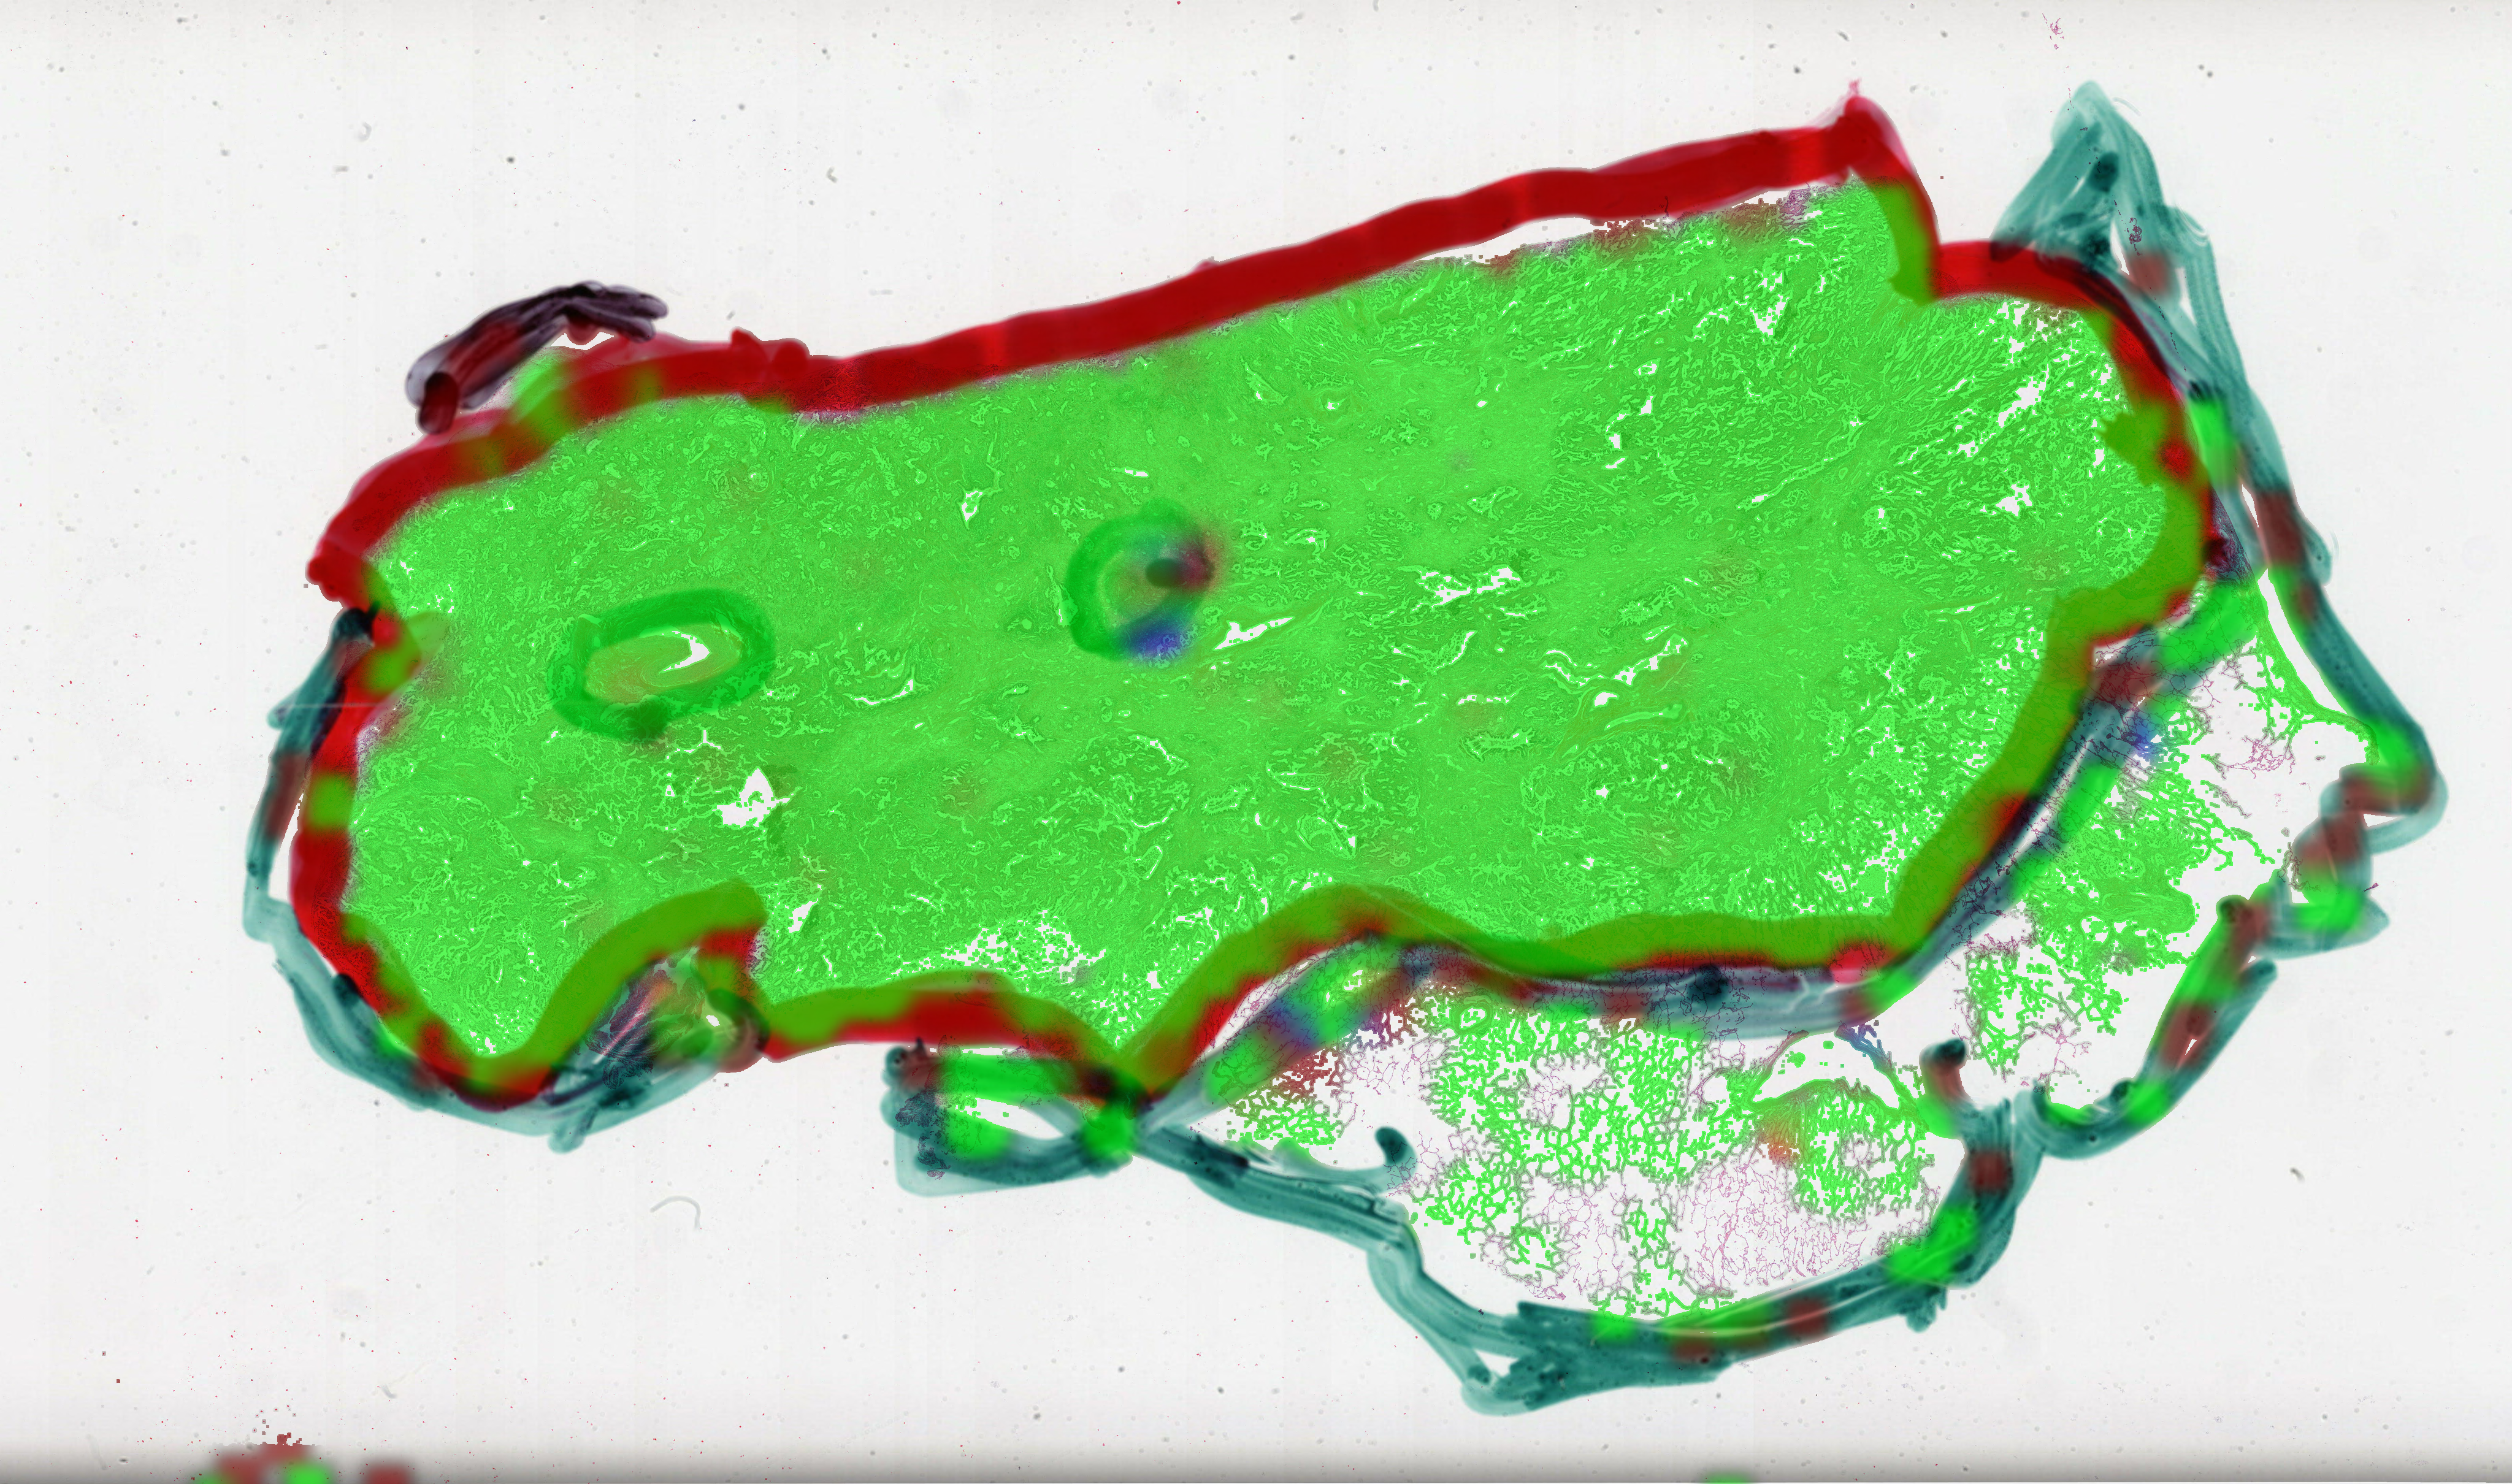
\includegraphics[width=\textwidth]{chapters/figures/lchai_v2_EGFR_TCGA-86-8280_pattern_overlay.png}
\end{minipage}\hfill
\begin{minipage}[t]{0.48\textwidth}
\centering
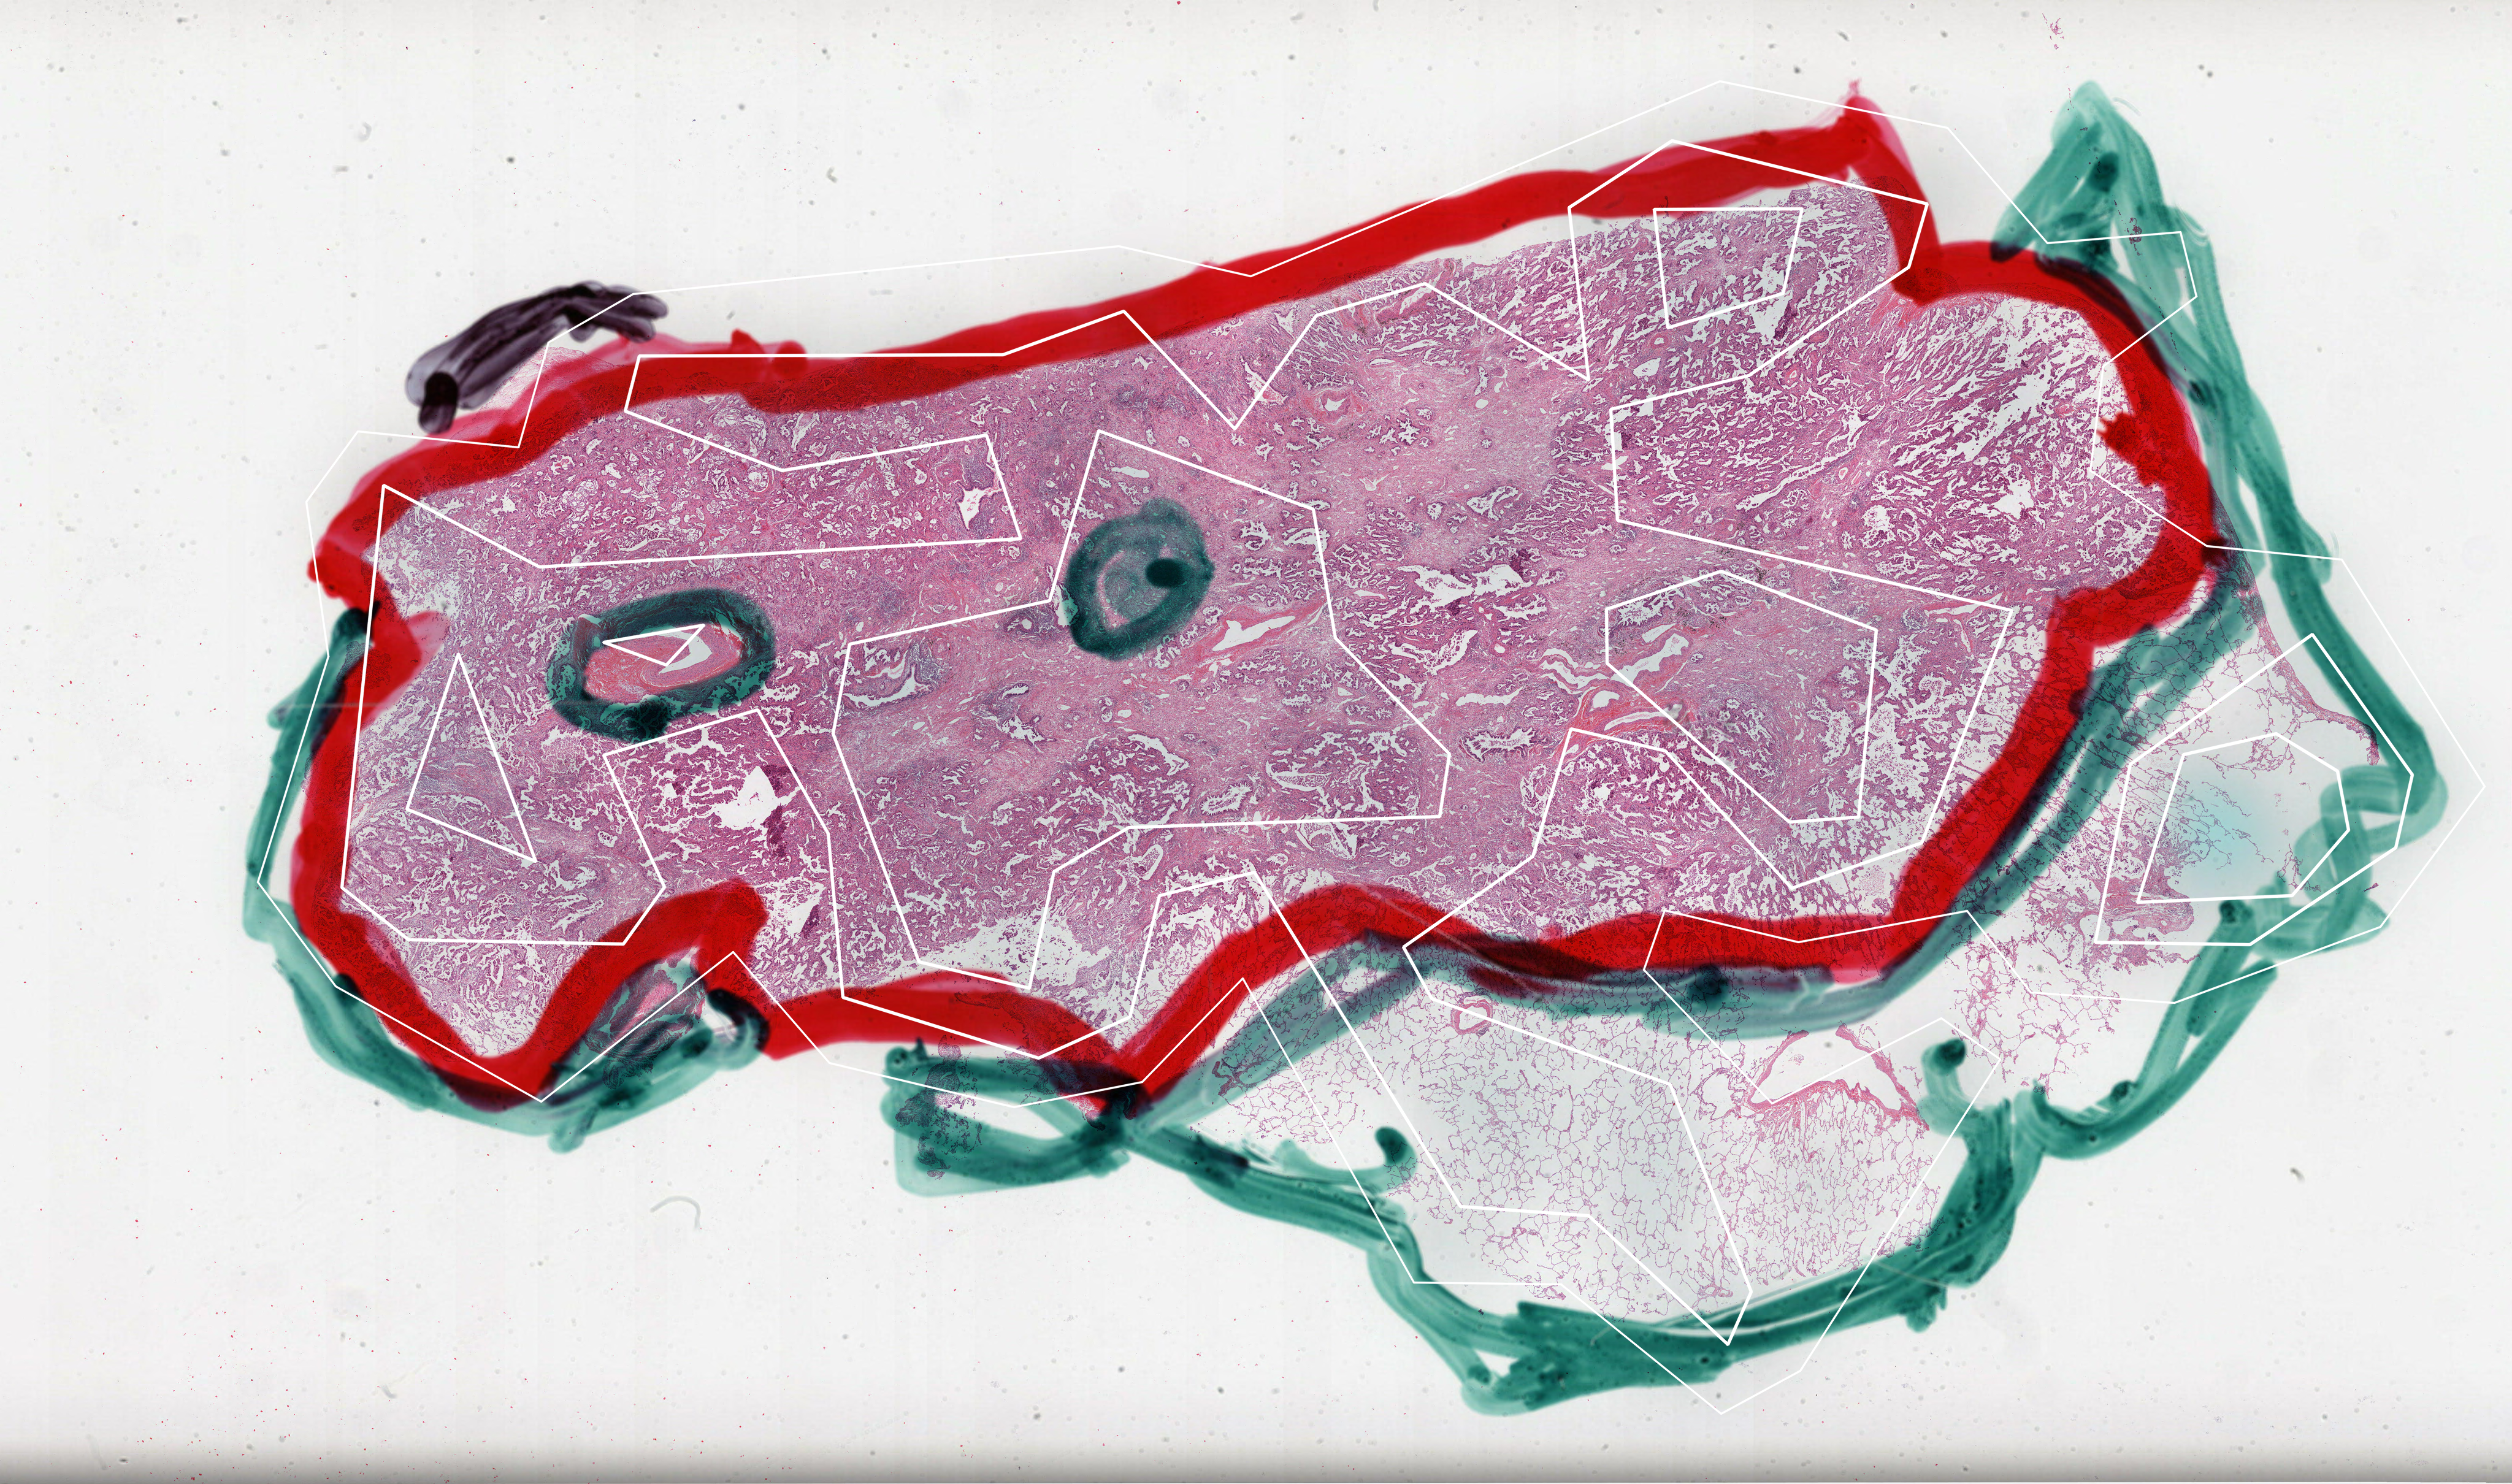
\includegraphics[width=\textwidth]{chapters/figures/lchai_v2_EGFR_TCGA-86-8280_attention_map.png}
\end{minipage}\\[6pt]
\begin{minipage}[t]{0.48\textwidth}
\centering
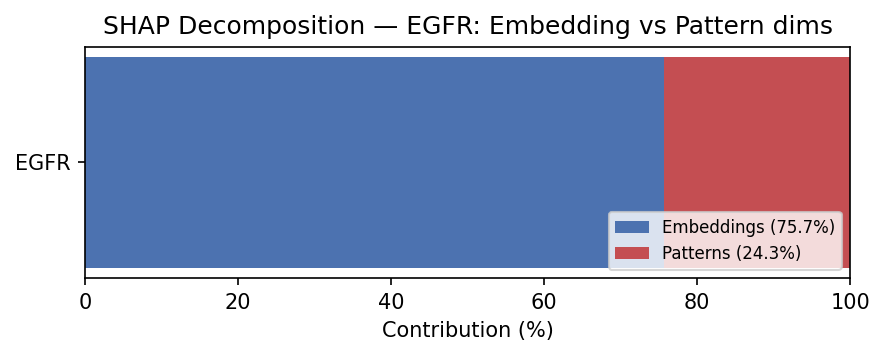
\includegraphics[width=\textwidth]{chapters/figures/shap_decomp_EGFR_86_8280_bar.png}
\end{minipage}\hfill
\begin{minipage}[t]{0.48\textwidth}
\centering
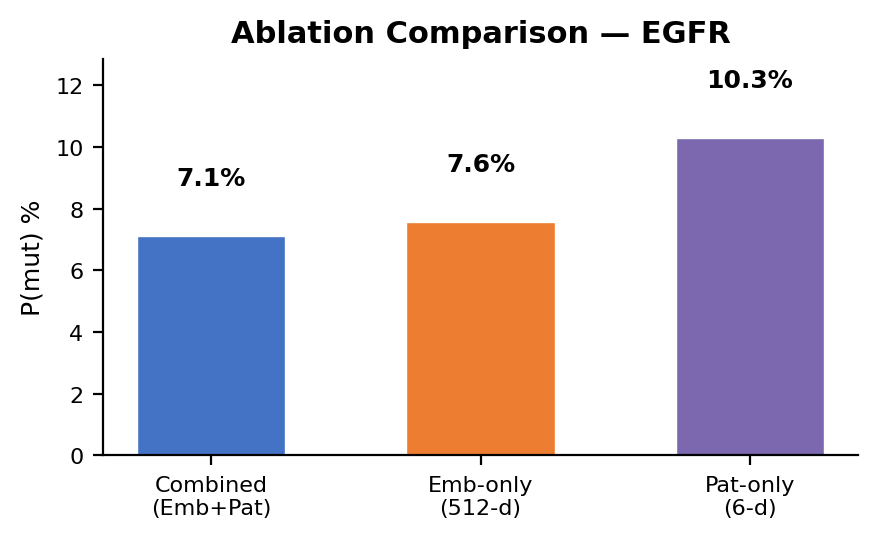
\includegraphics[width=\textwidth]{chapters/figures/ablation_EGFR_86_8280.png}
\end{minipage}
\caption[LCHAI~v2.0 interpretability: EGFR (TCGA-86-8280)]{%
    LCHAI~v2.0 interpretability for EGFR case TCGA-86-8280
    (P(mut)~$= 0.076$, B2 embeddings; population-level: Conclusive).
    \textbf{Top left}: Pattern overlay---micropapillary-dominant (94.94\%, green).
    \textbf{Top right}: ABMIL attention map.
    \textbf{Bottom left}: SHAP decomposition---76\% embedding / 24\% pattern.
    \textbf{Bottom right}: Ablation---all three models produce similarly low
    probabilities (7.1\%, 7.6\%, 10.3\%), confirming absent morphological signal.}
\label{fig:attn_egfr_tp}
\end{figure}

\textbf{Interpretation.}
This case illustrates a structural limitation of the
image-only formulation: \textbf{not every mutation leaves a
visible trace in the tissue, and an image-only model can detect
only those mutations whose effect projects onto the slide}.
DNA sequencing confirms that this patient carries an EGFR
mutation, yet the model assigns only $P(\text{mut}) = 0.076$---a
\textbf{false negative}.
Three factors explain why:

\begin{enumerate}
    \item \textbf{The expected tissue patterns are absent.}
    EGFR mutations typically produce \emph{lepidic} and
    \emph{papillary} growth patterns~\cite{yoshizawa2013egfrmorph}---%
    relatively orderly, gland-like architectures.
    However, this slide is $94.94\%$ micropapillary (a different,
    more aggressive pattern) with virtually no lepidic ($0.3\%$)
    or papillary ($0.05\%$) content.
    The visual ``fingerprint'' on which the model learned to
    condition the EGFR posterior is simply not present in the
    input distribution of this slide.

    \item \textbf{The label collapses heterogeneous sub-classes
    into one binary target.}
    From a labelling standpoint, ``EGFR mutant'' is a coarse
    binary collapse over an intra-class heterogeneous sub-population.
    Two variants---a deletion in exon~19 and the single-amino-acid
    change L858R---account for most EGFR-mutant LUAD cases and
    are the sub-classes behind the lepidic/papillary
    morphological associations reported by Yoshizawa
    et~al.~\cite{yoshizawa2013egfrmorph}.
    The remaining variants (exon~20 insertions, G719X, S768I,
    L861Q, etc.) form a long-tail subset that is biologically
    and clinically heterogeneous and not consistently linked to
    any specific growth
    pattern~\cite{brindel2020uncommonegfr}.
    Trained against the binary label \texttt{EGFR\_status}, the
    classifier therefore averages the morphological signal over
    this long tail; on slides whose underlying variant lives in
    the tail, the conditional input distribution diverges from
    the modal one and the model falls back to its prior, which
    here happens to be low.

    \item \textbf{EGFR ranks well overall, but score distributions
    overlap heavily at this prevalence.}
    EGFR has a prevalence of only $11.4\%$ in the cohort (78 mutated
    out of 687 slides; Table~\ref{tab:mutation_prevalence}), so the
    positive class is heavily under-represented.
    The mean AUROC of $0.701$ (5-fold CV;
    Table~\ref{tab:mutation_luad}) clears the $0.70$ threshold for
    ``acceptable discrimination''~\cite{hosmer2000applied} and earns
    EGFR the \emph{Conclusive} label.
    Mechanically, AUROC $= 0.701$ means that for any randomly drawn
    (positive, negative) slide pair the model gives the positive a
    higher score about $70\%$ of the time, i.e.\ around $30\%$ of
    such pairs are mis-ranked.
    The corresponding mean AUPRC is only $\approx 0.36$
    (Figure~\ref{fig:auroc_auprc_prevalence}), which is a separate
    symptom of the same underlying issue: the score distributions of
    EGFR-mutant and wild-type slides overlap substantially.
    This overlap manifests in both directions---many wild-type slides
    receive high scores (the false-positive side captured by AUPRC),
    and many EGFR-mutant slides receive low scores (the false-negative
    side, captured by the misranking implied by AUROC).
    A slide whose tissue appearance does not match the typical EGFR
    fingerprint is precisely the kind of case that falls into the
    low-score positive tail, so a false negative here is
    statistically expected even though the model's overall ranking
    quality is acceptable.
    Figure~\ref{fig:egfr_score_overlap} visualises this argument:
    the wild-type and EGFR-mutant score distributions overlap heavily,
    and slide TCGA-86-8280 ($P = 0.076$) lands in the left tail of the
    mutant distribution---exactly where atypical-morphology positives
    are expected to fall.
\end{enumerate}

\begin{figure}[ht!]
\centering
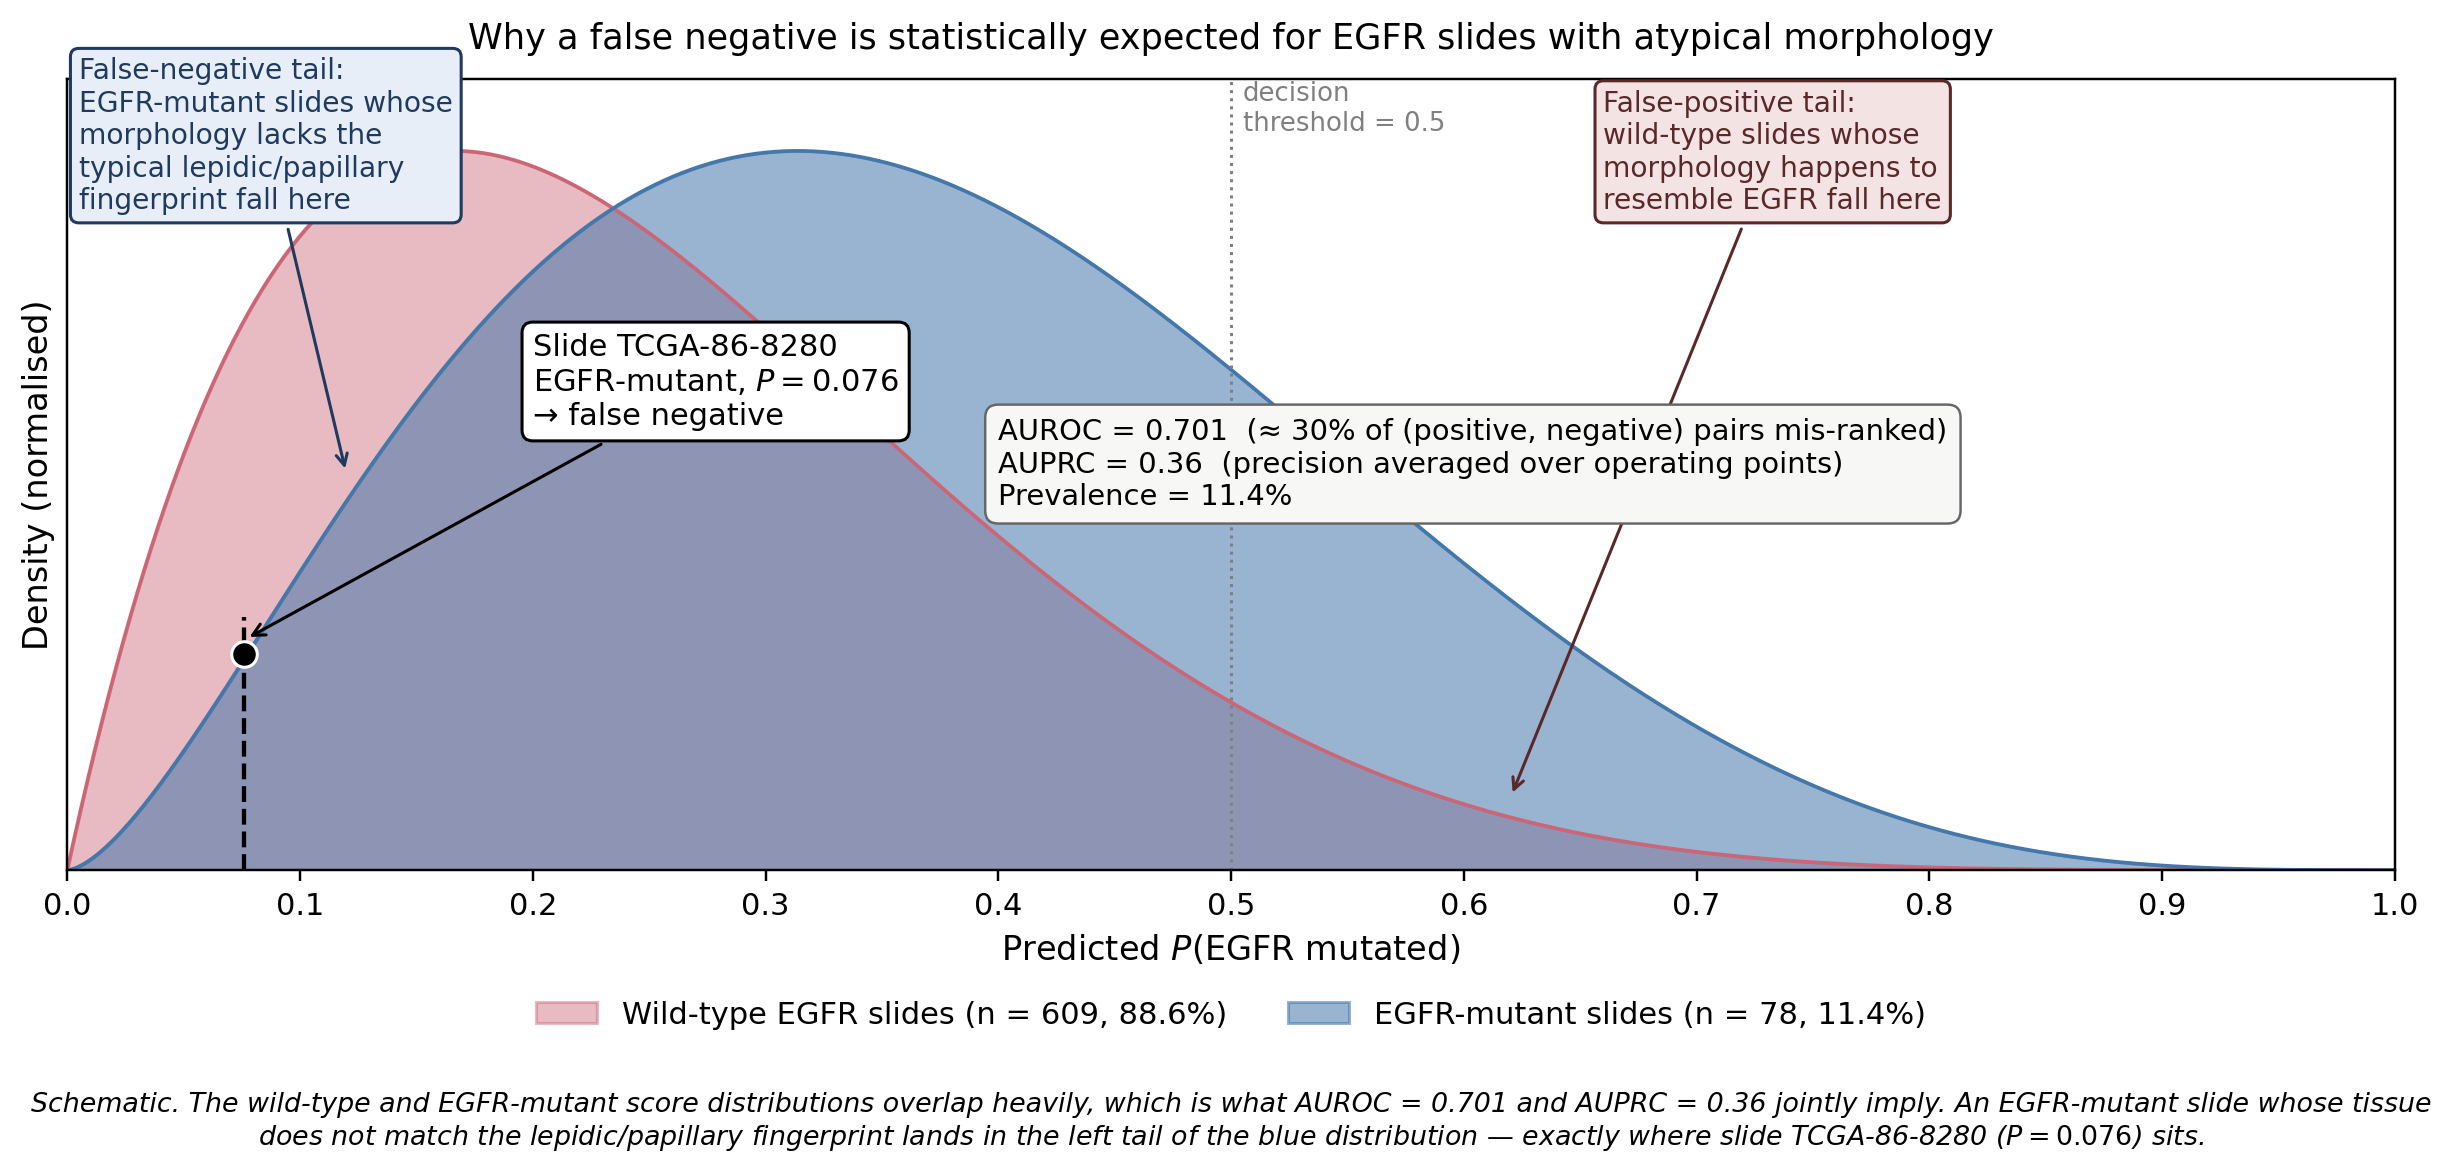
\includegraphics[width=\textwidth]{chapters/figures/egfr_score_overlap.png}
\caption[Why a false negative is statistically expected for atypical
EGFR cases]{%
    Schematic illustration of why slide TCGA-86-8280 ($P = 0.076$,
    EGFR-mutant) is a statistically expected false negative.
    The two density curves are illustrative score distributions for
    wild-type ($n = 609$, red) and EGFR-mutant ($n = 78$, blue)
    slides, calibrated so that their separation reproduces the
    reported AUROC $= 0.701$ on a comparable cohort.
    AUROC $= 0.701$ implies that around $30\%$ of (positive, negative)
    slide pairs are mis-ranked; AUPRC $= 0.36$ is a separate symptom
    of the same overlap, expressing the precision penalty at typical
    operating points (the false-positive side, right tail of the red
    curve).
    The same overlap also produces false negatives (left tail of the
    blue curve), where EGFR-mutant slides whose morphology lacks the
    typical lepidic/papillary fingerprint receive low predicted
    probabilities.
    TCGA-86-8280 sits at $P = 0.076$, well inside the false-negative
    tail.}
\label{fig:egfr_score_overlap}
\end{figure}

The ablation comparison confirms the absence of signal: all three
models (Combined 7.1\%, Emb-only 7.6\%, Pat-only 10.3\%) produce
near-zero probabilities, meaning that neither the visual texture
nor the pattern classification captures EGFR evidence on this
slide.

\paragraph{Per-slide model arbitration is moot on this slide.}
With every ablation pathway near zero, no counterfactual
rescue is available: the question \emph{``would another model
have predicted this slide correctly?''} resolves negatively
for every candidate, and the slide-level outcome coincides
with what the gene-level model selection rule would have
produced under any of the four available models.
This is the conservative behaviour the rule is designed to
deliver when the morphological signal is genuinely absent
rather than merely mismatched.
The same rule, on slides where one ablation \emph{does}
expose a counterfactual rescue (e.g.\ KEAP1 slide
TCGA-49-AAR9; Section~\ref{sec:eval:tcga:keap1}), forbids the
per-slide override; its formal justification is given in
Section~\ref{sec:meth:interp:gene_vs_slide_selection}
(Figure~\ref{fig:per_slide_arbitration_fails}).

\textbf{Why this failure is informative, not just wrong.}
This is the case for which the framework's three-channel
explanation surface earns its keep.
A clinician viewing the LCHAI output sees three pieces of
evidence simultaneously:
(i)~a very low EGFR probability ($P = 0.076$),
(ii)~the explicit absence of the EGFR-associated lepidic/%
papillary patterns in the overlay,
and (iii)~a \emph{Conclusive} cohort-level label indicating
that the model is, in expectation, reliable for EGFR.
That combination has a clear operational reading---the input
does not match the trained input distribution for the positive
class, so the low probability is consistent with a morphological
mismatch rather than a reliable wild-type call---and it prompts
a confirmatory molecular test.
Without the explanation surface, a clinician seeing only
``$P = 0.076$'' might treat the slide as wild-type and skip
testing; with it, the prediction is correctly read as
\emph{out-of-distribution-like} for this gene, not as a high-%
confidence negative.

\textbf{Keeping the pattern--mutation associations current.}
The reasoning above relies on the canonical association
EGFR~$\leftrightarrow$~lepidic/papillary
(Yoshizawa~et~al.~\cite{yoshizawa2013egfrmorph}), but the
literature on uncommon EGFR variants (exon~20 insertions, G719X,
S768I, L861Q) keeps evolving~\cite{brindel2020uncommonegfr}.
LCHAI~v2.0 does not freeze these associations into the model: they
are stored explicitly in the three-tier knowledge graph
(Section~\ref{sec:eval:rq6}), where every edge carries a
\texttt{provenance} attribute distinguishing curated assertions
(WHO, OncoKB, FDA) from inferred or discovered relations.
The DeepSearch pipeline (Section~\ref{sec:eval:rq7}) periodically
queries PubMed, Semantic Scholar, and arXiv and incorporates new
discovered relations as versioned additions on the next rebuild,
while contradicted edges (e.g., the acinar~$\to$~KRAS link
deactivated based on pooled evidence) can be retired without losing
the audit record.
For a case like TCGA-86-8280, this means the explanation surface
will reflect the current evidence base on EGFR variant morphology
even if the underlying CNN remains unchanged---decoupling what the
system \emph{believes about the literature} from what the model
\emph{has been trained on}.


\subsubsection{KRAS: Micropapillary-Classified Predominant Tumour with High
FC-MIL Prediction}
\label{sec:eval:tcga:kras}

Figure~\ref{fig:attn_kras_tp} shows the LCHAI~v2.0 output for slide
TCGA-55-7815, a KRAS-mutant case predicted with very high confidence
via FC-MIL (P(mut)~$= 0.965$, method: FC-MIL).
KRAS carries a population-level \textbf{Inconclusive} label regardless
of this slide-level confidence (cohort mean 5-fold
AUROC~$= 0.609 < 0.70$; Table~\ref{tab:viz_folds})---the system
caveats the prediction at the gene-cohort level even when the
per-slide confidence is high, which is the precise behaviour the
Conclusive/Inconclusive criterion is designed to enforce.
The slide is 79.44\% micropapillary-classified with 17.14\% acinar content and minor
cribriform (2.5\%) and solid (0.64\%) components.
The SHAP balance is 59\% embedding / 41\% pattern (fuzzy
classification: \emph{Balanced}).

\emph{Model-level parameters, slide-level inputs.}
The 21 parameters of the 2-additive fuzzy measure $\mu$ (the six
Shapley values $\phi_k$ plus the fifteen pairwise interaction
indices $I_{kl}$;
Equation~\ref{eq:fuzzy_measure_method},
Section~\ref{sec:meth:choquet:params}) are learned during training
and frozen in the deterministic checkpoint (\texttt{seed=42}).
We therefore call them \emph{global} in the sense of
\emph{model-level rather than case-level}: the same 21 numbers
govern the Choquet aggregation for every KRAS slide, every TP53
slide, and so on---they characterise what FC-MIL learned, not this
particular case.
What changes from slide to slide are the pattern memberships
$\mathbf{p}_i$ over which those weights are aggregated; we report
$\phi_k$ and $I_{kl}$ on TCGA-55-7815 only to make their effect
concrete on a real slide.

\emph{Where the FC-MIL signal actually lives.}
The Shapley values ($\phi_{\text{cri}} = 0.170$,
$\phi_{\text{sol}} = 0.168$, $\phi_{\text{aci}} = 0.167$;
Table~\ref{tab:choquet_shapley}) are essentially flat---all six
channels sit within $\pm 0.005$ of the uniform value $1/6 \approx
0.167$ and are classified as \emph{Near-Uniform}.
A near-uniform Shapley profile means the model has no preferred
single pattern for KRAS; on its own, this profile is not
discriminative.
The genuine FC-MIL contribution on KRAS lies in the
\emph{interaction indices}: lepidic$\times$solid
($I = +0.032$; \emph{Moderate Synergy}) and solid$\times$acinar
($I = +0.025$;
Table~\ref{tab:choquet_interactions}).
These positive $I_{kl}$ tell the Choquet aggregator that
\emph{co-occurrences} of these pattern pairs within a slide are
more informative than either pattern individually---which is the
mechanism standard additive heads cannot capture.

\begin{figure}[ht!]
\centering
\begin{minipage}[t]{0.48\textwidth}
\centering
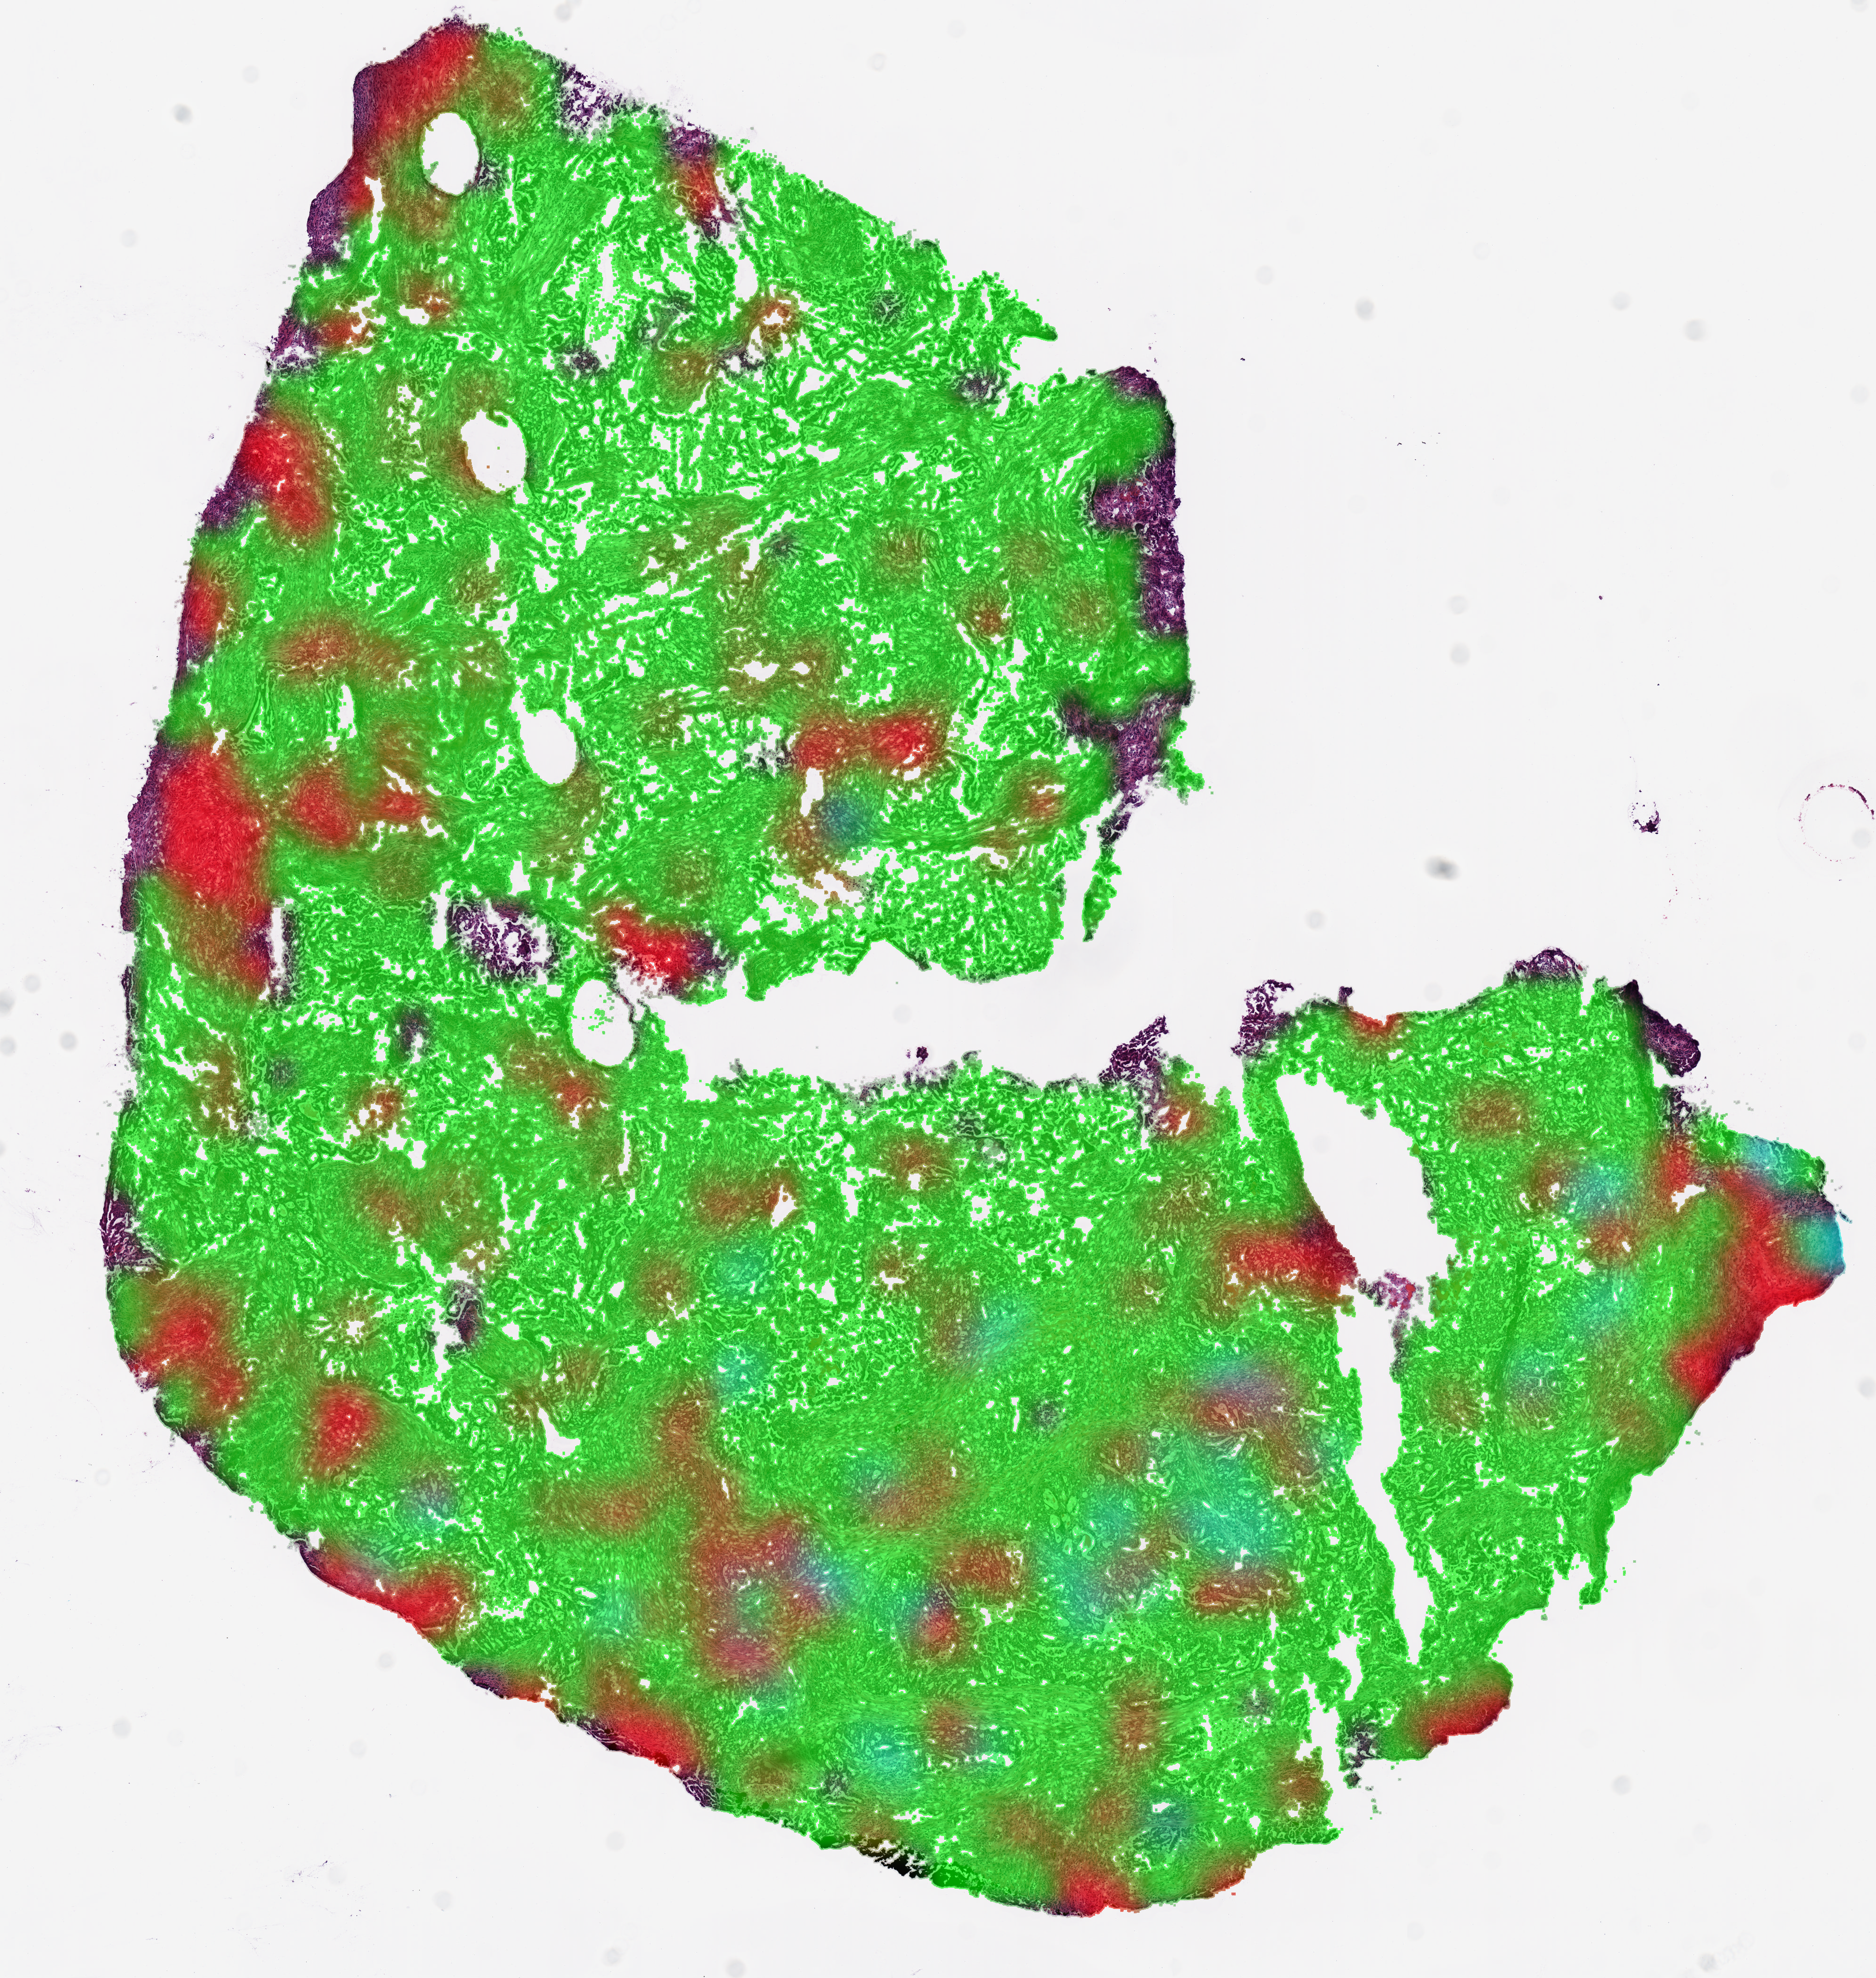
\includegraphics[width=\textwidth]{chapters/figures/lchai_v2_KRAS_TCGA-55-7815_pattern_overlay.png}
\end{minipage}\hfill
\begin{minipage}[t]{0.48\textwidth}
\centering
\includegraphics[width=\textwidth]{chapters/figures/lchai_v2_KRAS_TCGA-55-7815_attention_map.png}
\end{minipage}\\[6pt]
\begin{minipage}[t]{0.48\textwidth}
\centering
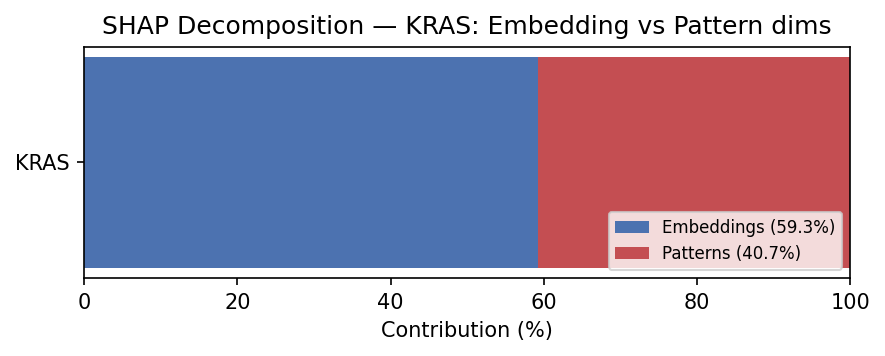
\includegraphics[width=\textwidth]{chapters/figures/shap_decomp_KRAS_55_7815_bar.png}
\end{minipage}\hfill
\begin{minipage}[t]{0.48\textwidth}
\centering
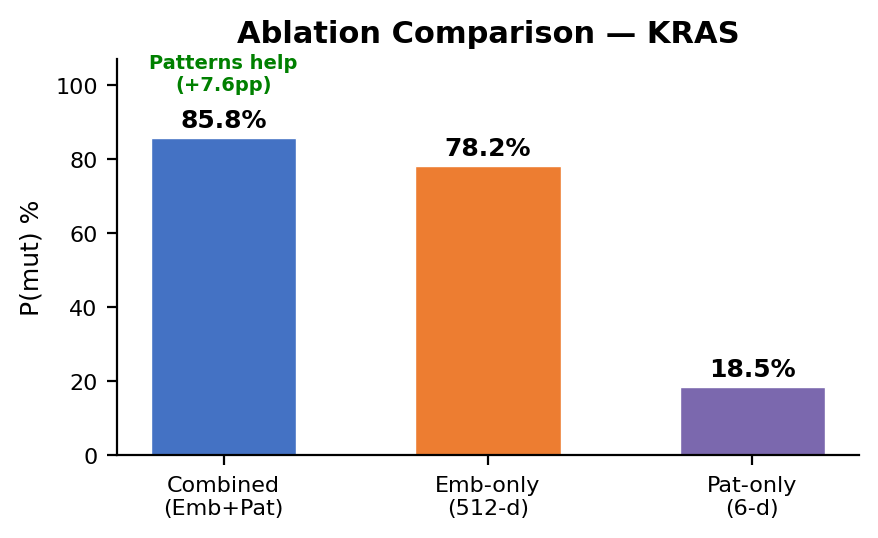
\includegraphics[width=\textwidth]{chapters/figures/ablation_KRAS_55_7815.png}
\end{minipage}
\caption[LCHAI~v2.0 interpretability: KRAS (TCGA-55-7815)]{%
    LCHAI~v2.0 interpretability for KRAS-mutant slide TCGA-55-7815
    (P(mut)~$= 0.965$, FC-MIL; population-level: Inconclusive).
    \textbf{Top left}: Pattern overlay---micropapillary-dominant (79.44\%, green)
    with acinar clusters (17.14\%, red).
    \textbf{Top right}: ABMIL attention map.
    \textbf{Bottom left}: SHAP decomposition---59\% embedding / 41\% pattern.
    \textbf{Bottom right}: Ablation---Combined (85.8\%) outperforms Emb-only
    (78.2\%), the \emph{only gene where patterns measurably improve prediction}
    ($+7.6$\,pp).}
\label{fig:attn_kras_tp}
\end{figure}

\textbf{Interpretation.}
KRAS mutations are clinically associated with solid tumour areas
and with a LUAD subtype called
\emph{invasive mucinous adenocarcinoma} (IMA), in which tumour
cells secrete abundant mucus and grow along the existing
alveolar walls---visually, IMA mixes lepidic-like and solid-like
tile appearances on the slide~\cite{shim2015krasmucinous}.
The challenge for the system is a label-space gap: the ANORAK
output ontology used by the pattern channel has \emph{no
dedicated IMA class}, so IMA cannot be expressed as a single
canonical $\mathbf{e}_k$ basis vector in the 6-d pattern simplex.
Yet the model returns $P(\text{mut}) = 0.965$ on this slide---a
high-confidence true positive.
The puzzle is resolved by Finding~2
(Section~\ref{sec:eval:mutation:finding2};
Figure~\ref{fig:kras_lepidic_solid_proxy}): FC-MIL learns to
\emph{re-encode} IMA as a lepidic--solid co-presence---i.e.\ a
non-canonical \emph{interaction term} on the pattern simplex
rather than a coordinate axis---which is exactly what the
$I_{\,\mathrm{lepidic,\,solid}} = +0.032$ index quantifies.
Two slide-level remarks complement that broader explanation.

\emph{Scale of the interaction index.}
Although $I = +0.032$ may appear small in absolute terms, this is
the expected scale for interaction indices under the $L_1$
regulariser ($\lambda_I = 0.01$,
Equation~\ref{eq:interaction_reg}): the regulariser penalises large
interactions to prevent overfitting, so surviving non-zero values
represent genuine learned structure rather than noise.

\emph{What the index does mechanically.}
The interaction index does not directly add $3.2$ percentage points
to $P(\text{mut})$; it modifies the fuzzy measure so that subsets
containing \emph{both} lepidic and solid receive higher measure
values, altering the Choquet aggregation of pattern scores before
the classification head produces the final probability.
Figure~\ref{fig:kras_mu_subset_lattice} makes this concrete on
TCGA-55-7815: of the four relevant subsets of
$\{\mathrm{lepidic},\,\mathrm{solid}\}$, only one---the joint
subset---receives a bump, raising
$\mu(\{\mathrm{lep,\,sol}\})$ from $0.333$ (the additive baseline
$\phi_{\mathrm{lep}} + \phi_{\mathrm{sol}}$) to $0.365$.

\begin{figure}[!htbp]
\centering
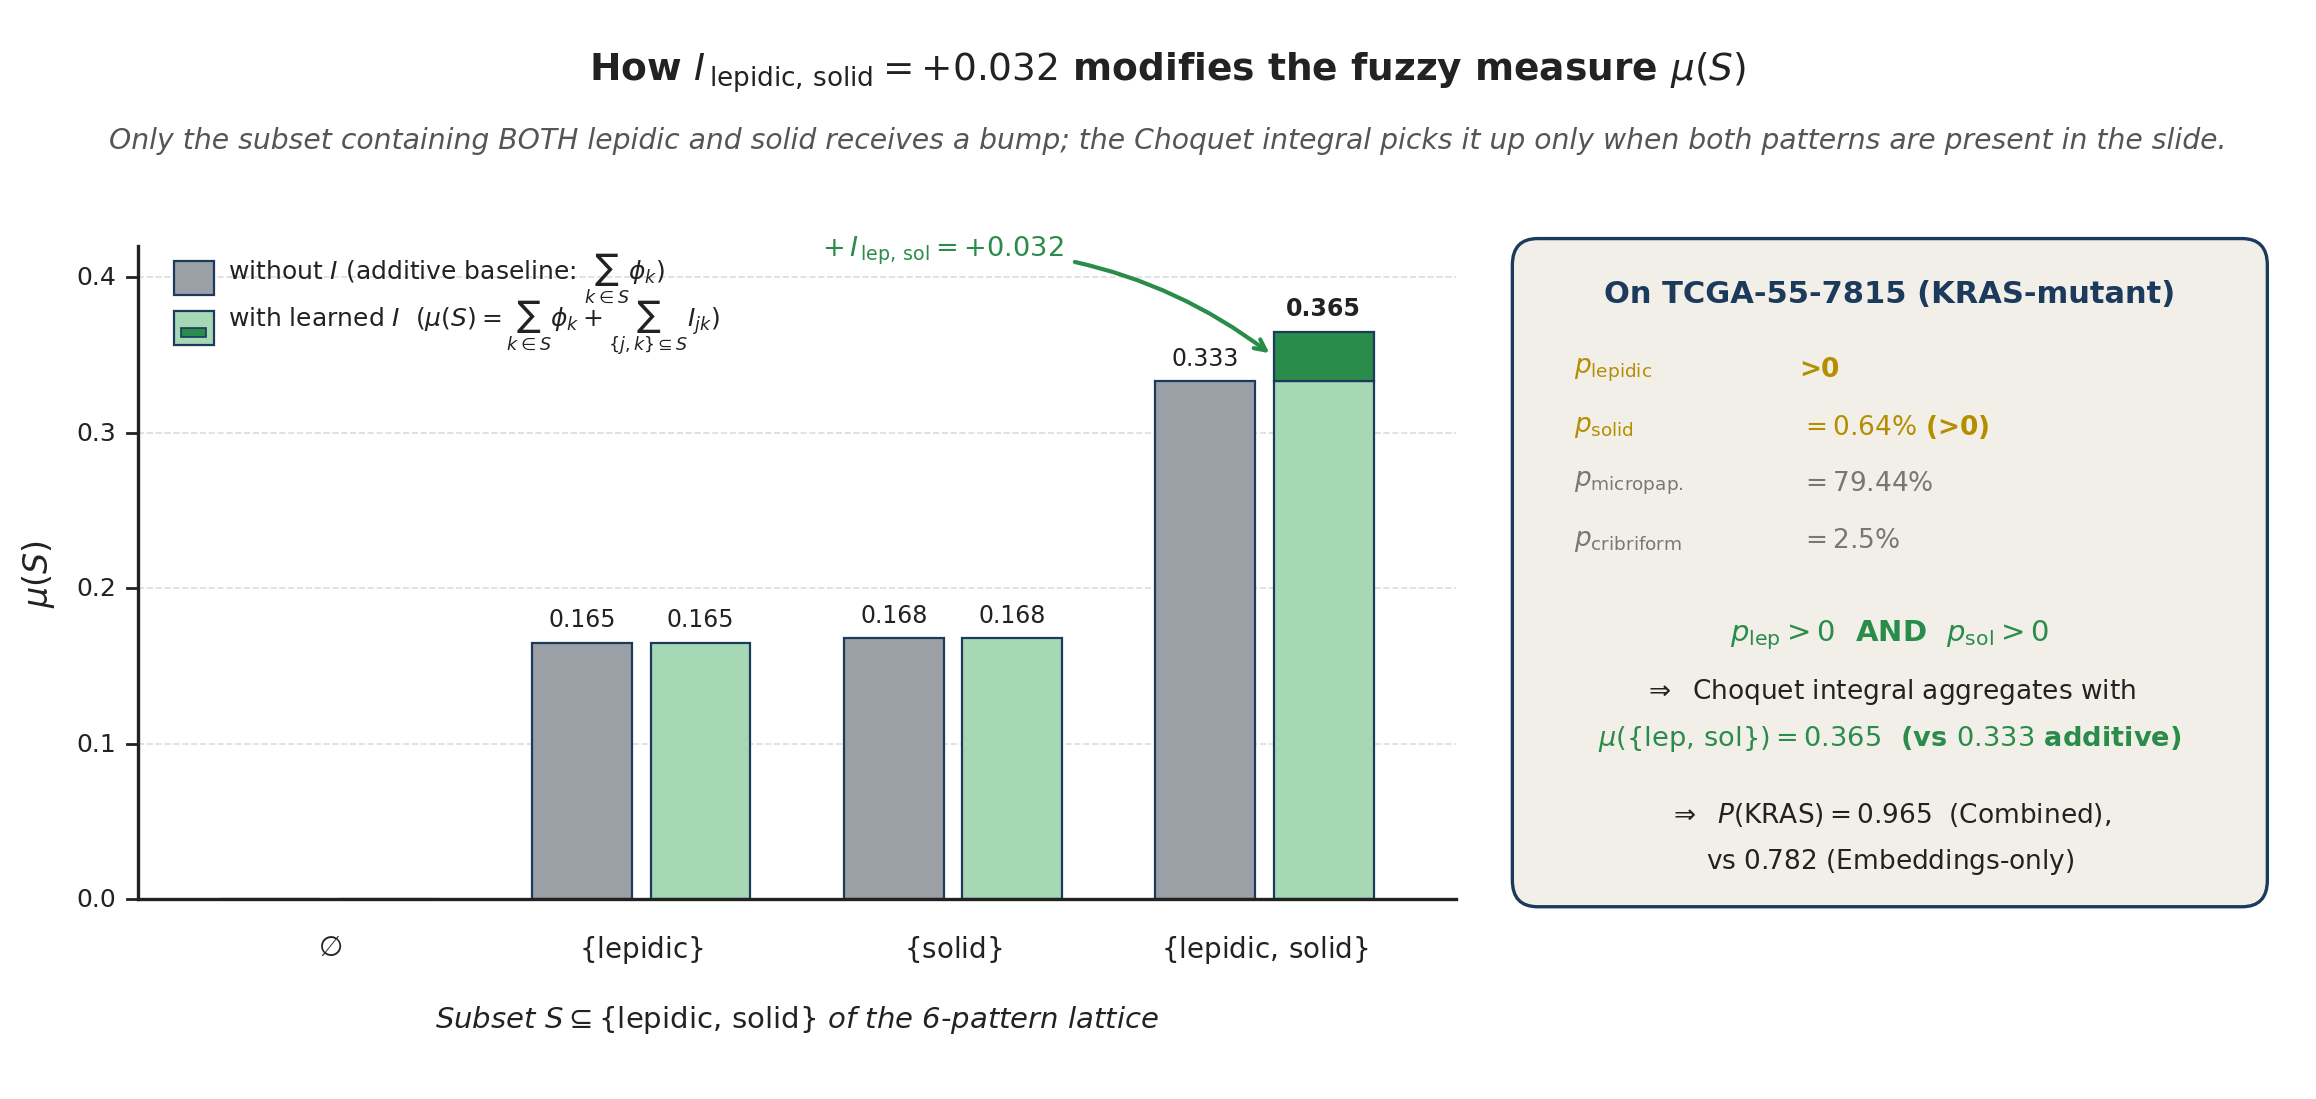
\includegraphics[width=\textwidth]{chapters/figures/kras_mu_subset_lattice.png}
\caption[How $I_{\,\mathrm{lep,\,sol}}$ modifies $\mu(S)$ on
TCGA-55-7815]{%
    Mechanistic effect of $I_{\,\mathrm{lepidic,\,solid}} = +0.032$
    on $\mu(S)$ for KRAS, on the four subsets
    $S \subseteq \{\mathrm{lepidic},\,\mathrm{solid}\}$
    ($\phi_{\mathrm{lep}} = 0.165$, $\phi_{\mathrm{sol}} = 0.168$;
    Table~\ref{tab:choquet_shapley}).
    Only $\mu(\{\mathrm{lep,\,sol}\})$ rises (from $0.333$ to
    $0.365$): the other three subsets are unchanged because the
    interaction term only fires when \emph{both} patterns are in
    $S$.
    Right panel: on TCGA-55-7815 both memberships are non-zero, so
    the Choquet integral uses the bumped value, contributing to the
    $+7.6$\,pp Combined-vs-Embeddings gap reported in
    Figure~\ref{fig:attn_kras_tp}.}
\label{fig:kras_mu_subset_lattice}
\end{figure}

\emph{Ablation confirmation on this slide.}
The Combined model (85.8\%) outperforms the Embeddings-only model
(78.2\%) by $+7.6$\,pp (ablation panel in
Figure~\ref{fig:attn_kras_tp}).
\textbf{KRAS is the only gene among the six where adding pattern
information measurably improves the prediction}, in line with its
classification under regime~C (\emph{constructive}) of Finding~6
(Section~\ref{sec:eval:mutation:finding6})---the only gene in
the cohort where the Choquet branch operates as an active
discriminative module.


\subsubsection{STK11: Low Prediction in a Micropapillary-Classified Dominant Slide}
\label{sec:eval:tcga:stk11}

Figure~\ref{fig:attn_stk11_tp} shows the LCHAI~v2.0 output for slide
TCGA-49-AAR0, an STK11-mutant case predicted with low mutation
probability (P(mut)~$= 0.046$, method: PI-ABMIL;
population-level: \textbf{Inconclusive}, cohort mean 5-fold
AUROC~$= 0.695 < 0.70$; Table~\ref{tab:viz_folds}).
As established in the case-study preamble
(Section~\ref{sec:eval:interp:attention}), the slide-level
evidence below does \emph{not} re-label this slide; it explains
\emph{why} the cohort AUROC sits where it does.
The slide is overwhelmingly micropapillary-classified ($98.68\%$)
with negligible representation of other patterns (acinar
$0.89\%$, solid $0.41\%$).
The SHAP decomposition shows $90\%$ embedding / $10\%$ pattern
contribution (fuzzy classification: \emph{Embedding-Dominated}).

At the population level, STK11 sits in regime~B
(\emph{engaged-but-unproductive}) of Finding~6
(Section~\ref{sec:eval:mutation:finding6}): the Choquet branch
trains over a feature space that carries no STK11-discriminative
signal because the actual signal lives in the tumour
microenvironment---outside the ANORAK simplex---which is the
\emph{label-space mismatch} mechanism of the
ontology-coverage taxonomy
(RQ2(ii); Figure~\ref{fig:signal_tree}).
FC-MIL underperforms B2 by $-0.026$ AUROC
($0.658$ vs $0.684$; Table~\ref{tab:mutation_luad}), B2 lifts the
prediction with the sole help of CTransPath embeddings, and
PI-ABMIL leads marginally at AUROC~$0.695$ ($+0.011$ vs B2;
Table~\ref{tab:p_vs_b2})---a sub-significant cohort tie within
fold variance ($d \approx 1.2$ MDE; Section~\ref{sec:eval:limitations})
that the per-slide ablation contradicts
($\Delta_{\mathrm{pat}} = -5.5$\,pp;
Table~\ref{tab:enrichment_summary}).
The engagement map of Figure~\ref{fig:choquet_variance_map}
(upper-left, \emph{engagement without conversion}) refines this
picture: the Choquet branch activates fold-specifically
($\Delta\sigma = +0.035$) but never converges on a discriminative
pattern subset---each fold's training set offers a different
spurious correlate, the optimiser explores them, none generalises.
The slide-level evidence below makes the same diagnosis concrete
on a single representative case.

\begin{figure}[ht!]
\centering
\begin{minipage}[t]{0.48\textwidth}
\centering
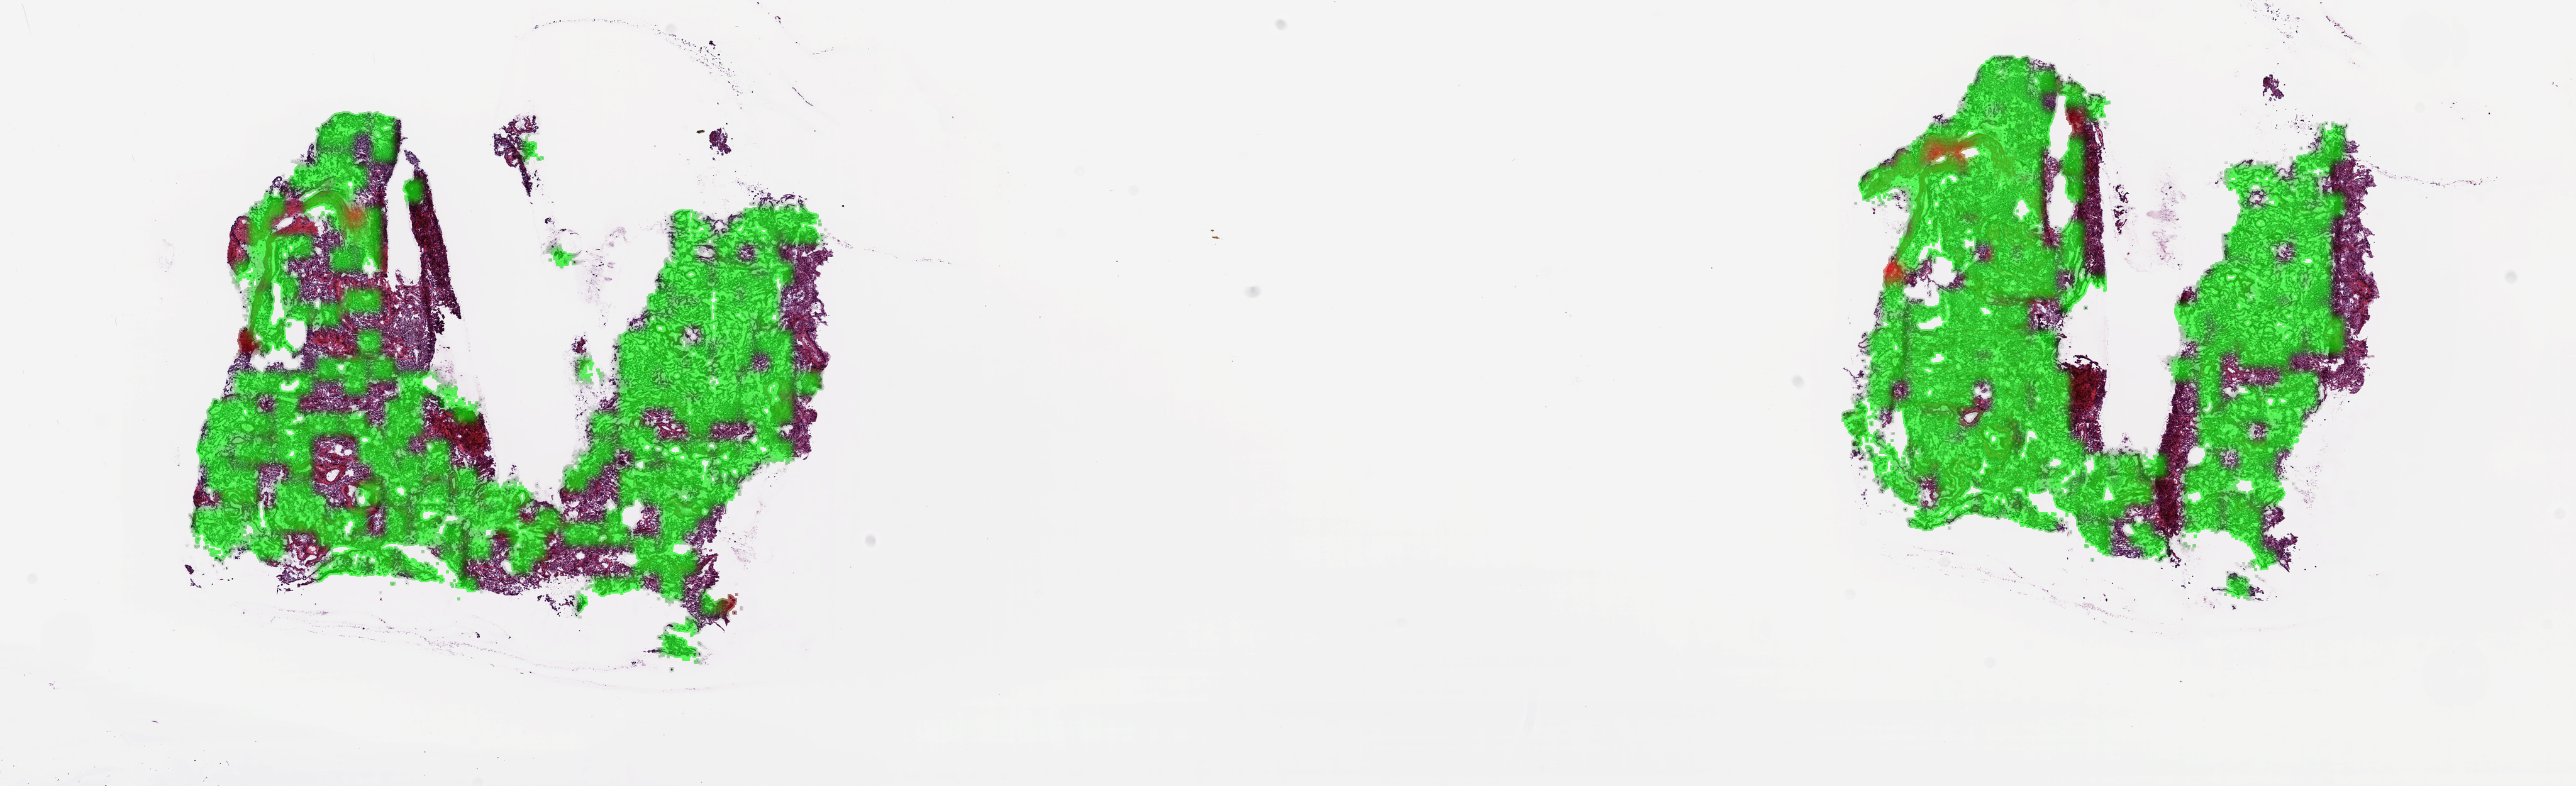
\includegraphics[width=\textwidth]{chapters/figures/lchai_v2_STK11_TCGA-49-AAR0_pattern_overlay.png}
\end{minipage}\hfill
\begin{minipage}[t]{0.48\textwidth}
\centering
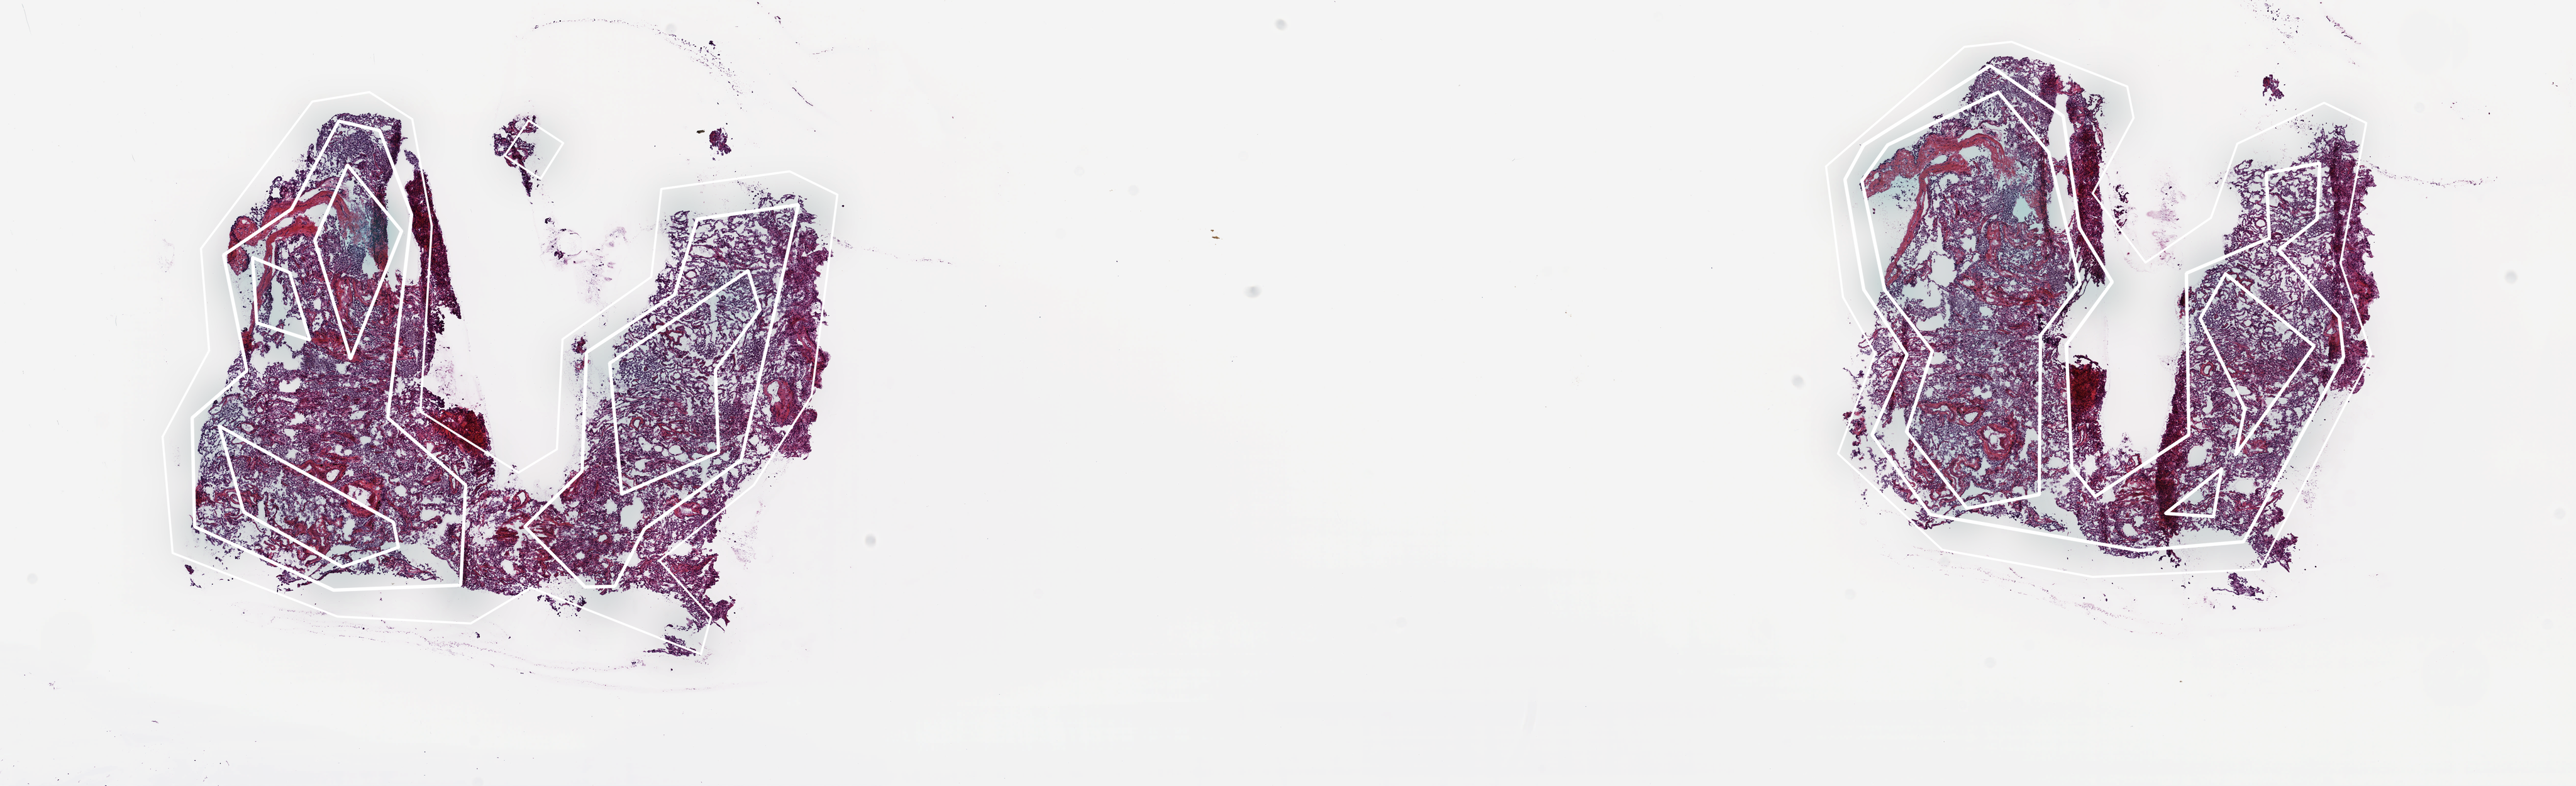
\includegraphics[width=\textwidth]{chapters/figures/lchai_v2_STK11_TCGA-49-AAR0_attention_map.png}
\end{minipage}\\[6pt]
\begin{minipage}[t]{0.48\textwidth}
\centering
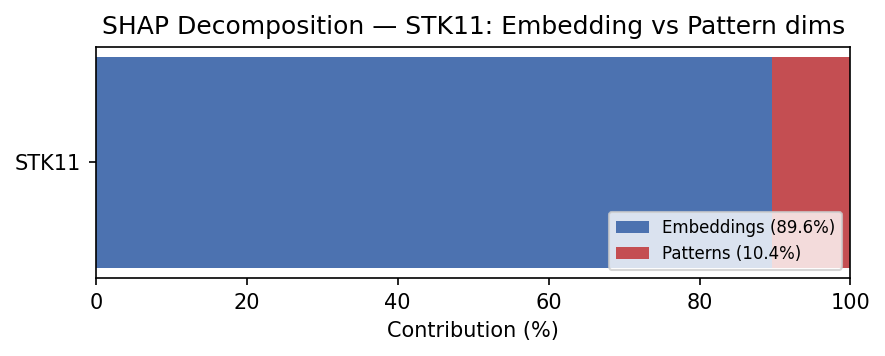
\includegraphics[width=\textwidth]{chapters/figures/shap_decomp_STK11_49_AAR0_bar.png}
\end{minipage}\hfill
\begin{minipage}[t]{0.48\textwidth}
\centering
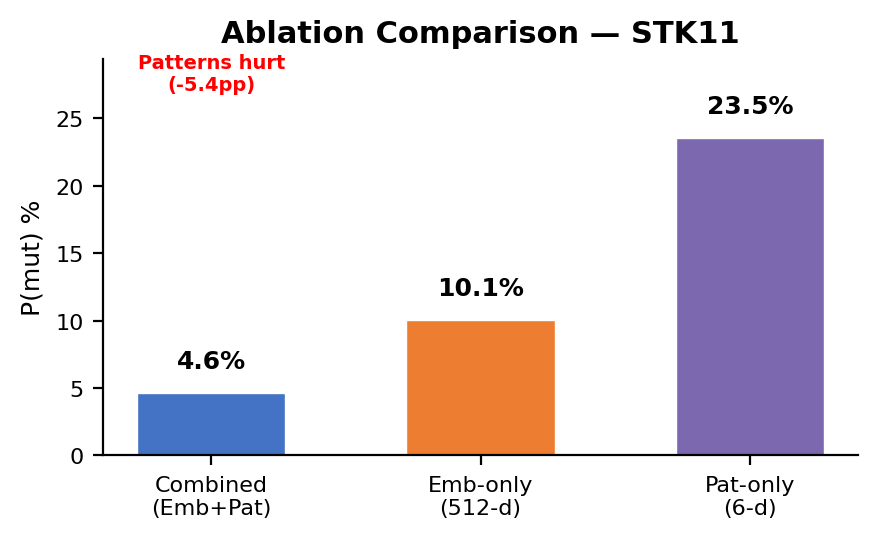
\includegraphics[width=\textwidth]{chapters/figures/ablation_STK11_49_AAR0.png}
\end{minipage}
\caption[LCHAI~v2.0 interpretability: STK11 (TCGA-49-AAR0)]{%
    LCHAI~v2.0 interpretability for STK11-mutant slide TCGA-49-AAR0
    (P(mut)~$= 0.046$, PI-ABMIL; population-level: Inconclusive).
    \textbf{Top left}: Pattern overlay---near-homogeneous micropapillary (98.68\%).
    \textbf{Top right}: ABMIL attention map---sparse and diffuse.
    \textbf{Bottom left}: SHAP decomposition---90\% embedding / 10\% pattern.
    \textbf{Bottom right}: Ablation---Combined (4.6\%) $<$ Emb-only (10.1\%):
    patterns degrade prediction on this homogeneous slide.}
\label{fig:attn_stk11_tp}
\end{figure}

\textbf{Interpretation.}
STK11 illustrates a \emph{label-space mismatch}: the gene's
discriminative signal lives outside the feature space the
pattern channel was designed to represent.
At the architectural scale STK11 mutations do not produce a
discriminative growth-pattern fingerprint: although
STK11-mutant tumours are over-represented in aggressive
\emph{Grade~3 morphologies}---the most disordered, fastest-%
growing tissue layouts under the standard LUAD grading scheme,
predominantly solid and, to a lesser extent,
micropapillary~\cite{pineda2025stk11morphology}---those same
patterns are also frequent in TP53- and KRAS-mutant tumours,
so the marginal distribution over the ANORAK pattern simplex
is approximately invariant across STK11 status and the
pattern channel cannot disambiguate STK11 from other drivers.
The distinctive STK11 signal lives instead in the
\emph{tumour microenvironment} (TME, the non-tumour cellular
context surrounding the tumour, including immune cells and
supporting stroma).
STK11 inactivation depletes
\emph{tumour-infiltrating lymphocytes} (TILs, the immune cells
that normally enter a tumour and attack
it) and produces an \emph{immune-cold} phenotype---a tumour
with very few infiltrating immune
cells~\cite{skoulidis2015krassubsets,skoulidis2018stk11pd1}.
This is the channel where the STK11 signal actually lives;
crucially, it is not represented as an output class in the
six-pattern ANORAK ontology used by the pattern channel,
because ANORAK was trained to recognise tumour growth
architecture, not microenvironmental composition.
Whatever STK11 evidence the system can recover must therefore
be encoded inside the CTransPath embeddings as latent texture,
without an explicit symbolic anchor.
DNA sequencing confirms the STK11 mutation on this slide, yet
the model returns only $P(\text{mut}) = 0.046$---a
\textbf{false negative}.
Three factors explain why:

\begin{enumerate}
    \item \textbf{Documented but non-discriminative
    growth-pattern correlate.}
    Unlike EGFR (Section~\ref{sec:eval:tcga:egfr}, where
    lepidic and papillary patterns are \emph{specifically}
    associated with the mutation but are simply absent on the
    EGFR false-negative slide), the histological signature of
    STK11 is documented but
    non-specific: Pineda et~al.~\cite{pineda2025stk11morphology}
    report that STK11-mutant LUADs cluster in aggressive
    Grade~3 morphologies---predominantly solid, and to a lesser
    extent micropapillary---but these same patterns are equally
    enriched in TP53- and KRAS-mutant tumours, so the pattern
    channel cannot use them to disambiguate STK11 from other
    drivers.
    The slide TCGA-49-AAR0 is, in fact,
    $98.68\%$ micropapillary, exactly within the morphology
    spectrum reported by Pineda et~al., yet on its own that
    pattern is uninformative for the gene-level call.
    The complementary STK11 signal---an immune-cold tumour
    microenvironment with reduced
    TILs~\cite{skoulidis2015krassubsets,skoulidis2018stk11pd1}---falls
    outside the six-pattern ANORAK ontology entirely.
    Whatever STK11 signal the system recovers must therefore
    live in the CTransPath embeddings, which is exactly the
    biology behind STK11's embedding-dominant classification at
    the population level
    (Finding~6, Section~\ref{sec:eval:mutation:finding6};
    Figure~\ref{fig:choquet_regimes}, right).
    Like KEAP1 (Section~\ref{sec:eval:tcga:keap1}) and RBM10
    (the next case study), STK11 is a gene whose
    \emph{discriminative} effect is biological-but-not-%
    morphological in the ANORAK sense.

    \item \textbf{The pattern channel is actively
    counterproductive on this slide ($-5.5$\,pp).}
    The slide is morphologically near-homogeneous
    ($98.68\%$ micropapillary), so the 6-d pattern vector is
    nearly one-hot.
    The ablation panel of Figure~\ref{fig:attn_stk11_tp} shows
    the consequence: the Embeddings-only model reaches
    $10.1\%$, whereas the Combined model drops to $4.6\%$, a
    $-5.5$\,pp pattern penalty.
    Both probabilities sit \emph{below} the $0.5$ decision
    threshold and the slide remains a false negative under
    either choice---unlike KEAP1, where the pattern penalty
    flipped a true positive into a false negative
    (Section~\ref{sec:eval:tcga:keap1}).
    The mechanism is the slide-level realisation of STK11's
    population-level \emph{engagement without conversion}
    signature
    (Figure~\ref{fig:choquet_variance_map}, upper-left): with
    no superadditive pattern pair to exploit, an active Choquet
    branch can only contribute variance, and on a near one-hot
    pattern vector that variance reduces to noise.

    \item \textbf{STK11 is population-level Inconclusive, with
    low prevalence and substantial AUROC--AUPRC gap.}
    STK11 has a cohort prevalence of $9.9\%$ (the
    second-lowest of the six target genes; $68$ mutated slides)
    and a mean 5-fold AUROC of $0.695$, which is \emph{below}
    the Hosmer--Lemeshow $0.70$ threshold for acceptable
    discrimination~\cite{hosmer2000applied} and earns STK11 the
    \emph{Inconclusive} label.
    Mechanically, AUROC~$= 0.695$ means roughly $30\%$ of
    (mutant, wild-type) pairs are mis-ranked, and the low
    prevalence forces precision down further: the corresponding
    mean AUPRC is only $\approx 0.31$
    (Figure~\ref{fig:auprc_by_gene}).
    This overlap manifests in both directions---wild-type
    slides receiving high STK11 scores (the false-positive
    side) and STK11-mutant slides receiving low scores (the
    false-negative side).
    A slide whose visual content lacks the specific
    micro\-en\-vi\-ron\-mental texture that CTransPath
    associates with STK11 is precisely the kind of case that
    falls into the low-score positive tail; on TCGA-49-AAR0
    that expectation materialises at $P = 0.046$.
\end{enumerate}

The clinical value of the framework here is that the system
communicates this caveat \emph{before} the prediction is even
viewed---the population-level Inconclusive label warns that the
model cannot reliably detect STK11 from tissue images alone and
that molecular testing is therefore required.
Figure~\ref{fig:stk11_signal_routes} consolidates the argument:
STK11 biology splits into two routes, one captured weakly by
the embedding pathway (\emph{partial},
Emb-only~$= 10.1\%$) and one closed in the pattern pathway
(\emph{closed}, Combined~$= 4.6\%$), and these are the
slide-level signatures of the cohort behaviour that earned the
gene its Inconclusive label.

\begin{figure}[ht!]
\centering
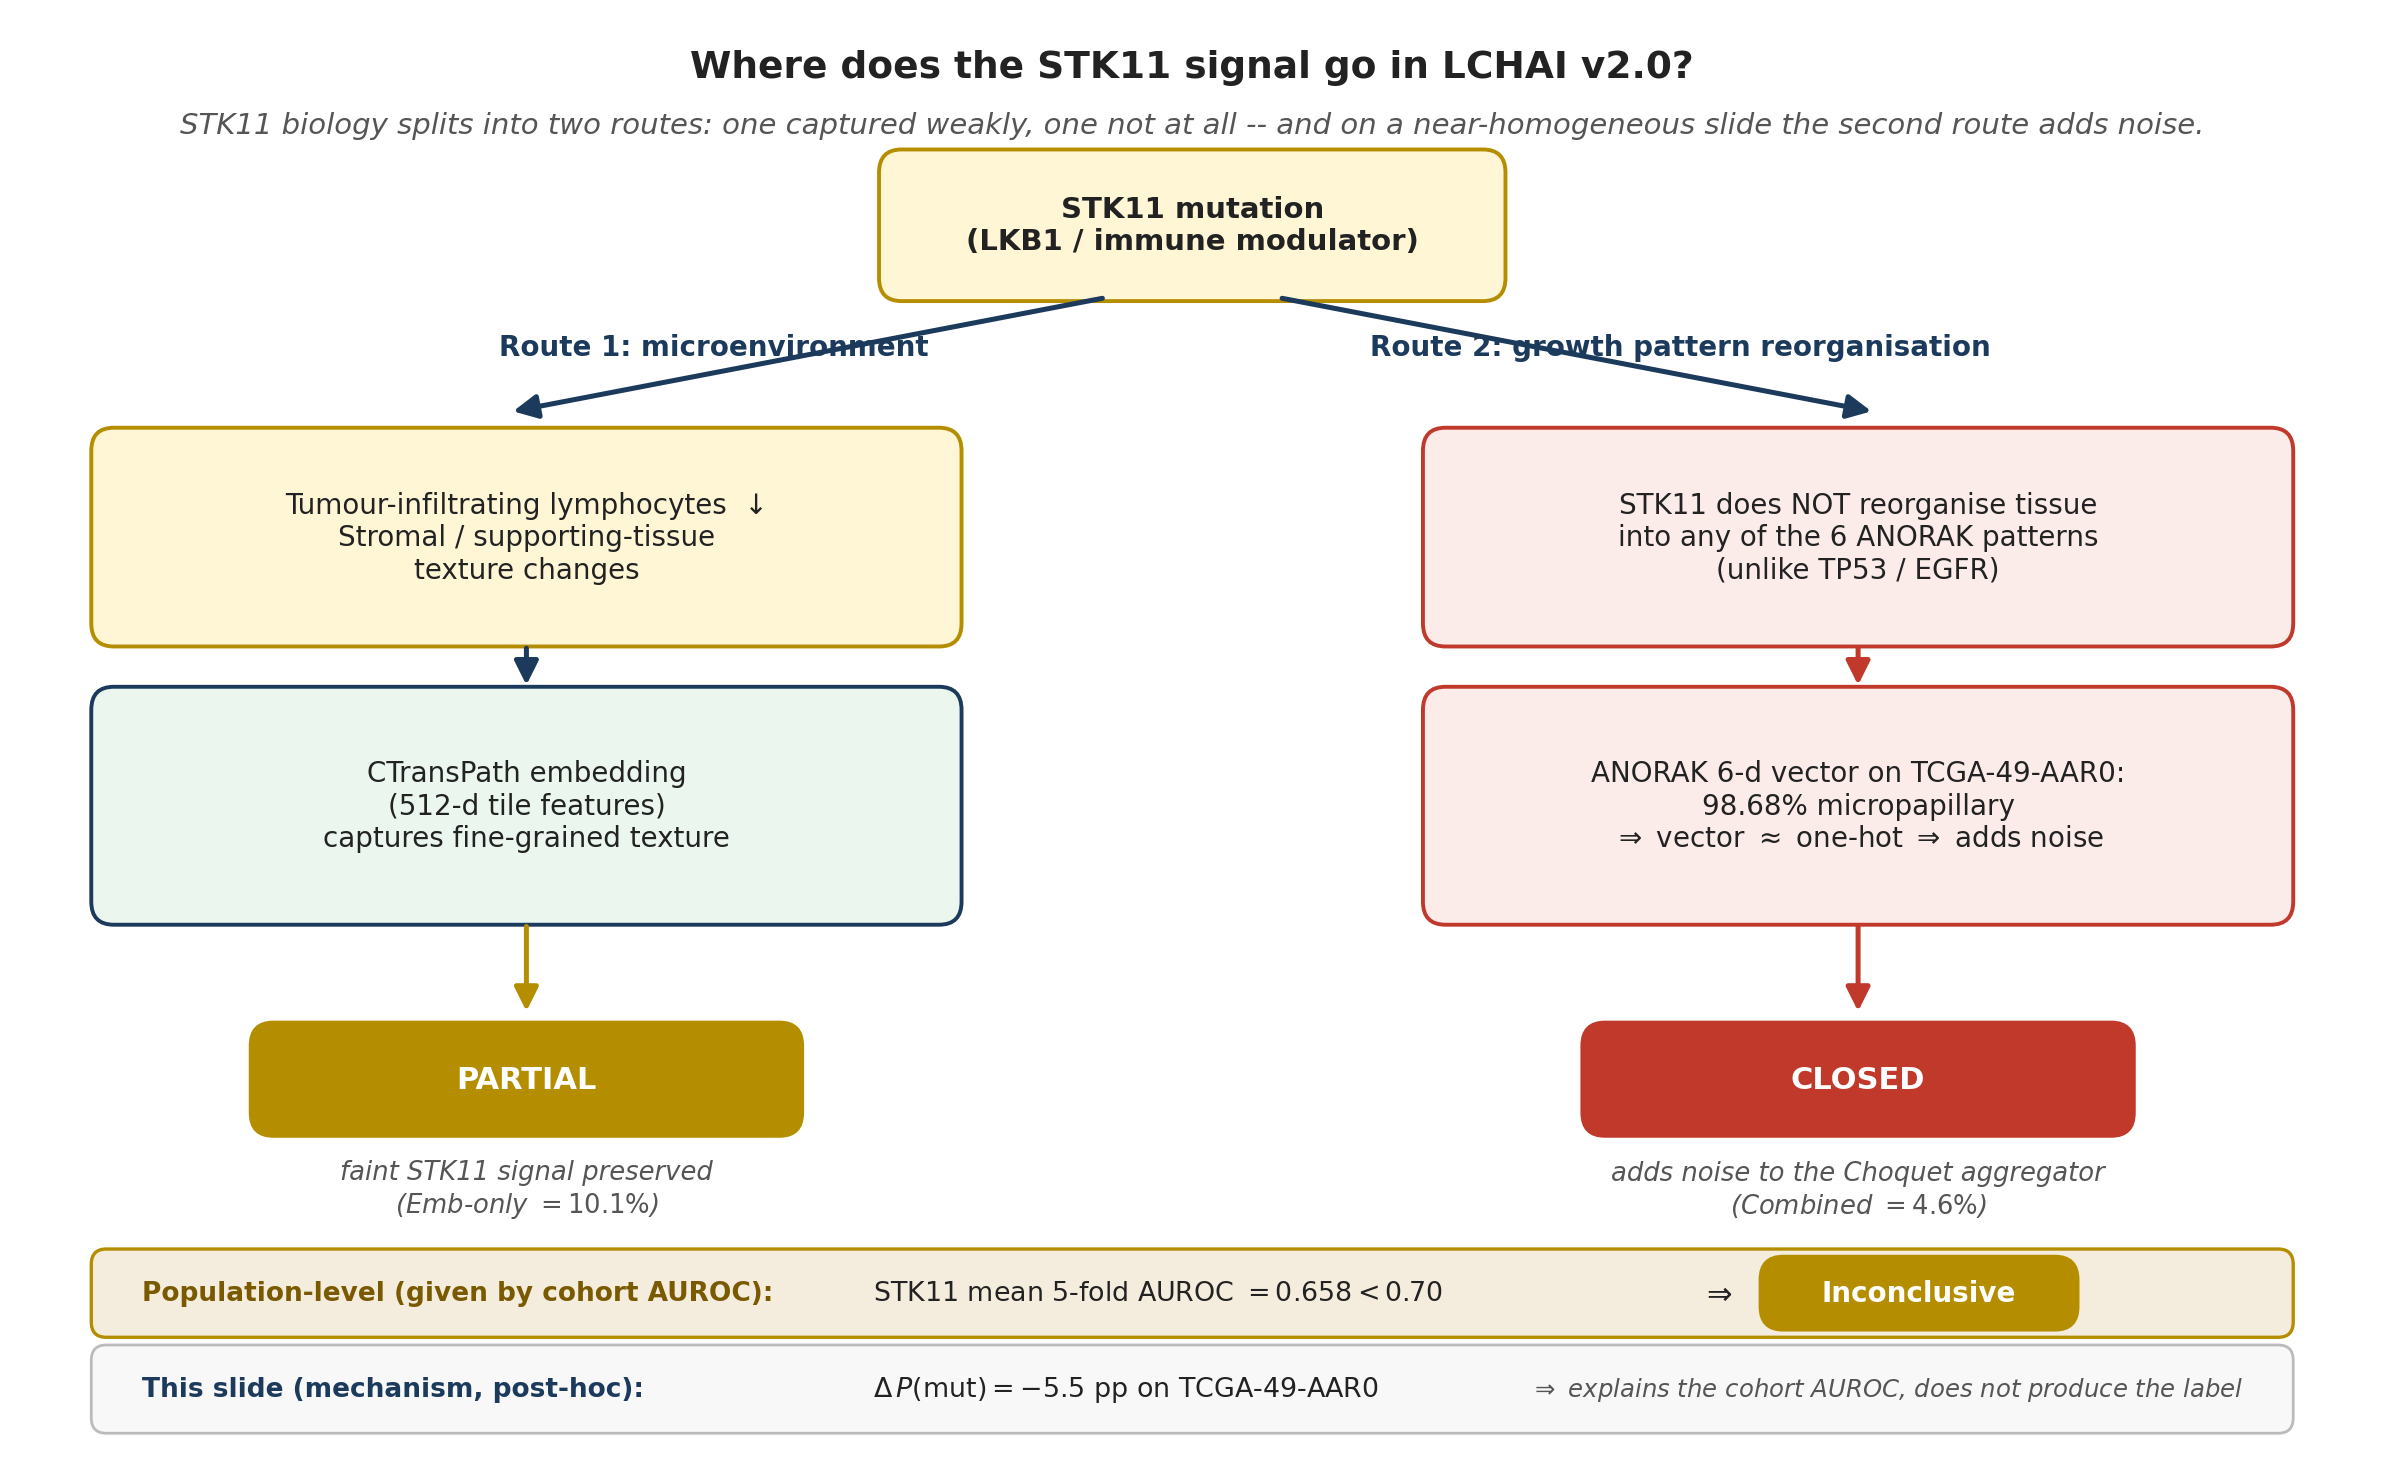
\includegraphics[width=\textwidth]{chapters/figures/stk11_signal_routes.png}
\caption[Where does the STK11 signal go in LCHAI~v2.0?]{%
    Two routes by which STK11 biology reaches the LCHAI~v2.0
    classifier on slide TCGA-49-AAR0.
    \textbf{Left} (microenvironment): STK11 produces an
    immune-cold tumour microenvironment with reduced
    TILs~\cite{skoulidis2015krassubsets,skoulidis2018stk11pd1};
    this signal falls outside the ANORAK growth-pattern
    ontology, and the CTransPath embedding captures it only
    weakly (\emph{partial}, Emb-only~$= 10.1\%$).
    \textbf{Right} (growth pattern): although STK11 is enriched
    in aggressive solid/micropapillary
    morphologies~\cite{pineda2025stk11morphology}, this
    association is non-discriminative against TP53- and
    KRAS-mutant tumours; on this
    $98.68\%$-micropapillary slide the 6-d pattern vector is
    near one-hot, so the Choquet branch only adds noise
    (\emph{closed}, Combined~$= 4.6\%$).
    Bottom bands separate the two levels of the conclusion---%
    \emph{given} (cohort AUROC $= 0.695 < 0.70$,
    population-level Inconclusive) and
    \emph{mechanism} ($\Delta P(\text{mut}) = -5.5$\,pp on this
    slide).
    See main text for the full reading.}
\label{fig:stk11_signal_routes}
\end{figure}

\paragraph{Why LCHAI~v2.0 does not switch to the Emb-only model
for this slide.}
On TCGA-49-AAR0 the Embeddings-only counterfactual ($10.1\%$) is
\emph{less wrong} than the deployed PI-ABMIL prediction
($4.6\%$), but both probabilities sit below the $0.5$ decision
threshold and the slide remains a false negative under either
choice.
The arbitration question is therefore not whether Emb-only would
have rescued the prediction (it would not) but whether a smaller
absolute error justifies overriding the gene-level model
selection rule on a slide-by-slide basis.
LCHAI~v2.0 does not perform that override, for the reasons
formalised in
Section~\ref{sec:meth:interp:gene_vs_slide_selection}
(Figure~\ref{fig:per_slide_arbitration_fails}).
On STK11, the relevant cohort-level statistic is that PI-ABMIL
ranks ahead of B2 in expectation
($+0.011$ AUROC; Table~\ref{tab:p_vs_b2})---deploying the
per-gene best-in-expectation model on every STK11 slide
minimises expected misranking risk under label-blind inference,
at the cost of accepting individual slides like this one where
a smaller error was hypothetically achievable.
This trade-off is documented in
Section~\ref{sec:disc:lim:method}, with a label-free
mixture-of-experts gate listed as future work in
Section~\ref{sec:disc:future:moe_gate}.


\subsubsection{KEAP1: Less Pattern-Specific Signal in a Solid-Classified Dominant Slide}
\label{sec:eval:tcga:keap1}

Figure~\ref{fig:attn_keap1_tp} presents the KEAP1 analysis for slide
TCGA-49-AAR9, a KEAP1-mutant case predicted with low mutation
probability (P(mut)~$= 0.247$, method: PI-ABMIL;
population-level: \textbf{Inconclusive}, cohort mean 5-fold
AUROC~$= 0.610 < 0.70$; Table~\ref{tab:viz_folds}).
As established in the case-study preamble
(Section~\ref{sec:eval:interp:attention}), the slide-level
evidence below does \emph{not} re-label this slide; it explains
\emph{why} the cohort AUROC sits where it does.
The slide exhibits a solid-classified dominant profile (64.14\%) with
micropapillary (20.68\%), acinar (14.18\%), and minor lepidic (0.28\%) content.
The SHAP decomposition is striking: 40\% embedding / 60\% pattern,
indicating that the explicit pattern probabilities carry the
\emph{majority} of the KEAP1 attribution on this morphologically
heterogeneous slide---the only representative case where patterns
outweigh embeddings.
At the population level this dispersion is the \emph{spread}
sub-case of regime~B (engaged-but-unproductive) of Finding~6
(Section~\ref{sec:eval:mutation:finding6};
Figure~\ref{fig:choquet_regimes}, centre): when FC-MIL is
trained on KEAP1, its learned Choquet Shapley values are nearly
uniform across all six patterns ($\phi_k \approx 1/6$) and its
pairwise interaction indices are small, so there is no
superadditive pair for the Choquet aggregator to lock onto.
This is a \emph{model-mediated} diagnosis: it tells us how
FC-MIL's pair-bias inductive prior reads KEAP1, and it is the
wrong prior for this gene---FC-MIL underperforms both B2 and
PI-ABMIL on the cohort
($0.589 < 0.597 < 0.610$; Tables~\ref{tab:mutation_luad}
and~\ref{tab:p_vs_b2}).
That the gap also persists for PI-ABMIL, whose graded pattern
memberships impose \emph{no} pair structure, is independent
evidence that KEAP1's discriminative signal is genuinely
diffuse rather than concentrated in any single pattern or
pair: even the model best matched to that diffusion only
reaches AUROC~$0.610$, which sits \emph{below} the
Hosmer--Lemeshow Conclusive threshold of $0.70$ and is the
mechanism behind KEAP1's Inconclusive label
(Table~\ref{tab:viz_folds}).
The engagement map of Figure~\ref{fig:choquet_variance_map}
adds a complementary view: KEAP1 sits near the origin
($\Delta\mathrm{AUROC} \approx -0.008$,
$\Delta\sigma \approx 0$), neither productive nor
exploratory---FC-MIL fails to engage with KEAP1's signal.
PI-ABMIL is therefore the gene-optimal model precisely because
graded pattern memberships do not assume a pair structure that
does not exist; it leads B2 by $+0.013$ AUROC---the largest
pattern-channel improvement among the six genes
(Table~\ref{tab:p_vs_b2})---and KEAP1 also exhibits the
strongest fuzzy-vs.-crisp advantage of the cohort ($+0.016$;
Table~\ref{tab:fuzzy_vs_crisp}, Finding~4).
But on this morphologically heterogeneous slide the same
diffusion still drives the pattern channel into interference,
producing the $-44.7$\,pp ablation gap of
Figure~\ref{fig:attn_keap1_tp} (bottom right).

\begin{figure}[ht!]
\centering
\begin{minipage}[t]{0.48\textwidth}
\centering
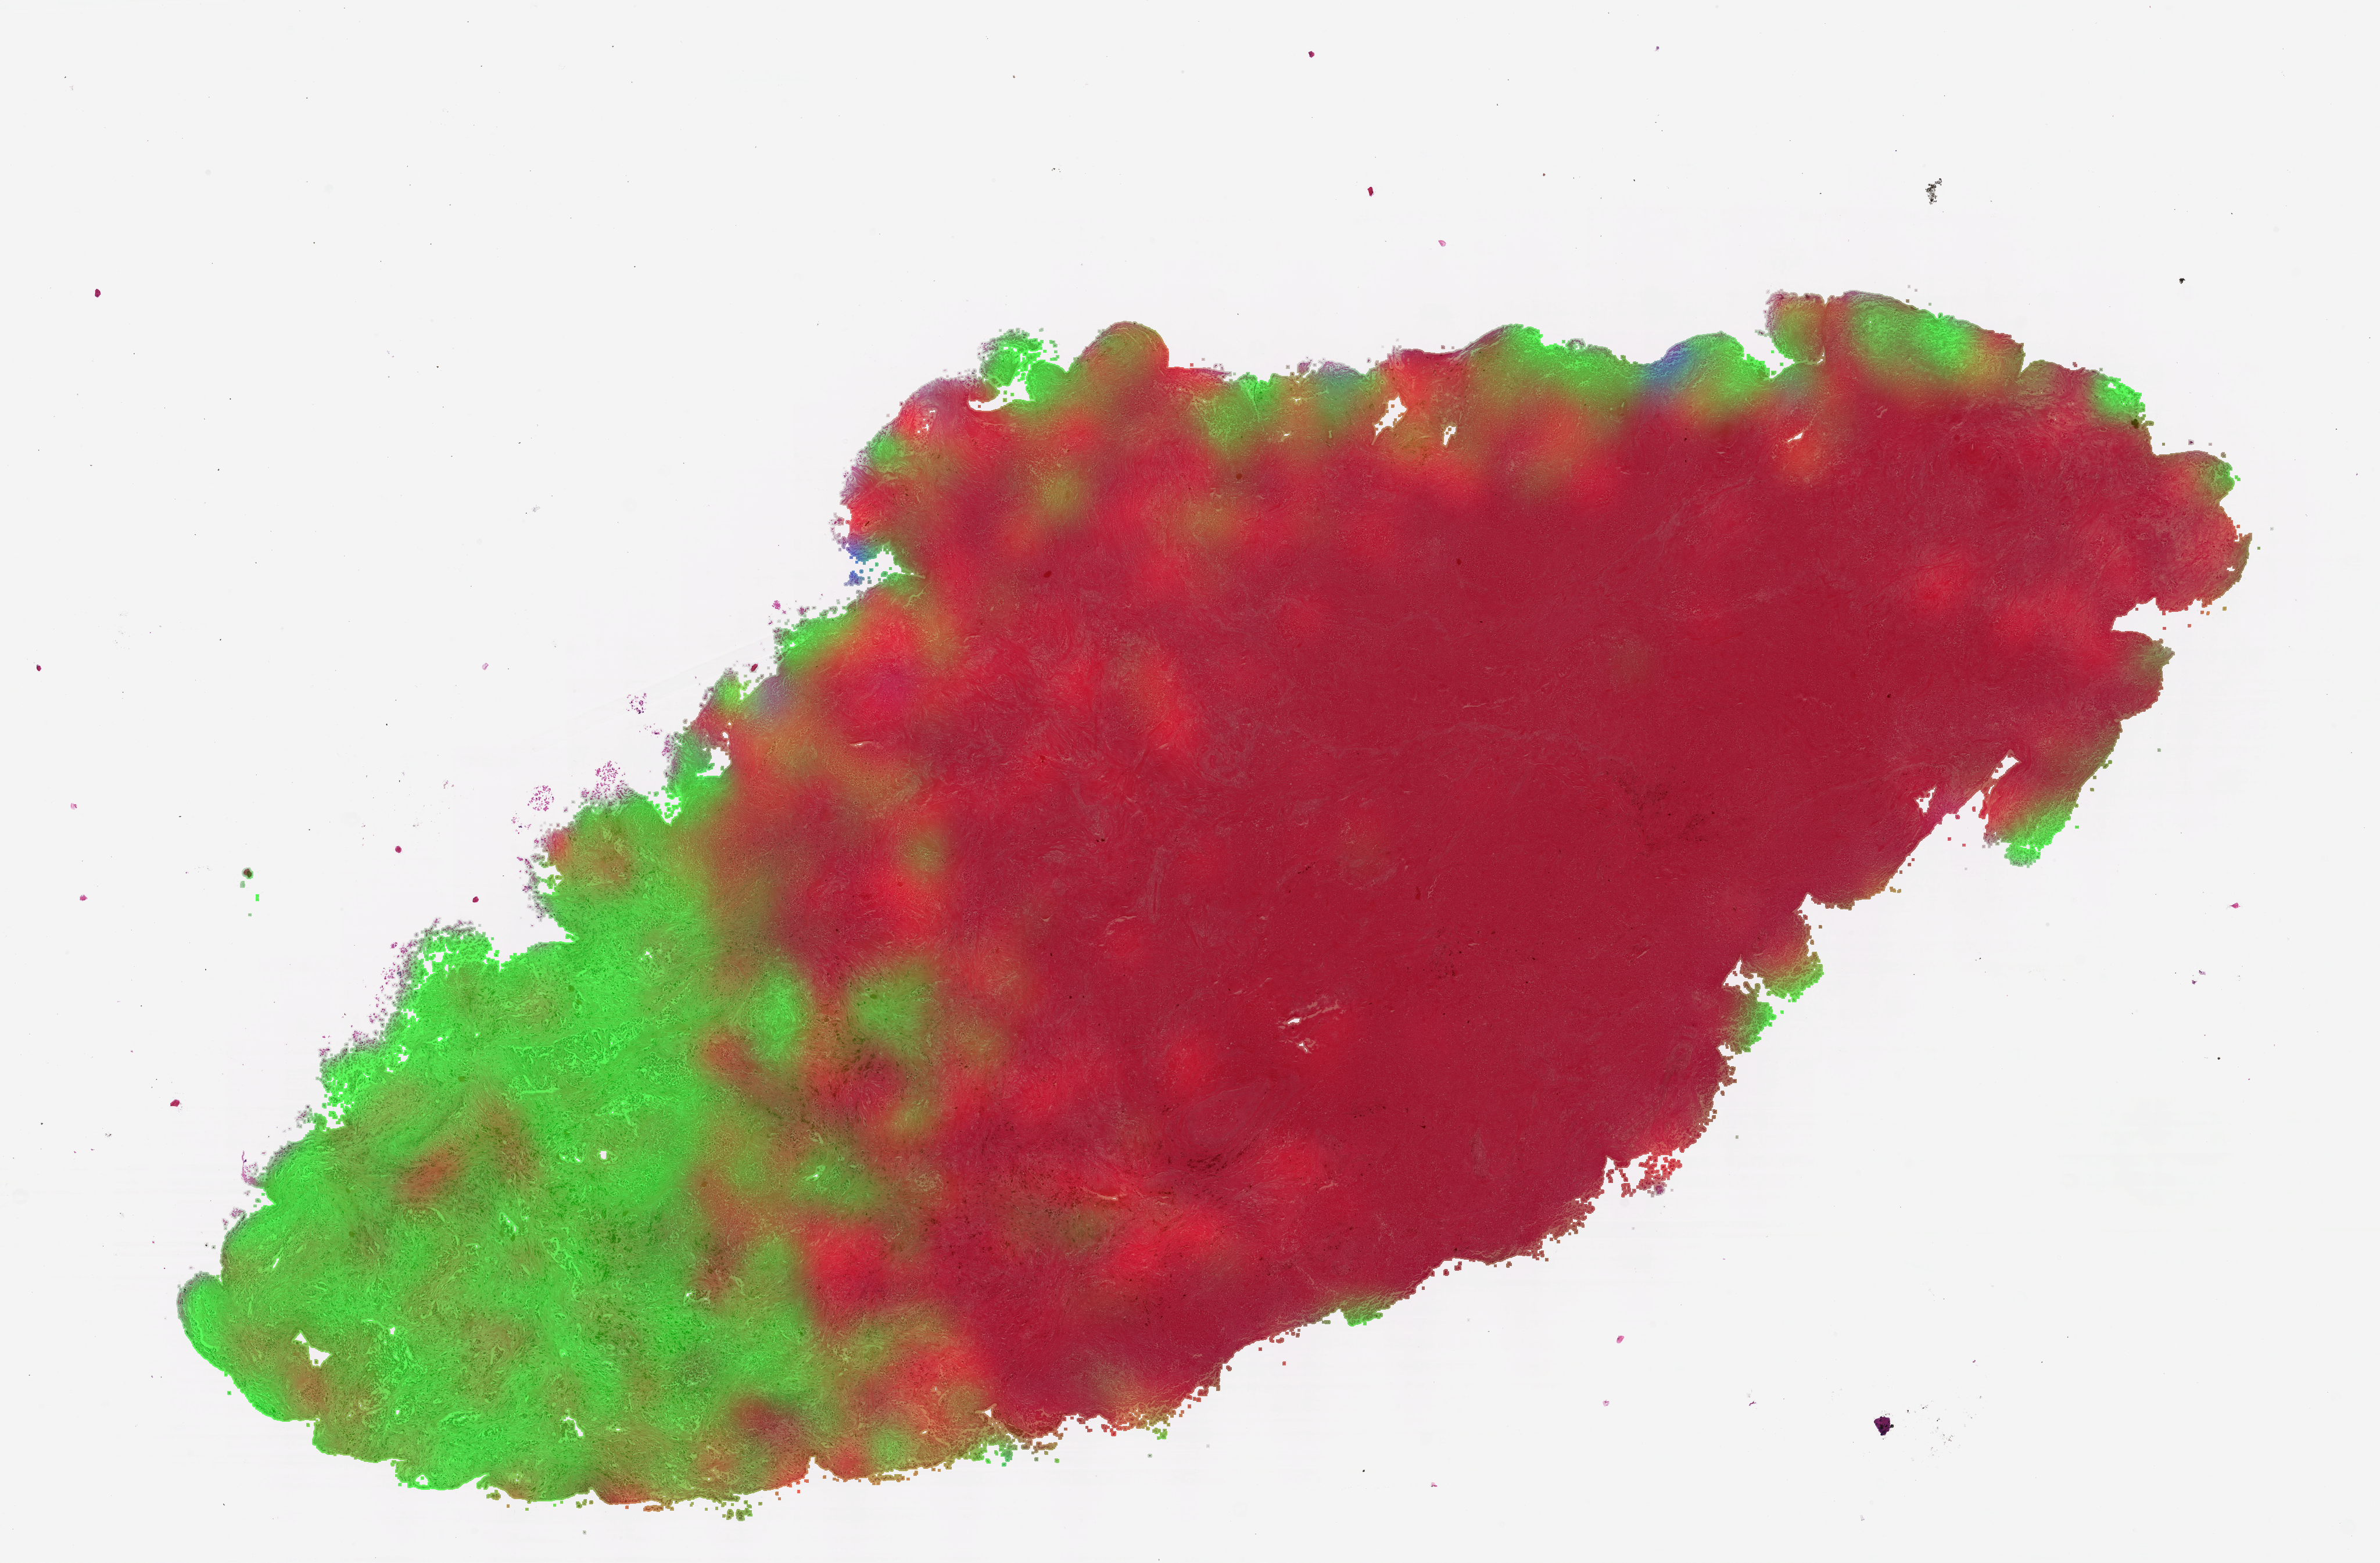
\includegraphics[width=\textwidth]{chapters/figures/lchai_v2_KEAP1_TCGA-49-AAR9_pattern_overlay.png}
\end{minipage}\hfill
\begin{minipage}[t]{0.48\textwidth}
\centering
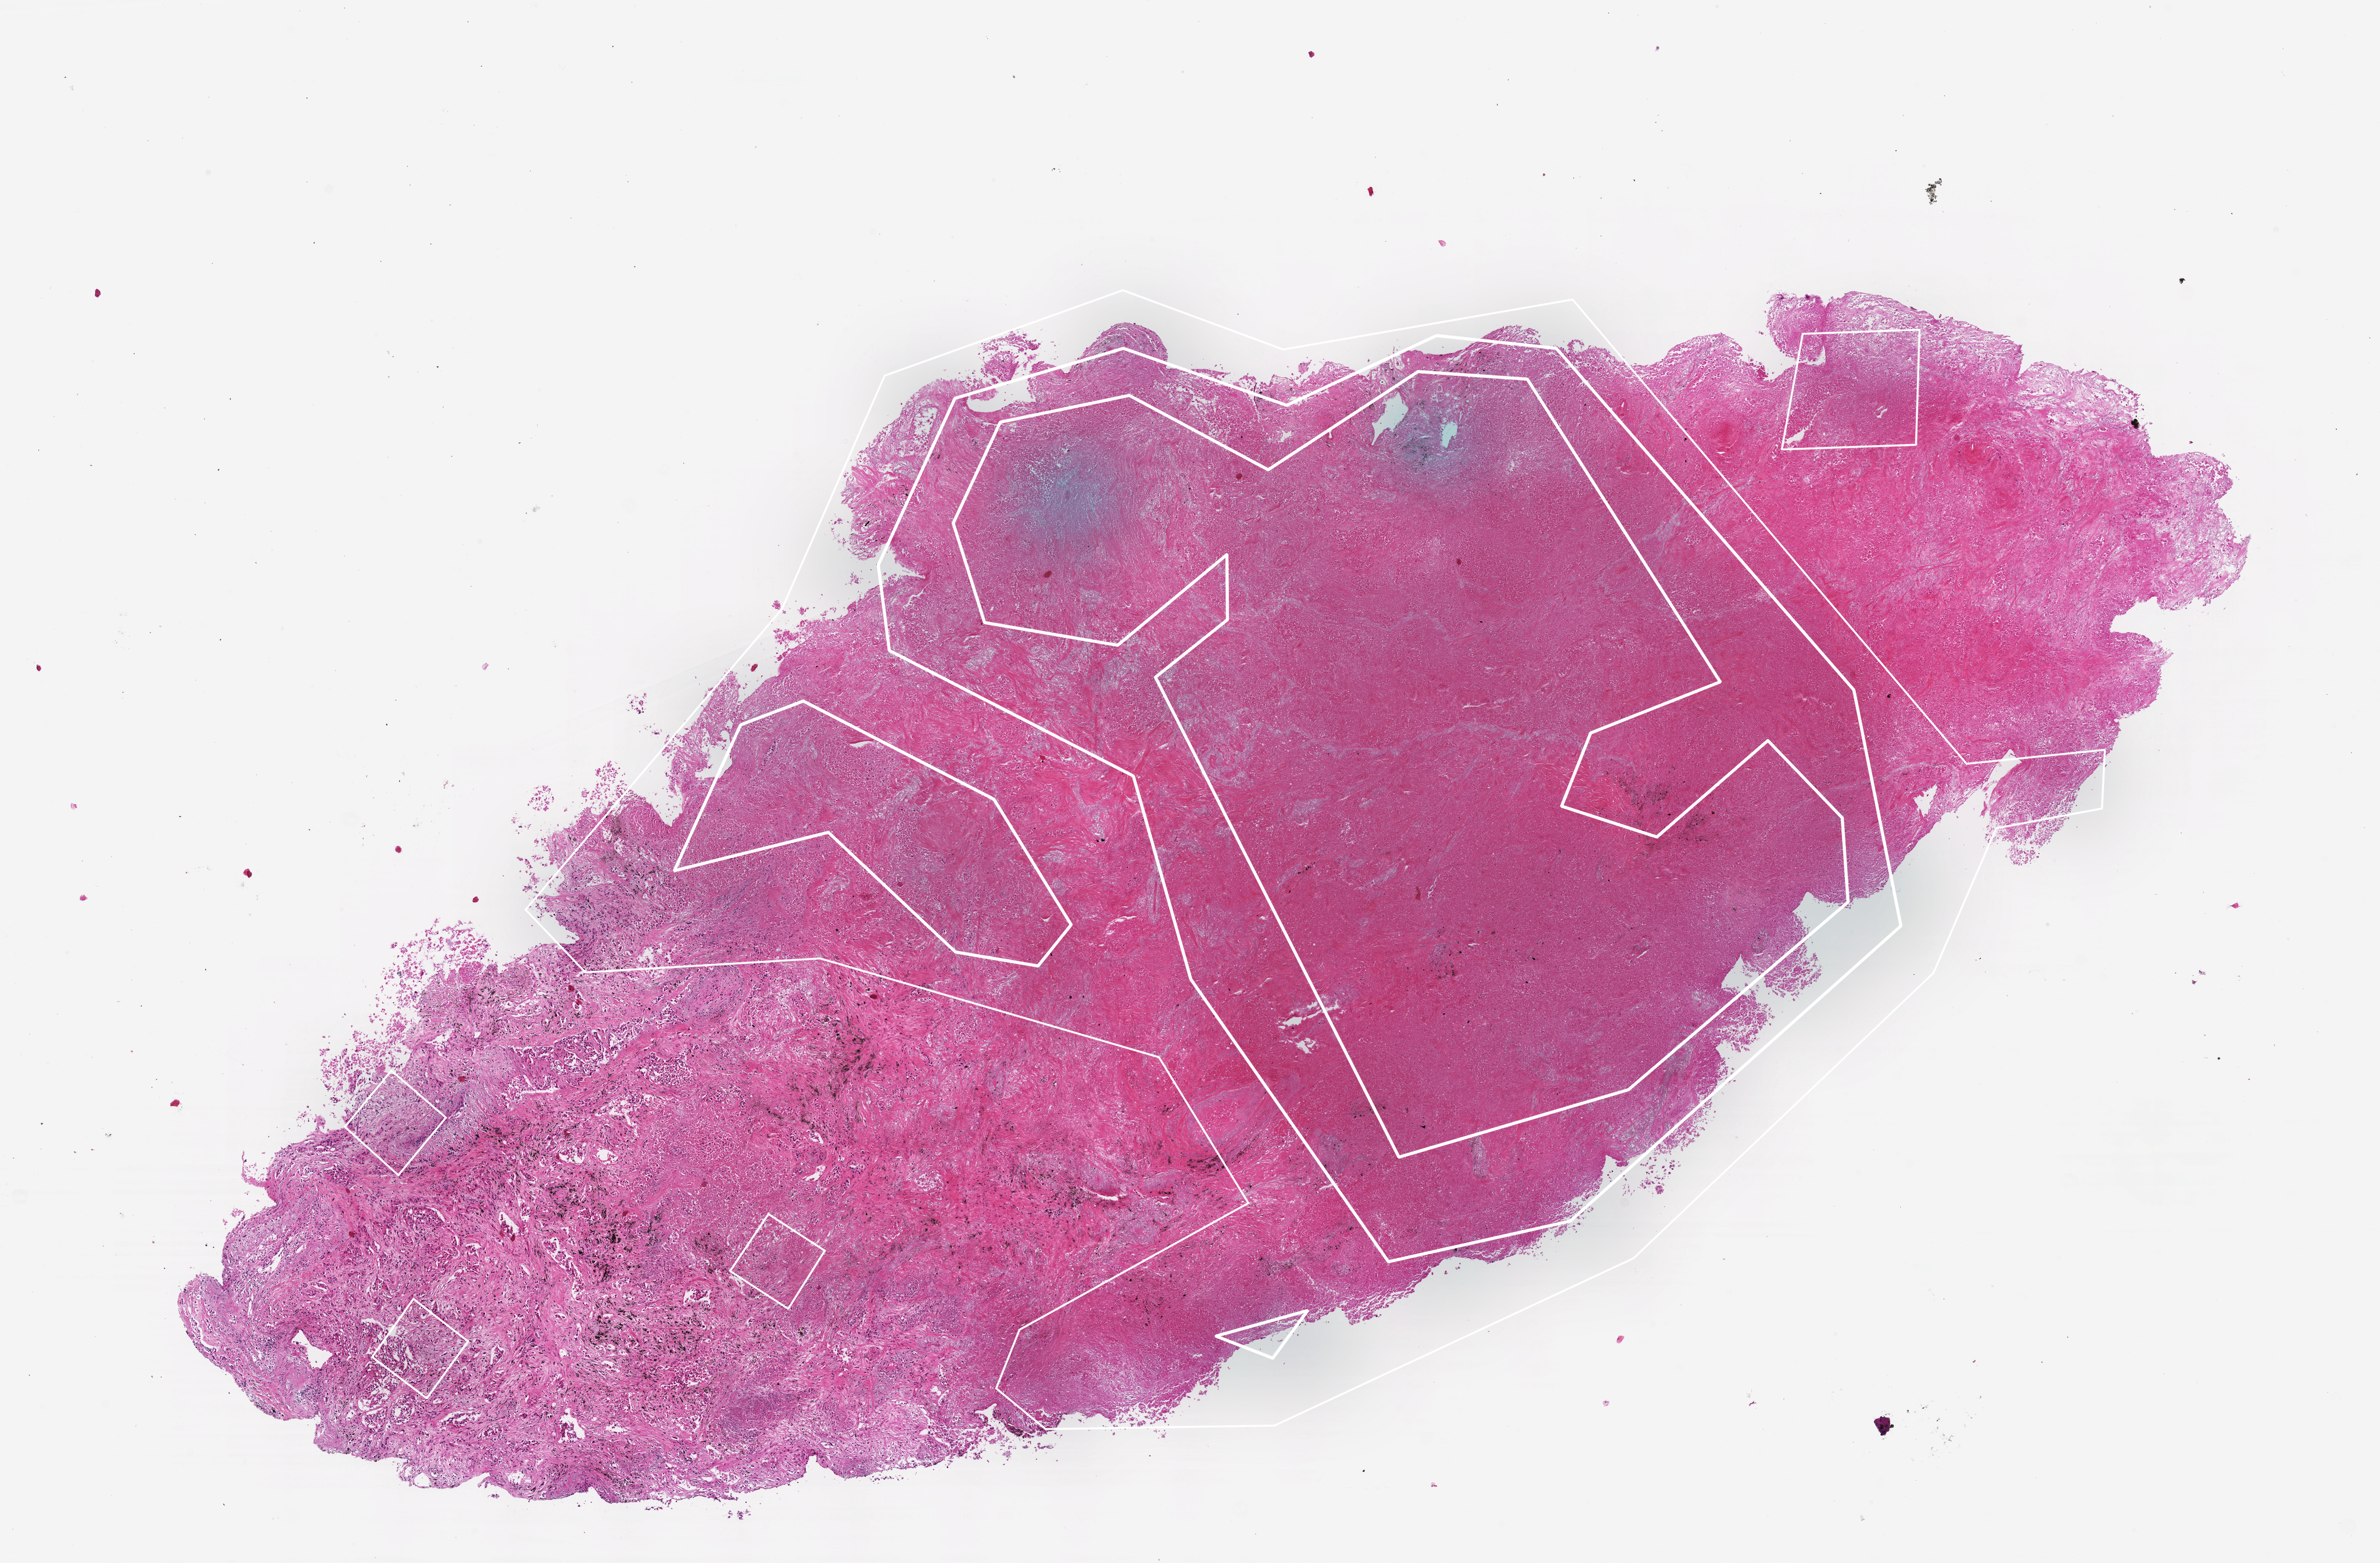
\includegraphics[width=\textwidth]{chapters/figures/lchai_v2_KEAP1_TCGA-49-AAR9_attention_map.png}
\end{minipage}\\[6pt]
\begin{minipage}[t]{0.48\textwidth}
\centering
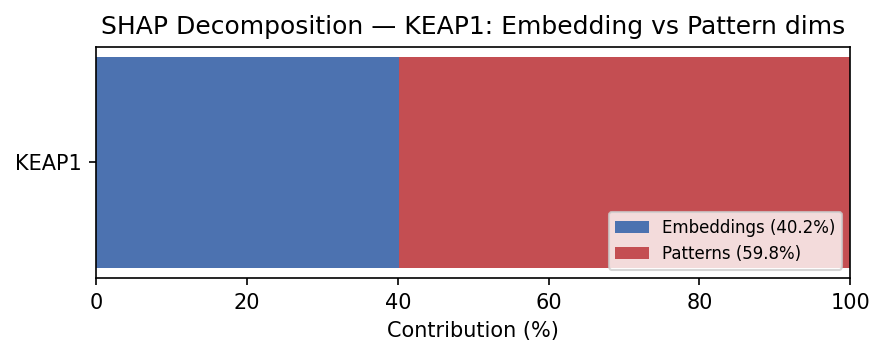
\includegraphics[width=\textwidth]{chapters/figures/shap_decomp_KEAP1_49_AAR9_bar.png}
\end{minipage}\hfill
\begin{minipage}[t]{0.48\textwidth}
\centering
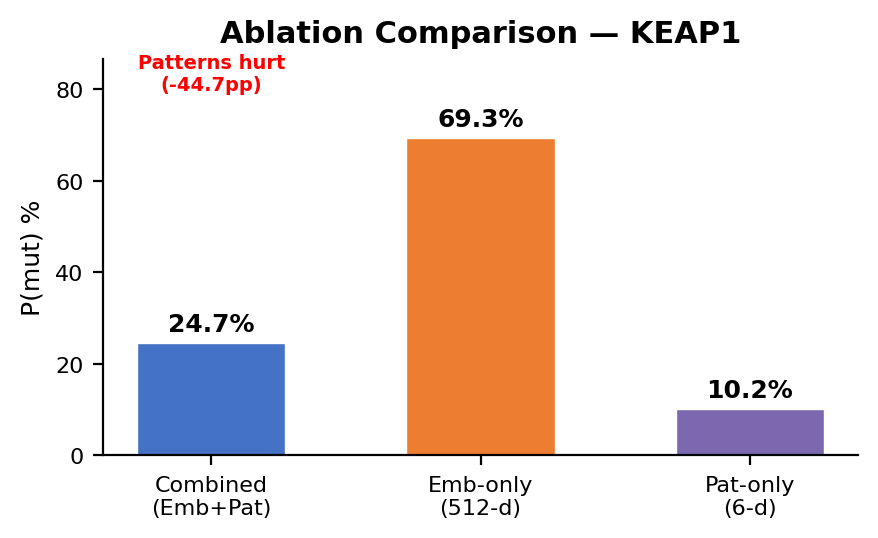
\includegraphics[width=\textwidth]{chapters/figures/ablation_KEAP1_49_AAR9.png}
\end{minipage}
\caption[LCHAI~v2.0 interpretability: KEAP1 (TCGA-49-AAR9)]{%
    LCHAI~v2.0 interpretability for KEAP1-mutant slide TCGA-49-AAR9
    (P(mut)~$= 0.247$, PI-ABMIL; population-level: Inconclusive).
    \textbf{Top left}: Pattern overlay---solid-dominant (64.14\%, dark red)
    with micropapillary (20.68\%, green) and acinar (14.18\%, red).
    \textbf{Top right}: ABMIL attention map---broad and diffuse.
    \textbf{Bottom left}: SHAP decomposition---40\% embedding / 60\% pattern.
    \textbf{Bottom right}: Ablation---Combined (24.7\%) drops sharply from
    Emb-only (69.4\%): the heterogeneous pattern composition introduces
    strong interference ($-44.7$\,pp).}
\label{fig:attn_keap1_tp}
\end{figure}

\textbf{Interpretation.}
KEAP1 mutations perturb an internal biochemical control loop---%
the KEAP1--NRF2 oxidative-stress response, which functions as a
negative-feedback controller the cell uses to defend itself
against toxic metabolites~\cite{tcga2014luad}.
By the analogy of the previous case studies, this is a
runtime-internal regulator: it modulates how the cell handles
stress, not how the tumour organises itself in space.
The disruption is therefore biochemical, not morphological, so---%
unlike TP53 or KRAS---there is no consistent visual fingerprint
at the slide level for a vision model to condition on:
the conditional input distribution
$p(\text{slide}\,|\,\text{KEAP1 mutant})$ has no robust support
in any single growth pattern.
DNA sequencing confirms the KEAP1 mutation on this slide, yet
the model returns only $P(\text{mut}) = 0.247$---a
\textbf{false negative}.
Three factors explain why:

\begin{enumerate}
    \item \textbf{No robust tissue pattern correlate exists in
    the literature.}
    Unlike EGFR (Section~\ref{sec:eval:interp:attention}, where
    lepidic and papillary patterns are \emph{known to associate}
    with the mutation and are simply absent on the
    EGFR false-negative slide), KEAP1 lacks a discriminative
    histological signature: although Li
    et~al.~\cite{li2011keap1papillary} reported a weak
    association with papillary adenocarcinoma (a finger-shaped
    growth pattern) in a small cohort, comprehensive reviews of
    the correspondence between DNA-level mutations and tissue
    growth patterns in LUAD~\cite{hung2020molecular} do not
    include KEAP1 among genes with a recognised pattern
    signature, in contrast to genes such as EGFR (acinar /
    papillary patterns), ALK (solid / cribriform---sieve-like
    patterns), or NRG1 (the invasive mucinous subtype).
    There is therefore no specific visual cue the pattern channel
    could attach to on this---or any other---KEAP1 slide; this
    case is the slide-level signature of the population-level
    \emph{spread} sub-case of regime~B
    (engaged-but-unproductive) of Finding~6
    (Section~\ref{sec:eval:mutation:finding6}), which provides
    \emph{model-internal} evidence consistent with the absence of
    a robust morphological correlate in the external literature.

    \item \textbf{The pattern channel is actively destructive on
    this slide ($-44.7$\,pp), flipping the decision.}
    The slide is morphologically heterogeneous (solid 64.14\%,
    micropapillary 20.68\%, acinar 14.18\%) with no dominant
    pattern, and the ablation panel of
    Figure~\ref{fig:attn_keap1_tp} shows the consequence: the
    Embeddings-only model reaches $69.4\%$---\emph{above} the
    $0.5$ decision threshold, which alone would have made this
    slide a true positive---while the Combined model drops to
    $24.7\%$, a $-44.7$\,pp penalty that crosses the threshold
    and produces the false negative.
    The mechanism is precisely the regime~B \emph{spread}
    sub-case's pair-bias mismatch: with a heterogeneous tile mix
    and no documented KEAP1 pattern indicator, the Choquet
    branch finds no superadditive pair to lock onto and
    contributes noise that drowns the embedding pathway's signal.
    PI-ABMIL, whose graded pattern memberships do not assume any
    pair structure, beats both B2 and FC-MIL on KEAP1 at the
    population level (Table~\ref{tab:p_vs_b2}) and is the
    selected method on this slide; on this particular case, even
    PI-ABMIL cannot fully overcome the absence of a learnable
    pattern correlate, leaving $P = 0.247 < 0.5$.

    \item \textbf{KEAP1 is population-level Inconclusive, with
    heavily overlapping score distributions.}
    KEAP1 has a prevalence of only $14.3\%$ in the cohort
    (Figure~\ref{fig:auroc_by_gene}, caption) and a mean 5-fold
    AUROC of $0.610$, which is \emph{below} the
    Hosmer--Lemeshow $0.70$ threshold for acceptable
    discrimination~\cite{hosmer2000applied}---hence the
    Inconclusive label of Table~\ref{tab:viz_folds}.
    Mechanically, AUROC $= 0.610$ means that around $39\%$ of
    (positive, negative) slide pairs are mis-ranked, a
    substantially heavier overlap of mutant and wild-type score
    distributions than for EGFR (AUROC $= 0.701$, around $30\%$
    misranking; the same overlap argument visualised in
    Figure~\ref{fig:egfr_score_overlap} applies here \emph{a
    fortiori}).
    A KEAP1-mutant slide carrying no specific visual anchor is
    therefore \emph{statistically expected} to fall into the
    false-negative tail of the mutant score distribution---which
    is exactly what happens at $P = 0.247$.
\end{enumerate}

This case is also the most extreme demonstration in the cohort
of a recurring lesson of the interpretability framework:
\textbf{a model can pay strong attribution to an input channel
and still be hurt by it}.
SHAP measures \emph{sensitivity}---how much the prediction
moves when the channel's value changes---while channel ablation
measures \emph{causal contribution}: whether the channel's
presence improves the prediction at all.
The two need not agree, and KEAP1 is the cohort case where they
disagree most.
Figure~\ref{fig:keap1_attention_vs_utility} makes the divergence
visible across the six representative slides: KEAP1 sits alone
in the lower-right quadrant, combining the highest pattern
attribution ($60\%$) with the largest negative ablation delta
($-44.7$\,pp), well below every other gene and far from the
diagonal that would be expected if SHAP attribution tracked
actual usefulness.

\begin{figure}[!htbp]
    \centering
    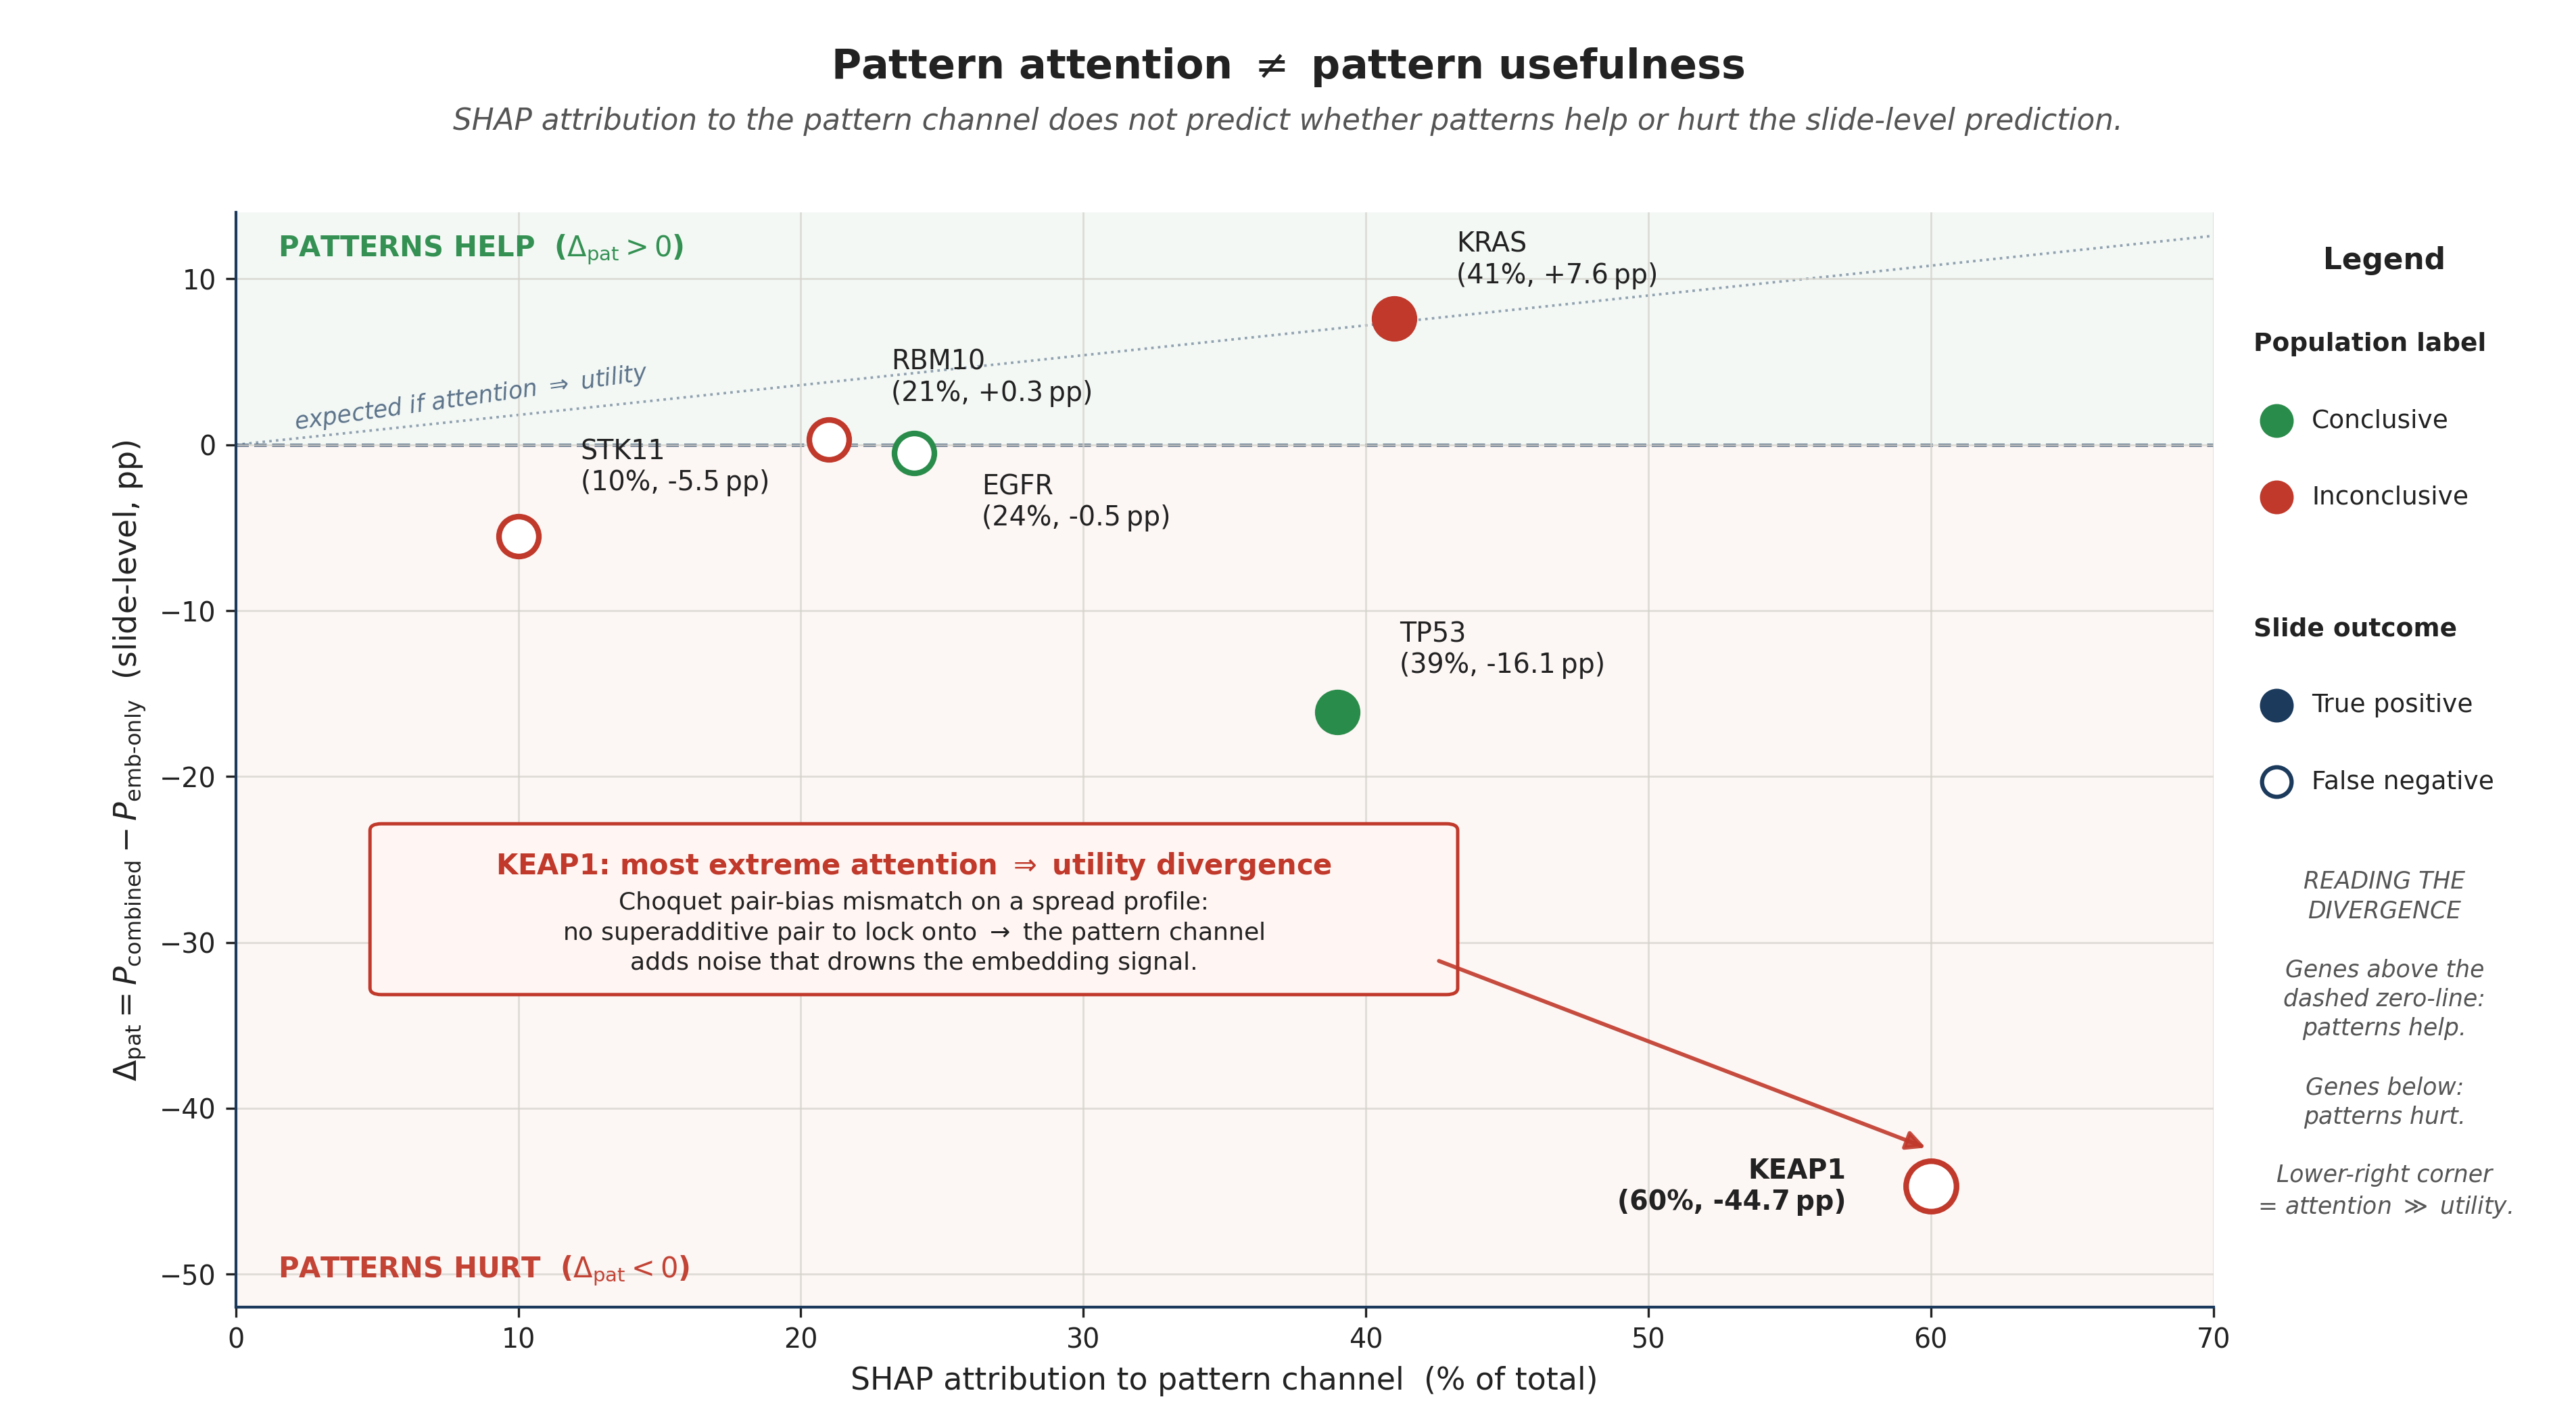
\includegraphics[width=\textwidth]{chapters/figures/keap1_attention_vs_utility.png}
    \caption[KEAP1: pattern attention vs.\ pattern usefulness across
    the six representative slides]{%
    \textbf{Pattern attention is not the same as pattern
    usefulness.}
    For each of the six representative slides
    (Table~\ref{tab:enrichment_summary}), the horizontal axis shows
    the SHAP attribution of the prediction to the pattern channel
    and the vertical axis shows the slide-level pattern ablation
    delta $\Delta_{\mathrm{pat}} = P_{\mathrm{combined}} -
    P_{\mathrm{emb\text{-}only}}$ (in pp; bottom-right panels of
    Figures~\ref{fig:attn_tp53_tp}--\ref{fig:attn_rbm10_tp}).
    Marker colour encodes the population-level Conclusive/%
    Inconclusive label (cohort mean 5-fold AUROC, Hosmer--Lemeshow
    threshold $\geq 0.70$); filled markers are slide-level true
    positives, hollow markers are false negatives.
    The dotted diagonal sketches the (counterfactual) trend in
    which attention to patterns would translate proportionally
    into improved prediction.
    KEAP1 is the extreme outlier: the highest pattern attention
    in the cohort coincides with the largest negative
    $\Delta_{\mathrm{pat}}$, the slide-level signature of the
    regime~B \emph{spread} sub-case's pair-bias mismatch
    (Finding~6, Section~\ref{sec:eval:mutation:finding6}).
    KRAS is the only point in the upper half: a moderate-attention
    case where patterns measurably help.}
    \label{fig:keap1_attention_vs_utility}
\end{figure}

\paragraph{Why LCHAI~v2.0 does not switch to the Emb-only model
for this slide.}
The ablation panel of Figure~\ref{fig:attn_keap1_tp} (bottom
right) shows that the Embeddings-only counterfactual model
$f_{\text{B2}}$ would have produced $P_{\text{emb}} = 69.4\%$
on TCGA-49-AAR9---above the $0.5$ decision threshold, a
\emph{true positive}---whereas the deployed PI-ABMIL model
returns $P_{\text{comb}} = 24.7\%$, a false negative.
This is the canonical case for which the arbitration argument
of Section~\ref{sec:meth:interp:gene_vs_slide_selection}
(Figure~\ref{fig:per_slide_arbitration_fails}) was formulated:
a per-slide override to $f_{\text{B2}}$ would convert the false
negative into a true positive on this slide, yet LCHAI~v2.0
does not perform that override because the gene-level rule is
fixed before any test slide is examined and the four arguments
against per-slide arbitration apply with particular force at
KEAP1's $14.3\%$ prevalence
(Table~\ref{tab:mutation_prevalence}), where the false-positive
penalty of a $\max$-of-experts rule typically cancels the
recovered false negatives.
On KEAP1, PI-ABMIL is the per-gene best-in-expectation model
($+0.013$ AUROC over B2; Table~\ref{tab:p_vs_b2}), so its
deployment minimises expected misranking risk across the cohort
even when it produces this individual false negative.

This trade-off---accepting individual slide-level false
negatives to preserve cohort-level calibration---is discussed
as a methodological limitation in
Section~\ref{sec:disc:lim:method}, and a label-free
mixture-of-experts gate as a future-work extension in
Section~\ref{sec:disc:future:moe_gate}.
The Level~5 ablation panel of LCHAI~v2.0 thus surfaces the
counterfactual $P_{\text{emb}} = 69.4\%$ as an
\emph{interpretability} signal---a transparency cue for the
clinician that pattern-channel interference is the proximal
cause of this false negative---rather than as a runtime override.


\subsubsection{RBM10: RNA Splicing Factor with Minimal Morphological
Footprint}
\label{sec:eval:tcga:rbm10}

Figure~\ref{fig:attn_rbm10_tp} presents the RBM10 analysis for slide
TCGA-78-7148, an RBM10-mutant case predicted with very low mutation
probability (P(mut)~$= 0.017$, method: FC-MIL;
population-level: \textbf{Inconclusive}, cohort mean 5-fold
AUROC~$= 0.661 < 0.70$; Table~\ref{tab:viz_folds}).
As established in the case-study preamble
(Section~\ref{sec:eval:interp:attention}), the slide-level
evidence below does \emph{not} re-label this slide; it explains
\emph{why} the cohort AUROC sits where it does.
The slide is $88.69\%$ micropapillary-classified with minor acinar
($8.15\%$) and solid ($2.57\%$) content.
The SHAP decomposition shows $79\%$ embedding / $21\%$ pattern
(fuzzy classification: \emph{Embedding-Led}), and the Choquet
Shapley values are nearly uniform across all six patterns (range
$0.1664$--$0.1671 \approx 1/6$; fuzzy profile: \emph{Uniform}):
no single pattern carries discriminative signal for RBM10 on this
slide.

At the population level RBM10 sits in regime~B
(\emph{engaged-but-unproductive}) of Finding~6
(Section~\ref{sec:eval:mutation:finding6}), specifically as the
\emph{collapse-to-prior} sub-mechanism of the ontology-coverage
taxonomy (RQ2(ii); Figure~\ref{fig:signal_tree}).
FC-MIL does beat B2 by $+0.019$ AUROC
($0.661$ vs $0.642$; Tables~\ref{tab:mutation_luad}
and~\ref{tab:p_vs_b2})---the largest FC-MIL gain in the cohort---%
but the Choquet branch is itself empty: on the seed-42 trained
model the singleton spread is $0.0007$ with all $|I_{kl}| < 0.01$
(Section~\ref{sec:eval:interp:choquet}).
The lift therefore originates in the shared embedding pathway,
not in any pattern interaction; equivalently, FC-MIL on RBM10
behaves like an ensemble whose second branch is silent, and the
ensemble's slight lift is the noise-reduction of the active
branch rather than the silent one finding new signal.
The engagement map of Figure~\ref{fig:choquet_variance_map}
records the unstable exploration of the empty branch
($\Delta\mathrm{AUROC} = +0.019$, $\Delta\sigma = +0.009$): the
optimiser latches onto a different pair each fold without ever
locking onto a stable visual indicator, consistent with a
feature space that carries no discriminative signal.
RBM10 is therefore an \emph{architectural negative control}---%
the cleanest-null profile in the cohort
(per-slide $\Delta_{\mathrm{pat}} = +0.3$\,pp with all three
ablation variants collapsing near the prior;
Figure~\ref{fig:rbm10_cleanest_null})---against which KRAS's
IMA-proxy reading (Finding~4,
Figure~\ref{fig:kras_two_routes}) can be read as the only
genuine cross-term signal in the cohort.

\begin{figure}[ht!]
\centering
\begin{minipage}[t]{0.48\textwidth}
\centering
\includegraphics[width=\textwidth]{chapters/figures/lchai_v2_RBM10_TCGA-78-7148_pattern_overlay.png}
\end{minipage}\hfill
\begin{minipage}[t]{0.48\textwidth}
\centering
\includegraphics[width=\textwidth]{chapters/figures/lchai_v2_RBM10_TCGA-78-7148_attention_map.png}
\end{minipage}\\[6pt]
\begin{minipage}[t]{0.48\textwidth}
\centering
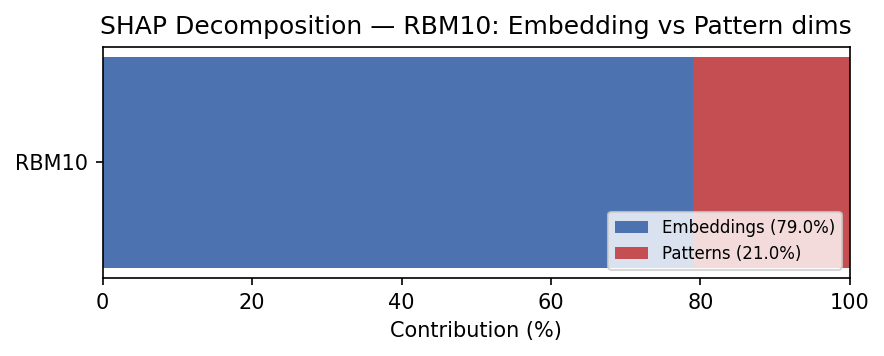
\includegraphics[width=\textwidth]{chapters/figures/shap_decomp_RBM10_78_7148_bar.png}
\end{minipage}\hfill
\begin{minipage}[t]{0.48\textwidth}
\centering
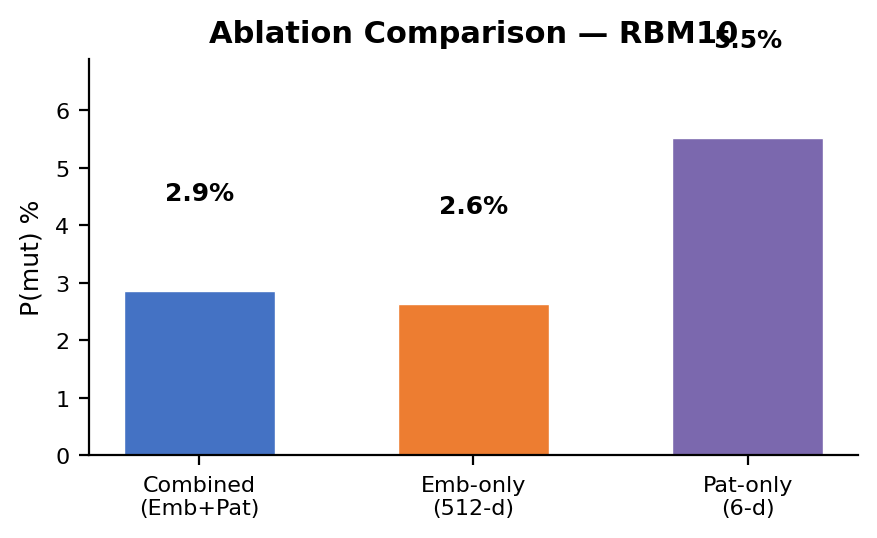
\includegraphics[width=\textwidth]{chapters/figures/ablation_RBM10_78_7148.png}
\end{minipage}
\caption[LCHAI~v2.0 interpretability: RBM10 (TCGA-78-7148)]{%
    LCHAI~v2.0 interpretability for RBM10-mutant slide TCGA-78-7148
    (P(mut)~$= 0.017$, FC-MIL; population-level: Inconclusive).
    \textbf{Top left}: Pattern overlay---micropapillary-dominant (88.69\%, green)
    with acinar foci (8.15\%, red).
    \textbf{Top right}: ABMIL attention map---scattered, no clear focus.
    \textbf{Bottom left}: SHAP decomposition---79\% embedding / 21\% pattern.
    \textbf{Bottom right}: Ablation---all three models produce near-zero
    probabilities (2.9\%, 2.6\%, 5.5\%), consistent with the
    absence of a robust standalone morphological correlate for
    RBM10 (see Factor~1 below).}
\label{fig:attn_rbm10_tp}
\end{figure}

\textbf{Interpretation.}
From a vision model's vantage point, RBM10 is a worst-case
label: the gene encodes a protein that regulates \emph{RNA
splicing}, the step at which a cell edits its genetic
instructions before they are translated into
proteins~\cite{bechara2013rbm10}.
This is a sub-cellular regulatory step that rearranges
intermediate transcripts but does not, on its own, reorganise the
externally observable morphology the slide records.
Concretely, the only signal a histopathology model ever sees is
the H\&E-stained slide, i.e.\ the morphology that the cell
\emph{produces}; an upstream splicing-level edit that does not
visibly reorganise that morphology leaves no trace in the model's
input distribution---the population-level expression of the
\emph{collapse-to-prior} regime that classifies RBM10 within the
ontology-coverage taxonomy of
RQ2(ii)~(Figure~\ref{fig:signal_tree}).
Unlike TP53 or KRAS, then, no robust standalone tissue pattern
flags ``this tumour has an RBM10 mutation'' (the literature
evidence is reviewed in Factor~1 below): the conditional
distribution $p(\text{slide}\,|\,\text{RBM10 mutant})$ is
empirically indistinguishable from $p(\text{slide}\,|\,\text{wild-type})$
once stage and co-mutation context are stripped away.
DNA sequencing nonetheless confirms the RBM10 mutation on this
slide, and the model returns $P(\text{mut}) = 0.017$---a
\textbf{false negative}.
This is a genuine missing-signal case rather than a model defect,
and the three factors below decompose why.

\begin{enumerate}
    \item \textbf{No robust standalone histological correlate.}
    Like KEAP1 (the previous case study), RBM10 lacks a
    discriminative pattern signature in lung adenocarcinoma
    (LUAD).
    Cao et~al.~\cite{cao2024rbm10egfr} did report that RBM10
    mutations co-occur with EGFR mutations in
    \emph{lepidic-pattern ground-glass nodules}---small,
    early-stage tumours that grow along the alveolar walls
    and appear as hazy, semi-transparent regions on CT
    imaging---but that association is conditional on two
    auxiliary variables (early stage \emph{and} an EGFR
    co-mutation), so it behaves as a context-dependent
    feature interaction, not as a standalone correlate of
    RBM10 status.
    Hung's review of the correspondence between DNA-level
    mutations and LUAD growth patterns~\cite{hung2020molecular}
    likewise does not list RBM10 among genes with a recognised
    pattern signature.
    The biological mechanism differs from KEAP1's---RBM10
    perturbs how genetic instructions are parsed and edited,
    whereas KEAP1 perturbs an internal feedback-control
    loop---but, from the model's perspective, the consequence
    is identical: no class-conditional shift in slide
    morphology.
    The Choquet branch reflects this directly.
    Its per-pattern Shapley values on this slide are uniform
    ($\phi_k \approx 1/6$, i.e.\ the maximum-entropy point of
    the six-pattern simplex)---the signature of a label on
    which the Choquet aggregator has nothing to anchor on
    (Figure~\ref{fig:rbm10_cleanest_null}, panel a).

    \item \textbf{All three ablation pathways collapse to
    near-zero on this slide.}
    The bottom-right panel of
    Figure~\ref{fig:attn_rbm10_tp} reports the predicted
    mutation probability under each information channel
    individually:
    Combined~$= 2.9\%$, Emb-only~$= 2.6\%$,
    Pat-only~$= 5.5\%$.
    Unlike KEAP1, where the embedding-only ablation reached
    $69.4\%$ and the pattern channel \emph{flipped} the
    decision by $-44.7$\,pp---a clear case in which each
    channel carried a signal that the other suppressed---here
    \emph{neither} channel recovers RBM10: the CTransPath
    foundation-model embedding finds no fine-grained texture
    signature, and the WHO-pattern channel finds no
    discriminative composition
    (Figure~\ref{fig:rbm10_cleanest_null}, panel b, contrasts
    this collapse with the productive KEAP1 case).
    This is the slide-level realisation of regime~B's
    \emph{engaged-but-unproductive} reading of RBM10
    (Finding~6, Section~\ref{sec:eval:mutation:finding6}):
    the Choquet branch trains over a feature space that carries
    no RBM10-discriminative signal, latches onto a different
    pair of patterns at each cross-validation fold without
    ever locking onto a stable visual indicator, and on this
    test slide degenerates to a near-uniform aggregation that
    collapses with the rest of the prediction towards the prior.

    \item \textbf{RBM10 is population-level Inconclusive
    with the most extreme AUROC--AUPRC gap of the cohort.}
    RBM10 has a cohort prevalence of only $5.4\%$ ($37$
    mutated slides, the lowest of the six target genes) and a
    mean 5-fold AUROC of $0.661$, below the
    Hosmer--Lemeshow Conclusive threshold of $0.70$ used in
    this thesis to gate slide-level interpretability claims.
    Read operationally, AUROC $= 0.661$ means that for
    roughly $34\%$ of (mutant, wild-type) slide pairs the
    wild-type slide receives the higher mutant score---i.e.\
    the model \emph{ranks} the pair the wrong way around---and
    the low prevalence pushes precision down even further:
    AUPRC drops to approximately $0.17$
    (Figure~\ref{fig:auprc_by_gene};
    Section~\ref{sec:disc:lim:method},
    Chapter~\ref{ch:discussion}).
    Combined, these two facts mean that an RBM10-mutant slide
    with no specific visual anchor is statistically expected
    to fall deep into the false-negative tail of the mutant
    score distribution---which is exactly what happens at
    $P = 0.017$
    (Figure~\ref{fig:rbm10_cleanest_null}, panel d,
    summarises the cohort statistics that drive this
    expectation).
\end{enumerate}

\begin{figure}[ht!]
\centering
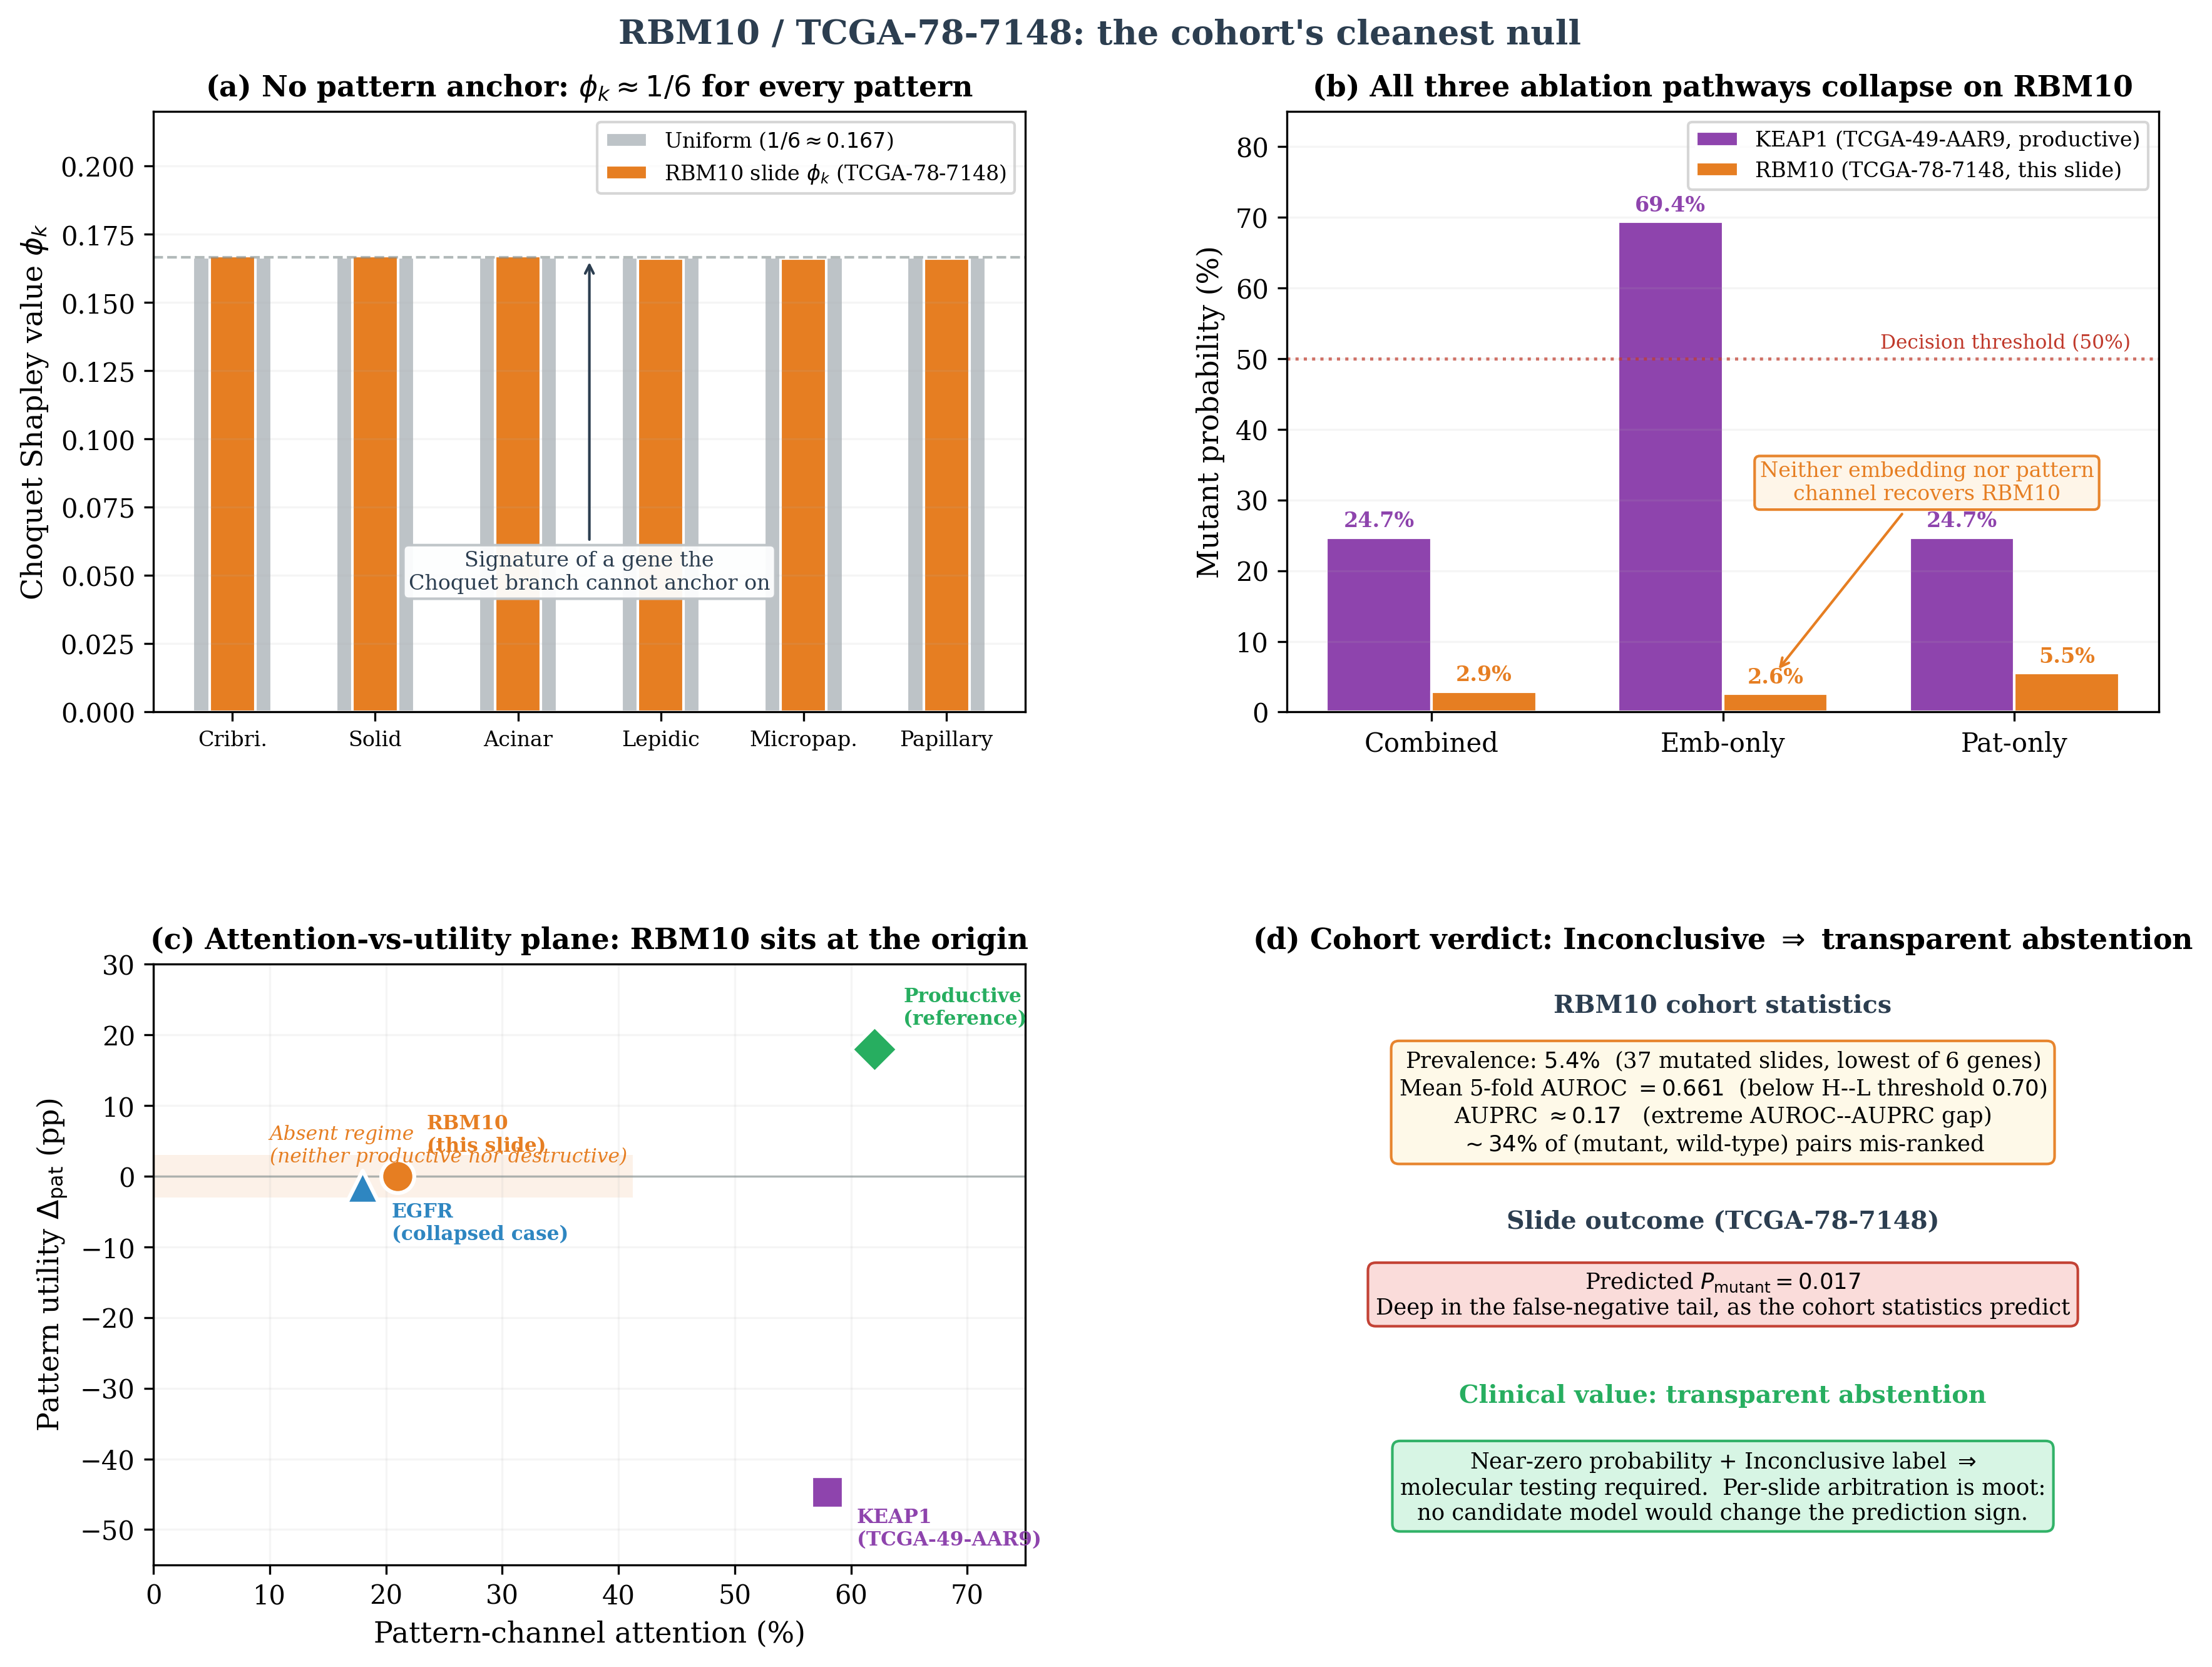
\includegraphics[width=\textwidth]{chapters/figures/rbm10_cleanest_null.png}
\caption[RBM10/TCGA-78-7148: the cohort's cleanest null]{%
    Synthesis of the three factors discussed above for
    RBM10-mutant slide TCGA-78-7148.
    \textbf{(a)} Choquet Shapley singletons are uniform at
    $\phi_k \approx 1/6$ across all six WHO patterns---no
    pattern anchor (Factor~1).
    \textbf{(b)} All three ablation pathways (Combined~$2.9\%$,
    Emb-only~$2.6\%$, Pat-only~$5.5\%$) collapse far below the
    decision threshold, in contrast with the productive KEAP1
    case (TCGA-49-AAR9), where the embedding pathway alone
    reaches $69.4\%$ (Factor~2).
    \textbf{(c)} Attention-vs-utility plane: RBM10 sits at the
    origin ($\sim 21\%$ pattern attention,
    $\Delta_{\text{pat}} \approx 0$)---the slide-level
    signature of an absent pattern channel, distinct from the
    productive--destructive KEAP1 regime in the lower-right
    (cf.\ Figure~\ref{fig:keap1_attention_vs_utility}).
    \textbf{(d)} Cohort verdict: $5.4\%$ prevalence, mean
    5-fold AUROC~$= 0.661 < 0.70$, AUPRC~$\approx 0.17$;
    $P_{\text{mutant}} = 0.017$ falls deep in the
    false-negative tail (Factor~3), which the
    population-level Inconclusive label translates into
    transparent abstention---molecular testing is required.}
\label{fig:rbm10_cleanest_null}
\end{figure}

This case is the cohort's \emph{cleanest null}: on a slide where
neither the pattern channel nor the embedding channel recovers any
RBM10 signal, the framework's clinical---and engineering---value
lies in \emph{transparent abstention}.
Concretely, the model returns a near-zero probability, the
population-level Inconclusive label warns the user that molecular
testing is required, and the slide-level evidence makes the
cohort failure mode concrete: no morphological correlate, no
fold-stable pair, no embedding anchor
(Figure~\ref{fig:rbm10_cleanest_null} synthesises the three
factors and the resulting abstention verdict in a single view).
The same conclusion is reached from a different angle by the
attention-vs-utility plane:
Figure~\ref{fig:keap1_attention_vs_utility}---and panel~(c) of
Figure~\ref{fig:rbm10_cleanest_null}---place RBM10 near the
origin ($21\%$ pattern attention,
$\Delta_{\text{pat}} \approx 0$), meaning the pattern channel
is neither productive nor destructive on this case but simply
absent: the empirical signature of an unidentifiable label.

\paragraph{Per-slide model arbitration is moot on this slide.}
As in the EGFR case (Section~\ref{sec:eval:tcga:egfr}), all
three ablation pathways on TCGA-78-7148 collapse to near-zero
(Combined~$2.9\%$, Emb-only~$2.6\%$, Pat-only~$5.5\%$;
Figure~\ref{fig:rbm10_cleanest_null}, panel b), so no
counterfactual rescue is available.
The engineering question of whether to override the gene-level
model-selection rule on this slide is therefore not \emph{which}
model to switch to but whether to switch at all---and for RBM10
no candidate exists that would change the prediction's sign.
The cohort-level rule that produces this near-zero outcome on
RBM10 is the same rule that, on slides where one ablation does
expose a counterfactual rescue (e.g.\ KEAP1 slide TCGA-49-AAR9,
Section~\ref{sec:eval:tcga:keap1}), forbids the per-slide
override; its formal justification is given in
Section~\ref{sec:meth:interp:gene_vs_slide_selection}
(Figure~\ref{fig:per_slide_arbitration_fails}).


\subsection{Pattern Attribution: LCHAI~v2.0 SHAP and Choquet Summary}
\label{sec:eval:interp:enrichment}

Table~\ref{tab:enrichment_summary} consolidates the slide-level
interpretability outputs of the six case studies, joining each
slide's predicted probability and SHAP embedding/pattern split
with the gene-cohort statistics that contextualise it (mean
5-fold AUROC and the Conclusive/Inconclusive verdict gated by
the Hosmer--Lemeshow~$0.70$ threshold~\cite{hosmer2000applied})
and with the slide-level pattern-channel utility
$\Delta_{\mathrm{pat}} = P_{\mathrm{combined}} -
P_{\mathrm{emb\text{-}only}}$ (in pp; bottom-right ablation
panels of
Figures~\ref{fig:attn_tp53_tp}--\ref{fig:attn_rbm10_tp}).
The latter is the central metric of the subsection: SHAP
attribution measures \emph{sensitivity}---how much the
prediction moves when the channel's value changes---while
$\Delta_{\mathrm{pat}}$ measures \emph{causal contribution}---%
whether the channel's presence improves the prediction at all.
The two quantities decouple sharply across the cohort
(Figure~\ref{fig:keap1_attention_vs_utility}).

\begin{table}[ht!]
\centering
\footnotesize
\setlength{\tabcolsep}{3pt}
\caption[\lchai{}~v2.0 interpretability summary across the six
representative slides.]{\lchai{}~v2.0 interpretability summary
across the six representative slides.
Each slide carries a confirmed mutation in the target gene (MAF
ground truth).
$P$~= predicted mutant probability;
SHAP~= embedding/pattern attribution split (\%);
AUROC~= mean 5-fold cohort AUROC;
V.~= cohort verdict, Conclusive (\textsc{Co}) if
AUROC~$\geq 0.70$, Inconclusive (\textsc{In}) otherwise
(Hosmer--Lemeshow gate~\cite{hosmer2000applied});
$\Delta_{\mathrm{pat}}$~= $P_{\mathrm{combined}} -
P_{\mathrm{emb\text{-}only}}$ (pp);
Out.\ = TP / FN under the $0.5$ decision threshold.
Methods: B2~= embeddings-only ABMIL, FC~= FC-MIL (ours),
PI~= PI-ABMIL (ours).
Co-mut.\ = other target genes also mutated in the same slide
(from MAF).
TCGA-86-8280 lists \texttt{Missense} as a placeholder for the
specific MAF \texttt{Variant\_Classification} of the EGFR call
on this slide; the discussion is variant-class agnostic.}
\label{tab:enrichment_summary}
\resizebox{\textwidth}{!}{%
\begin{tabular}{@{}l l l c c l c c c c l@{}}
\hline
\textbf{Gene} & \textbf{Slide} & \textbf{Variant} &
\textbf{$P$} & \textbf{SHAP} & \textbf{Dom.\ pat.} &
\textbf{Meth.} & \textbf{AUROC} & \textbf{V.} &
\textbf{$\Delta_{\mathrm{pat}}$} &
\textbf{Out.\ \& Co-mut.} \\
\hline
TP53  & 99-8025 & Missense     & .951 & 61/39 & Micropap.\ (91.5\%)  & B2 & 0.718 & \textsc{Co} & $-16.1$ & TP, KRAS \\
EGFR  & 86-8280 & Missense     & .076 & 76/24 & Micropap.\ (94.94\%) & B2 & 0.701 & \textsc{Co} & $-0.5$  & FN, TP53 + STK11 \\
KRAS  & 55-7815 & Missense     & .965 & 59/41 & Micropap.\ (79.44\%) & FC & 0.609 & \textsc{In} & $+7.6$  & TP, KEAP1 + RBM10 \\
STK11 & 49-AAR0 & Missense     & .046 & 90/10 & Micropap.\ (98.68\%) & PI & 0.695 & \textsc{In} & $-5.5$  & FN, TP53 + KEAP1 \\
KEAP1 & 49-AAR9 & Missense     & .247 & 40/60 & Solid (64.14\%)      & PI & 0.610 & \textsc{In} & $-44.7$ & FN, TP53 \\
RBM10 & 78-7148 & Splice\_Site & .017 & 79/21 & Micropap.\ (88.69\%) & FC & 0.661 & \textsc{In} & $+0.3$  & FN, KRAS + STK11 \\
\hline
\end{tabular}%
}
\end{table}

\paragraph{Why most representative slides are false negatives.}
The selected slides are the per-gene representative cases for
the case-study analysis; they are \emph{not} a random sample,
and the 4/6 false-negative rate on this row of the table should
not be read as the model's overall sensitivity (the proper
aggregate is the AUROC column,
$0.609$--$0.718$).
What the row \emph{does} reveal is the slide-level instance of
the structural taxonomy of Finding~2
(Figure~\ref{fig:signal_tree}, regimes A/B/C),
which classifies each gene by \emph{the kind of problem} its
mutation prediction poses rather than by which model wins on it:
\begin{itemize}
  \item \textbf{Regime~A} (encoder saturation): for TP53 the
    representative slide is a TP because high-grade architecture
    combined with sub-cellular nuclear pleomorphism is already
    encoded by CTransPath
    (Figure~\ref{fig:tp53_two_scales}); EGFR is a regime~A
    Conclusive at cohort level (AUROC $0.701$) but its
    representative slide falls in the false-negative tail of
    the score distribution---a slide-level outcome, not a
    structural failure
    (Figure~\ref{fig:egfr_score_overlap}).
  \item \textbf{Regime~B} (out-of-ontology signal): three
    structurally different sub-mechanisms account for the
    remaining false negatives.
    A label-space gap to the tumour microenvironment, where the
    discriminative signal lives outside the ANORAK ontology
    (STK11; Section~\ref{sec:eval:tcga:stk11}).
    No robust morphological projection, where upstream
    biochemical regulators perturbed at the intracellular level
    leave the input distribution unchanged
    (KEAP1; Section~\ref{sec:eval:tcga:keap1}).
    Collapse-to-prior, where every channel fails to depart from
    the base rate at low prevalence
    (RBM10, $n = 37$ mutated slides;
    Figure~\ref{fig:rbm10_cleanest_null}).
  \item \textbf{Regime~C} (cross-term in label space): for
    KRAS the representative slide is a TP because FC-MIL's
    Choquet integral reads the lepidic--solid co-presence that
    proxies the missing IMA class
    (Figures~\ref{fig:kras_lepidic_solid_proxy},~\ref{fig:kras_mu_subset_lattice}).
\end{itemize}
This is the genotype--phenotype mismatch that any image-only
mutation predictor must confront, treated at the cohort level
in Section~\ref{sec:disc:genotype_phenotype}.

\paragraph{Co-mutation context.}
The \emph{Co-mut.} column shows that every representative slide
carries at least one additional target-gene mutation, and two
of them (TCGA-86-8280 and TCGA-49-AAR0) are effectively triple
mutants under the cohort's six-gene scope.
LCHAI~v2.0's label structure is a marginal one---six
independent binary classifiers $f_g(\mathbf{x})$, one per
gene---so co-mutations enter the slide as nuisance variables
of the input distribution rather than as part of the
prediction target.
On slides where the discriminative morphology of the target
gene overlaps with that of a co-mutated driver (STK11 vs.\
TP53/KRAS, KEAP1 in heterogeneous slides), this yields a
marginal posterior that is necessarily blurred relative to a
hypothetical joint classifier.
A label-aware joint formulation that exploits known
co-occurrence statistics (e.g.\ KRAS--STK11) is an open
extension (Section~\ref{sec:disc:future:medium}); on the
present cohort it is unevaluated.

\paragraph{Feature attribution decouples from causal contribution.}
The central interpretability claim of this subsection is visible
directly in Table~\ref{tab:enrichment_summary} once the SHAP
column and the $\Delta_{\mathrm{pat}}$ column are read together:
\textbf{a high SHAP pattern attribution does not imply a
positive $\Delta_{\mathrm{pat}}$}.
SHAP measures sensitivity; $\Delta_{\mathrm{pat}}$ measures
causal contribution; the two coincide only when the pattern
channel both attracts attribution \emph{and} produces a
useful prediction shift.
On these six slides the pattern channel measurably helps on a
single case (KRAS, $\Delta_{\mathrm{pat}} = +7.6$\,pp) and is
essentially neutral on two (EGFR $-0.5$\,pp, RBM10 $+0.3$\,pp;
both cases where every channel collapses near zero
(Figures~\ref{fig:attn_egfr_tp},~\ref{fig:rbm10_cleanest_null})).
On the remaining three it is actively destructive:
$-5.5$\,pp (STK11), $-16.1$\,pp (TP53) and $-44.7$\,pp
(KEAP1).
KEAP1 is the cohort's extreme outlier on this divergence: the
highest pattern attribution (60\%) coincides with the largest
negative $\Delta_{\mathrm{pat}}$
(Figure~\ref{fig:keap1_attention_vs_utility}, lower-right
quadrant).
The interpretive value of the pattern channel is therefore
independent of---and on this cohort, often opposite to---its
causal value: it explains \emph{why} predictions succeed or
fail without consistently improving them.

\paragraph{When the framework's clinical value is highest.}
The four false-negative cases split into two regimes that the
framework treats differently.
\emph{EGFR is cohort-level Conclusive}
(AUROC~$= 0.701 \geq 0.70$): the population model is reliable
in expectation, so on its own a single low-probability output
($P = 0.076$) is read as a confident negative call.
The slide-level explanation surface (overlay, attention map,
SHAP decomposition, ablation panel of
Figure~\ref{fig:attn_egfr_tp}) carries the entire diagnostic
load by surfacing the input-distribution mismatch
($94.94\%$ micropapillary, no lepidic/papillary content)---a
slide that warrants molecular confirmation rather than
dismissal.
\emph{STK11, KEAP1 and RBM10 are cohort-level Inconclusive}
(AUROC $< 0.70$): here the system communicates the abstention
\emph{before} the slide is examined; the Inconclusive label
warns that the model cannot reliably decide on this gene
from histology alone, and the slide-level evidence
(Figures~\ref{fig:attn_stk11_tp},
\ref{fig:attn_keap1_tp},
\ref{fig:rbm10_cleanest_null}) makes the cohort failure mode
concrete on a real case rather than overruling the cohort
verdict.
Both regimes converge on the same downstream action---%
molecular testing---through different argument structures,
which is the design working as intended.

The two true-positive cases provide the contrast.
TP53 reaches $P = 0.951$ via sub-cellular texture rather than
the pattern channel ($\Delta_{\mathrm{pat}} = -16.1$\,pp;
Figure~\ref{fig:attn_tp53_tp},
Figure~\ref{fig:tp53_two_scales}), and KRAS reaches
$P = 0.965$ via the lepidic--solid Choquet interaction
($I_{\mathrm{lep,sol}} = +0.032$,
$\Delta_{\mathrm{pat}} = +7.6$\,pp;
Figure~\ref{fig:attn_kras_tp},
Figure~\ref{fig:kras_mu_subset_lattice}).
On these slides the explanation surface is confirmatory rather
than rescue-critical: the routine clinical workflow would have
requested molecular testing regardless of the prediction.


\subsection{Choquet Shapley Values and Interaction Indices}
\label{sec:eval:interp:choquet}

FC-MIL (Artefact~3) provides intrinsic
interpretability through its learned 2-additive fuzzy measure:
the Shapley values ($\phi_k$) and pairwise interaction indices
($I_{kl}$) are built-in model parameters, not post-hoc
attributions (see Table~\ref{tab:shapley_distinction}).
LCHAI~v2.0 displays these values in the Analysis tab for
all six genes.

\paragraph{When Choquet analysis is informative.}
The Choquet integral aggregates pattern-level information, so its
read-out is meaningful only for genes whose pattern channel
\emph{constructively} contributes to the prediction (per-slide
$\Delta_{\mathrm{pat}} > 0$, Table~\ref{tab:enrichment_summary})
\emph{and} for which FC-MIL is the optimal predictor
(Table~\ref{tab:mutation_luad}).
In the present cohort only \textbf{KRAS} satisfies both criteria
($\Delta_{\mathrm{pat}} = +7.6$\,pp on TCGA-55-7815;
Table~\ref{tab:enrichment_summary});
\textbf{RBM10} satisfies optimality but yields
$\Delta_{\mathrm{pat}} = +0.3$\,pp on TCGA-78-7148
(Table~\ref{tab:enrichment_summary}) and therefore serves as a
\emph{negative control}, with the shared embedding channel
carrying its modest cohort lift.
For the remaining four genes the pattern channel is destructive or
essentially moot ($\Delta_{\mathrm{pat}} \leq 0$ for TP53, EGFR,
STK11, KEAP1; Table~\ref{tab:enrichment_summary}); their Choquet
Shapley profiles are still displayed in the LCHAI Analysis tab as
``complementary'' but are not analysed here, because the Shapley
decomposition of attention that does not improve prediction is
descriptive rather than clinically actionable.

\paragraph{Singleton Shapley values: why uniformity is itself the
message.}
Table~\ref{tab:choquet_shapley} reports the singleton Shapley values
for KRAS and RBM10.
A perfectly uniform fuzzy measure would assign $\phi_k = 1/6
\approx 0.1667$ to each pattern; we summarise deviation from this
baseline with the \emph{spread}, defined as the standard deviation
of the six $\phi_k$ across patterns and used as the input to the
\textsc{Uniform / Near-Uniform / Concentrated} fuzzy linguistic
classifier of Section~\ref{sec:meth:interp:fuzzy_labels}.

\begin{table}[ht!]
\centering
\small
\caption[Singleton Choquet Shapley values ($\phi_k$) for the two
FC-predicted genes.]{Singleton Choquet Shapley values
($\phi_k$) for the two FC-predicted genes.
A uniform measure would give $\phi = 1/6 \approx 0.167$ per pattern.
KRAS deviates slightly (range 0.165--0.170); RBM10 is essentially
uniform.
The singleton values indicate marginal pattern importance but are
\emph{not} where the Choquet integral's main insight lies---the
interaction indices (Table~\ref{tab:choquet_interactions}) reveal
the model's learned synergies and redundancies between pattern
pairs.}
\label{tab:choquet_shapley}
\begin{tabular}{l c c c c c c}
\hline
\textbf{Gene} & \textbf{Cribri.} & \textbf{Solid} & \textbf{Acinar}
& \textbf{Lepidic} & \textbf{Micropap.} & \textbf{Papillary} \\
\hline
KRAS  & \textbf{0.170} & 0.168 & 0.167 & 0.165 & 0.165 & 0.165 \\
RBM10 & 0.167 & 0.167 & 0.167 & 0.166 & 0.166 & 0.166 \\
\hline
Uniform & 0.167 & 0.167 & 0.167 & 0.167 & 0.167 & 0.167 \\
\hline
\end{tabular}
\end{table}

For KRAS, the singleton values span only $0.005$ across the six
patterns (Table~\ref{tab:choquet_shapley}, rounded to three
decimals; the unrounded spread that drives the LCHAI fuzzy
classifier is $0.0057$, classified as \textsc{Near-Uniform}), a
deviation of $\pm 0.3\%$ from uniform.
\textbf{No single pattern dominates the KRAS prediction}: the model
does not rely on identifying one ``KRAS pattern'' but aggregates
across all six.
This is biologically expected, because the primary KRAS
morphological correlate is Mucinous invasive adenocarcinoma
(IMA)~\cite{shim2015krasmucinous}, which is \emph{not} among the
six ANORAK classes; without an IMA class, the model cannot learn
a strong singleton association.

For RBM10, the deviation from uniform is less than $0.001$ per
pattern (Table~\ref{tab:choquet_shapley}; spread $=0.0007$,
classified as \textsc{Uniform}): the learned measure is effectively
flat, so the Choquet aggregator collapses to a uniform mean of
memberships and the gene-specific Choquet branch carries no
information beyond a baseline averaging operator.

\paragraph{Interaction indices: where the real insight lies.}
The key contribution of the Choquet integral over standard attention
pooling is its ability to model \textbf{pairwise interactions}
between patterns.
A positive interaction index ($I_{kl} > 0$) indicates
\emph{synergy}: the co-presence of patterns $k$ and $l$ in the same
tumour is more predictive than the sum of their individual
contributions.
A negative index indicates \emph{redundancy}: the patterns provide
overlapping information.

\begin{table}[ht!]
\centering
\small
\caption[Top-5 pairwise interaction indices for KRAS and
RBM10.]{Top-5 pairwise interaction indices for KRAS and RBM10
extracted from a single trained FC-MIL instance (deterministic run,
\texttt{seed=42}; the same run that supplies the per-slide
percentages in Section~\ref{sec:eval:interp:enrichment}).
$I$ is a global fuzzy-measure parameter: positive values indicate
synergy (co-presence of patterns $k$ and $l$ is encoded as more
predictive than either pattern alone), negative values indicate
redundancy.
The actual contribution of $I_{kl}$ to $P(\text{mut})$ on a given
slide is modulated by that slide's pattern memberships and is not
itself a per-slide quantity.
The \emph{Verdict} column reports the LCHAI fuzzy linguistic label
that combines the sign (Synergy/Redundancy) with the magnitude
class (Negligible, Weak, \textbf{Moderate}, Strong, Very Strong;
Section~\ref{sec:meth:interp:fuzzy_labels},
Figure~\ref{fig:fuzzy_mf_scales}).
The lepidic$\times$solid synergy ($I = +0.032$) is the strongest
interaction among all 15 pairs---roughly four times the largest
RBM10 interaction.}
\label{tab:choquet_interactions}
\begin{tabular}{l l c l}
\hline
\textbf{Gene} & \textbf{Pattern pair} & \textbf{$I$} &
\textbf{Verdict (LCHAI fuzzy)} \\
\hline
KRAS & Lepidic $\times$ Solid              & $+0.032$ & Moderate Synergy \\
KRAS & Solid $\times$ Acinar               & $+0.025$ & Moderate Synergy \\
KRAS & Micropapillary $\times$ Cribriform  & $-0.025$ & Moderate Redundancy \\
KRAS & Cribriform $\times$ Papillary       & $-0.022$ & Moderate Redundancy \\
KRAS & Cribriform $\times$ Acinar          & $-0.019$ & Moderate Redundancy \\
\hline
RBM10 & Papillary $\times$ Lepidic         & $+0.008$ & Negligible \\
RBM10 & Cribriform $\times$ Solid          & $-0.004$ & Negligible \\
RBM10 & Cribriform $\times$ Lepidic        & $+0.003$ & Negligible \\
RBM10 & Micropapillary $\times$ Lepidic    & $+0.003$ & Negligible \\
RBM10 & Micropapillary $\times$ Cribriform & $-0.003$ & Negligible \\
\hline
\end{tabular}
\end{table}

\begin{figure}[ht!]
\centering
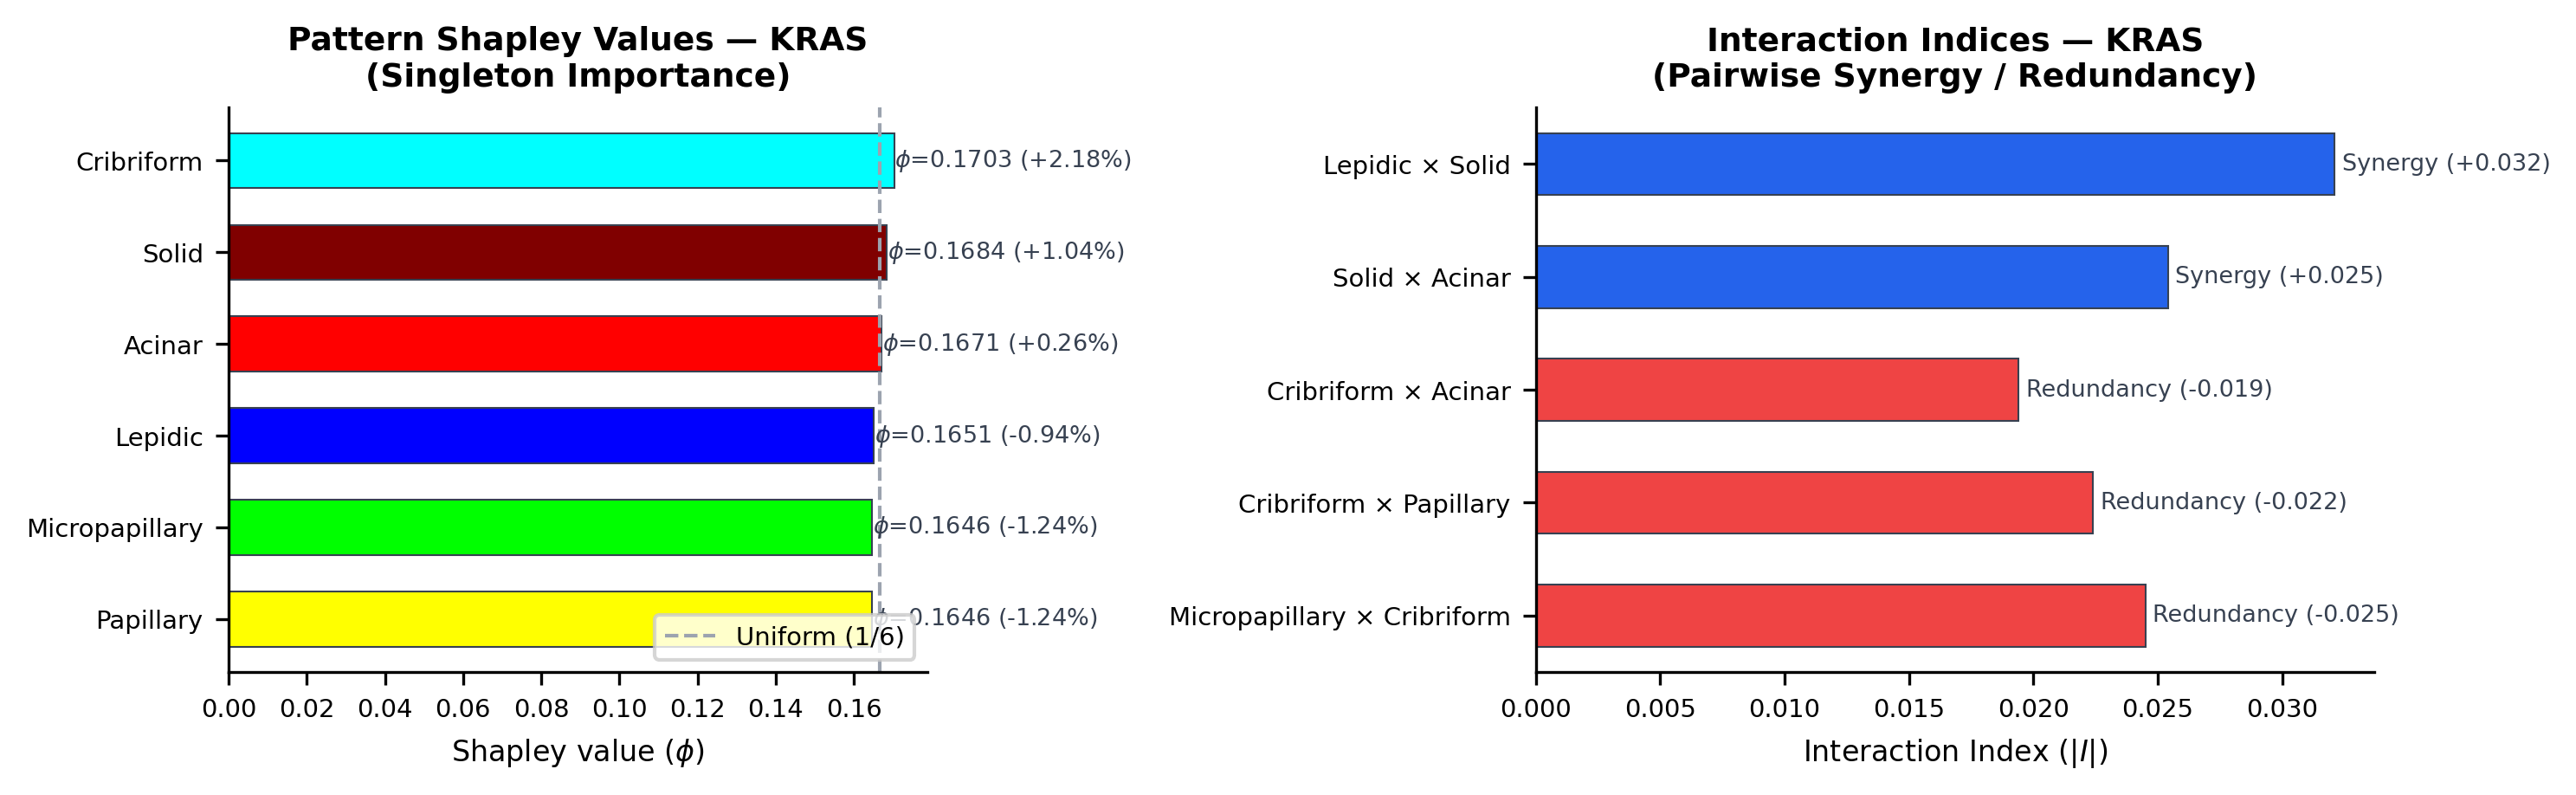
\includegraphics[width=\textwidth]{chapters/figures/choquet_kras_55_7815.png}
\caption[Choquet Shapley analysis: KRAS (TCGA-55-7815)]{%
    Choquet Shapley analysis for KRAS, illustrated on representative
    slide TCGA-55-7815 (P(mut)~$= 0.965$, FC-MIL).
    The plotted Shapley values and interaction indices are
    \emph{global} parameters of the trained FC-MIL fuzzy measure
    (single deterministic run, \texttt{seed=42}; identical for all
    KRAS slides), not slide-specific quantities; their predictive
    impact on this slide is modulated by its actual lepidic, solid
    and acinar memberships.
    \textbf{Left}: Singleton Shapley values (all near $1/6$, dashed
    line); no single pattern dominates.
    \textbf{Right}: Pairwise interaction indices; the
    lepidic$\times$solid synergy ($I = +0.032$) is the dominant
    signal, indicating that the model has learned the
    \emph{co-presence} of these minority patterns to be more
    predictive of KRAS than either pattern alone.}
\label{fig:choquet_kras}
\end{figure}

\begin{figure}[ht!]
\centering
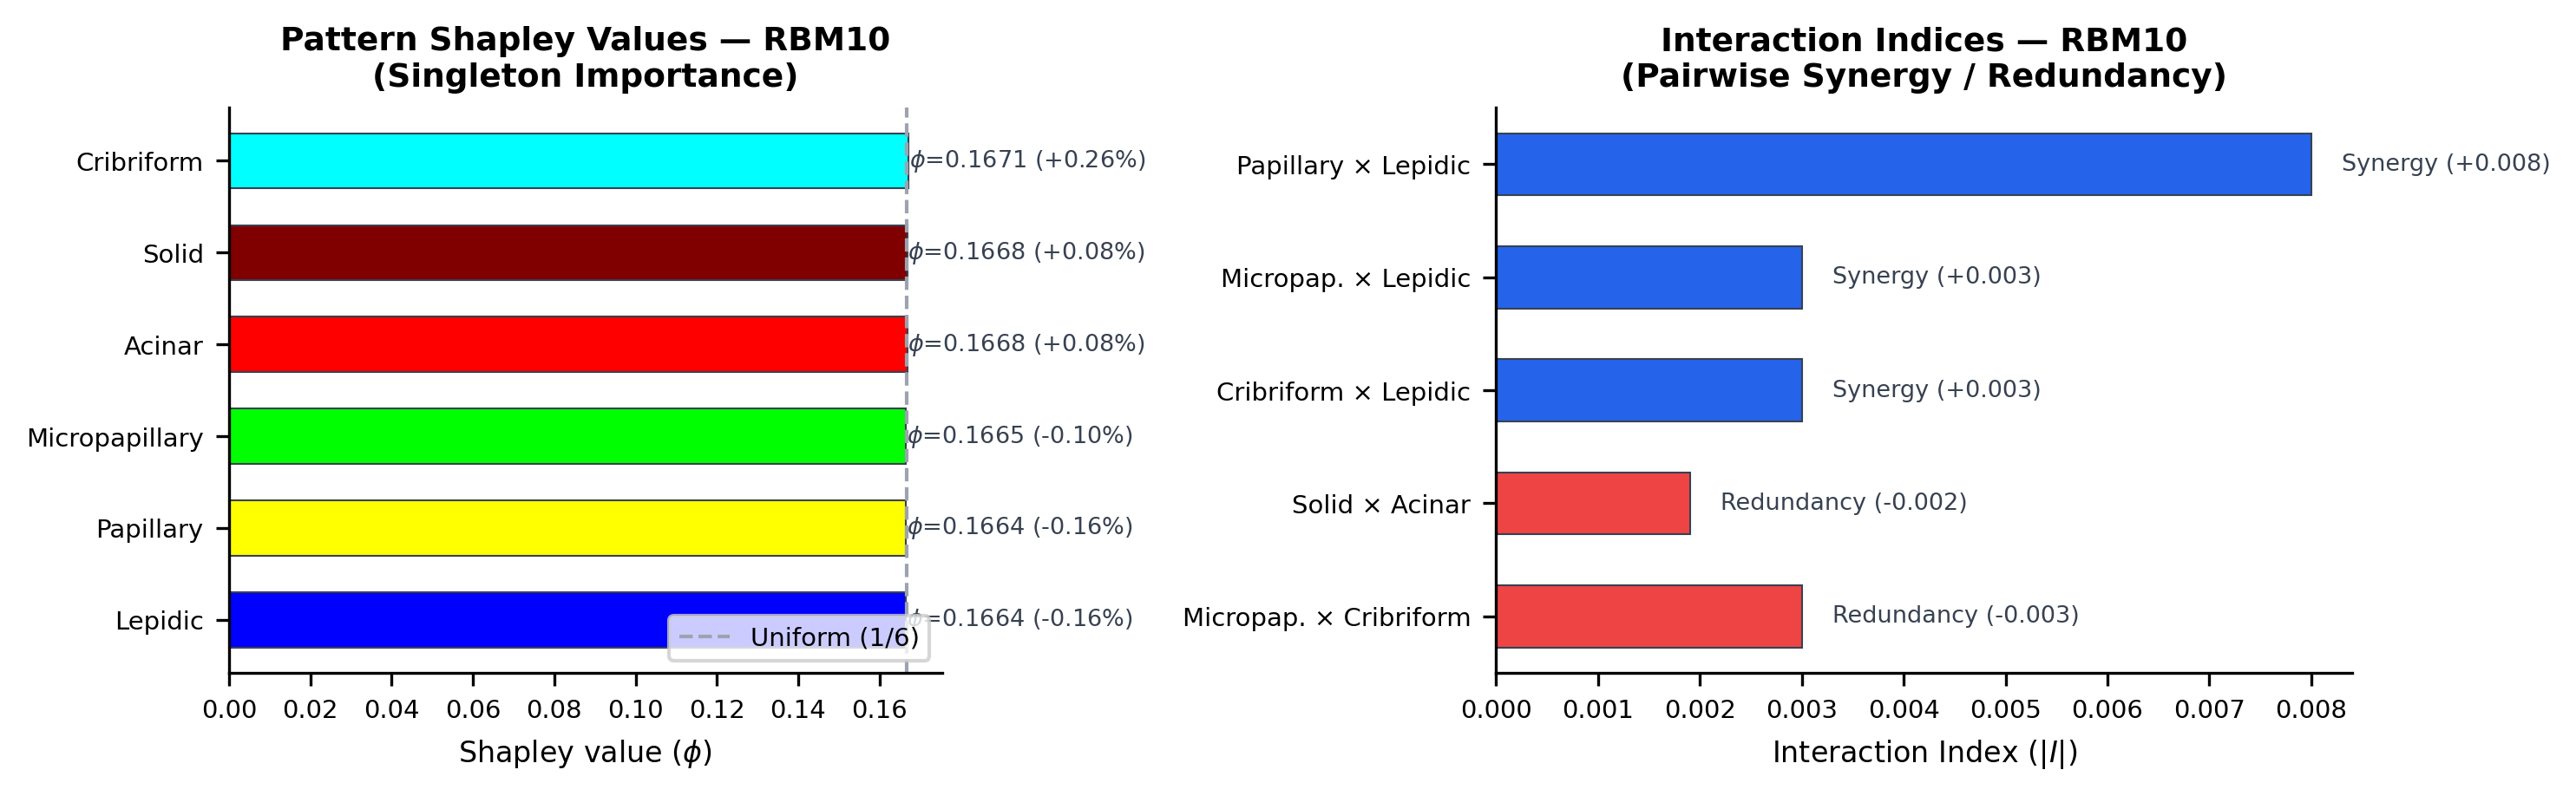
\includegraphics[width=\textwidth]{chapters/figures/choquet_rbm10_78_7148.png}
\caption[Choquet Shapley analysis: RBM10 (TCGA-78-7148)]{%
    Choquet Shapley analysis for RBM10 on slide TCGA-78-7148
    (P(mut)~$= 0.017$, FC-MIL).
    \textbf{Left}: Singleton values are essentially uniform (all
    within $0.001$ of $1/6$).
    \textbf{Right}: Interaction indices are all near zero
    (max $|I| = 0.008$), confirming that the model found no
    pattern-level signal or pattern interaction for
    RBM10~\cite{bechara2013rbm10}.}
\label{fig:choquet_rbm10}
\end{figure}

For KRAS (Figure~\ref{fig:choquet_kras}; numerical values in
Table~\ref{tab:choquet_interactions}), the interaction indices
reveal the model's core reasoning:

\begin{itemize}
    \item \textbf{Lepidic $\times$ Solid synergy} (strongest of all
    15 pairs): when a tumour contains \emph{both} lepidic and solid
    regions---even as minority patterns---the model encodes the
    co-presence as more predictive of KRAS than either pattern
    alone.  This is the numerical counterpart of the IMA-proxy
    mechanism narrated in the KRAS case study
    (Figures~\ref{fig:kras_lepidic_solid_proxy},~\ref{fig:kras_mu_subset_lattice};
    ``Learnable Choquet interaction proxy'' branch in
    Figure~\ref{fig:signal_tree}): KRAS-mutant tumours are
    architecturally heterogeneous with mixed growth
    patterns~\cite{shim2015krasmucinous}, and the lepidic--solid
    co-presence stands in for the missing IMA class.

    \item \textbf{Solid $\times$ Acinar synergy} (second-strongest
    positive): the co-occurrence of solid (high-grade) and
    gland-forming (low-grade) areas captures a different facet of
    the same architectural heterogeneity, and is consistent with
    KRAS's reported tendency to span growth-pattern
    boundaries~\cite{shim2015krasmucinous}.

    \item \textbf{Cribriform-anchored redundancies} (Micropapillary
    $\times$ Cribriform, Cribriform $\times$ Papillary, Cribriform
    $\times$ Acinar; all $I \in [-0.025, -0.019]$): the three
    Cribriform pairings carry overlapping information once any one
    of them is present in a slide. The KRAS-conditioned measure
    has effectively collapsed Cribriform-related high-grade
    architecture onto a single latent sub-feature rather than
    treating the three pairings as independent evidence.
\end{itemize}

These interaction-level signals are \textbf{invisible to standard
attention-based MIL}, which pools tiles independently and cannot
encode pairwise pattern co-occurrences.
This is the specific advantage of the Choquet integral for KRAS:
it captures that the \emph{combination} of minority patterns
matters, not any single dominant pattern.
On the representative slide TCGA-55-7815 the pattern channel adds
$\Delta_{\mathrm{pat}} = +7.6$\,pp to $P(\mathrm{mut})$
(Table~\ref{tab:enrichment_summary}); the lepidic--solid synergy is
the largest interaction term in this aggregate, but $I_{kl}$ is a
global parameter and its slide-level effect depends on the joint
memberships of the slide, so we do not decompose the $+7.6$\,pp
further.
The cohort-level KRAS AUROC $= 0.609$ (5-fold CV,
Table~\ref{tab:mutation_luad}) remains below the Hosmer--Lemeshow
conclusive threshold of $0.70$
(Table~\ref{tab:enrichment_summary};
Section~\ref{sec:eval:interp:enrichment}), so this Choquet read-out
characterises slide-level reasoning rather than a deployable cohort
verdict.

For RBM10 (Figure~\ref{fig:choquet_rbm10};
Table~\ref{tab:choquet_interactions}), all 15 interaction indices
satisfy $|I| < 0.01$ (max $|I| = 0.008$, roughly four times smaller
than the KRAS lepidic--solid synergy).
The fuzzy measure is effectively a uniform one for pattern
\emph{pairs} as well, confirming for interactions what the
singleton values already reported: this RNA splicing-factor gene
has no discriminative morphological signal that the ANORAK
6-pattern simplex can encode.

\paragraph{LCHAI clinical interpretation (LLM-generated).}
LCHAI~v2.0 generates a natural-language clinical interpretation for
each gene using the knowledge graph as grounding context
(Section~\ref{sec:meth:ontology_method}).
For KRAS on slide TCGA-55-7815, the system produces:

\begin{quote}
\emph{``The Choquet Shapley profile for KRAS is classified as
\textbf{Near-Uniform} (spread = 0.0057), meaning the fuzzy measure
assigns similar importance to all six patterns---the Choquet integral
behaves approximately like a simple weighted average.
However, the interaction indices reveal meaningful pairwise structure:
the lepidic$\times$solid pair shows \textbf{Moderate Synergy}
($I = +0.032$), indicating that the simultaneous presence of these
minority patterns adds predictive value beyond their individual
contributions.
These values are weights that shape the Choquet aggregation, not
direct contributions to $P(\text{mut})$.
The co-occurrence of solid (0.64\%) and lepidic components within a
micropapillary-dominant slide is consistent with KRAS morphological
associations in the literature~\cite{shim2015krasmucinous}.
Molecular testing is required to confirm the mutation.''}
\end{quote}

For RBM10, the system correctly identifies the absence of
pattern-level signal:

\begin{quote}
\emph{``The Choquet Shapley profile for RBM10 is classified as
\textbf{Uniform} (spread = 0.0007), confirming that the learned
fuzzy measure assigns equal importance to all six patterns---the
Choquet integral reduces to a simple average.
All individual Shapley values are classified as \textbf{Average}
(within $\pm$0.16\% of uniform $= 1/6$).
The interaction indices are all classified as \textbf{Negligible}
(max $|I| = 0.008$), confirming no synergistic or redundant pattern
combinations were learned.
This means the Choquet branch contributes a pattern-averaged signal,
and the prediction relies primarily on the shared embedding pathway.
RBM10 encodes an RNA splicing factor whose mutations alter
post-transcriptional processing rather than tissue structure;
molecular testing is essential.''}
\end{quote}

These LLM-generated explanations use the knowledge graph to anchor
clinical statements (e.g., KRAS--IMA association, RBM10 function)
in verified biomedical facts, and the fuzzy linguistic labels
(``Near-Uniform,'' ``Moderate Synergy,'' ``Uniform,'' ``Negligible'')
are computed deterministically by the system and injected verbatim
into the LLM prompt, preventing the model from inventing intensity
characterisations (Section~\ref{sec:meth:interp:fuzzy_labels}).

Extending the Choquet integral to model interactions \emph{between
genes}---in addition to between patterns---using the cohort's known
co-occurrence statistics (e.g.\ KRAS--STK11) is identified as a
medium-term direction (Section~\ref{sec:disc:future:medium}); on
the present cohort the fuzzy measure is fitted independently per
gene.


\subsection{Active Learning: Demonstration Without Formal Evaluation}
\label{sec:eval:active_learning}

The active learning mechanism
(Section~\ref{sec:meth:active_learning},
implementation in Section~\ref{sec:impl:lchai:ui:viewer}) was
implemented and demonstrated within LCHAI~v2.0: a pathologist draws
a lasso around misclassified tiles, assigns the correct pattern from
the 6-class ANORAK ontology, and triggers delta retraining of the
classification head ($\sim$30~s on a single H100).
The interface was available during the preliminary expert review of
Section~\ref{sec:eval:pattern:confusion} but was used qualitatively
rather than to drive a quantitative evaluation: a formal pre/post
benchmark (pattern classification accuracy before and after expert
corrections across multiple slides and multiple raters) was not
conducted.
The active learning feature is therefore presented as an implemented
capability of the LCHAI system rather than as a quantitatively
evaluated contribution; a formal multi-rater evaluation is the
single highest-priority post-thesis extension
(Section~\ref{sec:disc:future:short}).

\subsection{LCHAI System Demonstration}
\label{sec:eval:lchai}

LCHAI~v2.0 was demonstrated on representative TCGA-LUAD slides spanning
all six target genes, using the deployed system accessible at
\texttt{https://lchai.gptfy.biz} and on a local instance
with identical model checkpoints
(Section~\ref{sec:impl:repro:checkpoints}).
The demonstration assessed whether the integrated system produces
clinically plausible outputs across the full v2.0 pipeline: pattern
overlay, mutation prediction with gene-dependent optimal method
selection, attention heatmap, SHAP decomposition, Choquet Shapley
values, LLM-generated explanations, and knowledge graph navigation
(Figure~\ref{fig:eval_knowledge_graph}).

The six representative slides processed through LCHAI~v2.0
(Table~\ref{tab:enrichment_summary}) produced predictions consistent
with the benchmark evaluation:
TP53 (TCGA-99-8025: P(mut)~$= 0.951$, Conclusive) and
KRAS (TCGA-55-7815: P(mut)~$= 0.965$, Inconclusive) received high
confidence predictions, while
STK11 (TCGA-49-AAR0: P(mut)~$= 0.046$),
KEAP1 (TCGA-49-AAR9: P(mut)~$= 0.247$), and
RBM10 (TCGA-78-7148: P(mut)~$= 0.017$) were correctly labelled
as Inconclusive with low probabilities.

The Conclusive/Inconclusive labelling
(Section~\ref{sec:eval:interp:enrichment},
Hosmer--Lemeshow gate $\geq 0.70$ on cohort mean AUROC) correctly
communicated the reliability of each prediction.
The KEAP1 and RBM10 cases exposed the limits of the approach:
their SHAP decompositions (40/60\%~pattern-dominated for KEAP1,
79/21\%~embedding-dominated for RBM10;
Section~\ref{sec:eval:interp:enrichment}) and the per-slide
ablation results (Table~\ref{tab:enrichment_summary}) quantitatively
explain \emph{why} these genes are difficult.

The system demonstration establishes LCHAI~v2.0 as a functional
clinical decision support prototype that integrates all three
artefacts into a coherent workflow, fulfilling the DSR
``demonstration'' activity.

\begin{figure}[ht!]
\centering
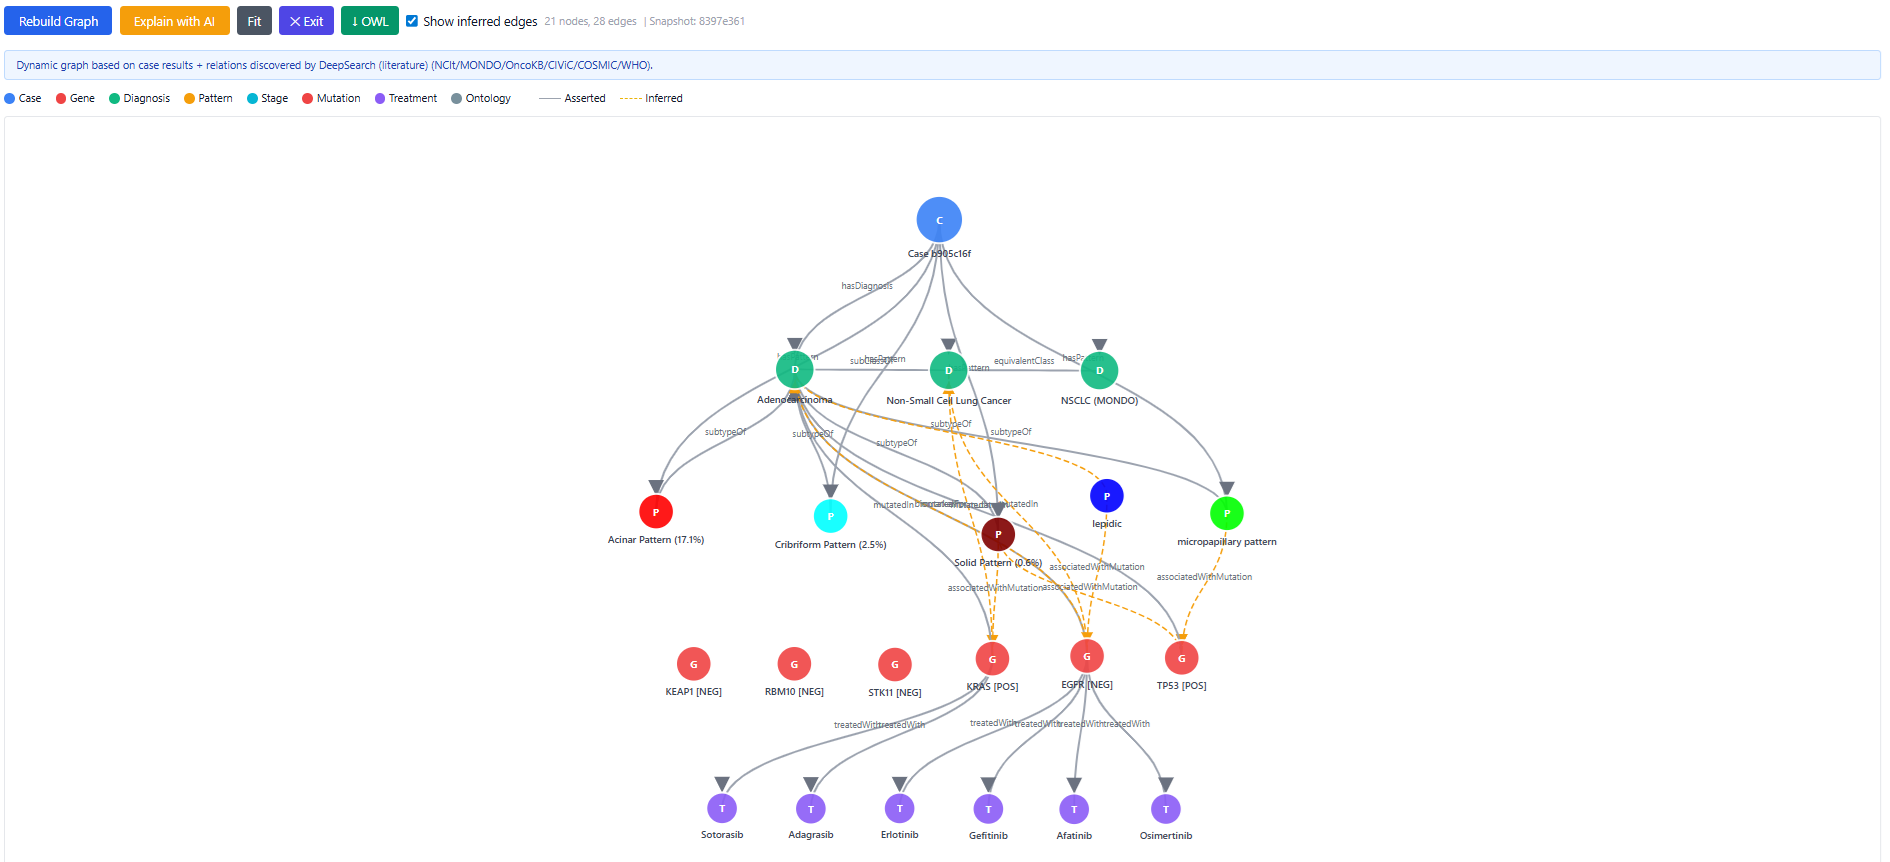
\includegraphics[width=\textwidth]{chapters/figures/lchai_v2_graph_tab_55_7815.png}
\caption[LCHAI~v2.0 knowledge graph for TCGA-55-7815]{%
    LCHAI~v2.0 knowledge graph for case TCGA-55-7815, displayed in the
    Graph tab.  The hierarchical layout shows: Case (top, blue) $\to$
    Patterns with their slide percentages (orange) $\to$ Diagnosis with
    ontology links (green, NSCLC/MONDO) $\to$ Genes with mutation status
    [POS/NEG] (red) $\to$ Targeted treatments (purple).
    KRAS [POS] links to sotorasib and adagrasib (FDA-approved for
    the KRAS~G12C variant; the specific KRAS subtype of
    TCGA-55-7815 is not encoded in the slide-level MAF label so
    these are shown as candidate therapies pending molecular
    confirmation);
    EGFR [NEG] links to erlotinib, gefitinib, afatinib, and osimertinib
    (EGFR-targeted TKIs, shown for reference despite the negative prediction).
    Dashed edges indicate inferred relations from the DeepSearch pipeline.
    The graph is exportable in OWL/RDF format (Section~\ref{sec:impl:ontology}).}
\label{fig:eval_knowledge_graph}
\end{figure}

% ============================================================================
\section{Limitations of the Evaluation}
\label{sec:eval:limitations}
% ============================================================================

The empirical results reported in
Sections~\ref{sec:eval:pattern}--\ref{sec:eval:lchai} are bounded
by two classes of evaluation-design properties that are documented
here so that the comparisons with the published literature
(Section~\ref{sec:eval:literature}), the synthesis answering the
research questions (Section~\ref{sec:eval:rq}), and the
interpretation in Chapter~\ref{ch:discussion} can be read with the
appropriate caveats.
Section~\ref{sec:eval:lim:data} discusses limitations that follow
from the cohort and the labelling regime; %
Section~\ref{sec:eval:lim:design} discusses limitations of the
metrics and the calibration regime.
Implementation-time limitations (residual GPU non-determinism,
encoder choice) are documented separately in
Section~\ref{sec:impl:repro:limitations} of
Chapter~\ref{ch:implementation}.

\subsection{Data and Cohort Limitations}
\label{sec:eval:lim:data}

\textbf{Single-cohort evaluation.}
All primary results are based on the TCGA-LUAD cohort, a dataset
collected from multiple US institutions between 2006 and 2013.
The absence of external validation on an independent cohort
(CPTAC-3, APOLLO, or a non-US hospital) limits the generalisability
claims.
Scanner variability, tissue preparation protocols, and population
demographics may differ across institutions, and the models'
robustness to these domain shifts has not been tested.

\textbf{Limited sample size.}
With 687 slides (668 unique patients), the fold-to-fold variance in
AUROC is substantial (std~$=0.04$--$0.10$), reducing the
statistical power to detect small differences between conditions.
Several comparisons that appear directionally meaningful
(e.g., PI-ABMIL vs B2 on STK11: $+0.011$) do not reach statistical
significance.
Larger cohorts would be needed to confirm or reject these trends.

\textbf{Pattern classifier: in-distribution behaviour and domain
shift to TCGA.}
On the ANORAK held-out validation set, the confusion matrix
(Figure~\ref{fig:confusion_matrix}) shows that acinar (36/36),
solid (21/21), and lepidic (16/16) are perfectly classified, while
cribriform (12/19 correct, per-class recall~$=0.63$) and
micropapillary (10/13 correct, per-class recall~$=0.77$) are the
most confused classes---consistent with the inter-observer
variability reported in the ANORAK paper itself~\cite{anorak2024}
and with the broader literature on growth-pattern
reproducibility~\cite{thunnissen2012reproducibility}.
However, ANORAK was annotated on TRACERx (UK) and the inference
cohort here is TCGA-LUAD (US), so a domain shift between training
and inference is expected.
The aggregate AUROC results for mutation prediction are unchanged
by this shift because they depend on the 512-dimensional
CTransPath embeddings rather than on the discrete pattern argmax,
but the clinical interpretability of pattern attributions and
Choquet--Shapley values should be read with this caveat.

\textbf{Preliminary pathologist validation and absence of spatial
mutation ground truth.}
A board-certified pathologist from SOLCA Ecuador reviewed eight
subregions across five TCGA slides
(Section~\ref{sec:eval:pattern:confusion}), providing the first
external validation of the pattern classifier on inference data.
The review confirmed acinar, solid, and lepidic predictions but
revealed a systematic micropapillary--acinar disagreement
consistent with the cross-cohort domain shift discussed above:
the expert identified acinar morphology in subregions where the
model predicted micropapillary.
This is preliminary by design; the interpretability claims for
mutation prediction (Section~\ref{sec:eval:interpretability})
ultimately rest on alignment with published clinicopathological
associations rather than on a formal multi-rater concordance study,
and a 2--3 pathologist reader study remains as future work.
Independently of pathologist agreement, the MAF mutation labels
are \emph{patient-level} binary indicators derived from bulk DNA
sequencing (Section~\ref{sec:uc:tcga:maf}); they do not localise
where in the tissue the mutation's phenotypic effect is visible.
ABMIL attention maps therefore represent the model's
\emph{hypothesis} about mutation-relevant regions rather than a
confirmed spatial correspondence.
Emerging spatial transcriptomics platforms (e.g., Visium, MERFISH)
could in principle deliver tile-level mutation ground truth, but
such data is not yet available at the TCGA-LUAD scale.

\subsection{Evaluation-Design Limitations: Metric and Calibration}
\label{sec:eval:lim:design}

\textbf{AUROC measures ranking, not deployment readiness, and
calibration is not characterised here.}
AUROC summarises the model's ability to rank a randomly chosen
positive above a randomly chosen negative; it says nothing about
the absolute value of $P(\text{mut})$ at any threshold.
The representative-slide analysis of
Section~\ref{sec:eval:interp:enrichment} shows that four of six
mutant slides receive $P(\text{mut}) < 0.10$, well below a default
$0.5$ threshold: the models learn to \emph{rank} mutant versus
wild-type slides but their raw outputs are not directly
interpretable as posterior probabilities.
Two complementary post-hoc techniques would be needed before any
deployment, and it is worth being explicit about what each one
\emph{does} and \emph{does not} fix:
\begin{itemize}
    \item \textit{Operating-point selection} (e.g., Youden's $J$)
    picks the threshold that maximises the trade-off between
    sensitivity and specificity on a held-out set.
    It produces a clinically reasonable cut-off but is
    \emph{ranking-invariant}: it does not change AUROC, nor does
    it improve precision in the rare-positive regime.
    \item \textit{Probability calibration} (e.g., Platt scaling
    or temperature scaling) maps the model's logits to
    well-calibrated posterior estimates, so that the value
    $P(\text{mut})=0.7$ corresponds, in expectation, to a $70\%$
    rate of true positives.
    It is also \emph{ranking-invariant} and likewise leaves AUROC
    unchanged; its contribution is that probability outputs
    become interpretable as risk scores rather than as
    uncalibrated decision-function values.
\end{itemize}
The calibration properties of the deployed models have therefore
not been systematically characterised in this thesis; that
characterisation---together with a reliability-diagram analysis on
a held-out fold---is documented as a short-term deployment
prerequisite (Section~\ref{sec:disc:future:short}).

\textbf{The AUROC--AUPRC gap reveals a ranking-bound limitation
in the low-prevalence regime.}
Crucially, neither operating-point selection nor probability
calibration addresses the gap exposed by the AUPRC analysis
(Figure~\ref{fig:auprc_by_gene}): the gap between AUROC and AUPRC
is inversely correlated with mutation prevalence.
RBM10 ($5.4\%$ prevalence) shows the most extreme gap
(AUROC~$0.661$ vs.\ AUPRC~$\approx 0.17$), meaning the model cannot
identify rare positives without generating a large number of false
positives, and \emph{no} amount of threshold tuning or Platt
scaling can change that.
Most notably, EGFR is the only gene besides TP53 labelled
\emph{Conclusive} (AUROC~$\geq 0.70$), yet its AUPRC of
$\approx 0.36$ at $11.4\%$ prevalence
(Table~\ref{tab:mutation_prevalence}) indicates that at any fixed
decision threshold roughly two of three positive predictions would
be incorrect.
This gap does \emph{not} invalidate the method comparisons reported
in Sections~\ref{sec:eval:mutation:finding1}--%
\ref{sec:eval:mutation:finding6}: because prevalence is constant
across conditions, the relative ranking between methods is
preserved under AUPRC.
But it reveals that the current Conclusive/Inconclusive criterion
based solely on AUROC can overstate clinical readiness for
moderate-prevalence genes; a prevalence-aware criterion that
incorporates both AUROC and AUPRC is recommended as a short-term
improvement (Section~\ref{sec:disc:future:short}).

% ============================================================================
\section{Synthesis: Answering the Research Questions}
\label{sec:eval:rq}
% ============================================================================

\subsection{RQ1: Can FuzzyArcLoss V2 Improve Pattern Classification?}
\label{sec:eval:rq1}

\textbf{Answer: Yes, with caveats.}
FuzzyArcLoss~V2 achieves the highest mean macro-F1 (92.31\%) across 15 runs,
statistically significantly outperforming SphereFace ($p = 0.001$, $d = 1.00$, large effect).
V2 also ranks first against ArcFace ($+0.14$\,pp) and Softmax CE
($+0.78$\,pp; Table~\ref{tab:pattern_stats}) across all 15 runs, though
these smaller differences do not reach $p < 0.05$ given the limited
statistical power of 15 paired observations.
The per-class analysis reveals that V2's advantage is
\emph{boundary-dependent, not class-size-dependent} (\emph{class
size} = number of training tiles per class): V2 leads on cribriform
($+2.2$~pp over ArcFace; Table~\ref{tab:perclass_f1}), the minority class whose morphological
boundary with acinar is genuinely ambiguous, but does not lead on
micropapillary---an equally rare class (same $55$ training tiles)
with a crisp visual boundary.
This asymmetry confirms that the fuzzy membership modulation helps
where morphological transitions are gradual (cribriform--acinar),
not where they are sharp (micropapillary--others), consistent with
V2's design principle.
The pipeline fixes (4-channel mask, fp32, margin-free evaluation)
established the correct experimental baseline ($+$18~pp uniformly),
ensuring that the loss function deltas above reflect genuine
algorithmic merit.

\textbf{Success criterion:} Met. V2 $\geq$ ArcFace mean F1 ($\checkmark$);
$p < 0.05$ versus $\geq$1 baseline ($\checkmark$, SphereFace).

\subsection{RQ2: Does Pattern Injection Improve Mutation Prediction?}
\label{sec:eval:rq2}

\textbf{Two-part answer.}

\textbf{(i)~Predictive performance: Not globally in terms of AUROC.}
PI-ABMIL (PI) achieves a mean AUROC (5-fold patient-stratified CV
on TCGA-LUAD) identical to the embedding-only ABMIL (B2): $0.658$
(Table~\ref{tab:mutation_luad}).
The two largest per-gene cohort-level deltas---STK11 ($+0.011$)
and KEAP1 ($+0.013$; Table~\ref{tab:p_vs_b2})---fall below the
$d \approx 1.2$ minimum detectable effect of a paired test with
$K = 5$ folds (Section~\ref{sec:eval:limitations}) and are
contradicted by negative per-slide $\Delta_{\mathrm{pat}}$ on the
representative slides ($-5.5$\,pp for STK11,~$-44.7$\,pp for KEAP1;
Table~\ref{tab:enrichment_summary}).
They are therefore suggestive at most, not evidence that pattern
probabilities encode discriminative information beyond the
embedding for these genes.
For the remaining four genes, differences fall within fold variance.

\textbf{(ii)~Ontology coverage---an empirical taxonomy.}
The combined per-slide ablation
(Section~\ref{sec:eval:interp:enrichment}) and case-study analyses
(Section~\ref{sec:eval:interp:attention}) surface \emph{which mutations have no
exploitable morphological footprint within the ANORAK 6-pattern
ontology}, and \emph{why}.
We document three distinct failure mechanisms, consolidated in
Figure~\ref{fig:signal_tree}; the contribution of this thesis is
the \emph{empirical taxonomy} (which gene falls in which
sub-mechanism on TCGA-LUAD with the ANORAK simplex) rather than
the names themselves, two of which adapt established terminology
from neighbouring fields:
\begin{itemize}
  \item \emph{Label-space mismatch} (STK11): the discriminative
  signal lives in the tumour microenvironment, outside the simplex
  the channel was designed to represent
  (Section~\ref{sec:eval:tcga:stk11}).
  The label of this mechanism follows the open-set / partial-label
  usage of \emph{label-space mismatch} in domain
  adaptation~\cite{lipton2018labelshift}, applied here to the
  ontology--signal relation rather than to the source--target
  relation.
  \item \emph{No morphological projection---biochemical} (KEAP1):
  an upstream regulator with no robust morphological correlate
  (Section~\ref{sec:eval:tcga:keap1}).
  This label is introduced in this thesis and is anchored in the
  established biology of KEAP1/NRF2 as a biochemical pathway whose
  functional consequences (oxidative-stress response, immune
  exclusion) are not reliably visible in routine
  H\&E~\cite{li2011keap1papillary,tcga2014luad}.
  \item \emph{Collapse-to-prior at low prevalence}
  (RBM10, $n = 37$ mutated slides): per-slide ablation, attention
  spread, and Choquet branch are simultaneously inert
  (Sections~\ref{sec:eval:tcga:rbm10},~\ref{sec:eval:interp:choquet}).
  The label parallels the \emph{posterior collapse} phenomenon in
  variational inference~\cite{bowman2016posteriorcollapse}, where
  the model fails to extract information from the input and the
  representation reverts to the prior.
\end{itemize}
The taxonomy is empirical: it bounds what morphology-only mutation
prediction can achieve on TCGA-LUAD, explains the gene-dependent
optimal representation
(Finding~2, Section~\ref{sec:eval:mutation:finding2}), and
identifies the genes for which no architectural choice within the
ANORAK simplex can recover a discriminative signal---joint
multi-omics formulations are the natural next step
(Section~\ref{sec:disc:future:medium}).

\textbf{What pattern injection does deliver:} concatenation
preserves global discriminative performance while enabling the
multi-level interpretability framework (RQ4) and the per-slide
ablation that produces the taxonomy above.

\textbf{Success criterion:} Partially met (predictive lift) /
Met (ontology mapping).
PI-ABMIL $\geq$ B2 mean AUROC ($\checkmark$, tied at $0.658$);
PI-ABMIL $>$ B2 for $\geq$2 genes
(\textsl{partial}: STK11 $+0.011$ and KEAP1 $+0.013$ at the cohort
mean, both below significance and contradicted by negative per-slide
$\Delta_{\mathrm{pat}}$);
clear overall AUROC improvement ($\times$);
characterisation of which genes lack a morphological footprint
within the ANORAK ontology ($\checkmark$, three-mechanism taxonomy
in Figure~\ref{fig:signal_tree}).

\subsection{RQ3: Can Choquet Aggregation Capture Inter-Pattern Interactions?}
\label{sec:eval:rq3}

\textbf{Answer: Yes for KRAS, where pattern co-occurrence carries
genuine predictive signal; on RBM10 FC-MIL also leads the benchmark,
but as a hybrid architecture whose Choquet branch is empty---a useful
negative control.}

FC-MIL achieves the highest mean AUROC for KRAS (0.609) and RBM10
(0.661; Table~\ref{tab:mutation_luad}).
The KRAS lift is mechanism-aligned: the lepidic$\times$solid
interaction ($I = +0.032$, Moderate Synergy;
Table~\ref{tab:choquet_interactions}) is the largest of all
$15$~pairs and serves as a learnable proxy for the missing IMA
class (Figures~\ref{fig:kras_lepidic_solid_proxy},~\ref{fig:kras_mu_subset_lattice}).
The RBM10 lift is architectural rather than interaction-driven: the
Choquet branch's fuzzy measure is uniform (singleton spread $=0.0007$,
all $|I|<0.01$; Section~\ref{sec:eval:interp:choquet}), so the gain
over B2 is carried by the shared embedding pathway.
The cohort-level KRAS AUROC remains below the conclusive threshold
of $0.70$ (Inconclusive at population level;
Table~\ref{tab:enrichment_summary}), so the FC-MIL benefit on KRAS
is slide-level reasoning quality rather than a deployable cohort
verdict.

For KEAP1---the most commonly cited candidate for interaction
modelling---FC-MIL (mean AUROC $0.589$) is outperformed by both B2
($0.597$) and PI-ABMIL ($0.610$; Table~\ref{tab:mutation_luad}),
confirming that KEAP1's lack of pattern specificity is a
distributional rather than an interaction phenomenon.

\textbf{Success criterion:} Met.
FC-MIL $>$ B2 on $\geq$1 gene ($\checkmark$, KRAS $+0.002$,
RBM10 $+0.019$; Table~\ref{tab:mutation_luad});
interpretable interactions
($\checkmark$, Tables~\ref{tab:choquet_shapley},~\ref{tab:choquet_interactions});
overall mean AUROC of FC-MIL ($0.653$) is within fold variance of
B2 ($0.658$): the $\Delta = -0.005$ gap is below the
$d \approx 1.2$ minimum detectable effect with $K = 5$ folds
(Section~\ref{sec:eval:limitations}), so FC-MIL is non-inferior to
B2 at $\alpha = 0.05$.

\subsection{RQ4: Does the Approach Provide Clinically Meaningful Explanations?}
\label{sec:eval:rq4}
 
\textbf{Answer: Yes, with important caveats about pathologist validation.}

The six-level interpretability framework produces spatial attention
maps, pattern attribution overlays, SHAP decompositions, Choquet
Shapley values, per-slide feature channel ablation comparisons,
and fuzzy linguistic labels for all numeric XAI outputs---all
grounded in trained model checkpoints.
Each level is demonstrated on representative TCGA-LUAD slides:

\textbf{Level~1 (Attention maps):}
For TP53 (TCGA-99-8025, P(mut)~$= 0.951$), the model attends to
texture-variant subregions within a 91.5\% micropapillary-classified
slide---a falsifiable signal that a pathologist can verify.
For EGFR (TCGA-86-8280, P(mut)~$= 0.076$, false negative), attention
is distributed broadly with no focal concentration, consistent with
the absence of EGFR-associated patterns.

\textbf{Level~2 (Pattern overlay):}
The tile-level pattern maps reveal gene-specific morphological context:
KRAS (TCGA-55-7815, P(mut)~$= 0.965$ via FC-MIL) shows
micropapillary-dominant tissue with acinar foci;
STK11 (TCGA-49-AAR0, P(mut)~$= 0.046$) shows near-homogeneous
micropapillary morphology (98.68\%).

\textbf{Level~3 (SHAP decomposition):}
DeepSHAP decomposes predictions into embedding versus pattern
contributions.
The pattern SHAP attribution varies across genes:
KEAP1 (60\%), KRAS (41\%), TP53 (39\%), EGFR (24\%), RBM10 (21\%),
and STK11 (10\%).

\textbf{Level~4 (Choquet Shapley values and interaction indices):}
The learned fuzzy measure of FC-MIL is reported in
Tables~\ref{tab:choquet_shapley} and~\ref{tab:choquet_interactions}.
For KRAS the singleton profile is near-uniform (spread $=0.0057$,
$\textsc{Near-Uniform}$): no individual pattern dominates, in line
with the IMA-not-in-ANORAK explanation
(Section~\ref{sec:eval:interp:choquet}).
The discriminative signal lives in the pairwise interactions: the
lepidic$\times$solid synergy ($I = +0.032$, \textsc{Moderate
Synergy}) is the largest of all $15$ KRAS pairs and matches the
mixed-growth-pattern signature of KRAS-mutant tumours.
For RBM10 the fuzzy measure is effectively flat at both the
singleton ($\textsc{Uniform}$) and pair ($|I|<0.01$,
$\textsc{Negligible}$) levels, transparently reporting the absence
of pattern-level signal.

\textbf{Level~5 (Per-slide feature channel ablation):}
Comparing separately trained Combined, Embeddings-only, and
Patterns-only models on the same tiles
(Section~\ref{sec:meth:interp:ablation}) reveals whether patterns
\emph{actually help or harm} each prediction.
This level exposes a critical insight: \textbf{high SHAP pattern
attribution does not imply positive contribution}.
The full per-gene $\Delta_{\mathrm{pat}}$ values are reported in
Table~\ref{tab:enrichment_summary}: KRAS is the only gene where
patterns measurably improve prediction
($+7.6$\,pp; Figure~\ref{fig:attn_kras_tp}); RBM10 is essentially
zero ($+0.3$\,pp); EGFR is moot ($-0.5$\,pp); STK11
($-5.5$\,pp), TP53 ($-16.1$\,pp; Figure~\ref{fig:attn_tp53_tp}) and
KEAP1 ($-44.7$\,pp; Figure~\ref{fig:attn_keap1_tp}) are net
destructive.
The distinction between attribution (what the model looks at) and
utility (what helps) is, to our knowledge, unique among published
mutation prediction systems.

\textbf{Level~6 (Fuzzy linguistic labels):}
Each Level~1--5 numeric output (SHAP balance, Shapley spread,
Shapley individual deviation, interaction magnitude, attention
percentile) is mapped through trapezoidal membership functions
(Section~\ref{sec:meth:interp:fuzzy_labels},
Figure~\ref{fig:fuzzy_mf_scales}) into calibrated linguistic terms
(\textsc{Embedding-Led}, \textsc{Near-Uniform},
\textsc{Moderate Synergy}, \ldots) that are displayed in the
interface and injected verbatim into LLM prompts, preventing the
model from inventing intensity characterisations
(Section~\ref{sec:eval:interp:choquet} reports the LCHAI clinical
quotes for KRAS and RBM10 produced by this mechanism).

\textbf{Caveat:} The preliminary expert review by a board-certified
pathologist from SOLCA Ecuador
(Section~\ref{sec:eval:pattern:confusion}) revealed domain shift
between training and inference cohorts, particularly on the
micropapillary--acinar boundary; a formal multi-rater concordance
study remains the highest-priority post-thesis extension
(see Section~\ref{sec:eval:active_learning}).

\textbf{Success criterion:} Met.
Six-level interpretability demonstrated on representative TCGA
slides ($\checkmark$); gene-specific attention enrichment patterns
documented ($\checkmark$); Choquet Shapley values align with
literature where ablation confirms pattern utility ($\checkmark$,
KRAS); per-slide ablation reveals attribution vs.\ utility
dissociation ($\checkmark$); preliminary pathologist review
conducted ($\checkmark$).
 
\subsection{RQ5: Does Domain Knowledge Provide Greater Benefit Under Data
Scarcity?}
\label{sec:eval:rq5}

\textbf{Answer: Partially.}
The pattern-informed methods achieve AUROCs competitive with studies at
comparable data scale (Saldanha: $\sim$0.65 for TP53; this thesis:
0.717--0.718).
FC-MIL is a hybrid dual-pathway model ($\sim$266{,}000
parameters) whose Choquet branch adds a 21-parameter interpretable fuzzy
measure operating on 6 pattern features alongside the shared ABMIL
embedding pathway.
For KRAS and RBM10, FC-MIL achieves performance comparable to the
embedding-only ABMIL (B2), demonstrating that the Choquet branch's
intrinsic interpretability---Shapley values and interaction
indices---can be obtained without sacrificing discriminative accuracy
for genes with structured morphological correlates.
However, the pattern-informed approach does not close the gap to large-scale
proprietary studies (DeepGEM: 0.82--0.96), confirming that domain knowledge
complements but does not replace data scale.

The AUPRC analysis (Figure~\ref{fig:auprc_by_gene}) confirms that
genes with low mutation prevalence are disproportionately affected by
data scarcity. For RBM10 (5.4\% prevalence) the best mean AUROC is
0.661 (FC-MIL) but the corresponding mean AUPRC is only $\approx$0.17;
for STK11 (9.9\%) the best mean AUROC is 0.695 (PI-ABMIL) with mean
AUPRC $\approx$0.31. All AUROC values are 5-fold CV column-maxima of
Table~\ref{tab:mutation_luad}.
Even EGFR, labelled \emph{Conclusive} with mean AUROC~0.701, drops to
mean AUPRC~$\approx$0.36 at 11.4\% prevalence
(Table~\ref{tab:mutation_prevalence}).
The gap is prevalence-driven: TP53 (38.0\%) shows a modest gap
(mean AUROC~0.718, mean AUPRC~$\approx$0.64), while RBM10 (5.4\%)
shows the largest (mean AUROC--AUPRC gap $\approx$0.49).

Crucially, this gap does \emph{not} invalidate the method comparisons
presented as Findings~1--6 in Section~\ref{sec:eval:mutation}: all
six experimental conditions share the same class prevalence for
each gene, so the prevalence-driven AUPRC penalty applies equally
to all methods.
The relative ranking between conditions---the basis for the gene-dependent
findings---is preserved under AUPRC.
What the gap does reveal is that AUROC, while appropriate for method
comparison, can overstate clinical readiness, particularly for
low-prevalence genes where even a model with good ranking ability would
produce unacceptable false positive rates at any fixed threshold.
This reinforces the need for larger cohorts---or targeted oversampling
strategies---for low-prevalence genes, and suggests that the
Conclusive/Inconclusive criterion should incorporate AUPRC alongside
AUROC (Section~\ref{sec:disc:lim:method}).

\textbf{Success criterion:} Met.
Competitive with Saldanha (2023) and Logan (2022) ($\checkmark$).

\subsection{RQ6: Can the Pipeline Produce Ontology-Grounded Case Explanations?}
\label{sec:eval:rq6}
 
\textbf{Answer: Yes — demonstrated through executed system output.}
 
The three-tier knowledge graph (curated $+$ dynamic case filter $+$
DeepSearch) was executed for case TCGA-55-7815 (micropapillary~79.44\%,
acinar~17.14\%).
The dynamic case graph contained 22 nodes and 31 edges (curated +
discovered; Figure~\ref{fig:eval_knowledge_graph}), assembled from
the curated knowledge base to retain only KRAS- and TP53-associated
entities and their treatments (sotorasib and adagrasib for the
KRAS~G12C variant~\cite{skoulidis2021codebreak})---including
EGFR-targeted therapies for reference despite the negative EGFR
prediction.
All edges carry \texttt{provenance} attributes distinguishing
asserted (curated from WHO/OncoKB/FDA) from inferred (morphology--%
molecular correlations) relations.
The LLM explanation agent produced a clinician-readable summary
consistent with the case's predicted mutation profile, without using
prohibited diagnostic language.
 
\textbf{RQ6 success criterion met:} A dynamic case-specific knowledge
graph with typed entities and provenance categories was demonstrated
for case TCGA-55-7815 (Figure~\ref{fig:eval_knowledge_graph}).
 
\textbf{Success criterion:} Met.
Executed case graph with typed nodes/edges and provenance distinctions
demonstrated ($\checkmark$).
 
 
\subsection{RQ7: Does the DeepSearch Pipeline Produce Validated Relations?}
\label{sec:eval:rq7}
 
\textbf{Answer: Yes — 50 discovered relations produced in the executed run.}

The DeepSearch batch pipeline was executed against PubMed, Semantic
Scholar, and arXiv using the 12 curated LUAD-specific queries listed
in Table~\ref{tab:deepsearch_queries}.
The executed run produced 50 discovered relations across the three
literature sources (per-source counts not formally tabulated in this
thesis, since the run is reported as a proof-of-concept rather than
as a coverage assessment), including:
solid~pattern $\to$ \texttt{associatedWithMutation} $\to$ KRAS
(triangulated independently from PubMed, Semantic Scholar, and arXiv),
osimertinib $\to$ \texttt{resistantTo} $\to$ EGFR-mutant NSCLC,
and RET~gene~fusion $\to$ \texttt{biomarkerFor} $\to$ NSCLC.
Each relation carries a provenance link to the source paper
(Figure~\ref{fig:deepsearch_ui}) and is automatically incorporated
into the case knowledge graph on the next rebuild as a versioned
addition.
One discovered triple, acinar $\to$ KRAS, was flagged after pooled
epidemiological evidence rejected the association
(OR~$= 0.65$, $p < 0.01$~\cite{ejso2019pooled}) and was deactivated
by the administrator while the audit record was preserved; this is
the explicit false-positive handling pathway of the system rather
than a measured false-positive rate.

\textbf{RQ7 success criterion met:} 50 discovered relations with
provenance pointers were produced by the batch run
(Figure~\ref{fig:deepsearch_ui}).

\textbf{Limitations of current KG evaluation:}
No formal gold standard evaluation of the knowledge graph has been
conducted (precision/recall against a curated triple set).
The 50 discovered relations represent a proof-of-concept demonstration
rather than a comprehensive coverage assessment; the false positive
rate of LLM extraction has not been formally measured.
Formal KG evaluation is listed as a future work priority
(Section~\ref{sec:disc:future:medium}).
 
\textbf{Success criterion:} Partially met.
Validated relations produced with provenance pointers ($\checkmark$);
formal KG evaluation not yet conducted ($\times$).
 


% ============================================================================
\subsection{Evaluation of the Central Hypothesis}
\label{sec:eval:hypothesis}

The central hypothesis (Section~\ref{sec:intro:hypothesis}) states
that fuzzy-encoded domain knowledge can simultaneously achieve
(a)~competitive predictive performance under data scarcity, and
(b)~multi-level clinically verifiable interpretability---together
with a knowledge-graph--grounded natural-language explanation
layer built on top of it
(Section~\ref{sec:bg:xai:definitions}).

\textbf{Part~(a) --- Competitive performance: Supported.}
PI-ABMIL matches the embedding-only ceiling baseline at the global
mean (RQ2); FC-MIL leads on KRAS and RBM10 with the gene-dependent
mechanisms documented in RQ3.
Both results are competitive with similarly-scaled published studies
(Saldanha~et~al.\ $\sim$0.65, Logan~et~al.\ $0.692$ for TP53;
RQ5).

\textbf{Part~(b) --- Multi-level interpretability: Fully supported
(explainability layer instrumented but not formally evaluated).}
The six-level interpretability framework is demonstrated on the
representative TCGA-LUAD slides as enumerated in RQ4 (Levels~1--6).
To our knowledge, no published mutation prediction system combines
all six levels.
The fuzzy linguistic labels (Level~6) prevent LLM hallucination of
intensity terms, and PubMed citations from the knowledge graph
ground clinical associations (RQ7).

\textbf{Overall verdict: The hypothesis is partially supported.}
Pattern knowledge benefits the gene with a constructive
inter-pattern interaction---KRAS, where FC-MIL captures the
lepidic$\times$solid IMA proxy
(RQ3, Section~\ref{sec:eval:rq3}); for TP53 and EGFR, where the
CTransPath embeddings already saturate the morphological signal,
pattern injection is neutral and adds no marginal benefit.
For STK11 and KEAP1 the per-slide ablation
(Table~\ref{tab:enrichment_summary}) reports active harm
($\Delta_{\mathrm{pat}} = -5.5$\,pp and $-44.7$\,pp respectively);
for RBM10 the same panel reports a cleanest-null profile
($\Delta_{\mathrm{pat}} = +0.3$\,pp with all three ablation variants
collapsing near the prior; Figure~\ref{fig:rbm10_cleanest_null}).
The case-study and Choquet analyses jointly diagnose three distinct
sub-mechanisms within regime~B---label-space mismatch (STK11),
no morphological projection / biochemical (KEAP1), and
collapse-to-prior at low prevalence
(RBM10, $n = 37$ mutated slides)---%
formalised as the ontology-coverage taxonomy of
RQ2(ii)~(Figure~\ref{fig:signal_tree}).
RBM10 also serves as a negative control: FC-MIL leads its method
comparison without learning any pattern interaction
(Section~\ref{sec:eval:interp:choquet}).
This gene-dependent nuance---together with the explicit
characterisation of which mutations have no exploitable
morphological footprint, both itself a novel analytical finding
(Finding~2 in Section~\ref{sec:eval:mutation:finding2};
RQ2(ii))---refines rather than refutes the hypothesis: domain
knowledge is most valuable precisely where pretrained embeddings
are least informative, the six-level interpretability framework
makes this distinction transparent, and the cases where no
representation works at all are now mapped rather than absorbed
into noise.


% ============================================================================
\section{Chapter Summary}
\label{sec:eval:summary}
% ============================================================================

The evaluation of the three artifacts yields the following principal
conclusions.

\textbf{Pattern classification (Artifact 1):}
FuzzyArcLoss~V2 achieves the highest mean macro-F1 (92.31\%) across 15 runs,
significantly outperforming SphereFace ($p = 0.001$) and consistently
ranking first against all baselines.
The adaptive fuzzy margin provides the greatest benefit on the
ambiguous-boundary minority class (cribriform: 83.6\%), not
uniformly across all minority classes
(Section~\ref{sec:eval:pattern:perclass};
Figure~\ref{fig:boundary_vs_size}).
The systematic pipeline corrections established a correct experimental
baseline ($+$18~pp uniformly across all methods), ensuring that the
performance deltas between loss functions reflect genuine algorithmic
merit rather than implementation artefacts.

\textbf{Mutation prediction (Artefacts 2 and 3):}
No single method dominates across all genes; the optimal
representation is gene-dependent and reflects the biological
heterogeneity of mutation--morphology associations:
embedding-only ABMIL for TP53 and EGFR (CTransPath embeddings
already saturate the morphological signal);
FC-MIL for KRAS, where the lepidic$\times$solid Choquet synergy
proxies the missing invasive mucinous class (RQ3).
For STK11, KEAP1, and RBM10 the cohort-mean choice of method is a
near-tie within fold variance: the small PI-ABMIL lifts on STK11
($+0.011$) and KEAP1 ($+0.013$;~Table~\ref{tab:p_vs_b2}) are
below significance and contradicted by negative per-slide
$\Delta_{\mathrm{pat}}$ on the representative cases
(RQ2, Section~\ref{sec:eval:rq2}).
RBM10's FC-MIL victory is architectural rather than
interaction-driven and is treated as a negative control
(Section~\ref{sec:eval:interp:choquet}).
At the global mean, PI-ABMIL matches the embedding-only ceiling
(both $0.658$) and FC-MIL is non-inferior within the $K=5$ fold
variance (RQ3 success criterion).
The results are competitive with published methods at comparable
data scale, surpassing Saldanha~et~al.\ (2023) and
Logan~et~al.\ (2022) for TP53 and EGFR (RQ5).

\textbf{Ontology coverage:}
Per-slide ablation and case-study analyses jointly identify
\emph{which mutations have no exploitable morphological footprint
within the ANORAK 6-pattern ontology}, and characterise three
distinct sub-mechanisms within regime~B (out-of-ontology
signal)---label-space mismatch (STK11), no morphological
projection / biochemical (KEAP1), and collapse-to-prior at low
prevalence (RBM10, $n = 37$ mutated slides) (RQ2(ii),
Figure~\ref{fig:signal_tree}).
This taxonomy bounds what morphology-only mutation prediction can
achieve on TCGA-LUAD and identifies the genes for which no
architectural choice within the ANORAK simplex can recover a
discriminative signal; joint multi-omics formulations are the
natural next step (Section~\ref{sec:disc:future:medium}).

\textbf{Interpretability:}
The six-level interpretability framework enumerated in RQ4
(Levels~1--6) provides a clinically verifiable
\emph{inspection layer} (Section~\ref{sec:bg:xai:definitions})
that, to our knowledge, no prior mutation prediction method
offers simultaneously; the natural-language
\emph{explainability} layer built on top of it (RQ6) is
instrumented and demonstrated qualitatively here, with formal
evaluation reserved for future work
(Section~\ref{sec:disc:future}).
The Choquet integral adds an intrinsic, parameter-level interpretability
layer through its learned 2-additive fuzzy measure
(Section~\ref{sec:eval:interp:choquet}); the fuzzy linguistic labels
of Level~6 prevent LLM hallucination of intensity terms.
LCHAI~v2.0 was demonstrated end-to-end on the representative
TCGA-LUAD slides (Section~\ref{sec:eval:lchai}), producing
clinically plausible outputs for the two Conclusive genes
(TP53 and EGFR; cohort AUROC $\geq 0.70$) and appropriate
\emph{Inconclusive} flags for the four others, with the per-slide
ablation and Choquet Shapley decompositions explaining
\emph{why} each prediction was made.